\documentclass[twoside]{book}

% Packages required by doxygen
\usepackage{fixltx2e}
\usepackage{calc}
\usepackage{doxygen}
\usepackage[export]{adjustbox} % also loads graphicx
\usepackage{graphicx}
\usepackage[utf8]{inputenc}
\usepackage{makeidx}
\usepackage{multicol}
\usepackage{multirow}
\PassOptionsToPackage{warn}{textcomp}
\usepackage{textcomp}
\usepackage[nointegrals]{wasysym}
\usepackage[table]{xcolor}

% Font selection
\usepackage[T1]{fontenc}
\usepackage[scaled=.90]{helvet}
\usepackage{courier}
\usepackage{amssymb}
\usepackage{sectsty}
\renewcommand{\familydefault}{\sfdefault}
\allsectionsfont{%
  \fontseries{bc}\selectfont%
  \color{darkgray}%
}
\renewcommand{\DoxyLabelFont}{%
  \fontseries{bc}\selectfont%
  \color{darkgray}%
}
\newcommand{\+}{\discretionary{\mbox{\scriptsize$\hookleftarrow$}}{}{}}

% Page & text layout
\usepackage{geometry}
\geometry{%
  a4paper,%
  top=2.5cm,%
  bottom=2.5cm,%
  left=2.5cm,%
  right=2.5cm%
}
\tolerance=750
\hfuzz=15pt
\hbadness=750
\setlength{\emergencystretch}{15pt}
\setlength{\parindent}{0cm}
\setlength{\parskip}{3ex plus 2ex minus 2ex}
\makeatletter
\renewcommand{\paragraph}{%
  \@startsection{paragraph}{4}{0ex}{-1.0ex}{1.0ex}{%
    \normalfont\normalsize\bfseries\SS@parafont%
  }%
}
\renewcommand{\subparagraph}{%
  \@startsection{subparagraph}{5}{0ex}{-1.0ex}{1.0ex}{%
    \normalfont\normalsize\bfseries\SS@subparafont%
  }%
}
\makeatother

% Headers & footers
\usepackage{fancyhdr}
\pagestyle{fancyplain}
\fancyhead[LE]{\fancyplain{}{\bfseries\thepage}}
\fancyhead[CE]{\fancyplain{}{}}
\fancyhead[RE]{\fancyplain{}{\bfseries\leftmark}}
\fancyhead[LO]{\fancyplain{}{\bfseries\rightmark}}
\fancyhead[CO]{\fancyplain{}{}}
\fancyhead[RO]{\fancyplain{}{\bfseries\thepage}}
\fancyfoot[LE]{\fancyplain{}{}}
\fancyfoot[CE]{\fancyplain{}{}}
\fancyfoot[RE]{\fancyplain{}{\bfseries\scriptsize Generated by Doxygen }}
\fancyfoot[LO]{\fancyplain{}{\bfseries\scriptsize Generated by Doxygen }}
\fancyfoot[CO]{\fancyplain{}{}}
\fancyfoot[RO]{\fancyplain{}{}}
\renewcommand{\footrulewidth}{0.4pt}
\renewcommand{\chaptermark}[1]{%
  \markboth{#1}{}%
}
\renewcommand{\sectionmark}[1]{%
  \markright{\thesection\ #1}%
}

% Indices & bibliography
\usepackage{natbib}
\usepackage[titles]{tocloft}
\setcounter{tocdepth}{3}
\setcounter{secnumdepth}{5}
\makeindex

% Hyperlinks (required, but should be loaded last)
\usepackage{ifpdf}
\ifpdf
  \usepackage[pdftex,pagebackref=true]{hyperref}
\else
  \usepackage[ps2pdf,pagebackref=true]{hyperref}
\fi
\hypersetup{%
  colorlinks=true,%
  linkcolor=blue,%
  citecolor=blue,%
  unicode%
}

% Custom commands
\newcommand{\clearemptydoublepage}{%
  \newpage{\pagestyle{empty}\cleardoublepage}%
}

\usepackage{caption}
\captionsetup{labelsep=space,justification=centering,font={bf},singlelinecheck=off,skip=4pt,position=top}

%===== C O N T E N T S =====

\begin{document}

% Titlepage & ToC
\hypersetup{pageanchor=false,
             bookmarksnumbered=true,
             pdfencoding=unicode
            }
\pagenumbering{roman}
\begin{titlepage}
\vspace*{7cm}
\begin{center}%
{\Large M\+C\+\_\+\+H\+A\+MR \\[1ex]\large v0.\+01 }\\
\vspace*{1cm}
{\large Generated by Doxygen 1.8.11}\\
\end{center}
\end{titlepage}
\clearemptydoublepage
\tableofcontents
\clearemptydoublepage
\pagenumbering{arabic}
\hypersetup{pageanchor=true}

%--- Begin generated contents ---
\chapter{Namespace Index}
\section{Namespace List}
Here is a list of all namespaces with brief descriptions\+:\begin{DoxyCompactList}
\item\contentsline{section}{\hyperlink{namespacemklrand}{mklrand} }{\pageref{d6/d6e/namespacemklrand}}{}
\item\contentsline{section}{\hyperlink{namespacestdrand}{stdrand} }{\pageref{d0/d4b/namespacestdrand}}{}
\end{DoxyCompactList}

\chapter{Hierarchical Index}
\section{Class Hierarchy}
This inheritance list is sorted roughly, but not completely, alphabetically\+:\begin{DoxyCompactList}
\item \contentsline{section}{particle\+:\+:field\+:\+:field\+\_\+type}{\pageref{classparticle_1_1field_1_1field__type}}{}
\item \contentsline{section}{particle\+:\+:td\+:\+:function\+Object}{\pageref{classparticle_1_1td_1_1functionObject}}{}
\item \contentsline{section}{rng\+:\+:random\+\_\+device\+\_\+seed}{\pageref{structrng_1_1random__device__seed}}{}
\item \contentsline{section}{rng\+:\+:rng128}{\pageref{structrng_1_1rng128}}{}
\item \contentsline{section}{rng\+:\+:rng64}{\pageref{structrng_1_1rng64}}{}
\item \contentsline{section}{particle\+:\+:shape\+:\+:shape\+\_\+type}{\pageref{classparticle_1_1shape_1_1shape__type}}{}
\begin{DoxyCompactList}
\item \contentsline{section}{particle\+:\+:shape\+:\+:shape\+\_\+2d}{\pageref{classparticle_1_1shape_1_1shape__2d}}{}
\begin{DoxyCompactList}
\item \contentsline{section}{particle\+:\+:shape\+:\+:square}{\pageref{classparticle_1_1shape_1_1square}}{}
\end{DoxyCompactList}
\item \contentsline{section}{particle\+:\+:shape\+:\+:shape\+\_\+3d}{\pageref{classparticle_1_1shape_1_1shape__3d}}{}
\begin{DoxyCompactList}
\item \contentsline{section}{particle\+:\+:shape\+:\+:cube}{\pageref{classparticle_1_1shape_1_1cube}}{}
\item \contentsline{section}{particle\+:\+:shape\+:\+:sh\+\_\+cluster}{\pageref{classparticle_1_1shape_1_1sh__cluster}}{}
\end{DoxyCompactList}
\item \contentsline{section}{particle\+:\+:shape\+:\+:weibull}{\pageref{classparticle_1_1shape_1_1weibull}}{}
\end{DoxyCompactList}
\item \contentsline{section}{sim\+Options}{\pageref{structsimOptions}}{}
\item \contentsline{section}{state}{\pageref{classstate}}{}
\item \contentsline{section}{state\+Options}{\pageref{structstateOptions}}{}
\item \contentsline{section}{stdrand\+:\+:std\+\_\+randbase}{\pageref{classstdrand_1_1std__randbase}}{}
\begin{DoxyCompactList}
\item \contentsline{section}{stdrand\+:\+:std\+\_\+d\+\_\+unirand}{\pageref{classstdrand_1_1std__d__unirand}}{}
\item \contentsline{section}{stdrand\+:\+:std\+\_\+i\+\_\+unirand}{\pageref{classstdrand_1_1std__i__unirand}}{}
\item \contentsline{section}{stdrand\+:\+:std\+\_\+lognormrand}{\pageref{classstdrand_1_1std__lognormrand}}{}
\item \contentsline{section}{stdrand\+:\+:std\+\_\+normrand}{\pageref{classstdrand_1_1std__normrand}}{}
\end{DoxyCompactList}
\item \contentsline{section}{rng\+:\+:tsc\+\_\+seed}{\pageref{structrng_1_1tsc__seed}}{}
\end{DoxyCompactList}

\chapter{Class Index}
\section{Class List}
Here are the classes, structs, unions and interfaces with brief descriptions\+:\begin{DoxyCompactList}
\item\contentsline{section}{\hyperlink{classcube}{cube} }{\pageref{d3/d90/classcube}}{}
\item\contentsline{section}{\hyperlink{classfield__2d}{field\+\_\+2d} }{\pageref{d3/d2c/classfield__2d}}{}
\item\contentsline{section}{\hyperlink{classfield__2d__h}{field\+\_\+2d\+\_\+h} }{\pageref{d8/dab/classfield__2d__h}}{}
\item\contentsline{section}{\hyperlink{classfield__2d__i}{field\+\_\+2d\+\_\+i} }{\pageref{de/d3e/classfield__2d__i}}{}
\item\contentsline{section}{\hyperlink{classfield__3d}{field\+\_\+3d} }{\pageref{d9/d7a/classfield__3d}}{}
\item\contentsline{section}{\hyperlink{classfield__3d__h}{field\+\_\+3d\+\_\+h} }{\pageref{d8/d18/classfield__3d__h}}{}
\item\contentsline{section}{\hyperlink{classfield__3d__i}{field\+\_\+3d\+\_\+i} }{\pageref{dd/d3c/classfield__3d__i}}{}
\item\contentsline{section}{\hyperlink{classfield__cluster__h}{field\+\_\+cluster\+\_\+h} }{\pageref{d9/de4/classfield__cluster__h}}{}
\item\contentsline{section}{\hyperlink{classfield__type}{field\+\_\+type} }{\pageref{d2/deb/classfield__type}}{}
\item\contentsline{section}{\hyperlink{classham__FePt}{ham\+\_\+\+Fe\+Pt} }{\pageref{dc/ded/classham__FePt}}{}
\item\contentsline{section}{\hyperlink{classham__heis}{ham\+\_\+heis} }{\pageref{d4/ddd/classham__heis}}{}
\item\contentsline{section}{\hyperlink{classham__ising}{ham\+\_\+ising} }{\pageref{d9/d4d/classham__ising}}{}
\item\contentsline{section}{\hyperlink{classham__skyrm}{ham\+\_\+skyrm} }{\pageref{d5/dff/classham__skyrm}}{}
\item\contentsline{section}{\hyperlink{classham__type}{ham\+\_\+type} }{\pageref{d8/d04/classham__type}}{}
\item\contentsline{section}{\hyperlink{classmkl__drand}{mkl\+\_\+drand} }{\pageref{dd/df9/classmkl__drand}}{}
\item\contentsline{section}{\hyperlink{classmkl__irand}{mkl\+\_\+irand} }{\pageref{dc/d5e/classmkl__irand}}{}
\item\contentsline{section}{\hyperlink{classmkl__lnrand}{mkl\+\_\+lnrand} }{\pageref{dd/d64/classmkl__lnrand}}{}
\item\contentsline{section}{\hyperlink{classmkl__randbase}{mkl\+\_\+randbase} }{\pageref{d7/dda/classmkl__randbase}}{}
\item\contentsline{section}{\hyperlink{classsh__cluster}{sh\+\_\+cluster} }{\pageref{d7/d66/classsh__cluster}}{}
\item\contentsline{section}{\hyperlink{classshape__2d}{shape\+\_\+2d} }{\pageref{db/d0d/classshape__2d}}{}
\item\contentsline{section}{\hyperlink{classshape__3d}{shape\+\_\+3d} }{\pageref{df/dc8/classshape__3d}}{}
\item\contentsline{section}{\hyperlink{classshape__type}{shape\+\_\+type} }{\pageref{d8/db0/classshape__type}}{}
\item\contentsline{section}{\hyperlink{classsquare}{square} }{\pageref{d5/d20/classsquare}}{}
\item\contentsline{section}{\hyperlink{classstate}{state} }{\pageref{df/d90/classstate}}{}
\item\contentsline{section}{\hyperlink{classstdrand_1_1std__d__unirand}{stdrand\+::std\+\_\+d\+\_\+unirand} \\*Generator for uniform numbers between 0 and 1 }{\pageref{d5/dbe/classstdrand_1_1std__d__unirand}}{}
\item\contentsline{section}{\hyperlink{classstdrand_1_1std__i__unirand}{stdrand\+::std\+\_\+i\+\_\+unirand} \\*Generator for uniform integers between 0 and 1 }{\pageref{d6/dd5/classstdrand_1_1std__i__unirand}}{}
\item\contentsline{section}{\hyperlink{classstdrand_1_1std__lognormrand}{stdrand\+::std\+\_\+lognormrand} \\*Generator for random numbers on a normal distribution }{\pageref{dd/d26/classstdrand_1_1std__lognormrand}}{}
\item\contentsline{section}{\hyperlink{classstdrand_1_1std__normrand}{stdrand\+::std\+\_\+normrand} \\*Generator for random numbers on a normal distribution }{\pageref{d5/d23/classstdrand_1_1std__normrand}}{}
\item\contentsline{section}{\hyperlink{classstdrand_1_1std__randbase}{stdrand\+::std\+\_\+randbase} \\*Base class for the random number generators }{\pageref{db/d79/classstdrand_1_1std__randbase}}{}
\item\contentsline{section}{\hyperlink{classweibull}{weibull} }{\pageref{db/d37/classweibull}}{}
\end{DoxyCompactList}

\chapter{File Index}
\section{File List}
Here is a list of all files with brief descriptions\+:\begin{DoxyCompactList}
\item\contentsline{section}{includes/\hyperlink{array__alloc_8hpp}{array\+\_\+alloc.\+hpp} }{\pageref{dc/df8/array__alloc_8hpp}}{}
\item\contentsline{section}{includes/\hyperlink{field__type_8hpp}{field\+\_\+type.\+hpp} }{\pageref{d8/d79/field__type_8hpp}}{}
\item\contentsline{section}{includes/\hyperlink{functions_8hpp}{functions.\+hpp} }{\pageref{db/d1a/functions_8hpp}}{}
\item\contentsline{section}{includes/\hyperlink{hamiltonian_8hpp}{hamiltonian.\+hpp} }{\pageref{de/dec/hamiltonian_8hpp}}{}
\item\contentsline{section}{includes/\hyperlink{mklrand_8hpp}{mklrand.\+hpp} }{\pageref{d6/d5a/mklrand_8hpp}}{}
\item\contentsline{section}{includes/\hyperlink{output_8hpp}{output.\+hpp} }{\pageref{dd/d05/output_8hpp}}{}
\item\contentsline{section}{includes/\hyperlink{param__read_8hpp}{param\+\_\+read.\+hpp} }{\pageref{d0/d39/param__read_8hpp}}{}
\item\contentsline{section}{includes/\hyperlink{print__latt_8hpp}{print\+\_\+latt.\+hpp} }{\pageref{d8/da4/print__latt_8hpp}}{}
\item\contentsline{section}{includes/\hyperlink{protocol_8hpp}{protocol.\+hpp} }{\pageref{d8/dd1/protocol_8hpp}}{}
\item\contentsline{section}{includes/\hyperlink{shape_8hpp}{shape.\+hpp} }{\pageref{d3/d30/shape_8hpp}}{}
\item\contentsline{section}{includes/\hyperlink{state_8hpp}{state.\+hpp} }{\pageref{da/d3b/state_8hpp}}{}
\item\contentsline{section}{includes/\hyperlink{stdrand_8hpp}{stdrand.\+hpp} }{\pageref{d0/d04/stdrand_8hpp}}{}
\end{DoxyCompactList}

\chapter{Namespace Documentation}
\hypertarget{namespacemklrand}{}\section{mklrand Namespace Reference}
\label{namespacemklrand}\index{mklrand@{mklrand}}
\subsection*{Classes}
\begin{DoxyCompactItemize}
\item 
class \hyperlink{classmklrand_1_1mkl__drand}{mkl\+\_\+drand}
\begin{DoxyCompactList}\small\item\em Generator for uniform numbers between 0 and 1. \end{DoxyCompactList}\item 
class \hyperlink{classmklrand_1_1mkl__irand}{mkl\+\_\+irand}
\begin{DoxyCompactList}\small\item\em Generator for uniform integers between 0 and 1. \end{DoxyCompactList}\item 
class \hyperlink{classmklrand_1_1mkl__lnrand}{mkl\+\_\+lnrand}
\begin{DoxyCompactList}\small\item\em Generator for random numbers on a lognormal distribution. \end{DoxyCompactList}\item 
class \hyperlink{classmklrand_1_1mkl__randbase}{mkl\+\_\+randbase}
\begin{DoxyCompactList}\small\item\em Base class for the random number generators. \end{DoxyCompactList}\end{DoxyCompactItemize}

\hypertarget{namespaceparticle}{}\section{particle Namespace Reference}
\label{namespaceparticle}\index{particle@{particle}}
\subsection*{Namespaces}
\begin{DoxyCompactItemize}
\item 
 \hyperlink{namespaceparticle_1_1shape}{shape}
\end{DoxyCompactItemize}

\hypertarget{namespaceparticle_1_1shape}{}\section{particle\+:\+:shape Namespace Reference}
\label{namespaceparticle_1_1shape}\index{particle\+::shape@{particle\+::shape}}
\subsection*{Classes}
\begin{DoxyCompactItemize}
\item 
class \hyperlink{classparticle_1_1shape_1_1cube}{cube}
\begin{DoxyCompactList}\small\item\em Cubic paritcle. \end{DoxyCompactList}\item 
class \hyperlink{classparticle_1_1shape_1_1sh__cluster}{sh\+\_\+cluster}
\begin{DoxyCompactList}\small\item\em Particle cluster (depreciated) \end{DoxyCompactList}\item 
class \hyperlink{classparticle_1_1shape_1_1shape__2d}{shape\+\_\+2d}
\begin{DoxyCompactList}\small\item\em 2D particle shapes. \end{DoxyCompactList}\item 
class \hyperlink{classparticle_1_1shape_1_1shape__3d}{shape\+\_\+3d}
\begin{DoxyCompactList}\small\item\em 3D particle shapes. \end{DoxyCompactList}\item 
class \hyperlink{classparticle_1_1shape_1_1shape__type}{shape\+\_\+type}
\begin{DoxyCompactList}\small\item\em Base class for particle shapes. \end{DoxyCompactList}\item 
class \hyperlink{classparticle_1_1shape_1_1square}{square}
\begin{DoxyCompactList}\small\item\em Square particle. \end{DoxyCompactList}\item 
class \hyperlink{classparticle_1_1shape_1_1weibull}{weibull}
\begin{DoxyCompactList}\small\item\em Weibull disordered circle/sphere particle. \end{DoxyCompactList}\end{DoxyCompactItemize}

\hypertarget{namespacestdrand}{}\section{stdrand Namespace Reference}
\label{namespacestdrand}\index{stdrand@{stdrand}}
\subsection*{Classes}
\begin{DoxyCompactItemize}
\item 
class \hyperlink{classstdrand_1_1std__d__unirand}{std\+\_\+d\+\_\+unirand}
\begin{DoxyCompactList}\small\item\em Generator for uniform numbers between 0 and 1. \end{DoxyCompactList}\item 
class \hyperlink{classstdrand_1_1std__i__unirand}{std\+\_\+i\+\_\+unirand}
\begin{DoxyCompactList}\small\item\em Generator for uniform integers between 0 and 1. \end{DoxyCompactList}\item 
class \hyperlink{classstdrand_1_1std__lognormrand}{std\+\_\+lognormrand}
\begin{DoxyCompactList}\small\item\em Generator for random numbers on a normal distribution. \end{DoxyCompactList}\item 
class \hyperlink{classstdrand_1_1std__normrand}{std\+\_\+normrand}
\begin{DoxyCompactList}\small\item\em Generator for random numbers on a normal distribution. \end{DoxyCompactList}\item 
class \hyperlink{classstdrand_1_1std__randbase}{std\+\_\+randbase}
\begin{DoxyCompactList}\small\item\em Base class for the random number generators. \end{DoxyCompactList}\end{DoxyCompactItemize}

\chapter{Class Documentation}
\hypertarget{classparticle_1_1shape_1_1cube}{}\section{particle\+:\+:shape\+:\+:cube Class Reference}
\label{classparticle_1_1shape_1_1cube}\index{particle\+::shape\+::cube@{particle\+::shape\+::cube}}


Cubic paritcle.  




{\ttfamily \#include $<$shape.\+hpp$>$}



Inheritance diagram for particle\+:\+:shape\+:\+:cube\+:\nopagebreak
\begin{figure}[H]
\begin{center}
\leavevmode
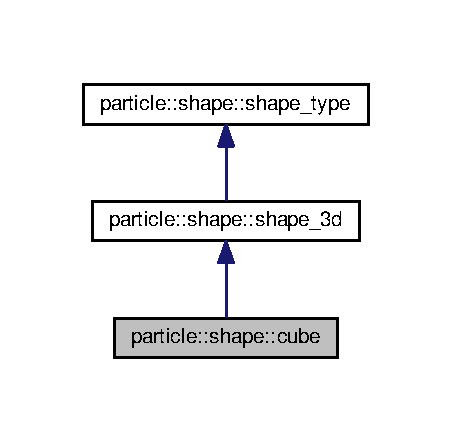
\includegraphics[width=217pt]{d6/dc4/classparticle_1_1shape_1_1cube__inherit__graph}
\end{center}
\end{figure}


Collaboration diagram for particle\+:\+:shape\+:\+:cube\+:\nopagebreak
\begin{figure}[H]
\begin{center}
\leavevmode
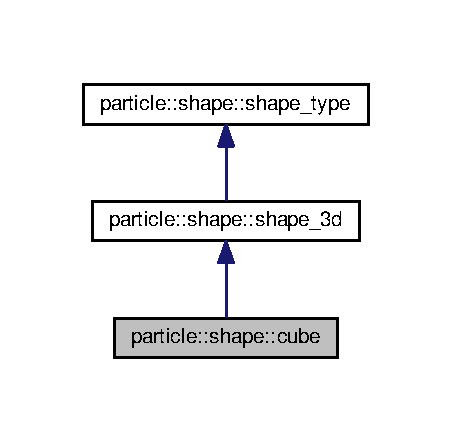
\includegraphics[width=217pt]{d9/d6b/classparticle_1_1shape_1_1cube__coll__graph}
\end{center}
\end{figure}
\subsection*{Public Member Functions}
\begin{DoxyCompactItemize}
\item 
\hyperlink{classparticle_1_1shape_1_1cube_a25e9690466125d4d09acdc79b354659c}{cube} ()
\begin{DoxyCompactList}\small\item\em Default constructor. \end{DoxyCompactList}\item 
\hyperlink{classparticle_1_1shape_1_1cube_a551fa11231e43fa349cd9b97e4f4a50e}{$\sim$cube} ()
\begin{DoxyCompactList}\small\item\em Default destructor. \end{DoxyCompactList}\end{DoxyCompactItemize}


\subsection{Detailed Description}
Cubic paritcle. 

\subsection{Constructor \& Destructor Documentation}
\index{particle\+::shape\+::cube@{particle\+::shape\+::cube}!cube@{cube}}
\index{cube@{cube}!particle\+::shape\+::cube@{particle\+::shape\+::cube}}
\subsubsection[{\texorpdfstring{cube()}{cube()}}]{\setlength{\rightskip}{0pt plus 5cm}particle\+::shape\+::cube\+::cube (
\begin{DoxyParamCaption}
{}
\end{DoxyParamCaption}
)\hspace{0.3cm}{\ttfamily [inline]}}\hypertarget{classparticle_1_1shape_1_1cube_a25e9690466125d4d09acdc79b354659c}{}\label{classparticle_1_1shape_1_1cube_a25e9690466125d4d09acdc79b354659c}


Default constructor. 

\index{particle\+::shape\+::cube@{particle\+::shape\+::cube}!````~cube@{$\sim$cube}}
\index{````~cube@{$\sim$cube}!particle\+::shape\+::cube@{particle\+::shape\+::cube}}
\subsubsection[{\texorpdfstring{$\sim$cube()}{~cube()}}]{\setlength{\rightskip}{0pt plus 5cm}particle\+::shape\+::cube\+::$\sim$cube (
\begin{DoxyParamCaption}
{}
\end{DoxyParamCaption}
)\hspace{0.3cm}{\ttfamily [inline]}}\hypertarget{classparticle_1_1shape_1_1cube_a551fa11231e43fa349cd9b97e4f4a50e}{}\label{classparticle_1_1shape_1_1cube_a551fa11231e43fa349cd9b97e4f4a50e}


Default destructor. 



The documentation for this class was generated from the following file\+:\begin{DoxyCompactItemize}
\item 
includes/\hyperlink{shape_8hpp}{shape.\+hpp}\end{DoxyCompactItemize}

\hypertarget{classfield__2d}{}\section{field\+\_\+2d Class Reference}
\label{classfield__2d}\index{field\+\_\+2d@{field\+\_\+2d}}


{\ttfamily \#include $<$field\+\_\+type.\+hpp$>$}



Inheritance diagram for field\+\_\+2d\+:
\nopagebreak
\begin{figure}[H]
\begin{center}
\leavevmode
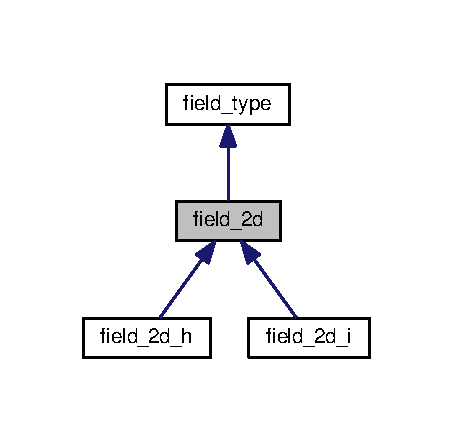
\includegraphics[width=218pt]{d1/de5/classfield__2d__inherit__graph}
\end{center}
\end{figure}


Collaboration diagram for field\+\_\+2d\+:
\nopagebreak
\begin{figure}[H]
\begin{center}
\leavevmode
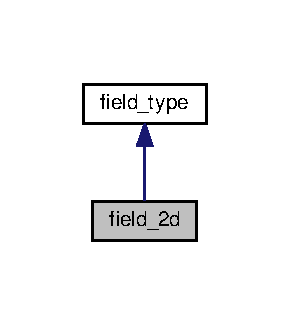
\includegraphics[width=139pt]{d4/d0c/classfield__2d__coll__graph}
\end{center}
\end{figure}
\subsection*{Public Member Functions}
\begin{DoxyCompactItemize}
\item 
\hyperlink{classfield__2d_ace254a4388aa5b73474b3929a47203de}{field\+\_\+2d} ()
\item 
\hyperlink{classfield__2d_a5ee3c13a181becb6103beb134300810d}{$\sim$field\+\_\+2d} ()
\item 
void \hyperlink{classfield__2d_adc2d76f3e57b4416010b50c8b33016d9}{next} (bool \&finish, std\+::vector$<$ int $>$ \&pos)
\item 
bool \hyperlink{classfield__2d_a72e41b87dc96e59d6bc636cc1a4ca44d}{check\+\_\+zero} (std\+::vector$<$ int $>$ \&position)
\item 
void \hyperlink{classfield__2d_abb312ba752786fb772ebcb4fba562224}{get\+\_\+2dzero} (bool $\ast$$\ast$\&x) const 
\item 
int \hyperlink{classfield__2d_a8fad4b75a1b1e3f2808a265152aab840}{findnum} ()
\end{DoxyCompactItemize}
\subsection*{Protected Attributes}
\begin{DoxyCompactItemize}
\item 
bool $\ast$$\ast$ \hyperlink{classfield__2d_ad1d58a5f2c6f3eb2d1ef656db977baa5}{iszero}
\end{DoxyCompactItemize}


\subsection{Constructor \& Destructor Documentation}
\index{field\+\_\+2d@{field\+\_\+2d}!field\+\_\+2d@{field\+\_\+2d}}
\index{field\+\_\+2d@{field\+\_\+2d}!field\+\_\+2d@{field\+\_\+2d}}
\subsubsection[{\texorpdfstring{field\+\_\+2d()}{field_2d()}}]{\setlength{\rightskip}{0pt plus 5cm}field\+\_\+2d\+::field\+\_\+2d (
\begin{DoxyParamCaption}
{}
\end{DoxyParamCaption}
)\hspace{0.3cm}{\ttfamily [inline]}}\hypertarget{classfield__2d_ace254a4388aa5b73474b3929a47203de}{}\label{classfield__2d_ace254a4388aa5b73474b3929a47203de}
\index{field\+\_\+2d@{field\+\_\+2d}!````~field\+\_\+2d@{$\sim$field\+\_\+2d}}
\index{````~field\+\_\+2d@{$\sim$field\+\_\+2d}!field\+\_\+2d@{field\+\_\+2d}}
\subsubsection[{\texorpdfstring{$\sim$field\+\_\+2d()}{~field_2d()}}]{\setlength{\rightskip}{0pt plus 5cm}field\+\_\+2d\+::$\sim$field\+\_\+2d (
\begin{DoxyParamCaption}
{}
\end{DoxyParamCaption}
)\hspace{0.3cm}{\ttfamily [inline]}}\hypertarget{classfield__2d_a5ee3c13a181becb6103beb134300810d}{}\label{classfield__2d_a5ee3c13a181becb6103beb134300810d}


\subsection{Member Function Documentation}
\index{field\+\_\+2d@{field\+\_\+2d}!check\+\_\+zero@{check\+\_\+zero}}
\index{check\+\_\+zero@{check\+\_\+zero}!field\+\_\+2d@{field\+\_\+2d}}
\subsubsection[{\texorpdfstring{check\+\_\+zero(std\+::vector$<$ int $>$ \&position)}{check_zero(std::vector< int > &position)}}]{\setlength{\rightskip}{0pt plus 5cm}bool field\+\_\+2d\+::check\+\_\+zero (
\begin{DoxyParamCaption}
\item[{std\+::vector$<$ int $>$ \&}]{position}
\end{DoxyParamCaption}
)\hspace{0.3cm}{\ttfamily [inline]}, {\ttfamily [virtual]}}\hypertarget{classfield__2d_a72e41b87dc96e59d6bc636cc1a4ca44d}{}\label{classfield__2d_a72e41b87dc96e59d6bc636cc1a4ca44d}


Reimplemented from \hyperlink{classfield__type_a8aabf0f54a8dc73b1ac529a26604c827}{field\+\_\+type}.

\index{field\+\_\+2d@{field\+\_\+2d}!findnum@{findnum}}
\index{findnum@{findnum}!field\+\_\+2d@{field\+\_\+2d}}
\subsubsection[{\texorpdfstring{findnum()}{findnum()}}]{\setlength{\rightskip}{0pt plus 5cm}int field\+\_\+2d\+::findnum (
\begin{DoxyParamCaption}
{}
\end{DoxyParamCaption}
)\hspace{0.3cm}{\ttfamily [virtual]}}\hypertarget{classfield__2d_a8fad4b75a1b1e3f2808a265152aab840}{}\label{classfield__2d_a8fad4b75a1b1e3f2808a265152aab840}


Reimplemented from \hyperlink{classfield__type_a73e5605cfd2714b2a358d61c4b102883}{field\+\_\+type}.

\index{field\+\_\+2d@{field\+\_\+2d}!get\+\_\+2dzero@{get\+\_\+2dzero}}
\index{get\+\_\+2dzero@{get\+\_\+2dzero}!field\+\_\+2d@{field\+\_\+2d}}
\subsubsection[{\texorpdfstring{get\+\_\+2dzero(bool $\ast$$\ast$\&x) const }{get_2dzero(bool **&x) const }}]{\setlength{\rightskip}{0pt plus 5cm}void field\+\_\+2d\+::get\+\_\+2dzero (
\begin{DoxyParamCaption}
\item[{bool $\ast$$\ast$\&}]{x}
\end{DoxyParamCaption}
) const\hspace{0.3cm}{\ttfamily [inline]}, {\ttfamily [virtual]}}\hypertarget{classfield__2d_abb312ba752786fb772ebcb4fba562224}{}\label{classfield__2d_abb312ba752786fb772ebcb4fba562224}


Reimplemented from \hyperlink{classfield__type_a4924396b413bb7f5a43e6602561bdfbf}{field\+\_\+type}.

\index{field\+\_\+2d@{field\+\_\+2d}!next@{next}}
\index{next@{next}!field\+\_\+2d@{field\+\_\+2d}}
\subsubsection[{\texorpdfstring{next(bool \&finish, std\+::vector$<$ int $>$ \&pos)}{next(bool &finish, std::vector< int > &pos)}}]{\setlength{\rightskip}{0pt plus 5cm}void field\+\_\+2d\+::next (
\begin{DoxyParamCaption}
\item[{bool \&}]{finish, }
\item[{std\+::vector$<$ int $>$ \&}]{pos}
\end{DoxyParamCaption}
)\hspace{0.3cm}{\ttfamily [virtual]}}\hypertarget{classfield__2d_adc2d76f3e57b4416010b50c8b33016d9}{}\label{classfield__2d_adc2d76f3e57b4416010b50c8b33016d9}


Reimplemented from \hyperlink{classfield__type_afaf4b3449a0ee906ebe543439054eab5}{field\+\_\+type}.



\subsection{Member Data Documentation}
\index{field\+\_\+2d@{field\+\_\+2d}!iszero@{iszero}}
\index{iszero@{iszero}!field\+\_\+2d@{field\+\_\+2d}}
\subsubsection[{\texorpdfstring{iszero}{iszero}}]{\setlength{\rightskip}{0pt plus 5cm}bool$\ast$$\ast$ field\+\_\+2d\+::iszero\hspace{0.3cm}{\ttfamily [protected]}}\hypertarget{classfield__2d_ad1d58a5f2c6f3eb2d1ef656db977baa5}{}\label{classfield__2d_ad1d58a5f2c6f3eb2d1ef656db977baa5}


The documentation for this class was generated from the following file\+:\begin{DoxyCompactItemize}
\item 
includes/\hyperlink{field__type_8hpp}{field\+\_\+type.\+hpp}\end{DoxyCompactItemize}

\hypertarget{classfield__2d__h}{}\section{field\+\_\+2d\+\_\+h Class Reference}
\label{classfield__2d__h}\index{field\+\_\+2d\+\_\+h@{field\+\_\+2d\+\_\+h}}


{\ttfamily \#include $<$field\+\_\+type.\+hpp$>$}



Inheritance diagram for field\+\_\+2d\+\_\+h\+:
\nopagebreak
\begin{figure}[H]
\begin{center}
\leavevmode
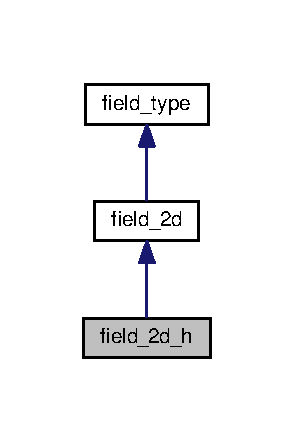
\includegraphics[width=141pt]{df/dde/classfield__2d__h__inherit__graph}
\end{center}
\end{figure}


Collaboration diagram for field\+\_\+2d\+\_\+h\+:
\nopagebreak
\begin{figure}[H]
\begin{center}
\leavevmode
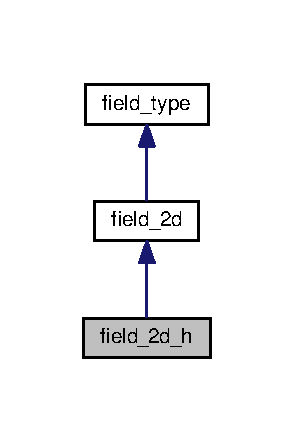
\includegraphics[width=141pt]{d2/d67/classfield__2d__h__coll__graph}
\end{center}
\end{figure}
\subsection*{Public Member Functions}
\begin{DoxyCompactItemize}
\item 
\hyperlink{classfield__2d__h_ab6df2859fe41bbb6f756e36bc3af9df1}{field\+\_\+2d\+\_\+h} ()
\item 
\hyperlink{classfield__2d__h_af181b94fc627c791b50d62e859aec52e}{field\+\_\+2d\+\_\+h} (int size, bool isperio)
\item 
\hyperlink{classfield__2d__h_a9a3c09f4ccb61e0d5e425588ed5604db}{field\+\_\+2d\+\_\+h} (int size, bool isperio, int p\+\_\+pad)
\item 
\hyperlink{classfield__2d__h_a4473565aacf919cb23929f85c776a9f3}{field\+\_\+2d\+\_\+h} (\hyperlink{classfield__type}{field\+\_\+type} \&other)
\item 
\hyperlink{classfield__2d__h_ae819170893baf55b926e81babbfd44bb}{field\+\_\+2d\+\_\+h} (const \hyperlink{classfield__2d__h}{field\+\_\+2d\+\_\+h} \&other)
\item 
\hyperlink{classfield__2d__h_ab3590bf885419149040f15c42fd9065d}{$\sim$field\+\_\+2d\+\_\+h} ()
\item 
void \hyperlink{classfield__2d__h_a48d8cd8baa2fb122428a949b6fef0be4}{h\+\_\+access} (std\+::vector$<$ int $>$ \&position, std\+::vector$<$ double $>$ \&out)
\item 
void \hyperlink{classfield__2d__h_aaad4e607d26bff240f87dc81b5b8139c}{h\+\_\+next} (bool \&finish, std\+::vector$<$ int $>$ \&pos, std\+::vector$<$ double $>$ \&out)
\item 
void \hyperlink{classfield__2d__h_a94fe388174d778328629ad3fb4c13566}{fill\+\_\+ghost} (int num\+\_\+rows)
\item 
\hyperlink{classfield__2d__h}{field\+\_\+2d\+\_\+h} \& \hyperlink{classfield__2d__h_acc8c8dc7a57734eb984d29a55608adf6}{operator=} (const \hyperlink{classfield__2d__h}{field\+\_\+2d\+\_\+h} \&other)
\item 
void \hyperlink{classfield__2d__h_a595cdddce98f5d61467606f824b4939e}{get\+\_\+2dfield\+\_\+h} (double $\ast$$\ast$\&x, double $\ast$$\ast$\&y, double $\ast$$\ast$\&z) const 
\item 
void \hyperlink{classfield__2d__h_a450df16021eea9c91f7ddab116f69ef7}{h\+\_\+adjacent} (std\+::vector$<$ int $>$ \&position, double $\ast$$\ast$out)
\item 
void \hyperlink{classfield__2d__h_a3a4c57fdf1ce84f4e6006bb37a76ec58}{fill\+\_\+rand} (std\+::vector$<$ int $>$ \&position)
\item 
void \hyperlink{classfield__2d__h_ac4ef3e08335182c46bfb6ff37cf447cd}{fill\+\_\+one} (std\+::vector$<$ int $>$ \&position)
\item 
void \hyperlink{classfield__2d__h_aa95c0be540a84b7a2365720ffc0c4520}{fill\+\_\+zero} (std\+::vector$<$ int $>$ \&position)
\item 
void \hyperlink{classfield__2d__h_a9a0a35285e1a3995e2768a8b43c4855a}{fill\+\_\+val\+\_\+h} (std\+::vector$<$ int $>$ \&position, double x, double y, double z)
\item 
void \hyperlink{classfield__2d__h_aa8777664592ab4317bca3734497e2404}{add\+\_\+val\+\_\+h} (std\+::vector$<$ int $>$ \&position, std\+::vector$<$ double $>$ \&in)
\item 
void \hyperlink{classfield__2d__h_a87173eff35d950aeb70b0c955c5c0e5d}{change\+\_\+to\+\_\+test} (std\+::vector$<$ int $>$ \&position, \hyperlink{classham__type}{ham\+\_\+type} $\ast$hamil)
\item 
void \hyperlink{classfield__2d__h_a9705fcf4d6fafbac4d2b37778a97fd00}{send\+\_\+data} (int dest\+\_\+rank)
\item 
void \hyperlink{classfield__2d__h_a04ab343341666fa7f237f953f963cda3}{recv\+\_\+data} (int src\+\_\+rank)
\end{DoxyCompactItemize}
\subsection*{Protected Attributes}
\begin{DoxyCompactItemize}
\item 
double $\ast$$\ast$ \hyperlink{classfield__2d__h_aa2763f7d369420b8baca0d34c885deab}{spinx}
\item 
double $\ast$$\ast$ \hyperlink{classfield__2d__h_a13c1fcf346bb1fac2ae507b494864bfb}{spiny}
\item 
double $\ast$$\ast$ \hyperlink{classfield__2d__h_a370ec3121a04ddf7e17f95540bbe5517}{spinz}
\item 
int \hyperlink{classfield__2d__h_ab20f326cbd41670086b78939dc21f370}{dirsx} \mbox{[}4\mbox{]}
\item 
int \hyperlink{classfield__2d__h_a8a316de6115eaba1dbde1f8f6a47fd2b}{dirsy} \mbox{[}4\mbox{]}
\end{DoxyCompactItemize}


\subsection{Constructor \& Destructor Documentation}
\index{field\+\_\+2d\+\_\+h@{field\+\_\+2d\+\_\+h}!field\+\_\+2d\+\_\+h@{field\+\_\+2d\+\_\+h}}
\index{field\+\_\+2d\+\_\+h@{field\+\_\+2d\+\_\+h}!field\+\_\+2d\+\_\+h@{field\+\_\+2d\+\_\+h}}
\subsubsection[{\texorpdfstring{field\+\_\+2d\+\_\+h()}{field_2d_h()}}]{\setlength{\rightskip}{0pt plus 5cm}field\+\_\+2d\+\_\+h\+::field\+\_\+2d\+\_\+h (
\begin{DoxyParamCaption}
{}
\end{DoxyParamCaption}
)}\hypertarget{classfield__2d__h_ab6df2859fe41bbb6f756e36bc3af9df1}{}\label{classfield__2d__h_ab6df2859fe41bbb6f756e36bc3af9df1}
\index{field\+\_\+2d\+\_\+h@{field\+\_\+2d\+\_\+h}!field\+\_\+2d\+\_\+h@{field\+\_\+2d\+\_\+h}}
\index{field\+\_\+2d\+\_\+h@{field\+\_\+2d\+\_\+h}!field\+\_\+2d\+\_\+h@{field\+\_\+2d\+\_\+h}}
\subsubsection[{\texorpdfstring{field\+\_\+2d\+\_\+h(int size, bool isperio)}{field_2d_h(int size, bool isperio)}}]{\setlength{\rightskip}{0pt plus 5cm}field\+\_\+2d\+\_\+h\+::field\+\_\+2d\+\_\+h (
\begin{DoxyParamCaption}
\item[{int}]{size, }
\item[{bool}]{isperio}
\end{DoxyParamCaption}
)}\hypertarget{classfield__2d__h_af181b94fc627c791b50d62e859aec52e}{}\label{classfield__2d__h_af181b94fc627c791b50d62e859aec52e}
\index{field\+\_\+2d\+\_\+h@{field\+\_\+2d\+\_\+h}!field\+\_\+2d\+\_\+h@{field\+\_\+2d\+\_\+h}}
\index{field\+\_\+2d\+\_\+h@{field\+\_\+2d\+\_\+h}!field\+\_\+2d\+\_\+h@{field\+\_\+2d\+\_\+h}}
\subsubsection[{\texorpdfstring{field\+\_\+2d\+\_\+h(int size, bool isperio, int p\+\_\+pad)}{field_2d_h(int size, bool isperio, int p_pad)}}]{\setlength{\rightskip}{0pt plus 5cm}field\+\_\+2d\+\_\+h\+::field\+\_\+2d\+\_\+h (
\begin{DoxyParamCaption}
\item[{int}]{size, }
\item[{bool}]{isperio, }
\item[{int}]{p\+\_\+pad}
\end{DoxyParamCaption}
)}\hypertarget{classfield__2d__h_a9a3c09f4ccb61e0d5e425588ed5604db}{}\label{classfield__2d__h_a9a3c09f4ccb61e0d5e425588ed5604db}
\index{field\+\_\+2d\+\_\+h@{field\+\_\+2d\+\_\+h}!field\+\_\+2d\+\_\+h@{field\+\_\+2d\+\_\+h}}
\index{field\+\_\+2d\+\_\+h@{field\+\_\+2d\+\_\+h}!field\+\_\+2d\+\_\+h@{field\+\_\+2d\+\_\+h}}
\subsubsection[{\texorpdfstring{field\+\_\+2d\+\_\+h(field\+\_\+type \&other)}{field_2d_h(field_type &other)}}]{\setlength{\rightskip}{0pt plus 5cm}field\+\_\+2d\+\_\+h\+::field\+\_\+2d\+\_\+h (
\begin{DoxyParamCaption}
\item[{{\bf field\+\_\+type} \&}]{other}
\end{DoxyParamCaption}
)}\hypertarget{classfield__2d__h_a4473565aacf919cb23929f85c776a9f3}{}\label{classfield__2d__h_a4473565aacf919cb23929f85c776a9f3}
\index{field\+\_\+2d\+\_\+h@{field\+\_\+2d\+\_\+h}!field\+\_\+2d\+\_\+h@{field\+\_\+2d\+\_\+h}}
\index{field\+\_\+2d\+\_\+h@{field\+\_\+2d\+\_\+h}!field\+\_\+2d\+\_\+h@{field\+\_\+2d\+\_\+h}}
\subsubsection[{\texorpdfstring{field\+\_\+2d\+\_\+h(const field\+\_\+2d\+\_\+h \&other)}{field_2d_h(const field_2d_h &other)}}]{\setlength{\rightskip}{0pt plus 5cm}field\+\_\+2d\+\_\+h\+::field\+\_\+2d\+\_\+h (
\begin{DoxyParamCaption}
\item[{const {\bf field\+\_\+2d\+\_\+h} \&}]{other}
\end{DoxyParamCaption}
)}\hypertarget{classfield__2d__h_ae819170893baf55b926e81babbfd44bb}{}\label{classfield__2d__h_ae819170893baf55b926e81babbfd44bb}
\index{field\+\_\+2d\+\_\+h@{field\+\_\+2d\+\_\+h}!````~field\+\_\+2d\+\_\+h@{$\sim$field\+\_\+2d\+\_\+h}}
\index{````~field\+\_\+2d\+\_\+h@{$\sim$field\+\_\+2d\+\_\+h}!field\+\_\+2d\+\_\+h@{field\+\_\+2d\+\_\+h}}
\subsubsection[{\texorpdfstring{$\sim$field\+\_\+2d\+\_\+h()}{~field_2d_h()}}]{\setlength{\rightskip}{0pt plus 5cm}field\+\_\+2d\+\_\+h\+::$\sim$field\+\_\+2d\+\_\+h (
\begin{DoxyParamCaption}
{}
\end{DoxyParamCaption}
)}\hypertarget{classfield__2d__h_ab3590bf885419149040f15c42fd9065d}{}\label{classfield__2d__h_ab3590bf885419149040f15c42fd9065d}


\subsection{Member Function Documentation}
\index{field\+\_\+2d\+\_\+h@{field\+\_\+2d\+\_\+h}!add\+\_\+val\+\_\+h@{add\+\_\+val\+\_\+h}}
\index{add\+\_\+val\+\_\+h@{add\+\_\+val\+\_\+h}!field\+\_\+2d\+\_\+h@{field\+\_\+2d\+\_\+h}}
\subsubsection[{\texorpdfstring{add\+\_\+val\+\_\+h(std\+::vector$<$ int $>$ \&position, std\+::vector$<$ double $>$ \&in)}{add_val_h(std::vector< int > &position, std::vector< double > &in)}}]{\setlength{\rightskip}{0pt plus 5cm}void field\+\_\+2d\+\_\+h\+::add\+\_\+val\+\_\+h (
\begin{DoxyParamCaption}
\item[{std\+::vector$<$ int $>$ \&}]{position, }
\item[{std\+::vector$<$ double $>$ \&}]{in}
\end{DoxyParamCaption}
)\hspace{0.3cm}{\ttfamily [virtual]}}\hypertarget{classfield__2d__h_aa8777664592ab4317bca3734497e2404}{}\label{classfield__2d__h_aa8777664592ab4317bca3734497e2404}


Reimplemented from \hyperlink{classfield__type_a35a20297e1cddac40d4c2aecef5a5594}{field\+\_\+type}.

\index{field\+\_\+2d\+\_\+h@{field\+\_\+2d\+\_\+h}!change\+\_\+to\+\_\+test@{change\+\_\+to\+\_\+test}}
\index{change\+\_\+to\+\_\+test@{change\+\_\+to\+\_\+test}!field\+\_\+2d\+\_\+h@{field\+\_\+2d\+\_\+h}}
\subsubsection[{\texorpdfstring{change\+\_\+to\+\_\+test(std\+::vector$<$ int $>$ \&position, ham\+\_\+type $\ast$hamil)}{change_to_test(std::vector< int > &position, ham_type *hamil)}}]{\setlength{\rightskip}{0pt plus 5cm}void field\+\_\+2d\+\_\+h\+::change\+\_\+to\+\_\+test (
\begin{DoxyParamCaption}
\item[{std\+::vector$<$ int $>$ \&}]{position, }
\item[{{\bf ham\+\_\+type} $\ast$}]{hamil}
\end{DoxyParamCaption}
)\hspace{0.3cm}{\ttfamily [virtual]}}\hypertarget{classfield__2d__h_a87173eff35d950aeb70b0c955c5c0e5d}{}\label{classfield__2d__h_a87173eff35d950aeb70b0c955c5c0e5d}


Reimplemented from \hyperlink{classfield__type_a32140b8a785c0139dd27304143ca5f17}{field\+\_\+type}.

\index{field\+\_\+2d\+\_\+h@{field\+\_\+2d\+\_\+h}!fill\+\_\+ghost@{fill\+\_\+ghost}}
\index{fill\+\_\+ghost@{fill\+\_\+ghost}!field\+\_\+2d\+\_\+h@{field\+\_\+2d\+\_\+h}}
\subsubsection[{\texorpdfstring{fill\+\_\+ghost(int num\+\_\+rows)}{fill_ghost(int num_rows)}}]{\setlength{\rightskip}{0pt plus 5cm}void field\+\_\+2d\+\_\+h\+::fill\+\_\+ghost (
\begin{DoxyParamCaption}
\item[{int}]{num\+\_\+rows}
\end{DoxyParamCaption}
)\hspace{0.3cm}{\ttfamily [virtual]}}\hypertarget{classfield__2d__h_a94fe388174d778328629ad3fb4c13566}{}\label{classfield__2d__h_a94fe388174d778328629ad3fb4c13566}


Reimplemented from \hyperlink{classfield__type_a11c23271c828983406e8e80c66b81c46}{field\+\_\+type}.

\index{field\+\_\+2d\+\_\+h@{field\+\_\+2d\+\_\+h}!fill\+\_\+one@{fill\+\_\+one}}
\index{fill\+\_\+one@{fill\+\_\+one}!field\+\_\+2d\+\_\+h@{field\+\_\+2d\+\_\+h}}
\subsubsection[{\texorpdfstring{fill\+\_\+one(std\+::vector$<$ int $>$ \&position)}{fill_one(std::vector< int > &position)}}]{\setlength{\rightskip}{0pt plus 5cm}void field\+\_\+2d\+\_\+h\+::fill\+\_\+one (
\begin{DoxyParamCaption}
\item[{std\+::vector$<$ int $>$ \&}]{position}
\end{DoxyParamCaption}
)\hspace{0.3cm}{\ttfamily [virtual]}}\hypertarget{classfield__2d__h_ac4ef3e08335182c46bfb6ff37cf447cd}{}\label{classfield__2d__h_ac4ef3e08335182c46bfb6ff37cf447cd}


Reimplemented from \hyperlink{classfield__type_acb4fb5c3393feed8685eb3957c032a15}{field\+\_\+type}.

\index{field\+\_\+2d\+\_\+h@{field\+\_\+2d\+\_\+h}!fill\+\_\+rand@{fill\+\_\+rand}}
\index{fill\+\_\+rand@{fill\+\_\+rand}!field\+\_\+2d\+\_\+h@{field\+\_\+2d\+\_\+h}}
\subsubsection[{\texorpdfstring{fill\+\_\+rand(std\+::vector$<$ int $>$ \&position)}{fill_rand(std::vector< int > &position)}}]{\setlength{\rightskip}{0pt plus 5cm}void field\+\_\+2d\+\_\+h\+::fill\+\_\+rand (
\begin{DoxyParamCaption}
\item[{std\+::vector$<$ int $>$ \&}]{position}
\end{DoxyParamCaption}
)\hspace{0.3cm}{\ttfamily [virtual]}}\hypertarget{classfield__2d__h_a3a4c57fdf1ce84f4e6006bb37a76ec58}{}\label{classfield__2d__h_a3a4c57fdf1ce84f4e6006bb37a76ec58}


Reimplemented from \hyperlink{classfield__type_a87d6bf8e9e97ce158a356fefaddc3bee}{field\+\_\+type}.

\index{field\+\_\+2d\+\_\+h@{field\+\_\+2d\+\_\+h}!fill\+\_\+val\+\_\+h@{fill\+\_\+val\+\_\+h}}
\index{fill\+\_\+val\+\_\+h@{fill\+\_\+val\+\_\+h}!field\+\_\+2d\+\_\+h@{field\+\_\+2d\+\_\+h}}
\subsubsection[{\texorpdfstring{fill\+\_\+val\+\_\+h(std\+::vector$<$ int $>$ \&position, double x, double y, double z)}{fill_val_h(std::vector< int > &position, double x, double y, double z)}}]{\setlength{\rightskip}{0pt plus 5cm}void field\+\_\+2d\+\_\+h\+::fill\+\_\+val\+\_\+h (
\begin{DoxyParamCaption}
\item[{std\+::vector$<$ int $>$ \&}]{position, }
\item[{double}]{x, }
\item[{double}]{y, }
\item[{double}]{z}
\end{DoxyParamCaption}
)\hspace{0.3cm}{\ttfamily [virtual]}}\hypertarget{classfield__2d__h_a9a0a35285e1a3995e2768a8b43c4855a}{}\label{classfield__2d__h_a9a0a35285e1a3995e2768a8b43c4855a}


Reimplemented from \hyperlink{classfield__type_a02500bfb9021cf13ff6e1be66b63b9ae}{field\+\_\+type}.

\index{field\+\_\+2d\+\_\+h@{field\+\_\+2d\+\_\+h}!fill\+\_\+zero@{fill\+\_\+zero}}
\index{fill\+\_\+zero@{fill\+\_\+zero}!field\+\_\+2d\+\_\+h@{field\+\_\+2d\+\_\+h}}
\subsubsection[{\texorpdfstring{fill\+\_\+zero(std\+::vector$<$ int $>$ \&position)}{fill_zero(std::vector< int > &position)}}]{\setlength{\rightskip}{0pt plus 5cm}void field\+\_\+2d\+\_\+h\+::fill\+\_\+zero (
\begin{DoxyParamCaption}
\item[{std\+::vector$<$ int $>$ \&}]{position}
\end{DoxyParamCaption}
)\hspace{0.3cm}{\ttfamily [virtual]}}\hypertarget{classfield__2d__h_aa95c0be540a84b7a2365720ffc0c4520}{}\label{classfield__2d__h_aa95c0be540a84b7a2365720ffc0c4520}


Reimplemented from \hyperlink{classfield__type_afdb5b29e839fa11c7faeff60ee49aebb}{field\+\_\+type}.

\index{field\+\_\+2d\+\_\+h@{field\+\_\+2d\+\_\+h}!get\+\_\+2dfield\+\_\+h@{get\+\_\+2dfield\+\_\+h}}
\index{get\+\_\+2dfield\+\_\+h@{get\+\_\+2dfield\+\_\+h}!field\+\_\+2d\+\_\+h@{field\+\_\+2d\+\_\+h}}
\subsubsection[{\texorpdfstring{get\+\_\+2dfield\+\_\+h(double $\ast$$\ast$\&x, double $\ast$$\ast$\&y, double $\ast$$\ast$\&z) const }{get_2dfield_h(double **&x, double **&y, double **&z) const }}]{\setlength{\rightskip}{0pt plus 5cm}void field\+\_\+2d\+\_\+h\+::get\+\_\+2dfield\+\_\+h (
\begin{DoxyParamCaption}
\item[{double $\ast$$\ast$\&}]{x, }
\item[{double $\ast$$\ast$\&}]{y, }
\item[{double $\ast$$\ast$\&}]{z}
\end{DoxyParamCaption}
) const\hspace{0.3cm}{\ttfamily [virtual]}}\hypertarget{classfield__2d__h_a595cdddce98f5d61467606f824b4939e}{}\label{classfield__2d__h_a595cdddce98f5d61467606f824b4939e}


Reimplemented from \hyperlink{classfield__type_af15dfa4de69c756148f82628b095b22e}{field\+\_\+type}.

\index{field\+\_\+2d\+\_\+h@{field\+\_\+2d\+\_\+h}!h\+\_\+access@{h\+\_\+access}}
\index{h\+\_\+access@{h\+\_\+access}!field\+\_\+2d\+\_\+h@{field\+\_\+2d\+\_\+h}}
\subsubsection[{\texorpdfstring{h\+\_\+access(std\+::vector$<$ int $>$ \&position, std\+::vector$<$ double $>$ \&out)}{h_access(std::vector< int > &position, std::vector< double > &out)}}]{\setlength{\rightskip}{0pt plus 5cm}void field\+\_\+2d\+\_\+h\+::h\+\_\+access (
\begin{DoxyParamCaption}
\item[{std\+::vector$<$ int $>$ \&}]{position, }
\item[{std\+::vector$<$ double $>$ \&}]{out}
\end{DoxyParamCaption}
)\hspace{0.3cm}{\ttfamily [virtual]}}\hypertarget{classfield__2d__h_a48d8cd8baa2fb122428a949b6fef0be4}{}\label{classfield__2d__h_a48d8cd8baa2fb122428a949b6fef0be4}


Reimplemented from \hyperlink{classfield__type_ada65523f1a000cbd929f2d97d747fa59}{field\+\_\+type}.

\index{field\+\_\+2d\+\_\+h@{field\+\_\+2d\+\_\+h}!h\+\_\+adjacent@{h\+\_\+adjacent}}
\index{h\+\_\+adjacent@{h\+\_\+adjacent}!field\+\_\+2d\+\_\+h@{field\+\_\+2d\+\_\+h}}
\subsubsection[{\texorpdfstring{h\+\_\+adjacent(std\+::vector$<$ int $>$ \&position, double $\ast$$\ast$out)}{h_adjacent(std::vector< int > &position, double **out)}}]{\setlength{\rightskip}{0pt plus 5cm}void field\+\_\+2d\+\_\+h\+::h\+\_\+adjacent (
\begin{DoxyParamCaption}
\item[{std\+::vector$<$ int $>$ \&}]{position, }
\item[{double $\ast$$\ast$}]{out}
\end{DoxyParamCaption}
)\hspace{0.3cm}{\ttfamily [virtual]}}\hypertarget{classfield__2d__h_a450df16021eea9c91f7ddab116f69ef7}{}\label{classfield__2d__h_a450df16021eea9c91f7ddab116f69ef7}


Reimplemented from \hyperlink{classfield__type_af91a0a4b7d3076c41baa96f25faec0c4}{field\+\_\+type}.

\index{field\+\_\+2d\+\_\+h@{field\+\_\+2d\+\_\+h}!h\+\_\+next@{h\+\_\+next}}
\index{h\+\_\+next@{h\+\_\+next}!field\+\_\+2d\+\_\+h@{field\+\_\+2d\+\_\+h}}
\subsubsection[{\texorpdfstring{h\+\_\+next(bool \&finish, std\+::vector$<$ int $>$ \&pos, std\+::vector$<$ double $>$ \&out)}{h_next(bool &finish, std::vector< int > &pos, std::vector< double > &out)}}]{\setlength{\rightskip}{0pt plus 5cm}void field\+\_\+2d\+\_\+h\+::h\+\_\+next (
\begin{DoxyParamCaption}
\item[{bool \&}]{finish, }
\item[{std\+::vector$<$ int $>$ \&}]{pos, }
\item[{std\+::vector$<$ double $>$ \&}]{out}
\end{DoxyParamCaption}
)\hspace{0.3cm}{\ttfamily [virtual]}}\hypertarget{classfield__2d__h_aaad4e607d26bff240f87dc81b5b8139c}{}\label{classfield__2d__h_aaad4e607d26bff240f87dc81b5b8139c}


Reimplemented from \hyperlink{classfield__type_a4f68c166bbd86806584f44c6d6faf50f}{field\+\_\+type}.

\index{field\+\_\+2d\+\_\+h@{field\+\_\+2d\+\_\+h}!operator=@{operator=}}
\index{operator=@{operator=}!field\+\_\+2d\+\_\+h@{field\+\_\+2d\+\_\+h}}
\subsubsection[{\texorpdfstring{operator=(const field\+\_\+2d\+\_\+h \&other)}{operator=(const field_2d_h &other)}}]{\setlength{\rightskip}{0pt plus 5cm}{\bf field\+\_\+2d\+\_\+h}\& field\+\_\+2d\+\_\+h\+::operator= (
\begin{DoxyParamCaption}
\item[{const {\bf field\+\_\+2d\+\_\+h} \&}]{other}
\end{DoxyParamCaption}
)}\hypertarget{classfield__2d__h_acc8c8dc7a57734eb984d29a55608adf6}{}\label{classfield__2d__h_acc8c8dc7a57734eb984d29a55608adf6}
\index{field\+\_\+2d\+\_\+h@{field\+\_\+2d\+\_\+h}!recv\+\_\+data@{recv\+\_\+data}}
\index{recv\+\_\+data@{recv\+\_\+data}!field\+\_\+2d\+\_\+h@{field\+\_\+2d\+\_\+h}}
\subsubsection[{\texorpdfstring{recv\+\_\+data(int src\+\_\+rank)}{recv_data(int src_rank)}}]{\setlength{\rightskip}{0pt plus 5cm}void field\+\_\+2d\+\_\+h\+::recv\+\_\+data (
\begin{DoxyParamCaption}
\item[{int}]{src\+\_\+rank}
\end{DoxyParamCaption}
)\hspace{0.3cm}{\ttfamily [virtual]}}\hypertarget{classfield__2d__h_a04ab343341666fa7f237f953f963cda3}{}\label{classfield__2d__h_a04ab343341666fa7f237f953f963cda3}


Reimplemented from \hyperlink{classfield__type_ac29bf02760384b80a08e5e57ca43542f}{field\+\_\+type}.

\index{field\+\_\+2d\+\_\+h@{field\+\_\+2d\+\_\+h}!send\+\_\+data@{send\+\_\+data}}
\index{send\+\_\+data@{send\+\_\+data}!field\+\_\+2d\+\_\+h@{field\+\_\+2d\+\_\+h}}
\subsubsection[{\texorpdfstring{send\+\_\+data(int dest\+\_\+rank)}{send_data(int dest_rank)}}]{\setlength{\rightskip}{0pt plus 5cm}void field\+\_\+2d\+\_\+h\+::send\+\_\+data (
\begin{DoxyParamCaption}
\item[{int}]{dest\+\_\+rank}
\end{DoxyParamCaption}
)\hspace{0.3cm}{\ttfamily [virtual]}}\hypertarget{classfield__2d__h_a9705fcf4d6fafbac4d2b37778a97fd00}{}\label{classfield__2d__h_a9705fcf4d6fafbac4d2b37778a97fd00}


Reimplemented from \hyperlink{classfield__type_afaabc410e2ce254c23e3c4aa39d1916d}{field\+\_\+type}.



\subsection{Member Data Documentation}
\index{field\+\_\+2d\+\_\+h@{field\+\_\+2d\+\_\+h}!dirsx@{dirsx}}
\index{dirsx@{dirsx}!field\+\_\+2d\+\_\+h@{field\+\_\+2d\+\_\+h}}
\subsubsection[{\texorpdfstring{dirsx}{dirsx}}]{\setlength{\rightskip}{0pt plus 5cm}int field\+\_\+2d\+\_\+h\+::dirsx\mbox{[}4\mbox{]}\hspace{0.3cm}{\ttfamily [protected]}}\hypertarget{classfield__2d__h_ab20f326cbd41670086b78939dc21f370}{}\label{classfield__2d__h_ab20f326cbd41670086b78939dc21f370}
\index{field\+\_\+2d\+\_\+h@{field\+\_\+2d\+\_\+h}!dirsy@{dirsy}}
\index{dirsy@{dirsy}!field\+\_\+2d\+\_\+h@{field\+\_\+2d\+\_\+h}}
\subsubsection[{\texorpdfstring{dirsy}{dirsy}}]{\setlength{\rightskip}{0pt plus 5cm}int field\+\_\+2d\+\_\+h\+::dirsy\mbox{[}4\mbox{]}\hspace{0.3cm}{\ttfamily [protected]}}\hypertarget{classfield__2d__h_a8a316de6115eaba1dbde1f8f6a47fd2b}{}\label{classfield__2d__h_a8a316de6115eaba1dbde1f8f6a47fd2b}
\index{field\+\_\+2d\+\_\+h@{field\+\_\+2d\+\_\+h}!spinx@{spinx}}
\index{spinx@{spinx}!field\+\_\+2d\+\_\+h@{field\+\_\+2d\+\_\+h}}
\subsubsection[{\texorpdfstring{spinx}{spinx}}]{\setlength{\rightskip}{0pt plus 5cm}double$\ast$$\ast$ field\+\_\+2d\+\_\+h\+::spinx\hspace{0.3cm}{\ttfamily [protected]}}\hypertarget{classfield__2d__h_aa2763f7d369420b8baca0d34c885deab}{}\label{classfield__2d__h_aa2763f7d369420b8baca0d34c885deab}
\index{field\+\_\+2d\+\_\+h@{field\+\_\+2d\+\_\+h}!spiny@{spiny}}
\index{spiny@{spiny}!field\+\_\+2d\+\_\+h@{field\+\_\+2d\+\_\+h}}
\subsubsection[{\texorpdfstring{spiny}{spiny}}]{\setlength{\rightskip}{0pt plus 5cm}double$\ast$$\ast$ field\+\_\+2d\+\_\+h\+::spiny\hspace{0.3cm}{\ttfamily [protected]}}\hypertarget{classfield__2d__h_a13c1fcf346bb1fac2ae507b494864bfb}{}\label{classfield__2d__h_a13c1fcf346bb1fac2ae507b494864bfb}
\index{field\+\_\+2d\+\_\+h@{field\+\_\+2d\+\_\+h}!spinz@{spinz}}
\index{spinz@{spinz}!field\+\_\+2d\+\_\+h@{field\+\_\+2d\+\_\+h}}
\subsubsection[{\texorpdfstring{spinz}{spinz}}]{\setlength{\rightskip}{0pt plus 5cm}double$\ast$$\ast$ field\+\_\+2d\+\_\+h\+::spinz\hspace{0.3cm}{\ttfamily [protected]}}\hypertarget{classfield__2d__h_a370ec3121a04ddf7e17f95540bbe5517}{}\label{classfield__2d__h_a370ec3121a04ddf7e17f95540bbe5517}


The documentation for this class was generated from the following file\+:\begin{DoxyCompactItemize}
\item 
includes/\hyperlink{field__type_8hpp}{field\+\_\+type.\+hpp}\end{DoxyCompactItemize}

\hypertarget{classfield__2d__i}{}\section{field\+\_\+2d\+\_\+i Class Reference}
\label{classfield__2d__i}\index{field\+\_\+2d\+\_\+i@{field\+\_\+2d\+\_\+i}}


{\ttfamily \#include $<$field\+\_\+type.\+hpp$>$}



Inheritance diagram for field\+\_\+2d\+\_\+i\+:
\nopagebreak
\begin{figure}[H]
\begin{center}
\leavevmode
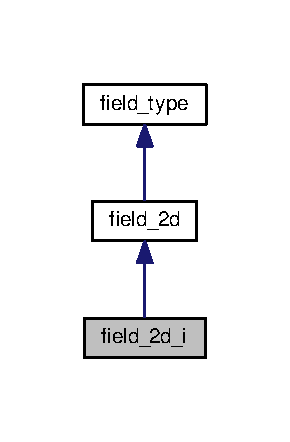
\includegraphics[width=139pt]{dd/d3f/classfield__2d__i__inherit__graph}
\end{center}
\end{figure}


Collaboration diagram for field\+\_\+2d\+\_\+i\+:
\nopagebreak
\begin{figure}[H]
\begin{center}
\leavevmode
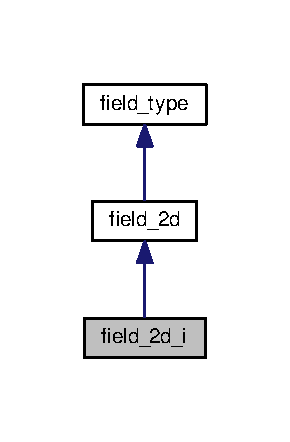
\includegraphics[width=139pt]{d4/d8c/classfield__2d__i__coll__graph}
\end{center}
\end{figure}
\subsection*{Public Member Functions}
\begin{DoxyCompactItemize}
\item 
\hyperlink{classfield__2d__i_ab7586ee4301dfa3b724cd6c6ffdc78e1}{field\+\_\+2d\+\_\+i} ()
\item 
\hyperlink{classfield__2d__i_a1c2f6c9078f0c91b763ffafefb2760a3}{field\+\_\+2d\+\_\+i} (int size, bool isperio)
\item 
\hyperlink{classfield__2d__i_a441d70c0ae4dba2055f0cbc2430d372e}{field\+\_\+2d\+\_\+i} (\hyperlink{classfield__type}{field\+\_\+type} \&other)
\item 
\hyperlink{classfield__2d__i_a55d2e60260b8e3355ad6e2c54d9b6db7}{field\+\_\+2d\+\_\+i} (const \hyperlink{classfield__2d__i}{field\+\_\+2d\+\_\+i} \&other)
\item 
\hyperlink{classfield__2d__i_a61ec328fb30916e3875a985a378024bb}{$\sim$field\+\_\+2d\+\_\+i} ()
\item 
void \hyperlink{classfield__2d__i_aa25eba50d60662ad21885050503cdba9}{i\+\_\+access} (std\+::vector$<$ int $>$ \&position, int \&out)
\item 
void \hyperlink{classfield__2d__i_a99b396423d5d1490192f557cbd02ec10}{i\+\_\+next} (bool \&finish, std\+::vector$<$ int $>$ \&pos, int \&out)
\item 
void \hyperlink{classfield__2d__i_aa4d7c1c2e6fb75459b0cc009f29293f1}{fill\+\_\+ghost} (int num\+\_\+rows)
\item 
\hyperlink{classfield__2d__i}{field\+\_\+2d\+\_\+i} \& \hyperlink{classfield__2d__i_a513a9ce21440299a77291002a67d52bc}{operator=} (const \hyperlink{classfield__2d__i}{field\+\_\+2d\+\_\+i} \&other)
\item 
void \hyperlink{classfield__2d__i_ab2f4ca5487861e2d566ec12d572d0c05}{get\+\_\+2dfield\+\_\+i} (int $\ast$$\ast$\&x) const 
\item 
void \hyperlink{classfield__2d__i_a576bc6fa317bf75ac5835d2d9ef0b10c}{i\+\_\+adjacent} (std\+::vector$<$ int $>$ \&position, int $\ast$out)
\item 
void \hyperlink{classfield__2d__i_ad0c4a3a9efde2bb4abfb131b3acfb7c2}{fill\+\_\+rand} (std\+::vector$<$ int $>$ \&position)
\item 
void \hyperlink{classfield__2d__i_a859791e738fa2340ac579f4466a67a2f}{fill\+\_\+one} (std\+::vector$<$ int $>$ \&position)
\item 
void \hyperlink{classfield__2d__i_a1049b9c54c259a4a244746bfe8ff300f}{fill\+\_\+zero} (std\+::vector$<$ int $>$ \&position)
\item 
void \hyperlink{classfield__2d__i_a67325e8fc578af047dd367aa3d679b25}{change\+\_\+to\+\_\+test} (std\+::vector$<$ int $>$ \&position, \hyperlink{classham__type}{ham\+\_\+type} $\ast$hamil)
\item 
void \hyperlink{classfield__2d__i_a1b9d52a1e7fd7199b59eca139a0cfaab}{fill\+\_\+val\+\_\+i} (std\+::vector$<$ int $>$ \&position, int val)
\item 
void \hyperlink{classfield__2d__i_a962515d7fcd59bd113fa4a51c3a05d2f}{send\+\_\+data} (int dest\+\_\+rank)
\item 
void \hyperlink{classfield__2d__i_a7397ba7e11ed00e7830f1e72859412e0}{recv\+\_\+data} (int src\+\_\+rank)
\end{DoxyCompactItemize}
\subsection*{Protected Attributes}
\begin{DoxyCompactItemize}
\item 
int $\ast$$\ast$ \hyperlink{classfield__2d__i_ae1ac88200dfeb8c3c022fa255db74334}{spin}
\end{DoxyCompactItemize}


\subsection{Constructor \& Destructor Documentation}
\index{field\+\_\+2d\+\_\+i@{field\+\_\+2d\+\_\+i}!field\+\_\+2d\+\_\+i@{field\+\_\+2d\+\_\+i}}
\index{field\+\_\+2d\+\_\+i@{field\+\_\+2d\+\_\+i}!field\+\_\+2d\+\_\+i@{field\+\_\+2d\+\_\+i}}
\subsubsection[{\texorpdfstring{field\+\_\+2d\+\_\+i()}{field_2d_i()}}]{\setlength{\rightskip}{0pt plus 5cm}field\+\_\+2d\+\_\+i\+::field\+\_\+2d\+\_\+i (
\begin{DoxyParamCaption}
{}
\end{DoxyParamCaption}
)}\hypertarget{classfield__2d__i_ab7586ee4301dfa3b724cd6c6ffdc78e1}{}\label{classfield__2d__i_ab7586ee4301dfa3b724cd6c6ffdc78e1}
\index{field\+\_\+2d\+\_\+i@{field\+\_\+2d\+\_\+i}!field\+\_\+2d\+\_\+i@{field\+\_\+2d\+\_\+i}}
\index{field\+\_\+2d\+\_\+i@{field\+\_\+2d\+\_\+i}!field\+\_\+2d\+\_\+i@{field\+\_\+2d\+\_\+i}}
\subsubsection[{\texorpdfstring{field\+\_\+2d\+\_\+i(int size, bool isperio)}{field_2d_i(int size, bool isperio)}}]{\setlength{\rightskip}{0pt plus 5cm}field\+\_\+2d\+\_\+i\+::field\+\_\+2d\+\_\+i (
\begin{DoxyParamCaption}
\item[{int}]{size, }
\item[{bool}]{isperio}
\end{DoxyParamCaption}
)}\hypertarget{classfield__2d__i_a1c2f6c9078f0c91b763ffafefb2760a3}{}\label{classfield__2d__i_a1c2f6c9078f0c91b763ffafefb2760a3}
\index{field\+\_\+2d\+\_\+i@{field\+\_\+2d\+\_\+i}!field\+\_\+2d\+\_\+i@{field\+\_\+2d\+\_\+i}}
\index{field\+\_\+2d\+\_\+i@{field\+\_\+2d\+\_\+i}!field\+\_\+2d\+\_\+i@{field\+\_\+2d\+\_\+i}}
\subsubsection[{\texorpdfstring{field\+\_\+2d\+\_\+i(field\+\_\+type \&other)}{field_2d_i(field_type &other)}}]{\setlength{\rightskip}{0pt plus 5cm}field\+\_\+2d\+\_\+i\+::field\+\_\+2d\+\_\+i (
\begin{DoxyParamCaption}
\item[{{\bf field\+\_\+type} \&}]{other}
\end{DoxyParamCaption}
)}\hypertarget{classfield__2d__i_a441d70c0ae4dba2055f0cbc2430d372e}{}\label{classfield__2d__i_a441d70c0ae4dba2055f0cbc2430d372e}
\index{field\+\_\+2d\+\_\+i@{field\+\_\+2d\+\_\+i}!field\+\_\+2d\+\_\+i@{field\+\_\+2d\+\_\+i}}
\index{field\+\_\+2d\+\_\+i@{field\+\_\+2d\+\_\+i}!field\+\_\+2d\+\_\+i@{field\+\_\+2d\+\_\+i}}
\subsubsection[{\texorpdfstring{field\+\_\+2d\+\_\+i(const field\+\_\+2d\+\_\+i \&other)}{field_2d_i(const field_2d_i &other)}}]{\setlength{\rightskip}{0pt plus 5cm}field\+\_\+2d\+\_\+i\+::field\+\_\+2d\+\_\+i (
\begin{DoxyParamCaption}
\item[{const {\bf field\+\_\+2d\+\_\+i} \&}]{other}
\end{DoxyParamCaption}
)}\hypertarget{classfield__2d__i_a55d2e60260b8e3355ad6e2c54d9b6db7}{}\label{classfield__2d__i_a55d2e60260b8e3355ad6e2c54d9b6db7}
\index{field\+\_\+2d\+\_\+i@{field\+\_\+2d\+\_\+i}!````~field\+\_\+2d\+\_\+i@{$\sim$field\+\_\+2d\+\_\+i}}
\index{````~field\+\_\+2d\+\_\+i@{$\sim$field\+\_\+2d\+\_\+i}!field\+\_\+2d\+\_\+i@{field\+\_\+2d\+\_\+i}}
\subsubsection[{\texorpdfstring{$\sim$field\+\_\+2d\+\_\+i()}{~field_2d_i()}}]{\setlength{\rightskip}{0pt plus 5cm}field\+\_\+2d\+\_\+i\+::$\sim$field\+\_\+2d\+\_\+i (
\begin{DoxyParamCaption}
{}
\end{DoxyParamCaption}
)}\hypertarget{classfield__2d__i_a61ec328fb30916e3875a985a378024bb}{}\label{classfield__2d__i_a61ec328fb30916e3875a985a378024bb}


\subsection{Member Function Documentation}
\index{field\+\_\+2d\+\_\+i@{field\+\_\+2d\+\_\+i}!change\+\_\+to\+\_\+test@{change\+\_\+to\+\_\+test}}
\index{change\+\_\+to\+\_\+test@{change\+\_\+to\+\_\+test}!field\+\_\+2d\+\_\+i@{field\+\_\+2d\+\_\+i}}
\subsubsection[{\texorpdfstring{change\+\_\+to\+\_\+test(std\+::vector$<$ int $>$ \&position, ham\+\_\+type $\ast$hamil)}{change_to_test(std::vector< int > &position, ham_type *hamil)}}]{\setlength{\rightskip}{0pt plus 5cm}void field\+\_\+2d\+\_\+i\+::change\+\_\+to\+\_\+test (
\begin{DoxyParamCaption}
\item[{std\+::vector$<$ int $>$ \&}]{position, }
\item[{{\bf ham\+\_\+type} $\ast$}]{hamil}
\end{DoxyParamCaption}
)\hspace{0.3cm}{\ttfamily [virtual]}}\hypertarget{classfield__2d__i_a67325e8fc578af047dd367aa3d679b25}{}\label{classfield__2d__i_a67325e8fc578af047dd367aa3d679b25}


Reimplemented from \hyperlink{classfield__type_a32140b8a785c0139dd27304143ca5f17}{field\+\_\+type}.

\index{field\+\_\+2d\+\_\+i@{field\+\_\+2d\+\_\+i}!fill\+\_\+ghost@{fill\+\_\+ghost}}
\index{fill\+\_\+ghost@{fill\+\_\+ghost}!field\+\_\+2d\+\_\+i@{field\+\_\+2d\+\_\+i}}
\subsubsection[{\texorpdfstring{fill\+\_\+ghost(int num\+\_\+rows)}{fill_ghost(int num_rows)}}]{\setlength{\rightskip}{0pt plus 5cm}void field\+\_\+2d\+\_\+i\+::fill\+\_\+ghost (
\begin{DoxyParamCaption}
\item[{int}]{num\+\_\+rows}
\end{DoxyParamCaption}
)\hspace{0.3cm}{\ttfamily [virtual]}}\hypertarget{classfield__2d__i_aa4d7c1c2e6fb75459b0cc009f29293f1}{}\label{classfield__2d__i_aa4d7c1c2e6fb75459b0cc009f29293f1}


Reimplemented from \hyperlink{classfield__type_a11c23271c828983406e8e80c66b81c46}{field\+\_\+type}.

\index{field\+\_\+2d\+\_\+i@{field\+\_\+2d\+\_\+i}!fill\+\_\+one@{fill\+\_\+one}}
\index{fill\+\_\+one@{fill\+\_\+one}!field\+\_\+2d\+\_\+i@{field\+\_\+2d\+\_\+i}}
\subsubsection[{\texorpdfstring{fill\+\_\+one(std\+::vector$<$ int $>$ \&position)}{fill_one(std::vector< int > &position)}}]{\setlength{\rightskip}{0pt plus 5cm}void field\+\_\+2d\+\_\+i\+::fill\+\_\+one (
\begin{DoxyParamCaption}
\item[{std\+::vector$<$ int $>$ \&}]{position}
\end{DoxyParamCaption}
)\hspace{0.3cm}{\ttfamily [virtual]}}\hypertarget{classfield__2d__i_a859791e738fa2340ac579f4466a67a2f}{}\label{classfield__2d__i_a859791e738fa2340ac579f4466a67a2f}


Reimplemented from \hyperlink{classfield__type_acb4fb5c3393feed8685eb3957c032a15}{field\+\_\+type}.

\index{field\+\_\+2d\+\_\+i@{field\+\_\+2d\+\_\+i}!fill\+\_\+rand@{fill\+\_\+rand}}
\index{fill\+\_\+rand@{fill\+\_\+rand}!field\+\_\+2d\+\_\+i@{field\+\_\+2d\+\_\+i}}
\subsubsection[{\texorpdfstring{fill\+\_\+rand(std\+::vector$<$ int $>$ \&position)}{fill_rand(std::vector< int > &position)}}]{\setlength{\rightskip}{0pt plus 5cm}void field\+\_\+2d\+\_\+i\+::fill\+\_\+rand (
\begin{DoxyParamCaption}
\item[{std\+::vector$<$ int $>$ \&}]{position}
\end{DoxyParamCaption}
)\hspace{0.3cm}{\ttfamily [virtual]}}\hypertarget{classfield__2d__i_ad0c4a3a9efde2bb4abfb131b3acfb7c2}{}\label{classfield__2d__i_ad0c4a3a9efde2bb4abfb131b3acfb7c2}


Reimplemented from \hyperlink{classfield__type_a87d6bf8e9e97ce158a356fefaddc3bee}{field\+\_\+type}.

\index{field\+\_\+2d\+\_\+i@{field\+\_\+2d\+\_\+i}!fill\+\_\+val\+\_\+i@{fill\+\_\+val\+\_\+i}}
\index{fill\+\_\+val\+\_\+i@{fill\+\_\+val\+\_\+i}!field\+\_\+2d\+\_\+i@{field\+\_\+2d\+\_\+i}}
\subsubsection[{\texorpdfstring{fill\+\_\+val\+\_\+i(std\+::vector$<$ int $>$ \&position, int val)}{fill_val_i(std::vector< int > &position, int val)}}]{\setlength{\rightskip}{0pt plus 5cm}void field\+\_\+2d\+\_\+i\+::fill\+\_\+val\+\_\+i (
\begin{DoxyParamCaption}
\item[{std\+::vector$<$ int $>$ \&}]{position, }
\item[{int}]{val}
\end{DoxyParamCaption}
)\hspace{0.3cm}{\ttfamily [virtual]}}\hypertarget{classfield__2d__i_a1b9d52a1e7fd7199b59eca139a0cfaab}{}\label{classfield__2d__i_a1b9d52a1e7fd7199b59eca139a0cfaab}


Reimplemented from \hyperlink{classfield__type_a0d6034d05532edaa10fbc0f102180b9d}{field\+\_\+type}.

\index{field\+\_\+2d\+\_\+i@{field\+\_\+2d\+\_\+i}!fill\+\_\+zero@{fill\+\_\+zero}}
\index{fill\+\_\+zero@{fill\+\_\+zero}!field\+\_\+2d\+\_\+i@{field\+\_\+2d\+\_\+i}}
\subsubsection[{\texorpdfstring{fill\+\_\+zero(std\+::vector$<$ int $>$ \&position)}{fill_zero(std::vector< int > &position)}}]{\setlength{\rightskip}{0pt plus 5cm}void field\+\_\+2d\+\_\+i\+::fill\+\_\+zero (
\begin{DoxyParamCaption}
\item[{std\+::vector$<$ int $>$ \&}]{position}
\end{DoxyParamCaption}
)\hspace{0.3cm}{\ttfamily [virtual]}}\hypertarget{classfield__2d__i_a1049b9c54c259a4a244746bfe8ff300f}{}\label{classfield__2d__i_a1049b9c54c259a4a244746bfe8ff300f}


Reimplemented from \hyperlink{classfield__type_afdb5b29e839fa11c7faeff60ee49aebb}{field\+\_\+type}.

\index{field\+\_\+2d\+\_\+i@{field\+\_\+2d\+\_\+i}!get\+\_\+2dfield\+\_\+i@{get\+\_\+2dfield\+\_\+i}}
\index{get\+\_\+2dfield\+\_\+i@{get\+\_\+2dfield\+\_\+i}!field\+\_\+2d\+\_\+i@{field\+\_\+2d\+\_\+i}}
\subsubsection[{\texorpdfstring{get\+\_\+2dfield\+\_\+i(int $\ast$$\ast$\&x) const }{get_2dfield_i(int **&x) const }}]{\setlength{\rightskip}{0pt plus 5cm}void field\+\_\+2d\+\_\+i\+::get\+\_\+2dfield\+\_\+i (
\begin{DoxyParamCaption}
\item[{int $\ast$$\ast$\&}]{x}
\end{DoxyParamCaption}
) const\hspace{0.3cm}{\ttfamily [virtual]}}\hypertarget{classfield__2d__i_ab2f4ca5487861e2d566ec12d572d0c05}{}\label{classfield__2d__i_ab2f4ca5487861e2d566ec12d572d0c05}


Reimplemented from \hyperlink{classfield__type_a1227fb5db27d6a4f2de5662c0aecde53}{field\+\_\+type}.

\index{field\+\_\+2d\+\_\+i@{field\+\_\+2d\+\_\+i}!i\+\_\+access@{i\+\_\+access}}
\index{i\+\_\+access@{i\+\_\+access}!field\+\_\+2d\+\_\+i@{field\+\_\+2d\+\_\+i}}
\subsubsection[{\texorpdfstring{i\+\_\+access(std\+::vector$<$ int $>$ \&position, int \&out)}{i_access(std::vector< int > &position, int &out)}}]{\setlength{\rightskip}{0pt plus 5cm}void field\+\_\+2d\+\_\+i\+::i\+\_\+access (
\begin{DoxyParamCaption}
\item[{std\+::vector$<$ int $>$ \&}]{position, }
\item[{int \&}]{out}
\end{DoxyParamCaption}
)\hspace{0.3cm}{\ttfamily [virtual]}}\hypertarget{classfield__2d__i_aa25eba50d60662ad21885050503cdba9}{}\label{classfield__2d__i_aa25eba50d60662ad21885050503cdba9}


Reimplemented from \hyperlink{classfield__type_a0941f94d7f73234d02c69faf2a0f6e5e}{field\+\_\+type}.

\index{field\+\_\+2d\+\_\+i@{field\+\_\+2d\+\_\+i}!i\+\_\+adjacent@{i\+\_\+adjacent}}
\index{i\+\_\+adjacent@{i\+\_\+adjacent}!field\+\_\+2d\+\_\+i@{field\+\_\+2d\+\_\+i}}
\subsubsection[{\texorpdfstring{i\+\_\+adjacent(std\+::vector$<$ int $>$ \&position, int $\ast$out)}{i_adjacent(std::vector< int > &position, int *out)}}]{\setlength{\rightskip}{0pt plus 5cm}void field\+\_\+2d\+\_\+i\+::i\+\_\+adjacent (
\begin{DoxyParamCaption}
\item[{std\+::vector$<$ int $>$ \&}]{position, }
\item[{int $\ast$}]{out}
\end{DoxyParamCaption}
)\hspace{0.3cm}{\ttfamily [virtual]}}\hypertarget{classfield__2d__i_a576bc6fa317bf75ac5835d2d9ef0b10c}{}\label{classfield__2d__i_a576bc6fa317bf75ac5835d2d9ef0b10c}


Reimplemented from \hyperlink{classfield__type_aaaea375b4de0d0ef9ca4427832611584}{field\+\_\+type}.

\index{field\+\_\+2d\+\_\+i@{field\+\_\+2d\+\_\+i}!i\+\_\+next@{i\+\_\+next}}
\index{i\+\_\+next@{i\+\_\+next}!field\+\_\+2d\+\_\+i@{field\+\_\+2d\+\_\+i}}
\subsubsection[{\texorpdfstring{i\+\_\+next(bool \&finish, std\+::vector$<$ int $>$ \&pos, int \&out)}{i_next(bool &finish, std::vector< int > &pos, int &out)}}]{\setlength{\rightskip}{0pt plus 5cm}void field\+\_\+2d\+\_\+i\+::i\+\_\+next (
\begin{DoxyParamCaption}
\item[{bool \&}]{finish, }
\item[{std\+::vector$<$ int $>$ \&}]{pos, }
\item[{int \&}]{out}
\end{DoxyParamCaption}
)\hspace{0.3cm}{\ttfamily [virtual]}}\hypertarget{classfield__2d__i_a99b396423d5d1490192f557cbd02ec10}{}\label{classfield__2d__i_a99b396423d5d1490192f557cbd02ec10}


Reimplemented from \hyperlink{classfield__type_a0785839e047ace8841ded448d49900ca}{field\+\_\+type}.

\index{field\+\_\+2d\+\_\+i@{field\+\_\+2d\+\_\+i}!operator=@{operator=}}
\index{operator=@{operator=}!field\+\_\+2d\+\_\+i@{field\+\_\+2d\+\_\+i}}
\subsubsection[{\texorpdfstring{operator=(const field\+\_\+2d\+\_\+i \&other)}{operator=(const field_2d_i &other)}}]{\setlength{\rightskip}{0pt plus 5cm}{\bf field\+\_\+2d\+\_\+i}\& field\+\_\+2d\+\_\+i\+::operator= (
\begin{DoxyParamCaption}
\item[{const {\bf field\+\_\+2d\+\_\+i} \&}]{other}
\end{DoxyParamCaption}
)}\hypertarget{classfield__2d__i_a513a9ce21440299a77291002a67d52bc}{}\label{classfield__2d__i_a513a9ce21440299a77291002a67d52bc}
\index{field\+\_\+2d\+\_\+i@{field\+\_\+2d\+\_\+i}!recv\+\_\+data@{recv\+\_\+data}}
\index{recv\+\_\+data@{recv\+\_\+data}!field\+\_\+2d\+\_\+i@{field\+\_\+2d\+\_\+i}}
\subsubsection[{\texorpdfstring{recv\+\_\+data(int src\+\_\+rank)}{recv_data(int src_rank)}}]{\setlength{\rightskip}{0pt plus 5cm}void field\+\_\+2d\+\_\+i\+::recv\+\_\+data (
\begin{DoxyParamCaption}
\item[{int}]{src\+\_\+rank}
\end{DoxyParamCaption}
)\hspace{0.3cm}{\ttfamily [virtual]}}\hypertarget{classfield__2d__i_a7397ba7e11ed00e7830f1e72859412e0}{}\label{classfield__2d__i_a7397ba7e11ed00e7830f1e72859412e0}


Reimplemented from \hyperlink{classfield__type_ac29bf02760384b80a08e5e57ca43542f}{field\+\_\+type}.

\index{field\+\_\+2d\+\_\+i@{field\+\_\+2d\+\_\+i}!send\+\_\+data@{send\+\_\+data}}
\index{send\+\_\+data@{send\+\_\+data}!field\+\_\+2d\+\_\+i@{field\+\_\+2d\+\_\+i}}
\subsubsection[{\texorpdfstring{send\+\_\+data(int dest\+\_\+rank)}{send_data(int dest_rank)}}]{\setlength{\rightskip}{0pt plus 5cm}void field\+\_\+2d\+\_\+i\+::send\+\_\+data (
\begin{DoxyParamCaption}
\item[{int}]{dest\+\_\+rank}
\end{DoxyParamCaption}
)\hspace{0.3cm}{\ttfamily [virtual]}}\hypertarget{classfield__2d__i_a962515d7fcd59bd113fa4a51c3a05d2f}{}\label{classfield__2d__i_a962515d7fcd59bd113fa4a51c3a05d2f}


Reimplemented from \hyperlink{classfield__type_afaabc410e2ce254c23e3c4aa39d1916d}{field\+\_\+type}.



\subsection{Member Data Documentation}
\index{field\+\_\+2d\+\_\+i@{field\+\_\+2d\+\_\+i}!spin@{spin}}
\index{spin@{spin}!field\+\_\+2d\+\_\+i@{field\+\_\+2d\+\_\+i}}
\subsubsection[{\texorpdfstring{spin}{spin}}]{\setlength{\rightskip}{0pt plus 5cm}int$\ast$$\ast$ field\+\_\+2d\+\_\+i\+::spin\hspace{0.3cm}{\ttfamily [protected]}}\hypertarget{classfield__2d__i_ae1ac88200dfeb8c3c022fa255db74334}{}\label{classfield__2d__i_ae1ac88200dfeb8c3c022fa255db74334}


The documentation for this class was generated from the following file\+:\begin{DoxyCompactItemize}
\item 
includes/\hyperlink{field__type_8hpp}{field\+\_\+type.\+hpp}\end{DoxyCompactItemize}

\hypertarget{classfield__3d}{}\section{field\+\_\+3d Class Reference}
\label{classfield__3d}\index{field\+\_\+3d@{field\+\_\+3d}}


{\ttfamily \#include $<$field\+\_\+type.\+hpp$>$}



Inheritance diagram for field\+\_\+3d\+:\nopagebreak
\begin{figure}[H]
\begin{center}
\leavevmode
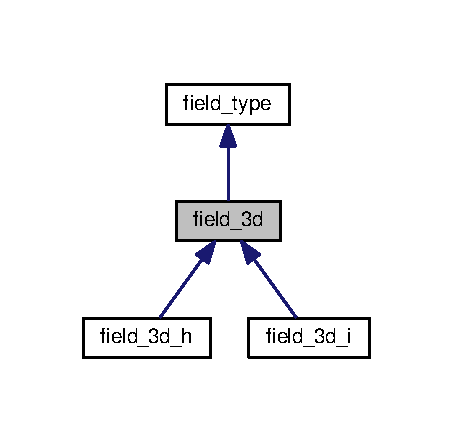
\includegraphics[width=218pt]{d0/d2b/classfield__3d__inherit__graph}
\end{center}
\end{figure}


Collaboration diagram for field\+\_\+3d\+:\nopagebreak
\begin{figure}[H]
\begin{center}
\leavevmode
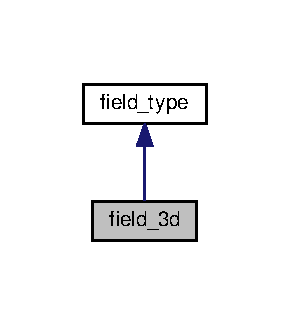
\includegraphics[width=139pt]{d0/d96/classfield__3d__coll__graph}
\end{center}
\end{figure}
\subsection*{Public Member Functions}
\begin{DoxyCompactItemize}
\item 
\hyperlink{classfield__3d_a646422ddfcf4ebd3ebf452f775d353d9}{field\+\_\+3d} ()
\item 
\hyperlink{classfield__3d_ae824f31b4096ae69fe2f116c09e5836e}{$\sim$field\+\_\+3d} ()
\item 
void \hyperlink{classfield__3d_ab7818297f6dbba8842eb8ebcfd8cd234}{next} (bool \&finish, std\+::vector$<$ int $>$ \&pos)
\item 
bool \hyperlink{classfield__3d_a18debdb40fa4de1d676cc64f0c4a9c85}{check\+\_\+zero} (std\+::vector$<$ int $>$ \&position)
\item 
void \hyperlink{classfield__3d_a22fd3cb8126c465128454c96b349ca69}{get\+\_\+3dzero} (bool $\ast$$\ast$$\ast$\&x) const 
\item 
int \hyperlink{classfield__3d_aec848e9158c3d5283791c564baa7e982}{findnum} ()
\end{DoxyCompactItemize}
\subsection*{Protected Attributes}
\begin{DoxyCompactItemize}
\item 
bool $\ast$$\ast$$\ast$ \hyperlink{classfield__3d_a024d0b7a17147d4955337f54078a8c86}{iszero}
\end{DoxyCompactItemize}


\subsection{Constructor \& Destructor Documentation}
\index{field\+\_\+3d@{field\+\_\+3d}!field\+\_\+3d@{field\+\_\+3d}}
\index{field\+\_\+3d@{field\+\_\+3d}!field\+\_\+3d@{field\+\_\+3d}}
\subsubsection[{\texorpdfstring{field\+\_\+3d()}{field_3d()}}]{\setlength{\rightskip}{0pt plus 5cm}field\+\_\+3d\+::field\+\_\+3d (
\begin{DoxyParamCaption}
{}
\end{DoxyParamCaption}
)\hspace{0.3cm}{\ttfamily [inline]}}\hypertarget{classfield__3d_a646422ddfcf4ebd3ebf452f775d353d9}{}\label{classfield__3d_a646422ddfcf4ebd3ebf452f775d353d9}
\index{field\+\_\+3d@{field\+\_\+3d}!````~field\+\_\+3d@{$\sim$field\+\_\+3d}}
\index{````~field\+\_\+3d@{$\sim$field\+\_\+3d}!field\+\_\+3d@{field\+\_\+3d}}
\subsubsection[{\texorpdfstring{$\sim$field\+\_\+3d()}{~field_3d()}}]{\setlength{\rightskip}{0pt plus 5cm}field\+\_\+3d\+::$\sim$field\+\_\+3d (
\begin{DoxyParamCaption}
{}
\end{DoxyParamCaption}
)\hspace{0.3cm}{\ttfamily [inline]}}\hypertarget{classfield__3d_ae824f31b4096ae69fe2f116c09e5836e}{}\label{classfield__3d_ae824f31b4096ae69fe2f116c09e5836e}


\subsection{Member Function Documentation}
\index{field\+\_\+3d@{field\+\_\+3d}!check\+\_\+zero@{check\+\_\+zero}}
\index{check\+\_\+zero@{check\+\_\+zero}!field\+\_\+3d@{field\+\_\+3d}}
\subsubsection[{\texorpdfstring{check\+\_\+zero(std\+::vector$<$ int $>$ \&position)}{check_zero(std::vector< int > &position)}}]{\setlength{\rightskip}{0pt plus 5cm}bool field\+\_\+3d\+::check\+\_\+zero (
\begin{DoxyParamCaption}
\item[{std\+::vector$<$ int $>$ \&}]{position}
\end{DoxyParamCaption}
)\hspace{0.3cm}{\ttfamily [inline]}, {\ttfamily [virtual]}}\hypertarget{classfield__3d_a18debdb40fa4de1d676cc64f0c4a9c85}{}\label{classfield__3d_a18debdb40fa4de1d676cc64f0c4a9c85}


Reimplemented from \hyperlink{classfield__type_a8aabf0f54a8dc73b1ac529a26604c827}{field\+\_\+type}.

\index{field\+\_\+3d@{field\+\_\+3d}!findnum@{findnum}}
\index{findnum@{findnum}!field\+\_\+3d@{field\+\_\+3d}}
\subsubsection[{\texorpdfstring{findnum()}{findnum()}}]{\setlength{\rightskip}{0pt plus 5cm}int field\+\_\+3d\+::findnum (
\begin{DoxyParamCaption}
{}
\end{DoxyParamCaption}
)\hspace{0.3cm}{\ttfamily [virtual]}}\hypertarget{classfield__3d_aec848e9158c3d5283791c564baa7e982}{}\label{classfield__3d_aec848e9158c3d5283791c564baa7e982}


Reimplemented from \hyperlink{classfield__type_a73e5605cfd2714b2a358d61c4b102883}{field\+\_\+type}.

\index{field\+\_\+3d@{field\+\_\+3d}!get\+\_\+3dzero@{get\+\_\+3dzero}}
\index{get\+\_\+3dzero@{get\+\_\+3dzero}!field\+\_\+3d@{field\+\_\+3d}}
\subsubsection[{\texorpdfstring{get\+\_\+3dzero(bool $\ast$$\ast$$\ast$\&x) const }{get_3dzero(bool ***&x) const }}]{\setlength{\rightskip}{0pt plus 5cm}void field\+\_\+3d\+::get\+\_\+3dzero (
\begin{DoxyParamCaption}
\item[{bool $\ast$$\ast$$\ast$\&}]{x}
\end{DoxyParamCaption}
) const\hspace{0.3cm}{\ttfamily [inline]}, {\ttfamily [virtual]}}\hypertarget{classfield__3d_a22fd3cb8126c465128454c96b349ca69}{}\label{classfield__3d_a22fd3cb8126c465128454c96b349ca69}


Reimplemented from \hyperlink{classfield__type_aa6fa2f915583fc2941db7713138d8f8b}{field\+\_\+type}.

\index{field\+\_\+3d@{field\+\_\+3d}!next@{next}}
\index{next@{next}!field\+\_\+3d@{field\+\_\+3d}}
\subsubsection[{\texorpdfstring{next(bool \&finish, std\+::vector$<$ int $>$ \&pos)}{next(bool &finish, std::vector< int > &pos)}}]{\setlength{\rightskip}{0pt plus 5cm}void field\+\_\+3d\+::next (
\begin{DoxyParamCaption}
\item[{bool \&}]{finish, }
\item[{std\+::vector$<$ int $>$ \&}]{pos}
\end{DoxyParamCaption}
)\hspace{0.3cm}{\ttfamily [virtual]}}\hypertarget{classfield__3d_ab7818297f6dbba8842eb8ebcfd8cd234}{}\label{classfield__3d_ab7818297f6dbba8842eb8ebcfd8cd234}


Reimplemented from \hyperlink{classfield__type_afaf4b3449a0ee906ebe543439054eab5}{field\+\_\+type}.



\subsection{Member Data Documentation}
\index{field\+\_\+3d@{field\+\_\+3d}!iszero@{iszero}}
\index{iszero@{iszero}!field\+\_\+3d@{field\+\_\+3d}}
\subsubsection[{\texorpdfstring{iszero}{iszero}}]{\setlength{\rightskip}{0pt plus 5cm}bool$\ast$$\ast$$\ast$ field\+\_\+3d\+::iszero\hspace{0.3cm}{\ttfamily [protected]}}\hypertarget{classfield__3d_a024d0b7a17147d4955337f54078a8c86}{}\label{classfield__3d_a024d0b7a17147d4955337f54078a8c86}


The documentation for this class was generated from the following file\+:\begin{DoxyCompactItemize}
\item 
includes/\hyperlink{field__type_8hpp}{field\+\_\+type.\+hpp}\end{DoxyCompactItemize}

\hypertarget{classfield__3d__h}{}\section{field\+\_\+3d\+\_\+h Class Reference}
\label{classfield__3d__h}\index{field\+\_\+3d\+\_\+h@{field\+\_\+3d\+\_\+h}}


{\ttfamily \#include $<$field\+\_\+type.\+hpp$>$}



Inheritance diagram for field\+\_\+3d\+\_\+h\+:
\nopagebreak
\begin{figure}[H]
\begin{center}
\leavevmode
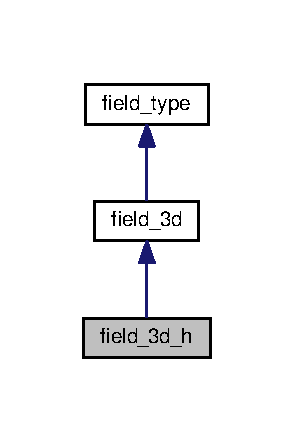
\includegraphics[width=141pt]{d7/d5b/classfield__3d__h__inherit__graph}
\end{center}
\end{figure}


Collaboration diagram for field\+\_\+3d\+\_\+h\+:
\nopagebreak
\begin{figure}[H]
\begin{center}
\leavevmode
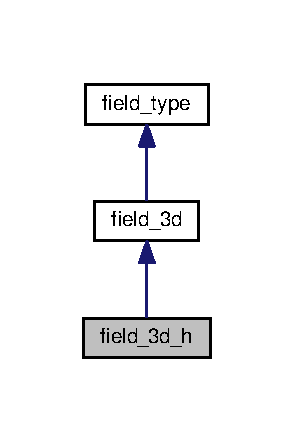
\includegraphics[width=141pt]{dd/d2a/classfield__3d__h__coll__graph}
\end{center}
\end{figure}
\subsection*{Public Member Functions}
\begin{DoxyCompactItemize}
\item 
\hyperlink{classfield__3d__h_ab4075a1ea58d9dfba6593634fc82b581}{field\+\_\+3d\+\_\+h} ()
\item 
\hyperlink{classfield__3d__h_abeec2e1a4d0fa1e38677acb8e459a4e6}{field\+\_\+3d\+\_\+h} (int size, bool isperio)
\item 
\hyperlink{classfield__3d__h_a8f520edb96a4be3b2346b5d6f5fd1799}{field\+\_\+3d\+\_\+h} (int size, bool isperio, int p\+\_\+pad)
\item 
\hyperlink{classfield__3d__h_a3a527e3d3847d7d43d4740c291a558c4}{field\+\_\+3d\+\_\+h} (\hyperlink{classfield__type}{field\+\_\+type} \&other)
\item 
\hyperlink{classfield__3d__h_a57b5974d6f1b3fc85bb8a063224c61e7}{field\+\_\+3d\+\_\+h} (const \hyperlink{classfield__3d__h}{field\+\_\+3d\+\_\+h} \&other)
\item 
\hyperlink{classfield__3d__h_a50fc7168e6083674703fa177e736efe1}{$\sim$field\+\_\+3d\+\_\+h} ()
\item 
void \hyperlink{classfield__3d__h_a2bf31b5938e68787979c41af562cef0e}{h\+\_\+access} (std\+::vector$<$ int $>$ \&position, std\+::vector$<$ double $>$ \&out)
\item 
void \hyperlink{classfield__3d__h_a48336ddd5b0e036bde1db2c324b830bf}{h\+\_\+next} (bool \&finish, std\+::vector$<$ int $>$ \&pos, std\+::vector$<$ double $>$ \&out)
\item 
void \hyperlink{classfield__3d__h_a1591db771816e1dd5b9971463cd14988}{fill\+\_\+ghost} (int num\+\_\+rows)
\item 
\hyperlink{classfield__3d__h}{field\+\_\+3d\+\_\+h} \& \hyperlink{classfield__3d__h_adf1f7a69955404d0ed6a9b647e176d34}{operator=} (const \hyperlink{classfield__3d__h}{field\+\_\+3d\+\_\+h} \&other)
\item 
void \hyperlink{classfield__3d__h_ae28101f8213ae939766b611c2c8116d2}{get\+\_\+3dfield\+\_\+h} (double $\ast$$\ast$$\ast$\&x, double $\ast$$\ast$$\ast$\&y, double $\ast$$\ast$$\ast$\&z) const 
\item 
void \hyperlink{classfield__3d__h_a9ff4a061c1f2c293e1ab8775df1fec1f}{h\+\_\+adjacent} (std\+::vector$<$ int $>$ \&position, double $\ast$$\ast$out)
\item 
void \hyperlink{classfield__3d__h_a0fc4bbb10cd843962516134a199d65a7}{h\+\_\+2adjacent} (std\+::vector$<$ int $>$ \&position, double $\ast$$\ast$out)
\item 
void \hyperlink{classfield__3d__h_a85ce1558d9260abb50dbbf0a210764ba}{fill\+\_\+rand} (std\+::vector$<$ int $>$ \&position)
\item 
void \hyperlink{classfield__3d__h_aa703c9cc42ed4f072e0defce344d4de3}{fill\+\_\+one} (std\+::vector$<$ int $>$ \&position)
\item 
void \hyperlink{classfield__3d__h_acbcafe9fa529695f142a9b352821ecbe}{fill\+\_\+zero} (std\+::vector$<$ int $>$ \&position)
\item 
void \hyperlink{classfield__3d__h_a11e90275cade149683013d09e9dd9756}{fill\+\_\+val\+\_\+h} (std\+::vector$<$ int $>$ \&position, double x, double y, double z)
\item 
void \hyperlink{classfield__3d__h_a90b81a79c986e2b8ec3243a75eec7663}{add\+\_\+val\+\_\+h} (std\+::vector$<$ int $>$ \&position, std\+::vector$<$ double $>$ \&in)
\item 
void \hyperlink{classfield__3d__h_a5bd770e759efdc768af894b3a57a8b90}{change\+\_\+to\+\_\+test} (std\+::vector$<$ int $>$ \&position, \hyperlink{classham__type}{ham\+\_\+type} $\ast$hamil)
\item 
void \hyperlink{classfield__3d__h_a7650e01a5aaf8c9e87f5684f4e9e6040}{h\+\_\+arb\+\_\+adj} (std\+::vector$<$ int $>$ \&position, std\+::vector$<$ int $>$ \&dxs, std\+::vector$<$ int $>$ \&dys, std\+::vector$<$ int $>$ \&dzs, double $\ast$$\ast$out, int num)
\item 
void \hyperlink{classfield__3d__h_a07dd0d01b8281641d9789c46db36f85e}{print} (std\+::string filename, std\+::string arrname)
\item 
void \hyperlink{classfield__3d__h_a7548b12d8552e485ab78bcfd757c90bd}{print\+\_\+setup} (const std\+::string filename, const std\+::string groupname, const int Tmax, const int Hmax)
\item 
void \hyperlink{classfield__3d__h_a81dc2e770a20c56b31ad5ab90575bf42}{send\+\_\+data} (int dest\+\_\+rank)
\item 
void \hyperlink{classfield__3d__h_a75bb987ad328cf6470d8b53575a2cd7e}{recv\+\_\+data} (int src\+\_\+rank)
\end{DoxyCompactItemize}
\subsection*{Protected Attributes}
\begin{DoxyCompactItemize}
\item 
double $\ast$$\ast$$\ast$ \hyperlink{classfield__3d__h_a9555e25d3918c95671b8bf5e54877c65}{spinx}
\item 
double $\ast$$\ast$$\ast$ \hyperlink{classfield__3d__h_a4e077beb71f0e370b1376b98ad9b22c6}{spiny}
\item 
double $\ast$$\ast$$\ast$ \hyperlink{classfield__3d__h_af5df1b887b63dc72f61812aeff434312}{spinz}
\item 
int $\ast$$\ast$ \hyperlink{classfield__3d__h_acc1b62f03c4c546364f12507c8632360}{postemp}
\item 
int \hyperlink{classfield__3d__h_ace62ac7262cac2aeea510f01e18c3176}{dirsx} \mbox{[}6\mbox{]}
\item 
int \hyperlink{classfield__3d__h_a2eb512be62c242bdf64b9675a1073d10}{dirsy} \mbox{[}6\mbox{]}
\item 
int \hyperlink{classfield__3d__h_af9adc2db425114219dbf8180cf8f47fd}{dirsz} \mbox{[}6\mbox{]}
\end{DoxyCompactItemize}


\subsection{Constructor \& Destructor Documentation}
\index{field\+\_\+3d\+\_\+h@{field\+\_\+3d\+\_\+h}!field\+\_\+3d\+\_\+h@{field\+\_\+3d\+\_\+h}}
\index{field\+\_\+3d\+\_\+h@{field\+\_\+3d\+\_\+h}!field\+\_\+3d\+\_\+h@{field\+\_\+3d\+\_\+h}}
\subsubsection[{\texorpdfstring{field\+\_\+3d\+\_\+h()}{field_3d_h()}}]{\setlength{\rightskip}{0pt plus 5cm}field\+\_\+3d\+\_\+h\+::field\+\_\+3d\+\_\+h (
\begin{DoxyParamCaption}
{}
\end{DoxyParamCaption}
)}\hypertarget{classfield__3d__h_ab4075a1ea58d9dfba6593634fc82b581}{}\label{classfield__3d__h_ab4075a1ea58d9dfba6593634fc82b581}
\index{field\+\_\+3d\+\_\+h@{field\+\_\+3d\+\_\+h}!field\+\_\+3d\+\_\+h@{field\+\_\+3d\+\_\+h}}
\index{field\+\_\+3d\+\_\+h@{field\+\_\+3d\+\_\+h}!field\+\_\+3d\+\_\+h@{field\+\_\+3d\+\_\+h}}
\subsubsection[{\texorpdfstring{field\+\_\+3d\+\_\+h(int size, bool isperio)}{field_3d_h(int size, bool isperio)}}]{\setlength{\rightskip}{0pt plus 5cm}field\+\_\+3d\+\_\+h\+::field\+\_\+3d\+\_\+h (
\begin{DoxyParamCaption}
\item[{int}]{size, }
\item[{bool}]{isperio}
\end{DoxyParamCaption}
)}\hypertarget{classfield__3d__h_abeec2e1a4d0fa1e38677acb8e459a4e6}{}\label{classfield__3d__h_abeec2e1a4d0fa1e38677acb8e459a4e6}
\index{field\+\_\+3d\+\_\+h@{field\+\_\+3d\+\_\+h}!field\+\_\+3d\+\_\+h@{field\+\_\+3d\+\_\+h}}
\index{field\+\_\+3d\+\_\+h@{field\+\_\+3d\+\_\+h}!field\+\_\+3d\+\_\+h@{field\+\_\+3d\+\_\+h}}
\subsubsection[{\texorpdfstring{field\+\_\+3d\+\_\+h(int size, bool isperio, int p\+\_\+pad)}{field_3d_h(int size, bool isperio, int p_pad)}}]{\setlength{\rightskip}{0pt plus 5cm}field\+\_\+3d\+\_\+h\+::field\+\_\+3d\+\_\+h (
\begin{DoxyParamCaption}
\item[{int}]{size, }
\item[{bool}]{isperio, }
\item[{int}]{p\+\_\+pad}
\end{DoxyParamCaption}
)}\hypertarget{classfield__3d__h_a8f520edb96a4be3b2346b5d6f5fd1799}{}\label{classfield__3d__h_a8f520edb96a4be3b2346b5d6f5fd1799}
\index{field\+\_\+3d\+\_\+h@{field\+\_\+3d\+\_\+h}!field\+\_\+3d\+\_\+h@{field\+\_\+3d\+\_\+h}}
\index{field\+\_\+3d\+\_\+h@{field\+\_\+3d\+\_\+h}!field\+\_\+3d\+\_\+h@{field\+\_\+3d\+\_\+h}}
\subsubsection[{\texorpdfstring{field\+\_\+3d\+\_\+h(field\+\_\+type \&other)}{field_3d_h(field_type &other)}}]{\setlength{\rightskip}{0pt plus 5cm}field\+\_\+3d\+\_\+h\+::field\+\_\+3d\+\_\+h (
\begin{DoxyParamCaption}
\item[{{\bf field\+\_\+type} \&}]{other}
\end{DoxyParamCaption}
)}\hypertarget{classfield__3d__h_a3a527e3d3847d7d43d4740c291a558c4}{}\label{classfield__3d__h_a3a527e3d3847d7d43d4740c291a558c4}
\index{field\+\_\+3d\+\_\+h@{field\+\_\+3d\+\_\+h}!field\+\_\+3d\+\_\+h@{field\+\_\+3d\+\_\+h}}
\index{field\+\_\+3d\+\_\+h@{field\+\_\+3d\+\_\+h}!field\+\_\+3d\+\_\+h@{field\+\_\+3d\+\_\+h}}
\subsubsection[{\texorpdfstring{field\+\_\+3d\+\_\+h(const field\+\_\+3d\+\_\+h \&other)}{field_3d_h(const field_3d_h &other)}}]{\setlength{\rightskip}{0pt plus 5cm}field\+\_\+3d\+\_\+h\+::field\+\_\+3d\+\_\+h (
\begin{DoxyParamCaption}
\item[{const {\bf field\+\_\+3d\+\_\+h} \&}]{other}
\end{DoxyParamCaption}
)}\hypertarget{classfield__3d__h_a57b5974d6f1b3fc85bb8a063224c61e7}{}\label{classfield__3d__h_a57b5974d6f1b3fc85bb8a063224c61e7}
\index{field\+\_\+3d\+\_\+h@{field\+\_\+3d\+\_\+h}!````~field\+\_\+3d\+\_\+h@{$\sim$field\+\_\+3d\+\_\+h}}
\index{````~field\+\_\+3d\+\_\+h@{$\sim$field\+\_\+3d\+\_\+h}!field\+\_\+3d\+\_\+h@{field\+\_\+3d\+\_\+h}}
\subsubsection[{\texorpdfstring{$\sim$field\+\_\+3d\+\_\+h()}{~field_3d_h()}}]{\setlength{\rightskip}{0pt plus 5cm}field\+\_\+3d\+\_\+h\+::$\sim$field\+\_\+3d\+\_\+h (
\begin{DoxyParamCaption}
{}
\end{DoxyParamCaption}
)}\hypertarget{classfield__3d__h_a50fc7168e6083674703fa177e736efe1}{}\label{classfield__3d__h_a50fc7168e6083674703fa177e736efe1}


\subsection{Member Function Documentation}
\index{field\+\_\+3d\+\_\+h@{field\+\_\+3d\+\_\+h}!add\+\_\+val\+\_\+h@{add\+\_\+val\+\_\+h}}
\index{add\+\_\+val\+\_\+h@{add\+\_\+val\+\_\+h}!field\+\_\+3d\+\_\+h@{field\+\_\+3d\+\_\+h}}
\subsubsection[{\texorpdfstring{add\+\_\+val\+\_\+h(std\+::vector$<$ int $>$ \&position, std\+::vector$<$ double $>$ \&in)}{add_val_h(std::vector< int > &position, std::vector< double > &in)}}]{\setlength{\rightskip}{0pt plus 5cm}void field\+\_\+3d\+\_\+h\+::add\+\_\+val\+\_\+h (
\begin{DoxyParamCaption}
\item[{std\+::vector$<$ int $>$ \&}]{position, }
\item[{std\+::vector$<$ double $>$ \&}]{in}
\end{DoxyParamCaption}
)\hspace{0.3cm}{\ttfamily [virtual]}}\hypertarget{classfield__3d__h_a90b81a79c986e2b8ec3243a75eec7663}{}\label{classfield__3d__h_a90b81a79c986e2b8ec3243a75eec7663}


Reimplemented from \hyperlink{classfield__type_a35a20297e1cddac40d4c2aecef5a5594}{field\+\_\+type}.

\index{field\+\_\+3d\+\_\+h@{field\+\_\+3d\+\_\+h}!change\+\_\+to\+\_\+test@{change\+\_\+to\+\_\+test}}
\index{change\+\_\+to\+\_\+test@{change\+\_\+to\+\_\+test}!field\+\_\+3d\+\_\+h@{field\+\_\+3d\+\_\+h}}
\subsubsection[{\texorpdfstring{change\+\_\+to\+\_\+test(std\+::vector$<$ int $>$ \&position, ham\+\_\+type $\ast$hamil)}{change_to_test(std::vector< int > &position, ham_type *hamil)}}]{\setlength{\rightskip}{0pt plus 5cm}void field\+\_\+3d\+\_\+h\+::change\+\_\+to\+\_\+test (
\begin{DoxyParamCaption}
\item[{std\+::vector$<$ int $>$ \&}]{position, }
\item[{{\bf ham\+\_\+type} $\ast$}]{hamil}
\end{DoxyParamCaption}
)\hspace{0.3cm}{\ttfamily [virtual]}}\hypertarget{classfield__3d__h_a5bd770e759efdc768af894b3a57a8b90}{}\label{classfield__3d__h_a5bd770e759efdc768af894b3a57a8b90}


Reimplemented from \hyperlink{classfield__type_a32140b8a785c0139dd27304143ca5f17}{field\+\_\+type}.

\index{field\+\_\+3d\+\_\+h@{field\+\_\+3d\+\_\+h}!fill\+\_\+ghost@{fill\+\_\+ghost}}
\index{fill\+\_\+ghost@{fill\+\_\+ghost}!field\+\_\+3d\+\_\+h@{field\+\_\+3d\+\_\+h}}
\subsubsection[{\texorpdfstring{fill\+\_\+ghost(int num\+\_\+rows)}{fill_ghost(int num_rows)}}]{\setlength{\rightskip}{0pt plus 5cm}void field\+\_\+3d\+\_\+h\+::fill\+\_\+ghost (
\begin{DoxyParamCaption}
\item[{int}]{num\+\_\+rows}
\end{DoxyParamCaption}
)\hspace{0.3cm}{\ttfamily [virtual]}}\hypertarget{classfield__3d__h_a1591db771816e1dd5b9971463cd14988}{}\label{classfield__3d__h_a1591db771816e1dd5b9971463cd14988}


Reimplemented from \hyperlink{classfield__type_a11c23271c828983406e8e80c66b81c46}{field\+\_\+type}.

\index{field\+\_\+3d\+\_\+h@{field\+\_\+3d\+\_\+h}!fill\+\_\+one@{fill\+\_\+one}}
\index{fill\+\_\+one@{fill\+\_\+one}!field\+\_\+3d\+\_\+h@{field\+\_\+3d\+\_\+h}}
\subsubsection[{\texorpdfstring{fill\+\_\+one(std\+::vector$<$ int $>$ \&position)}{fill_one(std::vector< int > &position)}}]{\setlength{\rightskip}{0pt plus 5cm}void field\+\_\+3d\+\_\+h\+::fill\+\_\+one (
\begin{DoxyParamCaption}
\item[{std\+::vector$<$ int $>$ \&}]{position}
\end{DoxyParamCaption}
)\hspace{0.3cm}{\ttfamily [virtual]}}\hypertarget{classfield__3d__h_aa703c9cc42ed4f072e0defce344d4de3}{}\label{classfield__3d__h_aa703c9cc42ed4f072e0defce344d4de3}


Reimplemented from \hyperlink{classfield__type_acb4fb5c3393feed8685eb3957c032a15}{field\+\_\+type}.

\index{field\+\_\+3d\+\_\+h@{field\+\_\+3d\+\_\+h}!fill\+\_\+rand@{fill\+\_\+rand}}
\index{fill\+\_\+rand@{fill\+\_\+rand}!field\+\_\+3d\+\_\+h@{field\+\_\+3d\+\_\+h}}
\subsubsection[{\texorpdfstring{fill\+\_\+rand(std\+::vector$<$ int $>$ \&position)}{fill_rand(std::vector< int > &position)}}]{\setlength{\rightskip}{0pt plus 5cm}void field\+\_\+3d\+\_\+h\+::fill\+\_\+rand (
\begin{DoxyParamCaption}
\item[{std\+::vector$<$ int $>$ \&}]{position}
\end{DoxyParamCaption}
)\hspace{0.3cm}{\ttfamily [virtual]}}\hypertarget{classfield__3d__h_a85ce1558d9260abb50dbbf0a210764ba}{}\label{classfield__3d__h_a85ce1558d9260abb50dbbf0a210764ba}


Reimplemented from \hyperlink{classfield__type_a87d6bf8e9e97ce158a356fefaddc3bee}{field\+\_\+type}.

\index{field\+\_\+3d\+\_\+h@{field\+\_\+3d\+\_\+h}!fill\+\_\+val\+\_\+h@{fill\+\_\+val\+\_\+h}}
\index{fill\+\_\+val\+\_\+h@{fill\+\_\+val\+\_\+h}!field\+\_\+3d\+\_\+h@{field\+\_\+3d\+\_\+h}}
\subsubsection[{\texorpdfstring{fill\+\_\+val\+\_\+h(std\+::vector$<$ int $>$ \&position, double x, double y, double z)}{fill_val_h(std::vector< int > &position, double x, double y, double z)}}]{\setlength{\rightskip}{0pt plus 5cm}void field\+\_\+3d\+\_\+h\+::fill\+\_\+val\+\_\+h (
\begin{DoxyParamCaption}
\item[{std\+::vector$<$ int $>$ \&}]{position, }
\item[{double}]{x, }
\item[{double}]{y, }
\item[{double}]{z}
\end{DoxyParamCaption}
)\hspace{0.3cm}{\ttfamily [virtual]}}\hypertarget{classfield__3d__h_a11e90275cade149683013d09e9dd9756}{}\label{classfield__3d__h_a11e90275cade149683013d09e9dd9756}


Reimplemented from \hyperlink{classfield__type_a02500bfb9021cf13ff6e1be66b63b9ae}{field\+\_\+type}.

\index{field\+\_\+3d\+\_\+h@{field\+\_\+3d\+\_\+h}!fill\+\_\+zero@{fill\+\_\+zero}}
\index{fill\+\_\+zero@{fill\+\_\+zero}!field\+\_\+3d\+\_\+h@{field\+\_\+3d\+\_\+h}}
\subsubsection[{\texorpdfstring{fill\+\_\+zero(std\+::vector$<$ int $>$ \&position)}{fill_zero(std::vector< int > &position)}}]{\setlength{\rightskip}{0pt plus 5cm}void field\+\_\+3d\+\_\+h\+::fill\+\_\+zero (
\begin{DoxyParamCaption}
\item[{std\+::vector$<$ int $>$ \&}]{position}
\end{DoxyParamCaption}
)\hspace{0.3cm}{\ttfamily [virtual]}}\hypertarget{classfield__3d__h_acbcafe9fa529695f142a9b352821ecbe}{}\label{classfield__3d__h_acbcafe9fa529695f142a9b352821ecbe}


Reimplemented from \hyperlink{classfield__type_afdb5b29e839fa11c7faeff60ee49aebb}{field\+\_\+type}.

\index{field\+\_\+3d\+\_\+h@{field\+\_\+3d\+\_\+h}!get\+\_\+3dfield\+\_\+h@{get\+\_\+3dfield\+\_\+h}}
\index{get\+\_\+3dfield\+\_\+h@{get\+\_\+3dfield\+\_\+h}!field\+\_\+3d\+\_\+h@{field\+\_\+3d\+\_\+h}}
\subsubsection[{\texorpdfstring{get\+\_\+3dfield\+\_\+h(double $\ast$$\ast$$\ast$\&x, double $\ast$$\ast$$\ast$\&y, double $\ast$$\ast$$\ast$\&z) const }{get_3dfield_h(double ***&x, double ***&y, double ***&z) const }}]{\setlength{\rightskip}{0pt plus 5cm}void field\+\_\+3d\+\_\+h\+::get\+\_\+3dfield\+\_\+h (
\begin{DoxyParamCaption}
\item[{double $\ast$$\ast$$\ast$\&}]{x, }
\item[{double $\ast$$\ast$$\ast$\&}]{y, }
\item[{double $\ast$$\ast$$\ast$\&}]{z}
\end{DoxyParamCaption}
) const\hspace{0.3cm}{\ttfamily [virtual]}}\hypertarget{classfield__3d__h_ae28101f8213ae939766b611c2c8116d2}{}\label{classfield__3d__h_ae28101f8213ae939766b611c2c8116d2}


Reimplemented from \hyperlink{classfield__type_ae8649f8841a9c363914d4f72cea4df5f}{field\+\_\+type}.

\index{field\+\_\+3d\+\_\+h@{field\+\_\+3d\+\_\+h}!h\+\_\+2adjacent@{h\+\_\+2adjacent}}
\index{h\+\_\+2adjacent@{h\+\_\+2adjacent}!field\+\_\+3d\+\_\+h@{field\+\_\+3d\+\_\+h}}
\subsubsection[{\texorpdfstring{h\+\_\+2adjacent(std\+::vector$<$ int $>$ \&position, double $\ast$$\ast$out)}{h_2adjacent(std::vector< int > &position, double **out)}}]{\setlength{\rightskip}{0pt plus 5cm}void field\+\_\+3d\+\_\+h\+::h\+\_\+2adjacent (
\begin{DoxyParamCaption}
\item[{std\+::vector$<$ int $>$ \&}]{position, }
\item[{double $\ast$$\ast$}]{out}
\end{DoxyParamCaption}
)\hspace{0.3cm}{\ttfamily [virtual]}}\hypertarget{classfield__3d__h_a0fc4bbb10cd843962516134a199d65a7}{}\label{classfield__3d__h_a0fc4bbb10cd843962516134a199d65a7}


Reimplemented from \hyperlink{classfield__type_a77964e0d6f8d20c9a1ec579847570c4c}{field\+\_\+type}.

\index{field\+\_\+3d\+\_\+h@{field\+\_\+3d\+\_\+h}!h\+\_\+access@{h\+\_\+access}}
\index{h\+\_\+access@{h\+\_\+access}!field\+\_\+3d\+\_\+h@{field\+\_\+3d\+\_\+h}}
\subsubsection[{\texorpdfstring{h\+\_\+access(std\+::vector$<$ int $>$ \&position, std\+::vector$<$ double $>$ \&out)}{h_access(std::vector< int > &position, std::vector< double > &out)}}]{\setlength{\rightskip}{0pt plus 5cm}void field\+\_\+3d\+\_\+h\+::h\+\_\+access (
\begin{DoxyParamCaption}
\item[{std\+::vector$<$ int $>$ \&}]{position, }
\item[{std\+::vector$<$ double $>$ \&}]{out}
\end{DoxyParamCaption}
)\hspace{0.3cm}{\ttfamily [virtual]}}\hypertarget{classfield__3d__h_a2bf31b5938e68787979c41af562cef0e}{}\label{classfield__3d__h_a2bf31b5938e68787979c41af562cef0e}


Reimplemented from \hyperlink{classfield__type_ada65523f1a000cbd929f2d97d747fa59}{field\+\_\+type}.

\index{field\+\_\+3d\+\_\+h@{field\+\_\+3d\+\_\+h}!h\+\_\+adjacent@{h\+\_\+adjacent}}
\index{h\+\_\+adjacent@{h\+\_\+adjacent}!field\+\_\+3d\+\_\+h@{field\+\_\+3d\+\_\+h}}
\subsubsection[{\texorpdfstring{h\+\_\+adjacent(std\+::vector$<$ int $>$ \&position, double $\ast$$\ast$out)}{h_adjacent(std::vector< int > &position, double **out)}}]{\setlength{\rightskip}{0pt plus 5cm}void field\+\_\+3d\+\_\+h\+::h\+\_\+adjacent (
\begin{DoxyParamCaption}
\item[{std\+::vector$<$ int $>$ \&}]{position, }
\item[{double $\ast$$\ast$}]{out}
\end{DoxyParamCaption}
)\hspace{0.3cm}{\ttfamily [virtual]}}\hypertarget{classfield__3d__h_a9ff4a061c1f2c293e1ab8775df1fec1f}{}\label{classfield__3d__h_a9ff4a061c1f2c293e1ab8775df1fec1f}


Reimplemented from \hyperlink{classfield__type_af91a0a4b7d3076c41baa96f25faec0c4}{field\+\_\+type}.

\index{field\+\_\+3d\+\_\+h@{field\+\_\+3d\+\_\+h}!h\+\_\+arb\+\_\+adj@{h\+\_\+arb\+\_\+adj}}
\index{h\+\_\+arb\+\_\+adj@{h\+\_\+arb\+\_\+adj}!field\+\_\+3d\+\_\+h@{field\+\_\+3d\+\_\+h}}
\subsubsection[{\texorpdfstring{h\+\_\+arb\+\_\+adj(std\+::vector$<$ int $>$ \&position, std\+::vector$<$ int $>$ \&dxs, std\+::vector$<$ int $>$ \&dys, std\+::vector$<$ int $>$ \&dzs, double $\ast$$\ast$out, int num)}{h_arb_adj(std::vector< int > &position, std::vector< int > &dxs, std::vector< int > &dys, std::vector< int > &dzs, double **out, int num)}}]{\setlength{\rightskip}{0pt plus 5cm}void field\+\_\+3d\+\_\+h\+::h\+\_\+arb\+\_\+adj (
\begin{DoxyParamCaption}
\item[{std\+::vector$<$ int $>$ \&}]{position, }
\item[{std\+::vector$<$ int $>$ \&}]{dxs, }
\item[{std\+::vector$<$ int $>$ \&}]{dys, }
\item[{std\+::vector$<$ int $>$ \&}]{dzs, }
\item[{double $\ast$$\ast$}]{out, }
\item[{int}]{num}
\end{DoxyParamCaption}
)\hspace{0.3cm}{\ttfamily [virtual]}}\hypertarget{classfield__3d__h_a7650e01a5aaf8c9e87f5684f4e9e6040}{}\label{classfield__3d__h_a7650e01a5aaf8c9e87f5684f4e9e6040}


Reimplemented from \hyperlink{classfield__type_a293169a5ca7f03b818c0aa92410a5078}{field\+\_\+type}.

\index{field\+\_\+3d\+\_\+h@{field\+\_\+3d\+\_\+h}!h\+\_\+next@{h\+\_\+next}}
\index{h\+\_\+next@{h\+\_\+next}!field\+\_\+3d\+\_\+h@{field\+\_\+3d\+\_\+h}}
\subsubsection[{\texorpdfstring{h\+\_\+next(bool \&finish, std\+::vector$<$ int $>$ \&pos, std\+::vector$<$ double $>$ \&out)}{h_next(bool &finish, std::vector< int > &pos, std::vector< double > &out)}}]{\setlength{\rightskip}{0pt plus 5cm}void field\+\_\+3d\+\_\+h\+::h\+\_\+next (
\begin{DoxyParamCaption}
\item[{bool \&}]{finish, }
\item[{std\+::vector$<$ int $>$ \&}]{pos, }
\item[{std\+::vector$<$ double $>$ \&}]{out}
\end{DoxyParamCaption}
)\hspace{0.3cm}{\ttfamily [virtual]}}\hypertarget{classfield__3d__h_a48336ddd5b0e036bde1db2c324b830bf}{}\label{classfield__3d__h_a48336ddd5b0e036bde1db2c324b830bf}


Reimplemented from \hyperlink{classfield__type_a4f68c166bbd86806584f44c6d6faf50f}{field\+\_\+type}.

\index{field\+\_\+3d\+\_\+h@{field\+\_\+3d\+\_\+h}!operator=@{operator=}}
\index{operator=@{operator=}!field\+\_\+3d\+\_\+h@{field\+\_\+3d\+\_\+h}}
\subsubsection[{\texorpdfstring{operator=(const field\+\_\+3d\+\_\+h \&other)}{operator=(const field_3d_h &other)}}]{\setlength{\rightskip}{0pt plus 5cm}{\bf field\+\_\+3d\+\_\+h}\& field\+\_\+3d\+\_\+h\+::operator= (
\begin{DoxyParamCaption}
\item[{const {\bf field\+\_\+3d\+\_\+h} \&}]{other}
\end{DoxyParamCaption}
)}\hypertarget{classfield__3d__h_adf1f7a69955404d0ed6a9b647e176d34}{}\label{classfield__3d__h_adf1f7a69955404d0ed6a9b647e176d34}
\index{field\+\_\+3d\+\_\+h@{field\+\_\+3d\+\_\+h}!print@{print}}
\index{print@{print}!field\+\_\+3d\+\_\+h@{field\+\_\+3d\+\_\+h}}
\subsubsection[{\texorpdfstring{print(std\+::string filename, std\+::string arrname)}{print(std::string filename, std::string arrname)}}]{\setlength{\rightskip}{0pt plus 5cm}void field\+\_\+3d\+\_\+h\+::print (
\begin{DoxyParamCaption}
\item[{std\+::string}]{filename, }
\item[{std\+::string}]{arrname}
\end{DoxyParamCaption}
)\hspace{0.3cm}{\ttfamily [virtual]}}\hypertarget{classfield__3d__h_a07dd0d01b8281641d9789c46db36f85e}{}\label{classfield__3d__h_a07dd0d01b8281641d9789c46db36f85e}


Reimplemented from \hyperlink{classfield__type_a70fd2b76f1a1bf1604bcdb39d99687d2}{field\+\_\+type}.

\index{field\+\_\+3d\+\_\+h@{field\+\_\+3d\+\_\+h}!print\+\_\+setup@{print\+\_\+setup}}
\index{print\+\_\+setup@{print\+\_\+setup}!field\+\_\+3d\+\_\+h@{field\+\_\+3d\+\_\+h}}
\subsubsection[{\texorpdfstring{print\+\_\+setup(const std\+::string filename, const std\+::string groupname, const int Tmax, const int Hmax)}{print_setup(const std::string filename, const std::string groupname, const int Tmax, const int Hmax)}}]{\setlength{\rightskip}{0pt plus 5cm}void field\+\_\+3d\+\_\+h\+::print\+\_\+setup (
\begin{DoxyParamCaption}
\item[{const std\+::string}]{filename, }
\item[{const std\+::string}]{groupname, }
\item[{const int}]{Tmax, }
\item[{const int}]{Hmax}
\end{DoxyParamCaption}
)\hspace{0.3cm}{\ttfamily [virtual]}}\hypertarget{classfield__3d__h_a7548b12d8552e485ab78bcfd757c90bd}{}\label{classfield__3d__h_a7548b12d8552e485ab78bcfd757c90bd}


Reimplemented from \hyperlink{classfield__type_a1429809586fadd4afa829bef77fa819d}{field\+\_\+type}.

\index{field\+\_\+3d\+\_\+h@{field\+\_\+3d\+\_\+h}!recv\+\_\+data@{recv\+\_\+data}}
\index{recv\+\_\+data@{recv\+\_\+data}!field\+\_\+3d\+\_\+h@{field\+\_\+3d\+\_\+h}}
\subsubsection[{\texorpdfstring{recv\+\_\+data(int src\+\_\+rank)}{recv_data(int src_rank)}}]{\setlength{\rightskip}{0pt plus 5cm}void field\+\_\+3d\+\_\+h\+::recv\+\_\+data (
\begin{DoxyParamCaption}
\item[{int}]{src\+\_\+rank}
\end{DoxyParamCaption}
)\hspace{0.3cm}{\ttfamily [virtual]}}\hypertarget{classfield__3d__h_a75bb987ad328cf6470d8b53575a2cd7e}{}\label{classfield__3d__h_a75bb987ad328cf6470d8b53575a2cd7e}


Reimplemented from \hyperlink{classfield__type_ac29bf02760384b80a08e5e57ca43542f}{field\+\_\+type}.

\index{field\+\_\+3d\+\_\+h@{field\+\_\+3d\+\_\+h}!send\+\_\+data@{send\+\_\+data}}
\index{send\+\_\+data@{send\+\_\+data}!field\+\_\+3d\+\_\+h@{field\+\_\+3d\+\_\+h}}
\subsubsection[{\texorpdfstring{send\+\_\+data(int dest\+\_\+rank)}{send_data(int dest_rank)}}]{\setlength{\rightskip}{0pt plus 5cm}void field\+\_\+3d\+\_\+h\+::send\+\_\+data (
\begin{DoxyParamCaption}
\item[{int}]{dest\+\_\+rank}
\end{DoxyParamCaption}
)\hspace{0.3cm}{\ttfamily [virtual]}}\hypertarget{classfield__3d__h_a81dc2e770a20c56b31ad5ab90575bf42}{}\label{classfield__3d__h_a81dc2e770a20c56b31ad5ab90575bf42}


Reimplemented from \hyperlink{classfield__type_afaabc410e2ce254c23e3c4aa39d1916d}{field\+\_\+type}.



\subsection{Member Data Documentation}
\index{field\+\_\+3d\+\_\+h@{field\+\_\+3d\+\_\+h}!dirsx@{dirsx}}
\index{dirsx@{dirsx}!field\+\_\+3d\+\_\+h@{field\+\_\+3d\+\_\+h}}
\subsubsection[{\texorpdfstring{dirsx}{dirsx}}]{\setlength{\rightskip}{0pt plus 5cm}int field\+\_\+3d\+\_\+h\+::dirsx\mbox{[}6\mbox{]}\hspace{0.3cm}{\ttfamily [protected]}}\hypertarget{classfield__3d__h_ace62ac7262cac2aeea510f01e18c3176}{}\label{classfield__3d__h_ace62ac7262cac2aeea510f01e18c3176}
\index{field\+\_\+3d\+\_\+h@{field\+\_\+3d\+\_\+h}!dirsy@{dirsy}}
\index{dirsy@{dirsy}!field\+\_\+3d\+\_\+h@{field\+\_\+3d\+\_\+h}}
\subsubsection[{\texorpdfstring{dirsy}{dirsy}}]{\setlength{\rightskip}{0pt plus 5cm}int field\+\_\+3d\+\_\+h\+::dirsy\mbox{[}6\mbox{]}\hspace{0.3cm}{\ttfamily [protected]}}\hypertarget{classfield__3d__h_a2eb512be62c242bdf64b9675a1073d10}{}\label{classfield__3d__h_a2eb512be62c242bdf64b9675a1073d10}
\index{field\+\_\+3d\+\_\+h@{field\+\_\+3d\+\_\+h}!dirsz@{dirsz}}
\index{dirsz@{dirsz}!field\+\_\+3d\+\_\+h@{field\+\_\+3d\+\_\+h}}
\subsubsection[{\texorpdfstring{dirsz}{dirsz}}]{\setlength{\rightskip}{0pt plus 5cm}int field\+\_\+3d\+\_\+h\+::dirsz\mbox{[}6\mbox{]}\hspace{0.3cm}{\ttfamily [protected]}}\hypertarget{classfield__3d__h_af9adc2db425114219dbf8180cf8f47fd}{}\label{classfield__3d__h_af9adc2db425114219dbf8180cf8f47fd}
\index{field\+\_\+3d\+\_\+h@{field\+\_\+3d\+\_\+h}!postemp@{postemp}}
\index{postemp@{postemp}!field\+\_\+3d\+\_\+h@{field\+\_\+3d\+\_\+h}}
\subsubsection[{\texorpdfstring{postemp}{postemp}}]{\setlength{\rightskip}{0pt plus 5cm}int$\ast$$\ast$ field\+\_\+3d\+\_\+h\+::postemp\hspace{0.3cm}{\ttfamily [protected]}}\hypertarget{classfield__3d__h_acc1b62f03c4c546364f12507c8632360}{}\label{classfield__3d__h_acc1b62f03c4c546364f12507c8632360}
\index{field\+\_\+3d\+\_\+h@{field\+\_\+3d\+\_\+h}!spinx@{spinx}}
\index{spinx@{spinx}!field\+\_\+3d\+\_\+h@{field\+\_\+3d\+\_\+h}}
\subsubsection[{\texorpdfstring{spinx}{spinx}}]{\setlength{\rightskip}{0pt plus 5cm}double$\ast$$\ast$$\ast$ field\+\_\+3d\+\_\+h\+::spinx\hspace{0.3cm}{\ttfamily [protected]}}\hypertarget{classfield__3d__h_a9555e25d3918c95671b8bf5e54877c65}{}\label{classfield__3d__h_a9555e25d3918c95671b8bf5e54877c65}
\index{field\+\_\+3d\+\_\+h@{field\+\_\+3d\+\_\+h}!spiny@{spiny}}
\index{spiny@{spiny}!field\+\_\+3d\+\_\+h@{field\+\_\+3d\+\_\+h}}
\subsubsection[{\texorpdfstring{spiny}{spiny}}]{\setlength{\rightskip}{0pt plus 5cm}double$\ast$$\ast$$\ast$ field\+\_\+3d\+\_\+h\+::spiny\hspace{0.3cm}{\ttfamily [protected]}}\hypertarget{classfield__3d__h_a4e077beb71f0e370b1376b98ad9b22c6}{}\label{classfield__3d__h_a4e077beb71f0e370b1376b98ad9b22c6}
\index{field\+\_\+3d\+\_\+h@{field\+\_\+3d\+\_\+h}!spinz@{spinz}}
\index{spinz@{spinz}!field\+\_\+3d\+\_\+h@{field\+\_\+3d\+\_\+h}}
\subsubsection[{\texorpdfstring{spinz}{spinz}}]{\setlength{\rightskip}{0pt plus 5cm}double$\ast$$\ast$$\ast$ field\+\_\+3d\+\_\+h\+::spinz\hspace{0.3cm}{\ttfamily [protected]}}\hypertarget{classfield__3d__h_af5df1b887b63dc72f61812aeff434312}{}\label{classfield__3d__h_af5df1b887b63dc72f61812aeff434312}


The documentation for this class was generated from the following file\+:\begin{DoxyCompactItemize}
\item 
includes/\hyperlink{field__type_8hpp}{field\+\_\+type.\+hpp}\end{DoxyCompactItemize}

\hypertarget{classfield__3d__i}{}\section{field\+\_\+3d\+\_\+i Class Reference}
\label{classfield__3d__i}\index{field\+\_\+3d\+\_\+i@{field\+\_\+3d\+\_\+i}}


{\ttfamily \#include $<$field\+\_\+type.\+hpp$>$}



Inheritance diagram for field\+\_\+3d\+\_\+i\+:
\nopagebreak
\begin{figure}[H]
\begin{center}
\leavevmode
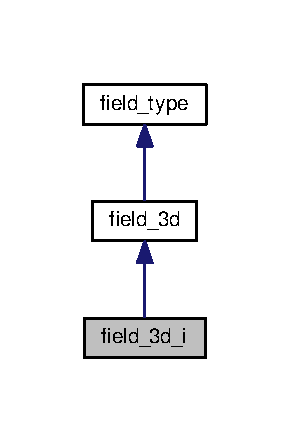
\includegraphics[width=139pt]{db/d8f/classfield__3d__i__inherit__graph}
\end{center}
\end{figure}


Collaboration diagram for field\+\_\+3d\+\_\+i\+:
\nopagebreak
\begin{figure}[H]
\begin{center}
\leavevmode
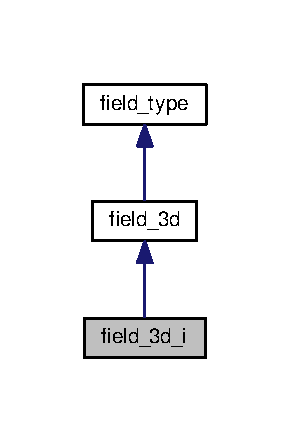
\includegraphics[width=139pt]{dd/ddc/classfield__3d__i__coll__graph}
\end{center}
\end{figure}
\subsection*{Public Member Functions}
\begin{DoxyCompactItemize}
\item 
\hyperlink{classfield__3d__i_a1100cc58d17fcd3edc299d7fb3827b52}{field\+\_\+3d\+\_\+i} ()
\item 
\hyperlink{classfield__3d__i_aa4581cb848c05c9f0492cab5890a706b}{field\+\_\+3d\+\_\+i} (int size, bool isperio)
\item 
\hyperlink{classfield__3d__i_a66200c76ee712977025a7f69d66c375c}{field\+\_\+3d\+\_\+i} (\hyperlink{classfield__type}{field\+\_\+type} \&other)
\item 
\hyperlink{classfield__3d__i_afa1312b43ab3aa34685d4bf5a0d5ce9a}{field\+\_\+3d\+\_\+i} (const \hyperlink{classfield__3d__i}{field\+\_\+3d\+\_\+i} \&other)
\item 
\hyperlink{classfield__3d__i_a34b2bea2d2d2375cafb18a42963e037d}{$\sim$field\+\_\+3d\+\_\+i} ()
\item 
void \hyperlink{classfield__3d__i_abe65be5385f05e22ae373414113229bf}{i\+\_\+access} (std\+::vector$<$ int $>$ \&position, int \&out)
\item 
void \hyperlink{classfield__3d__i_a5cd3d146e8596ab6894f3f64bdad66e7}{i\+\_\+next} (bool \&finish, std\+::vector$<$ int $>$ \&pos, int \&out)
\item 
void \hyperlink{classfield__3d__i_a5c7a0ce8daedd401bdd8c6c57bd5343c}{fill\+\_\+ghost} (int num\+\_\+rows)
\item 
\hyperlink{classfield__3d__i}{field\+\_\+3d\+\_\+i} \& \hyperlink{classfield__3d__i_a1f8a8ea350fcc5c653655fde60d8ab90}{operator=} (const \hyperlink{classfield__3d__i}{field\+\_\+3d\+\_\+i} \&other)
\item 
void \hyperlink{classfield__3d__i_ac81c2d9860241c803182c3bab9cc46e3}{get\+\_\+3dfield\+\_\+i} (int $\ast$$\ast$$\ast$\&x) const 
\item 
void \hyperlink{classfield__3d__i_ab004d49b6e1494af59307312b772e7e9}{i\+\_\+adjacent} (std\+::vector$<$ int $>$ \&position, int $\ast$out)
\item 
void \hyperlink{classfield__3d__i_a014cb8a3b6feb90c7af771960b53fda7}{fill\+\_\+rand} (std\+::vector$<$ int $>$ \&position)
\item 
void \hyperlink{classfield__3d__i_a3500aa4597707f620d1c2f4a51936faa}{fill\+\_\+one} (std\+::vector$<$ int $>$ \&position)
\item 
void \hyperlink{classfield__3d__i_a48de19075fe3197854f9ea26c515352f}{fill\+\_\+zero} (std\+::vector$<$ int $>$ \&position)
\item 
void \hyperlink{classfield__3d__i_a4f027dbc1d8b205fff6e967c9748f0c6}{change\+\_\+to\+\_\+test} (std\+::vector$<$ int $>$ \&position, \hyperlink{classham__type}{ham\+\_\+type} $\ast$hamil)
\item 
void \hyperlink{classfield__3d__i_a1e7e8fe877811d2fe3cdbfcbb34b7c85}{fill\+\_\+val\+\_\+i} (std\+::vector$<$ int $>$ \&position, int val)
\item 
void \hyperlink{classfield__3d__i_ad39e6a8818aca34ec2ff0f68f7450365}{send\+\_\+data} (int dest\+\_\+rank)
\item 
void \hyperlink{classfield__3d__i_adc6bfcdfce564517bb824fdc92e05862}{recv\+\_\+data} (int src\+\_\+rank)
\end{DoxyCompactItemize}
\subsection*{Protected Attributes}
\begin{DoxyCompactItemize}
\item 
int $\ast$$\ast$$\ast$ \hyperlink{classfield__3d__i_a309a717b704bb2610e990bc459a215ea}{spin}
\end{DoxyCompactItemize}


\subsection{Constructor \& Destructor Documentation}
\index{field\+\_\+3d\+\_\+i@{field\+\_\+3d\+\_\+i}!field\+\_\+3d\+\_\+i@{field\+\_\+3d\+\_\+i}}
\index{field\+\_\+3d\+\_\+i@{field\+\_\+3d\+\_\+i}!field\+\_\+3d\+\_\+i@{field\+\_\+3d\+\_\+i}}
\subsubsection[{\texorpdfstring{field\+\_\+3d\+\_\+i()}{field_3d_i()}}]{\setlength{\rightskip}{0pt plus 5cm}field\+\_\+3d\+\_\+i\+::field\+\_\+3d\+\_\+i (
\begin{DoxyParamCaption}
{}
\end{DoxyParamCaption}
)}\hypertarget{classfield__3d__i_a1100cc58d17fcd3edc299d7fb3827b52}{}\label{classfield__3d__i_a1100cc58d17fcd3edc299d7fb3827b52}
\index{field\+\_\+3d\+\_\+i@{field\+\_\+3d\+\_\+i}!field\+\_\+3d\+\_\+i@{field\+\_\+3d\+\_\+i}}
\index{field\+\_\+3d\+\_\+i@{field\+\_\+3d\+\_\+i}!field\+\_\+3d\+\_\+i@{field\+\_\+3d\+\_\+i}}
\subsubsection[{\texorpdfstring{field\+\_\+3d\+\_\+i(int size, bool isperio)}{field_3d_i(int size, bool isperio)}}]{\setlength{\rightskip}{0pt plus 5cm}field\+\_\+3d\+\_\+i\+::field\+\_\+3d\+\_\+i (
\begin{DoxyParamCaption}
\item[{int}]{size, }
\item[{bool}]{isperio}
\end{DoxyParamCaption}
)}\hypertarget{classfield__3d__i_aa4581cb848c05c9f0492cab5890a706b}{}\label{classfield__3d__i_aa4581cb848c05c9f0492cab5890a706b}
\index{field\+\_\+3d\+\_\+i@{field\+\_\+3d\+\_\+i}!field\+\_\+3d\+\_\+i@{field\+\_\+3d\+\_\+i}}
\index{field\+\_\+3d\+\_\+i@{field\+\_\+3d\+\_\+i}!field\+\_\+3d\+\_\+i@{field\+\_\+3d\+\_\+i}}
\subsubsection[{\texorpdfstring{field\+\_\+3d\+\_\+i(field\+\_\+type \&other)}{field_3d_i(field_type &other)}}]{\setlength{\rightskip}{0pt plus 5cm}field\+\_\+3d\+\_\+i\+::field\+\_\+3d\+\_\+i (
\begin{DoxyParamCaption}
\item[{{\bf field\+\_\+type} \&}]{other}
\end{DoxyParamCaption}
)}\hypertarget{classfield__3d__i_a66200c76ee712977025a7f69d66c375c}{}\label{classfield__3d__i_a66200c76ee712977025a7f69d66c375c}
\index{field\+\_\+3d\+\_\+i@{field\+\_\+3d\+\_\+i}!field\+\_\+3d\+\_\+i@{field\+\_\+3d\+\_\+i}}
\index{field\+\_\+3d\+\_\+i@{field\+\_\+3d\+\_\+i}!field\+\_\+3d\+\_\+i@{field\+\_\+3d\+\_\+i}}
\subsubsection[{\texorpdfstring{field\+\_\+3d\+\_\+i(const field\+\_\+3d\+\_\+i \&other)}{field_3d_i(const field_3d_i &other)}}]{\setlength{\rightskip}{0pt plus 5cm}field\+\_\+3d\+\_\+i\+::field\+\_\+3d\+\_\+i (
\begin{DoxyParamCaption}
\item[{const {\bf field\+\_\+3d\+\_\+i} \&}]{other}
\end{DoxyParamCaption}
)}\hypertarget{classfield__3d__i_afa1312b43ab3aa34685d4bf5a0d5ce9a}{}\label{classfield__3d__i_afa1312b43ab3aa34685d4bf5a0d5ce9a}
\index{field\+\_\+3d\+\_\+i@{field\+\_\+3d\+\_\+i}!````~field\+\_\+3d\+\_\+i@{$\sim$field\+\_\+3d\+\_\+i}}
\index{````~field\+\_\+3d\+\_\+i@{$\sim$field\+\_\+3d\+\_\+i}!field\+\_\+3d\+\_\+i@{field\+\_\+3d\+\_\+i}}
\subsubsection[{\texorpdfstring{$\sim$field\+\_\+3d\+\_\+i()}{~field_3d_i()}}]{\setlength{\rightskip}{0pt plus 5cm}field\+\_\+3d\+\_\+i\+::$\sim$field\+\_\+3d\+\_\+i (
\begin{DoxyParamCaption}
{}
\end{DoxyParamCaption}
)}\hypertarget{classfield__3d__i_a34b2bea2d2d2375cafb18a42963e037d}{}\label{classfield__3d__i_a34b2bea2d2d2375cafb18a42963e037d}


\subsection{Member Function Documentation}
\index{field\+\_\+3d\+\_\+i@{field\+\_\+3d\+\_\+i}!change\+\_\+to\+\_\+test@{change\+\_\+to\+\_\+test}}
\index{change\+\_\+to\+\_\+test@{change\+\_\+to\+\_\+test}!field\+\_\+3d\+\_\+i@{field\+\_\+3d\+\_\+i}}
\subsubsection[{\texorpdfstring{change\+\_\+to\+\_\+test(std\+::vector$<$ int $>$ \&position, ham\+\_\+type $\ast$hamil)}{change_to_test(std::vector< int > &position, ham_type *hamil)}}]{\setlength{\rightskip}{0pt plus 5cm}void field\+\_\+3d\+\_\+i\+::change\+\_\+to\+\_\+test (
\begin{DoxyParamCaption}
\item[{std\+::vector$<$ int $>$ \&}]{position, }
\item[{{\bf ham\+\_\+type} $\ast$}]{hamil}
\end{DoxyParamCaption}
)\hspace{0.3cm}{\ttfamily [virtual]}}\hypertarget{classfield__3d__i_a4f027dbc1d8b205fff6e967c9748f0c6}{}\label{classfield__3d__i_a4f027dbc1d8b205fff6e967c9748f0c6}


Reimplemented from \hyperlink{classfield__type_a32140b8a785c0139dd27304143ca5f17}{field\+\_\+type}.

\index{field\+\_\+3d\+\_\+i@{field\+\_\+3d\+\_\+i}!fill\+\_\+ghost@{fill\+\_\+ghost}}
\index{fill\+\_\+ghost@{fill\+\_\+ghost}!field\+\_\+3d\+\_\+i@{field\+\_\+3d\+\_\+i}}
\subsubsection[{\texorpdfstring{fill\+\_\+ghost(int num\+\_\+rows)}{fill_ghost(int num_rows)}}]{\setlength{\rightskip}{0pt plus 5cm}void field\+\_\+3d\+\_\+i\+::fill\+\_\+ghost (
\begin{DoxyParamCaption}
\item[{int}]{num\+\_\+rows}
\end{DoxyParamCaption}
)\hspace{0.3cm}{\ttfamily [virtual]}}\hypertarget{classfield__3d__i_a5c7a0ce8daedd401bdd8c6c57bd5343c}{}\label{classfield__3d__i_a5c7a0ce8daedd401bdd8c6c57bd5343c}


Reimplemented from \hyperlink{classfield__type_a11c23271c828983406e8e80c66b81c46}{field\+\_\+type}.

\index{field\+\_\+3d\+\_\+i@{field\+\_\+3d\+\_\+i}!fill\+\_\+one@{fill\+\_\+one}}
\index{fill\+\_\+one@{fill\+\_\+one}!field\+\_\+3d\+\_\+i@{field\+\_\+3d\+\_\+i}}
\subsubsection[{\texorpdfstring{fill\+\_\+one(std\+::vector$<$ int $>$ \&position)}{fill_one(std::vector< int > &position)}}]{\setlength{\rightskip}{0pt plus 5cm}void field\+\_\+3d\+\_\+i\+::fill\+\_\+one (
\begin{DoxyParamCaption}
\item[{std\+::vector$<$ int $>$ \&}]{position}
\end{DoxyParamCaption}
)\hspace{0.3cm}{\ttfamily [virtual]}}\hypertarget{classfield__3d__i_a3500aa4597707f620d1c2f4a51936faa}{}\label{classfield__3d__i_a3500aa4597707f620d1c2f4a51936faa}


Reimplemented from \hyperlink{classfield__type_acb4fb5c3393feed8685eb3957c032a15}{field\+\_\+type}.

\index{field\+\_\+3d\+\_\+i@{field\+\_\+3d\+\_\+i}!fill\+\_\+rand@{fill\+\_\+rand}}
\index{fill\+\_\+rand@{fill\+\_\+rand}!field\+\_\+3d\+\_\+i@{field\+\_\+3d\+\_\+i}}
\subsubsection[{\texorpdfstring{fill\+\_\+rand(std\+::vector$<$ int $>$ \&position)}{fill_rand(std::vector< int > &position)}}]{\setlength{\rightskip}{0pt plus 5cm}void field\+\_\+3d\+\_\+i\+::fill\+\_\+rand (
\begin{DoxyParamCaption}
\item[{std\+::vector$<$ int $>$ \&}]{position}
\end{DoxyParamCaption}
)\hspace{0.3cm}{\ttfamily [virtual]}}\hypertarget{classfield__3d__i_a014cb8a3b6feb90c7af771960b53fda7}{}\label{classfield__3d__i_a014cb8a3b6feb90c7af771960b53fda7}


Reimplemented from \hyperlink{classfield__type_a87d6bf8e9e97ce158a356fefaddc3bee}{field\+\_\+type}.

\index{field\+\_\+3d\+\_\+i@{field\+\_\+3d\+\_\+i}!fill\+\_\+val\+\_\+i@{fill\+\_\+val\+\_\+i}}
\index{fill\+\_\+val\+\_\+i@{fill\+\_\+val\+\_\+i}!field\+\_\+3d\+\_\+i@{field\+\_\+3d\+\_\+i}}
\subsubsection[{\texorpdfstring{fill\+\_\+val\+\_\+i(std\+::vector$<$ int $>$ \&position, int val)}{fill_val_i(std::vector< int > &position, int val)}}]{\setlength{\rightskip}{0pt plus 5cm}void field\+\_\+3d\+\_\+i\+::fill\+\_\+val\+\_\+i (
\begin{DoxyParamCaption}
\item[{std\+::vector$<$ int $>$ \&}]{position, }
\item[{int}]{val}
\end{DoxyParamCaption}
)\hspace{0.3cm}{\ttfamily [virtual]}}\hypertarget{classfield__3d__i_a1e7e8fe877811d2fe3cdbfcbb34b7c85}{}\label{classfield__3d__i_a1e7e8fe877811d2fe3cdbfcbb34b7c85}


Reimplemented from \hyperlink{classfield__type_a0d6034d05532edaa10fbc0f102180b9d}{field\+\_\+type}.

\index{field\+\_\+3d\+\_\+i@{field\+\_\+3d\+\_\+i}!fill\+\_\+zero@{fill\+\_\+zero}}
\index{fill\+\_\+zero@{fill\+\_\+zero}!field\+\_\+3d\+\_\+i@{field\+\_\+3d\+\_\+i}}
\subsubsection[{\texorpdfstring{fill\+\_\+zero(std\+::vector$<$ int $>$ \&position)}{fill_zero(std::vector< int > &position)}}]{\setlength{\rightskip}{0pt plus 5cm}void field\+\_\+3d\+\_\+i\+::fill\+\_\+zero (
\begin{DoxyParamCaption}
\item[{std\+::vector$<$ int $>$ \&}]{position}
\end{DoxyParamCaption}
)\hspace{0.3cm}{\ttfamily [virtual]}}\hypertarget{classfield__3d__i_a48de19075fe3197854f9ea26c515352f}{}\label{classfield__3d__i_a48de19075fe3197854f9ea26c515352f}


Reimplemented from \hyperlink{classfield__type_afdb5b29e839fa11c7faeff60ee49aebb}{field\+\_\+type}.

\index{field\+\_\+3d\+\_\+i@{field\+\_\+3d\+\_\+i}!get\+\_\+3dfield\+\_\+i@{get\+\_\+3dfield\+\_\+i}}
\index{get\+\_\+3dfield\+\_\+i@{get\+\_\+3dfield\+\_\+i}!field\+\_\+3d\+\_\+i@{field\+\_\+3d\+\_\+i}}
\subsubsection[{\texorpdfstring{get\+\_\+3dfield\+\_\+i(int $\ast$$\ast$$\ast$\&x) const }{get_3dfield_i(int ***&x) const }}]{\setlength{\rightskip}{0pt plus 5cm}void field\+\_\+3d\+\_\+i\+::get\+\_\+3dfield\+\_\+i (
\begin{DoxyParamCaption}
\item[{int $\ast$$\ast$$\ast$\&}]{x}
\end{DoxyParamCaption}
) const\hspace{0.3cm}{\ttfamily [virtual]}}\hypertarget{classfield__3d__i_ac81c2d9860241c803182c3bab9cc46e3}{}\label{classfield__3d__i_ac81c2d9860241c803182c3bab9cc46e3}


Reimplemented from \hyperlink{classfield__type_ac005ee44a3ffc5feabda864e181f8c28}{field\+\_\+type}.

\index{field\+\_\+3d\+\_\+i@{field\+\_\+3d\+\_\+i}!i\+\_\+access@{i\+\_\+access}}
\index{i\+\_\+access@{i\+\_\+access}!field\+\_\+3d\+\_\+i@{field\+\_\+3d\+\_\+i}}
\subsubsection[{\texorpdfstring{i\+\_\+access(std\+::vector$<$ int $>$ \&position, int \&out)}{i_access(std::vector< int > &position, int &out)}}]{\setlength{\rightskip}{0pt plus 5cm}void field\+\_\+3d\+\_\+i\+::i\+\_\+access (
\begin{DoxyParamCaption}
\item[{std\+::vector$<$ int $>$ \&}]{position, }
\item[{int \&}]{out}
\end{DoxyParamCaption}
)\hspace{0.3cm}{\ttfamily [virtual]}}\hypertarget{classfield__3d__i_abe65be5385f05e22ae373414113229bf}{}\label{classfield__3d__i_abe65be5385f05e22ae373414113229bf}


Reimplemented from \hyperlink{classfield__type_a0941f94d7f73234d02c69faf2a0f6e5e}{field\+\_\+type}.

\index{field\+\_\+3d\+\_\+i@{field\+\_\+3d\+\_\+i}!i\+\_\+adjacent@{i\+\_\+adjacent}}
\index{i\+\_\+adjacent@{i\+\_\+adjacent}!field\+\_\+3d\+\_\+i@{field\+\_\+3d\+\_\+i}}
\subsubsection[{\texorpdfstring{i\+\_\+adjacent(std\+::vector$<$ int $>$ \&position, int $\ast$out)}{i_adjacent(std::vector< int > &position, int *out)}}]{\setlength{\rightskip}{0pt plus 5cm}void field\+\_\+3d\+\_\+i\+::i\+\_\+adjacent (
\begin{DoxyParamCaption}
\item[{std\+::vector$<$ int $>$ \&}]{position, }
\item[{int $\ast$}]{out}
\end{DoxyParamCaption}
)\hspace{0.3cm}{\ttfamily [virtual]}}\hypertarget{classfield__3d__i_ab004d49b6e1494af59307312b772e7e9}{}\label{classfield__3d__i_ab004d49b6e1494af59307312b772e7e9}


Reimplemented from \hyperlink{classfield__type_aaaea375b4de0d0ef9ca4427832611584}{field\+\_\+type}.

\index{field\+\_\+3d\+\_\+i@{field\+\_\+3d\+\_\+i}!i\+\_\+next@{i\+\_\+next}}
\index{i\+\_\+next@{i\+\_\+next}!field\+\_\+3d\+\_\+i@{field\+\_\+3d\+\_\+i}}
\subsubsection[{\texorpdfstring{i\+\_\+next(bool \&finish, std\+::vector$<$ int $>$ \&pos, int \&out)}{i_next(bool &finish, std::vector< int > &pos, int &out)}}]{\setlength{\rightskip}{0pt plus 5cm}void field\+\_\+3d\+\_\+i\+::i\+\_\+next (
\begin{DoxyParamCaption}
\item[{bool \&}]{finish, }
\item[{std\+::vector$<$ int $>$ \&}]{pos, }
\item[{int \&}]{out}
\end{DoxyParamCaption}
)\hspace{0.3cm}{\ttfamily [virtual]}}\hypertarget{classfield__3d__i_a5cd3d146e8596ab6894f3f64bdad66e7}{}\label{classfield__3d__i_a5cd3d146e8596ab6894f3f64bdad66e7}


Reimplemented from \hyperlink{classfield__type_a0785839e047ace8841ded448d49900ca}{field\+\_\+type}.

\index{field\+\_\+3d\+\_\+i@{field\+\_\+3d\+\_\+i}!operator=@{operator=}}
\index{operator=@{operator=}!field\+\_\+3d\+\_\+i@{field\+\_\+3d\+\_\+i}}
\subsubsection[{\texorpdfstring{operator=(const field\+\_\+3d\+\_\+i \&other)}{operator=(const field_3d_i &other)}}]{\setlength{\rightskip}{0pt plus 5cm}{\bf field\+\_\+3d\+\_\+i}\& field\+\_\+3d\+\_\+i\+::operator= (
\begin{DoxyParamCaption}
\item[{const {\bf field\+\_\+3d\+\_\+i} \&}]{other}
\end{DoxyParamCaption}
)}\hypertarget{classfield__3d__i_a1f8a8ea350fcc5c653655fde60d8ab90}{}\label{classfield__3d__i_a1f8a8ea350fcc5c653655fde60d8ab90}
\index{field\+\_\+3d\+\_\+i@{field\+\_\+3d\+\_\+i}!recv\+\_\+data@{recv\+\_\+data}}
\index{recv\+\_\+data@{recv\+\_\+data}!field\+\_\+3d\+\_\+i@{field\+\_\+3d\+\_\+i}}
\subsubsection[{\texorpdfstring{recv\+\_\+data(int src\+\_\+rank)}{recv_data(int src_rank)}}]{\setlength{\rightskip}{0pt plus 5cm}void field\+\_\+3d\+\_\+i\+::recv\+\_\+data (
\begin{DoxyParamCaption}
\item[{int}]{src\+\_\+rank}
\end{DoxyParamCaption}
)\hspace{0.3cm}{\ttfamily [virtual]}}\hypertarget{classfield__3d__i_adc6bfcdfce564517bb824fdc92e05862}{}\label{classfield__3d__i_adc6bfcdfce564517bb824fdc92e05862}


Reimplemented from \hyperlink{classfield__type_ac29bf02760384b80a08e5e57ca43542f}{field\+\_\+type}.

\index{field\+\_\+3d\+\_\+i@{field\+\_\+3d\+\_\+i}!send\+\_\+data@{send\+\_\+data}}
\index{send\+\_\+data@{send\+\_\+data}!field\+\_\+3d\+\_\+i@{field\+\_\+3d\+\_\+i}}
\subsubsection[{\texorpdfstring{send\+\_\+data(int dest\+\_\+rank)}{send_data(int dest_rank)}}]{\setlength{\rightskip}{0pt plus 5cm}void field\+\_\+3d\+\_\+i\+::send\+\_\+data (
\begin{DoxyParamCaption}
\item[{int}]{dest\+\_\+rank}
\end{DoxyParamCaption}
)\hspace{0.3cm}{\ttfamily [virtual]}}\hypertarget{classfield__3d__i_ad39e6a8818aca34ec2ff0f68f7450365}{}\label{classfield__3d__i_ad39e6a8818aca34ec2ff0f68f7450365}


Reimplemented from \hyperlink{classfield__type_afaabc410e2ce254c23e3c4aa39d1916d}{field\+\_\+type}.



\subsection{Member Data Documentation}
\index{field\+\_\+3d\+\_\+i@{field\+\_\+3d\+\_\+i}!spin@{spin}}
\index{spin@{spin}!field\+\_\+3d\+\_\+i@{field\+\_\+3d\+\_\+i}}
\subsubsection[{\texorpdfstring{spin}{spin}}]{\setlength{\rightskip}{0pt plus 5cm}int$\ast$$\ast$$\ast$ field\+\_\+3d\+\_\+i\+::spin\hspace{0.3cm}{\ttfamily [protected]}}\hypertarget{classfield__3d__i_a309a717b704bb2610e990bc459a215ea}{}\label{classfield__3d__i_a309a717b704bb2610e990bc459a215ea}


The documentation for this class was generated from the following file\+:\begin{DoxyCompactItemize}
\item 
includes/\hyperlink{field__type_8hpp}{field\+\_\+type.\+hpp}\end{DoxyCompactItemize}

\hypertarget{classfield__cluster__h}{}\section{field\+\_\+cluster\+\_\+h Class Reference}
\label{classfield__cluster__h}\index{field\+\_\+cluster\+\_\+h@{field\+\_\+cluster\+\_\+h}}


{\ttfamily \#include $<$field\+\_\+type.\+hpp$>$}



Inheritance diagram for field\+\_\+cluster\+\_\+h\+:\nopagebreak
\begin{figure}[H]
\begin{center}
\leavevmode
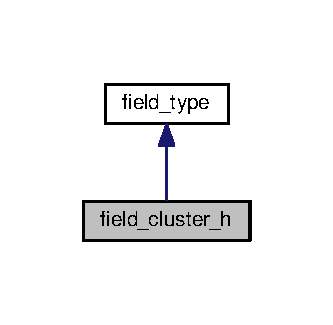
\includegraphics[width=160pt]{d0/d12/classfield__cluster__h__inherit__graph}
\end{center}
\end{figure}


Collaboration diagram for field\+\_\+cluster\+\_\+h\+:\nopagebreak
\begin{figure}[H]
\begin{center}
\leavevmode
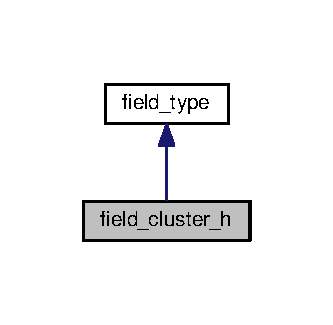
\includegraphics[width=160pt]{d3/dd8/classfield__cluster__h__coll__graph}
\end{center}
\end{figure}
\subsection*{Public Member Functions}
\begin{DoxyCompactItemize}
\item 
\hyperlink{classfield__cluster__h_a541bf81d40c5c5b6018c9d82f0eef578}{field\+\_\+cluster\+\_\+h} ()
\item 
\hyperlink{classfield__cluster__h_a8d0ea4d405ea4262a6681a25ffa74887}{field\+\_\+cluster\+\_\+h} (std\+::string filename)
\item 
\hyperlink{classfield__cluster__h_ab0eeee37bfb2f631c28e61c6e2086ad6}{field\+\_\+cluster\+\_\+h} (\hyperlink{classfield__type}{field\+\_\+type} \&other)
\item 
\hyperlink{classfield__cluster__h_a773569b54484ddff605306f368ea3641}{field\+\_\+cluster\+\_\+h} (const \hyperlink{classfield__cluster__h}{field\+\_\+cluster\+\_\+h} \&other)
\item 
\hyperlink{classfield__cluster__h_ad551ba1f8ee8cff03f97c6f5bdbd9133}{$\sim$field\+\_\+cluster\+\_\+h} ()
\item 
void \hyperlink{classfield__cluster__h_a5fd85ce8a88cb66118073e9b78ad42ba}{h\+\_\+access} (std\+::vector$<$ int $>$ \&position, std\+::vector$<$ double $>$ \&out)
\item 
void \hyperlink{classfield__cluster__h_a52bd59a7a1bd2be4c2aa83eedffe4a32}{h\+\_\+next} (bool \&finish, std\+::vector$<$ int $>$ \&pos, std\+::vector$<$ double $>$ \&out)
\item 
\hyperlink{classfield__cluster__h}{field\+\_\+cluster\+\_\+h} \& \hyperlink{classfield__cluster__h_aae54da56698bc8cf802d41fda39c0394}{operator=} (const \hyperlink{classfield__cluster__h}{field\+\_\+cluster\+\_\+h} \&other)
\item 
int \hyperlink{classfield__cluster__h_a8beeff6c5d5e7da194b5d57edcb04a08}{findnum} ()
\item 
void \hyperlink{classfield__cluster__h_a62630531cca5826f6077170d4f2fca94}{get\+\_\+1dfield\+\_\+h} (double $\ast$\&x, double $\ast$\&y, double $\ast$\&z) const 
\item 
void \hyperlink{classfield__cluster__h_a743d4b8bd643f1207ccf86d1e1a2f193}{fill\+\_\+rand} (std\+::vector$<$ int $>$ \&position)
\item 
bool \hyperlink{classfield__cluster__h_a0dd1c3a0c8b72ae2501dc5a06967b484}{check\+\_\+zero} (std\+::vector$<$ int $>$ \&position)
\item 
void \hyperlink{classfield__cluster__h_ad999087d163d4de0adc1e659703cf8a4}{change\+\_\+to\+\_\+test} (std\+::vector$<$ int $>$ \&position, \hyperlink{classham__type}{ham\+\_\+type} $\ast$hamil)
\end{DoxyCompactItemize}
\subsection*{Protected Attributes}
\begin{DoxyCompactItemize}
\item 
double $\ast$ \hyperlink{classfield__cluster__h_ace615b190c50eb2a398722b886ae2c9f}{spinx}
\item 
double $\ast$ \hyperlink{classfield__cluster__h_a1e9cb39e831864b2b0740fc4acb2106e}{spiny}
\item 
double $\ast$ \hyperlink{classfield__cluster__h_a11fa69cd080ca9d066fcf90f194ff3ef}{spinz}
\end{DoxyCompactItemize}


\subsection{Constructor \& Destructor Documentation}
\index{field\+\_\+cluster\+\_\+h@{field\+\_\+cluster\+\_\+h}!field\+\_\+cluster\+\_\+h@{field\+\_\+cluster\+\_\+h}}
\index{field\+\_\+cluster\+\_\+h@{field\+\_\+cluster\+\_\+h}!field\+\_\+cluster\+\_\+h@{field\+\_\+cluster\+\_\+h}}
\subsubsection[{\texorpdfstring{field\+\_\+cluster\+\_\+h()}{field_cluster_h()}}]{\setlength{\rightskip}{0pt plus 5cm}field\+\_\+cluster\+\_\+h\+::field\+\_\+cluster\+\_\+h (
\begin{DoxyParamCaption}
{}
\end{DoxyParamCaption}
)}\hypertarget{classfield__cluster__h_a541bf81d40c5c5b6018c9d82f0eef578}{}\label{classfield__cluster__h_a541bf81d40c5c5b6018c9d82f0eef578}
\index{field\+\_\+cluster\+\_\+h@{field\+\_\+cluster\+\_\+h}!field\+\_\+cluster\+\_\+h@{field\+\_\+cluster\+\_\+h}}
\index{field\+\_\+cluster\+\_\+h@{field\+\_\+cluster\+\_\+h}!field\+\_\+cluster\+\_\+h@{field\+\_\+cluster\+\_\+h}}
\subsubsection[{\texorpdfstring{field\+\_\+cluster\+\_\+h(std\+::string filename)}{field_cluster_h(std::string filename)}}]{\setlength{\rightskip}{0pt plus 5cm}field\+\_\+cluster\+\_\+h\+::field\+\_\+cluster\+\_\+h (
\begin{DoxyParamCaption}
\item[{std\+::string}]{filename}
\end{DoxyParamCaption}
)}\hypertarget{classfield__cluster__h_a8d0ea4d405ea4262a6681a25ffa74887}{}\label{classfield__cluster__h_a8d0ea4d405ea4262a6681a25ffa74887}
\index{field\+\_\+cluster\+\_\+h@{field\+\_\+cluster\+\_\+h}!field\+\_\+cluster\+\_\+h@{field\+\_\+cluster\+\_\+h}}
\index{field\+\_\+cluster\+\_\+h@{field\+\_\+cluster\+\_\+h}!field\+\_\+cluster\+\_\+h@{field\+\_\+cluster\+\_\+h}}
\subsubsection[{\texorpdfstring{field\+\_\+cluster\+\_\+h(field\+\_\+type \&other)}{field_cluster_h(field_type &other)}}]{\setlength{\rightskip}{0pt plus 5cm}field\+\_\+cluster\+\_\+h\+::field\+\_\+cluster\+\_\+h (
\begin{DoxyParamCaption}
\item[{{\bf field\+\_\+type} \&}]{other}
\end{DoxyParamCaption}
)}\hypertarget{classfield__cluster__h_ab0eeee37bfb2f631c28e61c6e2086ad6}{}\label{classfield__cluster__h_ab0eeee37bfb2f631c28e61c6e2086ad6}
\index{field\+\_\+cluster\+\_\+h@{field\+\_\+cluster\+\_\+h}!field\+\_\+cluster\+\_\+h@{field\+\_\+cluster\+\_\+h}}
\index{field\+\_\+cluster\+\_\+h@{field\+\_\+cluster\+\_\+h}!field\+\_\+cluster\+\_\+h@{field\+\_\+cluster\+\_\+h}}
\subsubsection[{\texorpdfstring{field\+\_\+cluster\+\_\+h(const field\+\_\+cluster\+\_\+h \&other)}{field_cluster_h(const field_cluster_h &other)}}]{\setlength{\rightskip}{0pt plus 5cm}field\+\_\+cluster\+\_\+h\+::field\+\_\+cluster\+\_\+h (
\begin{DoxyParamCaption}
\item[{const {\bf field\+\_\+cluster\+\_\+h} \&}]{other}
\end{DoxyParamCaption}
)}\hypertarget{classfield__cluster__h_a773569b54484ddff605306f368ea3641}{}\label{classfield__cluster__h_a773569b54484ddff605306f368ea3641}
\index{field\+\_\+cluster\+\_\+h@{field\+\_\+cluster\+\_\+h}!````~field\+\_\+cluster\+\_\+h@{$\sim$field\+\_\+cluster\+\_\+h}}
\index{````~field\+\_\+cluster\+\_\+h@{$\sim$field\+\_\+cluster\+\_\+h}!field\+\_\+cluster\+\_\+h@{field\+\_\+cluster\+\_\+h}}
\subsubsection[{\texorpdfstring{$\sim$field\+\_\+cluster\+\_\+h()}{~field_cluster_h()}}]{\setlength{\rightskip}{0pt plus 5cm}field\+\_\+cluster\+\_\+h\+::$\sim$field\+\_\+cluster\+\_\+h (
\begin{DoxyParamCaption}
{}
\end{DoxyParamCaption}
)}\hypertarget{classfield__cluster__h_ad551ba1f8ee8cff03f97c6f5bdbd9133}{}\label{classfield__cluster__h_ad551ba1f8ee8cff03f97c6f5bdbd9133}


\subsection{Member Function Documentation}
\index{field\+\_\+cluster\+\_\+h@{field\+\_\+cluster\+\_\+h}!change\+\_\+to\+\_\+test@{change\+\_\+to\+\_\+test}}
\index{change\+\_\+to\+\_\+test@{change\+\_\+to\+\_\+test}!field\+\_\+cluster\+\_\+h@{field\+\_\+cluster\+\_\+h}}
\subsubsection[{\texorpdfstring{change\+\_\+to\+\_\+test(std\+::vector$<$ int $>$ \&position, ham\+\_\+type $\ast$hamil)}{change_to_test(std::vector< int > &position, ham_type *hamil)}}]{\setlength{\rightskip}{0pt plus 5cm}void field\+\_\+cluster\+\_\+h\+::change\+\_\+to\+\_\+test (
\begin{DoxyParamCaption}
\item[{std\+::vector$<$ int $>$ \&}]{position, }
\item[{{\bf ham\+\_\+type} $\ast$}]{hamil}
\end{DoxyParamCaption}
)\hspace{0.3cm}{\ttfamily [virtual]}}\hypertarget{classfield__cluster__h_ad999087d163d4de0adc1e659703cf8a4}{}\label{classfield__cluster__h_ad999087d163d4de0adc1e659703cf8a4}


Reimplemented from \hyperlink{classfield__type_a32140b8a785c0139dd27304143ca5f17}{field\+\_\+type}.

\index{field\+\_\+cluster\+\_\+h@{field\+\_\+cluster\+\_\+h}!check\+\_\+zero@{check\+\_\+zero}}
\index{check\+\_\+zero@{check\+\_\+zero}!field\+\_\+cluster\+\_\+h@{field\+\_\+cluster\+\_\+h}}
\subsubsection[{\texorpdfstring{check\+\_\+zero(std\+::vector$<$ int $>$ \&position)}{check_zero(std::vector< int > &position)}}]{\setlength{\rightskip}{0pt plus 5cm}bool field\+\_\+cluster\+\_\+h\+::check\+\_\+zero (
\begin{DoxyParamCaption}
\item[{std\+::vector$<$ int $>$ \&}]{position}
\end{DoxyParamCaption}
)\hspace{0.3cm}{\ttfamily [inline]}, {\ttfamily [virtual]}}\hypertarget{classfield__cluster__h_a0dd1c3a0c8b72ae2501dc5a06967b484}{}\label{classfield__cluster__h_a0dd1c3a0c8b72ae2501dc5a06967b484}


Reimplemented from \hyperlink{classfield__type_a8aabf0f54a8dc73b1ac529a26604c827}{field\+\_\+type}.

\index{field\+\_\+cluster\+\_\+h@{field\+\_\+cluster\+\_\+h}!fill\+\_\+rand@{fill\+\_\+rand}}
\index{fill\+\_\+rand@{fill\+\_\+rand}!field\+\_\+cluster\+\_\+h@{field\+\_\+cluster\+\_\+h}}
\subsubsection[{\texorpdfstring{fill\+\_\+rand(std\+::vector$<$ int $>$ \&position)}{fill_rand(std::vector< int > &position)}}]{\setlength{\rightskip}{0pt plus 5cm}void field\+\_\+cluster\+\_\+h\+::fill\+\_\+rand (
\begin{DoxyParamCaption}
\item[{std\+::vector$<$ int $>$ \&}]{position}
\end{DoxyParamCaption}
)\hspace{0.3cm}{\ttfamily [inline]}, {\ttfamily [virtual]}}\hypertarget{classfield__cluster__h_a743d4b8bd643f1207ccf86d1e1a2f193}{}\label{classfield__cluster__h_a743d4b8bd643f1207ccf86d1e1a2f193}


Reimplemented from \hyperlink{classfield__type_a87d6bf8e9e97ce158a356fefaddc3bee}{field\+\_\+type}.

\index{field\+\_\+cluster\+\_\+h@{field\+\_\+cluster\+\_\+h}!findnum@{findnum}}
\index{findnum@{findnum}!field\+\_\+cluster\+\_\+h@{field\+\_\+cluster\+\_\+h}}
\subsubsection[{\texorpdfstring{findnum()}{findnum()}}]{\setlength{\rightskip}{0pt plus 5cm}int field\+\_\+cluster\+\_\+h\+::findnum (
\begin{DoxyParamCaption}
{}
\end{DoxyParamCaption}
)\hspace{0.3cm}{\ttfamily [inline]}, {\ttfamily [virtual]}}\hypertarget{classfield__cluster__h_a8beeff6c5d5e7da194b5d57edcb04a08}{}\label{classfield__cluster__h_a8beeff6c5d5e7da194b5d57edcb04a08}


Reimplemented from \hyperlink{classfield__type_a73e5605cfd2714b2a358d61c4b102883}{field\+\_\+type}.

\index{field\+\_\+cluster\+\_\+h@{field\+\_\+cluster\+\_\+h}!get\+\_\+1dfield\+\_\+h@{get\+\_\+1dfield\+\_\+h}}
\index{get\+\_\+1dfield\+\_\+h@{get\+\_\+1dfield\+\_\+h}!field\+\_\+cluster\+\_\+h@{field\+\_\+cluster\+\_\+h}}
\subsubsection[{\texorpdfstring{get\+\_\+1dfield\+\_\+h(double $\ast$\&x, double $\ast$\&y, double $\ast$\&z) const }{get_1dfield_h(double *&x, double *&y, double *&z) const }}]{\setlength{\rightskip}{0pt plus 5cm}void field\+\_\+cluster\+\_\+h\+::get\+\_\+1dfield\+\_\+h (
\begin{DoxyParamCaption}
\item[{double $\ast$\&}]{x, }
\item[{double $\ast$\&}]{y, }
\item[{double $\ast$\&}]{z}
\end{DoxyParamCaption}
) const\hspace{0.3cm}{\ttfamily [virtual]}}\hypertarget{classfield__cluster__h_a62630531cca5826f6077170d4f2fca94}{}\label{classfield__cluster__h_a62630531cca5826f6077170d4f2fca94}


Reimplemented from \hyperlink{classfield__type_aa3c7c5992e51d5588601e1a8681c6ae1}{field\+\_\+type}.

\index{field\+\_\+cluster\+\_\+h@{field\+\_\+cluster\+\_\+h}!h\+\_\+access@{h\+\_\+access}}
\index{h\+\_\+access@{h\+\_\+access}!field\+\_\+cluster\+\_\+h@{field\+\_\+cluster\+\_\+h}}
\subsubsection[{\texorpdfstring{h\+\_\+access(std\+::vector$<$ int $>$ \&position, std\+::vector$<$ double $>$ \&out)}{h_access(std::vector< int > &position, std::vector< double > &out)}}]{\setlength{\rightskip}{0pt plus 5cm}void field\+\_\+cluster\+\_\+h\+::h\+\_\+access (
\begin{DoxyParamCaption}
\item[{std\+::vector$<$ int $>$ \&}]{position, }
\item[{std\+::vector$<$ double $>$ \&}]{out}
\end{DoxyParamCaption}
)\hspace{0.3cm}{\ttfamily [virtual]}}\hypertarget{classfield__cluster__h_a5fd85ce8a88cb66118073e9b78ad42ba}{}\label{classfield__cluster__h_a5fd85ce8a88cb66118073e9b78ad42ba}


Reimplemented from \hyperlink{classfield__type_ada65523f1a000cbd929f2d97d747fa59}{field\+\_\+type}.

\index{field\+\_\+cluster\+\_\+h@{field\+\_\+cluster\+\_\+h}!h\+\_\+next@{h\+\_\+next}}
\index{h\+\_\+next@{h\+\_\+next}!field\+\_\+cluster\+\_\+h@{field\+\_\+cluster\+\_\+h}}
\subsubsection[{\texorpdfstring{h\+\_\+next(bool \&finish, std\+::vector$<$ int $>$ \&pos, std\+::vector$<$ double $>$ \&out)}{h_next(bool &finish, std::vector< int > &pos, std::vector< double > &out)}}]{\setlength{\rightskip}{0pt plus 5cm}void field\+\_\+cluster\+\_\+h\+::h\+\_\+next (
\begin{DoxyParamCaption}
\item[{bool \&}]{finish, }
\item[{std\+::vector$<$ int $>$ \&}]{pos, }
\item[{std\+::vector$<$ double $>$ \&}]{out}
\end{DoxyParamCaption}
)\hspace{0.3cm}{\ttfamily [virtual]}}\hypertarget{classfield__cluster__h_a52bd59a7a1bd2be4c2aa83eedffe4a32}{}\label{classfield__cluster__h_a52bd59a7a1bd2be4c2aa83eedffe4a32}


Reimplemented from \hyperlink{classfield__type_a4f68c166bbd86806584f44c6d6faf50f}{field\+\_\+type}.

\index{field\+\_\+cluster\+\_\+h@{field\+\_\+cluster\+\_\+h}!operator=@{operator=}}
\index{operator=@{operator=}!field\+\_\+cluster\+\_\+h@{field\+\_\+cluster\+\_\+h}}
\subsubsection[{\texorpdfstring{operator=(const field\+\_\+cluster\+\_\+h \&other)}{operator=(const field_cluster_h &other)}}]{\setlength{\rightskip}{0pt plus 5cm}{\bf field\+\_\+cluster\+\_\+h}\& field\+\_\+cluster\+\_\+h\+::operator= (
\begin{DoxyParamCaption}
\item[{const {\bf field\+\_\+cluster\+\_\+h} \&}]{other}
\end{DoxyParamCaption}
)}\hypertarget{classfield__cluster__h_aae54da56698bc8cf802d41fda39c0394}{}\label{classfield__cluster__h_aae54da56698bc8cf802d41fda39c0394}


\subsection{Member Data Documentation}
\index{field\+\_\+cluster\+\_\+h@{field\+\_\+cluster\+\_\+h}!spinx@{spinx}}
\index{spinx@{spinx}!field\+\_\+cluster\+\_\+h@{field\+\_\+cluster\+\_\+h}}
\subsubsection[{\texorpdfstring{spinx}{spinx}}]{\setlength{\rightskip}{0pt plus 5cm}double$\ast$ field\+\_\+cluster\+\_\+h\+::spinx\hspace{0.3cm}{\ttfamily [protected]}}\hypertarget{classfield__cluster__h_ace615b190c50eb2a398722b886ae2c9f}{}\label{classfield__cluster__h_ace615b190c50eb2a398722b886ae2c9f}
\index{field\+\_\+cluster\+\_\+h@{field\+\_\+cluster\+\_\+h}!spiny@{spiny}}
\index{spiny@{spiny}!field\+\_\+cluster\+\_\+h@{field\+\_\+cluster\+\_\+h}}
\subsubsection[{\texorpdfstring{spiny}{spiny}}]{\setlength{\rightskip}{0pt plus 5cm}double$\ast$ field\+\_\+cluster\+\_\+h\+::spiny\hspace{0.3cm}{\ttfamily [protected]}}\hypertarget{classfield__cluster__h_a1e9cb39e831864b2b0740fc4acb2106e}{}\label{classfield__cluster__h_a1e9cb39e831864b2b0740fc4acb2106e}
\index{field\+\_\+cluster\+\_\+h@{field\+\_\+cluster\+\_\+h}!spinz@{spinz}}
\index{spinz@{spinz}!field\+\_\+cluster\+\_\+h@{field\+\_\+cluster\+\_\+h}}
\subsubsection[{\texorpdfstring{spinz}{spinz}}]{\setlength{\rightskip}{0pt plus 5cm}double$\ast$ field\+\_\+cluster\+\_\+h\+::spinz\hspace{0.3cm}{\ttfamily [protected]}}\hypertarget{classfield__cluster__h_a11fa69cd080ca9d066fcf90f194ff3ef}{}\label{classfield__cluster__h_a11fa69cd080ca9d066fcf90f194ff3ef}


The documentation for this class was generated from the following file\+:\begin{DoxyCompactItemize}
\item 
includes/\hyperlink{field__type_8hpp}{field\+\_\+type.\+hpp}\end{DoxyCompactItemize}

\hypertarget{classfield__type}{}\section{field\+\_\+type Class Reference}
\label{classfield__type}\index{field\+\_\+type@{field\+\_\+type}}


{\ttfamily \#include $<$field\+\_\+type.\+hpp$>$}



Inheritance diagram for field\+\_\+type\+:\nopagebreak
\begin{figure}[H]
\begin{center}
\leavevmode
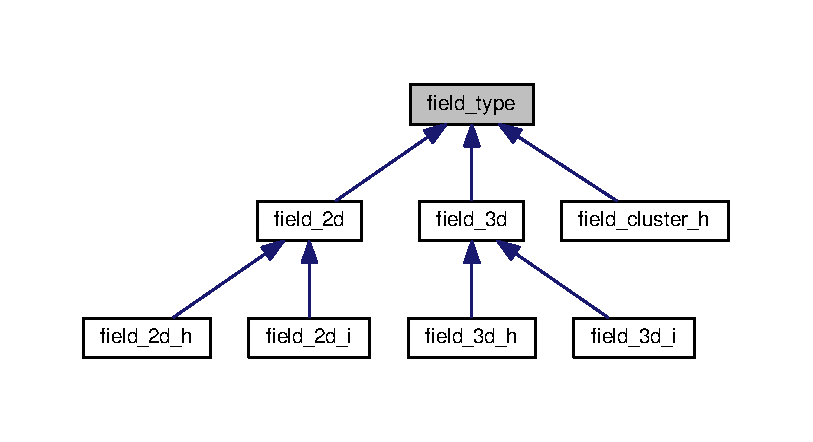
\includegraphics[width=350pt]{de/da8/classfield__type__inherit__graph}
\end{center}
\end{figure}
\subsection*{Public Member Functions}
\begin{DoxyCompactItemize}
\item 
\hyperlink{classfield__type_a57c28e2caacf2ff4422ea1206cf0efae}{field\+\_\+type} ()
\item 
\hyperlink{classfield__type_aabdd13b4a98dcabc63b75867c80ceae3}{$\sim$field\+\_\+type} ()
\item 
virtual void \hyperlink{classfield__type_a0941f94d7f73234d02c69faf2a0f6e5e}{i\+\_\+access} (std\+::vector$<$ int $>$ \&postion, int \&out)
\item 
virtual void \hyperlink{classfield__type_aaaea375b4de0d0ef9ca4427832611584}{i\+\_\+adjacent} (std\+::vector$<$ int $>$ \&position, int $\ast$out)
\item 
virtual void \hyperlink{classfield__type_ada65523f1a000cbd929f2d97d747fa59}{h\+\_\+access} (std\+::vector$<$ int $>$ \&position, std\+::vector$<$ double $>$ \&out)
\item 
virtual void \hyperlink{classfield__type_af91a0a4b7d3076c41baa96f25faec0c4}{h\+\_\+adjacent} (std\+::vector$<$ int $>$ \&position, double $\ast$$\ast$out)
\item 
virtual void \hyperlink{classfield__type_a77964e0d6f8d20c9a1ec579847570c4c}{h\+\_\+2adjacent} (std\+::vector$<$ int $>$ \&position, double $\ast$$\ast$out)
\item 
virtual void \hyperlink{classfield__type_a293169a5ca7f03b818c0aa92410a5078}{h\+\_\+arb\+\_\+adj} (std\+::vector$<$ int $>$ \&position, std\+::vector$<$ int $>$ \&dxs, std\+::vector$<$ int $>$ \&dys, std\+::vector$<$ int $>$ \&dzs, double $\ast$$\ast$out, int num)
\item 
virtual void \hyperlink{classfield__type_afaf4b3449a0ee906ebe543439054eab5}{next} (bool \&finish, std\+::vector$<$ int $>$ \&pos)
\item 
virtual void \hyperlink{classfield__type_a0785839e047ace8841ded448d49900ca}{i\+\_\+next} (bool \&finish, std\+::vector$<$ int $>$ \&pos, int \&out)
\item 
virtual void \hyperlink{classfield__type_a4f68c166bbd86806584f44c6d6faf50f}{h\+\_\+next} (bool \&finish, std\+::vector$<$ int $>$ \&pos, std\+::vector$<$ double $>$ \&out)
\item 
int \hyperlink{classfield__type_a3049cba266e811fcd2bc85795bf90bab}{get\+\_\+insize} () const 
\item 
int \hyperlink{classfield__type_a755a2d8e406f7b1839f9b9fa095cce4d}{get\+\_\+totsize} () const 
\item 
bool \hyperlink{classfield__type_a9f7358804d7ea934d4f0f896cd48217b}{get\+\_\+perio} () const 
\item 
int \hyperlink{classfield__type_a6645c4ee6bab91e9d75986b5d8d385dd}{get\+\_\+dim} () const 
\item 
virtual void \hyperlink{classfield__type_a11c23271c828983406e8e80c66b81c46}{fill\+\_\+ghost} (int num\+\_\+rows)
\item 
virtual void \hyperlink{classfield__type_a87d6bf8e9e97ce158a356fefaddc3bee}{fill\+\_\+rand} (std\+::vector$<$ int $>$ \&position)
\item 
virtual void \hyperlink{classfield__type_afdb5b29e839fa11c7faeff60ee49aebb}{fill\+\_\+zero} (std\+::vector$<$ int $>$ \&position)
\item 
virtual void \hyperlink{classfield__type_acb4fb5c3393feed8685eb3957c032a15}{fill\+\_\+one} (std\+::vector$<$ int $>$ \&position)
\item 
virtual void \hyperlink{classfield__type_a0d6034d05532edaa10fbc0f102180b9d}{fill\+\_\+val\+\_\+i} (std\+::vector$<$ int $>$ \&position, int val)
\item 
virtual void \hyperlink{classfield__type_a02500bfb9021cf13ff6e1be66b63b9ae}{fill\+\_\+val\+\_\+h} (std\+::vector$<$ int $>$ \&position, double x, double y, double z)
\item 
virtual void \hyperlink{classfield__type_a35a20297e1cddac40d4c2aecef5a5594}{add\+\_\+val\+\_\+h} (std\+::vector$<$ int $>$ \&position, std\+::vector$<$ double $>$ \&in)
\item 
void \hyperlink{classfield__type_aba179be6c700a5aeaa5507dbed35a977}{allzero} ()
\item 
virtual bool \hyperlink{classfield__type_a8aabf0f54a8dc73b1ac529a26604c827}{check\+\_\+zero} (std\+::vector$<$ int $>$ \&position)
\item 
virtual void \hyperlink{classfield__type_a32140b8a785c0139dd27304143ca5f17}{change\+\_\+to\+\_\+test} (std\+::vector$<$ int $>$ \&position, \hyperlink{classham__type}{ham\+\_\+type} $\ast$hamil)
\item 
virtual void \hyperlink{classfield__type_a4677e4a96fded67b1f494b7716092d90}{new\+\_\+mem} ()
\item 
virtual int \hyperlink{classfield__type_a73e5605cfd2714b2a358d61c4b102883}{findnum} ()
\item 
virtual void \hyperlink{classfield__type_a1227fb5db27d6a4f2de5662c0aecde53}{get\+\_\+2dfield\+\_\+i} (int $\ast$$\ast$\&x) const 
\item 
virtual void \hyperlink{classfield__type_ac005ee44a3ffc5feabda864e181f8c28}{get\+\_\+3dfield\+\_\+i} (int $\ast$$\ast$$\ast$\&x) const 
\item 
virtual void \hyperlink{classfield__type_aa3c7c5992e51d5588601e1a8681c6ae1}{get\+\_\+1dfield\+\_\+h} (double $\ast$\&x, double $\ast$\&y, double $\ast$\&z) const 
\item 
virtual void \hyperlink{classfield__type_af15dfa4de69c756148f82628b095b22e}{get\+\_\+2dfield\+\_\+h} (double $\ast$$\ast$\&x, double $\ast$$\ast$\&y, double $\ast$$\ast$\&z) const 
\item 
virtual void \hyperlink{classfield__type_ae8649f8841a9c363914d4f72cea4df5f}{get\+\_\+3dfield\+\_\+h} (double $\ast$$\ast$$\ast$\&x, double $\ast$$\ast$$\ast$\&y, double $\ast$$\ast$$\ast$\&z) const 
\item 
virtual void \hyperlink{classfield__type_a4924396b413bb7f5a43e6602561bdfbf}{get\+\_\+2dzero} (bool $\ast$$\ast$\&x) const 
\item 
virtual void \hyperlink{classfield__type_aa6fa2f915583fc2941db7713138d8f8b}{get\+\_\+3dzero} (bool $\ast$$\ast$$\ast$\&x) const 
\item 
virtual void \hyperlink{classfield__type_a70fd2b76f1a1bf1604bcdb39d99687d2}{print} (std\+::string filename, std\+::string arrname)
\item 
virtual void \hyperlink{classfield__type_a1429809586fadd4afa829bef77fa819d}{print\+\_\+setup} (const std\+::string filename, const std\+::string groupname, const int Tmax, const int Hmax)
\item 
int \hyperlink{classfield__type_a66e2771b5ddf65d5f7c4e5bcb3186d2f}{get\+\_\+ft} () const 
\item 
virtual void \hyperlink{classfield__type_afaabc410e2ce254c23e3c4aa39d1916d}{send\+\_\+data} (int dest\+\_\+rank)
\item 
virtual void \hyperlink{classfield__type_ac29bf02760384b80a08e5e57ca43542f}{recv\+\_\+data} (int src\+\_\+rank)
\end{DoxyCompactItemize}
\subsection*{Protected Attributes}
\begin{DoxyCompactItemize}
\item 
int \hyperlink{classfield__type_a6122e0fff3bcc40a158369cd3fd19c88}{ft}
\item 
int \hyperlink{classfield__type_a58b576356c02b88ea686aa9937e527f6}{dim}
\item 
int \hyperlink{classfield__type_adcbc745f653a086ececd263baddde7f1}{insize}
\item 
int \hyperlink{classfield__type_ad74b0d86e6384925090cdf090f1e90f5}{totsize}
\item 
bool \hyperlink{classfield__type_a44d8b06e823939f2dda6706cb38a3280}{periodic}
\end{DoxyCompactItemize}


\subsection{Constructor \& Destructor Documentation}
\index{field\+\_\+type@{field\+\_\+type}!field\+\_\+type@{field\+\_\+type}}
\index{field\+\_\+type@{field\+\_\+type}!field\+\_\+type@{field\+\_\+type}}
\subsubsection[{\texorpdfstring{field\+\_\+type()}{field_type()}}]{\setlength{\rightskip}{0pt plus 5cm}field\+\_\+type\+::field\+\_\+type (
\begin{DoxyParamCaption}
{}
\end{DoxyParamCaption}
)\hspace{0.3cm}{\ttfamily [inline]}}\hypertarget{classfield__type_a57c28e2caacf2ff4422ea1206cf0efae}{}\label{classfield__type_a57c28e2caacf2ff4422ea1206cf0efae}
\index{field\+\_\+type@{field\+\_\+type}!````~field\+\_\+type@{$\sim$field\+\_\+type}}
\index{````~field\+\_\+type@{$\sim$field\+\_\+type}!field\+\_\+type@{field\+\_\+type}}
\subsubsection[{\texorpdfstring{$\sim$field\+\_\+type()}{~field_type()}}]{\setlength{\rightskip}{0pt plus 5cm}field\+\_\+type\+::$\sim$field\+\_\+type (
\begin{DoxyParamCaption}
{}
\end{DoxyParamCaption}
)\hspace{0.3cm}{\ttfamily [inline]}}\hypertarget{classfield__type_aabdd13b4a98dcabc63b75867c80ceae3}{}\label{classfield__type_aabdd13b4a98dcabc63b75867c80ceae3}


\subsection{Member Function Documentation}
\index{field\+\_\+type@{field\+\_\+type}!add\+\_\+val\+\_\+h@{add\+\_\+val\+\_\+h}}
\index{add\+\_\+val\+\_\+h@{add\+\_\+val\+\_\+h}!field\+\_\+type@{field\+\_\+type}}
\subsubsection[{\texorpdfstring{add\+\_\+val\+\_\+h(std\+::vector$<$ int $>$ \&position, std\+::vector$<$ double $>$ \&in)}{add_val_h(std::vector< int > &position, std::vector< double > &in)}}]{\setlength{\rightskip}{0pt plus 5cm}virtual void field\+\_\+type\+::add\+\_\+val\+\_\+h (
\begin{DoxyParamCaption}
\item[{std\+::vector$<$ int $>$ \&}]{position, }
\item[{std\+::vector$<$ double $>$ \&}]{in}
\end{DoxyParamCaption}
)\hspace{0.3cm}{\ttfamily [inline]}, {\ttfamily [virtual]}}\hypertarget{classfield__type_a35a20297e1cddac40d4c2aecef5a5594}{}\label{classfield__type_a35a20297e1cddac40d4c2aecef5a5594}


Reimplemented in \hyperlink{classfield__3d__h_a90b81a79c986e2b8ec3243a75eec7663}{field\+\_\+3d\+\_\+h}, and \hyperlink{classfield__2d__h_aa8777664592ab4317bca3734497e2404}{field\+\_\+2d\+\_\+h}.

\index{field\+\_\+type@{field\+\_\+type}!allzero@{allzero}}
\index{allzero@{allzero}!field\+\_\+type@{field\+\_\+type}}
\subsubsection[{\texorpdfstring{allzero()}{allzero()}}]{\setlength{\rightskip}{0pt plus 5cm}void field\+\_\+type\+::allzero (
\begin{DoxyParamCaption}
{}
\end{DoxyParamCaption}
)}\hypertarget{classfield__type_aba179be6c700a5aeaa5507dbed35a977}{}\label{classfield__type_aba179be6c700a5aeaa5507dbed35a977}
\index{field\+\_\+type@{field\+\_\+type}!change\+\_\+to\+\_\+test@{change\+\_\+to\+\_\+test}}
\index{change\+\_\+to\+\_\+test@{change\+\_\+to\+\_\+test}!field\+\_\+type@{field\+\_\+type}}
\subsubsection[{\texorpdfstring{change\+\_\+to\+\_\+test(std\+::vector$<$ int $>$ \&position, ham\+\_\+type $\ast$hamil)}{change_to_test(std::vector< int > &position, ham_type *hamil)}}]{\setlength{\rightskip}{0pt plus 5cm}virtual void field\+\_\+type\+::change\+\_\+to\+\_\+test (
\begin{DoxyParamCaption}
\item[{std\+::vector$<$ int $>$ \&}]{position, }
\item[{{\bf ham\+\_\+type} $\ast$}]{hamil}
\end{DoxyParamCaption}
)\hspace{0.3cm}{\ttfamily [inline]}, {\ttfamily [virtual]}}\hypertarget{classfield__type_a32140b8a785c0139dd27304143ca5f17}{}\label{classfield__type_a32140b8a785c0139dd27304143ca5f17}


Reimplemented in \hyperlink{classfield__3d__i_a4f027dbc1d8b205fff6e967c9748f0c6}{field\+\_\+3d\+\_\+i}, \hyperlink{classfield__3d__h_a5bd770e759efdc768af894b3a57a8b90}{field\+\_\+3d\+\_\+h}, \hyperlink{classfield__2d__i_a67325e8fc578af047dd367aa3d679b25}{field\+\_\+2d\+\_\+i}, \hyperlink{classfield__2d__h_a87173eff35d950aeb70b0c955c5c0e5d}{field\+\_\+2d\+\_\+h}, and \hyperlink{classfield__cluster__h_ad999087d163d4de0adc1e659703cf8a4}{field\+\_\+cluster\+\_\+h}.

\index{field\+\_\+type@{field\+\_\+type}!check\+\_\+zero@{check\+\_\+zero}}
\index{check\+\_\+zero@{check\+\_\+zero}!field\+\_\+type@{field\+\_\+type}}
\subsubsection[{\texorpdfstring{check\+\_\+zero(std\+::vector$<$ int $>$ \&position)}{check_zero(std::vector< int > &position)}}]{\setlength{\rightskip}{0pt plus 5cm}virtual bool field\+\_\+type\+::check\+\_\+zero (
\begin{DoxyParamCaption}
\item[{std\+::vector$<$ int $>$ \&}]{position}
\end{DoxyParamCaption}
)\hspace{0.3cm}{\ttfamily [inline]}, {\ttfamily [virtual]}}\hypertarget{classfield__type_a8aabf0f54a8dc73b1ac529a26604c827}{}\label{classfield__type_a8aabf0f54a8dc73b1ac529a26604c827}


Reimplemented in \hyperlink{classfield__3d_a18debdb40fa4de1d676cc64f0c4a9c85}{field\+\_\+3d}, \hyperlink{classfield__2d_a72e41b87dc96e59d6bc636cc1a4ca44d}{field\+\_\+2d}, and \hyperlink{classfield__cluster__h_a0dd1c3a0c8b72ae2501dc5a06967b484}{field\+\_\+cluster\+\_\+h}.

\index{field\+\_\+type@{field\+\_\+type}!fill\+\_\+ghost@{fill\+\_\+ghost}}
\index{fill\+\_\+ghost@{fill\+\_\+ghost}!field\+\_\+type@{field\+\_\+type}}
\subsubsection[{\texorpdfstring{fill\+\_\+ghost(int num\+\_\+rows)}{fill_ghost(int num_rows)}}]{\setlength{\rightskip}{0pt plus 5cm}virtual void field\+\_\+type\+::fill\+\_\+ghost (
\begin{DoxyParamCaption}
\item[{int}]{num\+\_\+rows}
\end{DoxyParamCaption}
)\hspace{0.3cm}{\ttfamily [inline]}, {\ttfamily [virtual]}}\hypertarget{classfield__type_a11c23271c828983406e8e80c66b81c46}{}\label{classfield__type_a11c23271c828983406e8e80c66b81c46}


Reimplemented in \hyperlink{classfield__3d__i_a5c7a0ce8daedd401bdd8c6c57bd5343c}{field\+\_\+3d\+\_\+i}, \hyperlink{classfield__3d__h_a1591db771816e1dd5b9971463cd14988}{field\+\_\+3d\+\_\+h}, \hyperlink{classfield__2d__i_aa4d7c1c2e6fb75459b0cc009f29293f1}{field\+\_\+2d\+\_\+i}, and \hyperlink{classfield__2d__h_a94fe388174d778328629ad3fb4c13566}{field\+\_\+2d\+\_\+h}.

\index{field\+\_\+type@{field\+\_\+type}!fill\+\_\+one@{fill\+\_\+one}}
\index{fill\+\_\+one@{fill\+\_\+one}!field\+\_\+type@{field\+\_\+type}}
\subsubsection[{\texorpdfstring{fill\+\_\+one(std\+::vector$<$ int $>$ \&position)}{fill_one(std::vector< int > &position)}}]{\setlength{\rightskip}{0pt plus 5cm}virtual void field\+\_\+type\+::fill\+\_\+one (
\begin{DoxyParamCaption}
\item[{std\+::vector$<$ int $>$ \&}]{position}
\end{DoxyParamCaption}
)\hspace{0.3cm}{\ttfamily [inline]}, {\ttfamily [virtual]}}\hypertarget{classfield__type_acb4fb5c3393feed8685eb3957c032a15}{}\label{classfield__type_acb4fb5c3393feed8685eb3957c032a15}


Reimplemented in \hyperlink{classfield__3d__i_a3500aa4597707f620d1c2f4a51936faa}{field\+\_\+3d\+\_\+i}, \hyperlink{classfield__3d__h_aa703c9cc42ed4f072e0defce344d4de3}{field\+\_\+3d\+\_\+h}, \hyperlink{classfield__2d__i_a859791e738fa2340ac579f4466a67a2f}{field\+\_\+2d\+\_\+i}, and \hyperlink{classfield__2d__h_ac4ef3e08335182c46bfb6ff37cf447cd}{field\+\_\+2d\+\_\+h}.

\index{field\+\_\+type@{field\+\_\+type}!fill\+\_\+rand@{fill\+\_\+rand}}
\index{fill\+\_\+rand@{fill\+\_\+rand}!field\+\_\+type@{field\+\_\+type}}
\subsubsection[{\texorpdfstring{fill\+\_\+rand(std\+::vector$<$ int $>$ \&position)}{fill_rand(std::vector< int > &position)}}]{\setlength{\rightskip}{0pt plus 5cm}virtual void field\+\_\+type\+::fill\+\_\+rand (
\begin{DoxyParamCaption}
\item[{std\+::vector$<$ int $>$ \&}]{position}
\end{DoxyParamCaption}
)\hspace{0.3cm}{\ttfamily [inline]}, {\ttfamily [virtual]}}\hypertarget{classfield__type_a87d6bf8e9e97ce158a356fefaddc3bee}{}\label{classfield__type_a87d6bf8e9e97ce158a356fefaddc3bee}


Reimplemented in \hyperlink{classfield__3d__i_a014cb8a3b6feb90c7af771960b53fda7}{field\+\_\+3d\+\_\+i}, \hyperlink{classfield__3d__h_a85ce1558d9260abb50dbbf0a210764ba}{field\+\_\+3d\+\_\+h}, \hyperlink{classfield__2d__i_ad0c4a3a9efde2bb4abfb131b3acfb7c2}{field\+\_\+2d\+\_\+i}, \hyperlink{classfield__2d__h_a3a4c57fdf1ce84f4e6006bb37a76ec58}{field\+\_\+2d\+\_\+h}, and \hyperlink{classfield__cluster__h_a743d4b8bd643f1207ccf86d1e1a2f193}{field\+\_\+cluster\+\_\+h}.

\index{field\+\_\+type@{field\+\_\+type}!fill\+\_\+val\+\_\+h@{fill\+\_\+val\+\_\+h}}
\index{fill\+\_\+val\+\_\+h@{fill\+\_\+val\+\_\+h}!field\+\_\+type@{field\+\_\+type}}
\subsubsection[{\texorpdfstring{fill\+\_\+val\+\_\+h(std\+::vector$<$ int $>$ \&position, double x, double y, double z)}{fill_val_h(std::vector< int > &position, double x, double y, double z)}}]{\setlength{\rightskip}{0pt plus 5cm}virtual void field\+\_\+type\+::fill\+\_\+val\+\_\+h (
\begin{DoxyParamCaption}
\item[{std\+::vector$<$ int $>$ \&}]{position, }
\item[{double}]{x, }
\item[{double}]{y, }
\item[{double}]{z}
\end{DoxyParamCaption}
)\hspace{0.3cm}{\ttfamily [inline]}, {\ttfamily [virtual]}}\hypertarget{classfield__type_a02500bfb9021cf13ff6e1be66b63b9ae}{}\label{classfield__type_a02500bfb9021cf13ff6e1be66b63b9ae}


Reimplemented in \hyperlink{classfield__3d__h_a11e90275cade149683013d09e9dd9756}{field\+\_\+3d\+\_\+h}, and \hyperlink{classfield__2d__h_a9a0a35285e1a3995e2768a8b43c4855a}{field\+\_\+2d\+\_\+h}.

\index{field\+\_\+type@{field\+\_\+type}!fill\+\_\+val\+\_\+i@{fill\+\_\+val\+\_\+i}}
\index{fill\+\_\+val\+\_\+i@{fill\+\_\+val\+\_\+i}!field\+\_\+type@{field\+\_\+type}}
\subsubsection[{\texorpdfstring{fill\+\_\+val\+\_\+i(std\+::vector$<$ int $>$ \&position, int val)}{fill_val_i(std::vector< int > &position, int val)}}]{\setlength{\rightskip}{0pt plus 5cm}virtual void field\+\_\+type\+::fill\+\_\+val\+\_\+i (
\begin{DoxyParamCaption}
\item[{std\+::vector$<$ int $>$ \&}]{position, }
\item[{int}]{val}
\end{DoxyParamCaption}
)\hspace{0.3cm}{\ttfamily [inline]}, {\ttfamily [virtual]}}\hypertarget{classfield__type_a0d6034d05532edaa10fbc0f102180b9d}{}\label{classfield__type_a0d6034d05532edaa10fbc0f102180b9d}


Reimplemented in \hyperlink{classfield__3d__i_a1e7e8fe877811d2fe3cdbfcbb34b7c85}{field\+\_\+3d\+\_\+i}, and \hyperlink{classfield__2d__i_a1b9d52a1e7fd7199b59eca139a0cfaab}{field\+\_\+2d\+\_\+i}.

\index{field\+\_\+type@{field\+\_\+type}!fill\+\_\+zero@{fill\+\_\+zero}}
\index{fill\+\_\+zero@{fill\+\_\+zero}!field\+\_\+type@{field\+\_\+type}}
\subsubsection[{\texorpdfstring{fill\+\_\+zero(std\+::vector$<$ int $>$ \&position)}{fill_zero(std::vector< int > &position)}}]{\setlength{\rightskip}{0pt plus 5cm}virtual void field\+\_\+type\+::fill\+\_\+zero (
\begin{DoxyParamCaption}
\item[{std\+::vector$<$ int $>$ \&}]{position}
\end{DoxyParamCaption}
)\hspace{0.3cm}{\ttfamily [inline]}, {\ttfamily [virtual]}}\hypertarget{classfield__type_afdb5b29e839fa11c7faeff60ee49aebb}{}\label{classfield__type_afdb5b29e839fa11c7faeff60ee49aebb}


Reimplemented in \hyperlink{classfield__3d__i_a48de19075fe3197854f9ea26c515352f}{field\+\_\+3d\+\_\+i}, \hyperlink{classfield__3d__h_acbcafe9fa529695f142a9b352821ecbe}{field\+\_\+3d\+\_\+h}, \hyperlink{classfield__2d__i_a1049b9c54c259a4a244746bfe8ff300f}{field\+\_\+2d\+\_\+i}, and \hyperlink{classfield__2d__h_aa95c0be540a84b7a2365720ffc0c4520}{field\+\_\+2d\+\_\+h}.

\index{field\+\_\+type@{field\+\_\+type}!findnum@{findnum}}
\index{findnum@{findnum}!field\+\_\+type@{field\+\_\+type}}
\subsubsection[{\texorpdfstring{findnum()}{findnum()}}]{\setlength{\rightskip}{0pt plus 5cm}virtual int field\+\_\+type\+::findnum (
\begin{DoxyParamCaption}
{}
\end{DoxyParamCaption}
)\hspace{0.3cm}{\ttfamily [inline]}, {\ttfamily [virtual]}}\hypertarget{classfield__type_a73e5605cfd2714b2a358d61c4b102883}{}\label{classfield__type_a73e5605cfd2714b2a358d61c4b102883}


Reimplemented in \hyperlink{classfield__3d_aec848e9158c3d5283791c564baa7e982}{field\+\_\+3d}, \hyperlink{classfield__2d_a8fad4b75a1b1e3f2808a265152aab840}{field\+\_\+2d}, and \hyperlink{classfield__cluster__h_a8beeff6c5d5e7da194b5d57edcb04a08}{field\+\_\+cluster\+\_\+h}.

\index{field\+\_\+type@{field\+\_\+type}!get\+\_\+1dfield\+\_\+h@{get\+\_\+1dfield\+\_\+h}}
\index{get\+\_\+1dfield\+\_\+h@{get\+\_\+1dfield\+\_\+h}!field\+\_\+type@{field\+\_\+type}}
\subsubsection[{\texorpdfstring{get\+\_\+1dfield\+\_\+h(double $\ast$\&x, double $\ast$\&y, double $\ast$\&z) const }{get_1dfield_h(double *&x, double *&y, double *&z) const }}]{\setlength{\rightskip}{0pt plus 5cm}virtual void field\+\_\+type\+::get\+\_\+1dfield\+\_\+h (
\begin{DoxyParamCaption}
\item[{double $\ast$\&}]{x, }
\item[{double $\ast$\&}]{y, }
\item[{double $\ast$\&}]{z}
\end{DoxyParamCaption}
) const\hspace{0.3cm}{\ttfamily [inline]}, {\ttfamily [virtual]}}\hypertarget{classfield__type_aa3c7c5992e51d5588601e1a8681c6ae1}{}\label{classfield__type_aa3c7c5992e51d5588601e1a8681c6ae1}


Reimplemented in \hyperlink{classfield__cluster__h_a62630531cca5826f6077170d4f2fca94}{field\+\_\+cluster\+\_\+h}.

\index{field\+\_\+type@{field\+\_\+type}!get\+\_\+2dfield\+\_\+h@{get\+\_\+2dfield\+\_\+h}}
\index{get\+\_\+2dfield\+\_\+h@{get\+\_\+2dfield\+\_\+h}!field\+\_\+type@{field\+\_\+type}}
\subsubsection[{\texorpdfstring{get\+\_\+2dfield\+\_\+h(double $\ast$$\ast$\&x, double $\ast$$\ast$\&y, double $\ast$$\ast$\&z) const }{get_2dfield_h(double **&x, double **&y, double **&z) const }}]{\setlength{\rightskip}{0pt plus 5cm}virtual void field\+\_\+type\+::get\+\_\+2dfield\+\_\+h (
\begin{DoxyParamCaption}
\item[{double $\ast$$\ast$\&}]{x, }
\item[{double $\ast$$\ast$\&}]{y, }
\item[{double $\ast$$\ast$\&}]{z}
\end{DoxyParamCaption}
) const\hspace{0.3cm}{\ttfamily [inline]}, {\ttfamily [virtual]}}\hypertarget{classfield__type_af15dfa4de69c756148f82628b095b22e}{}\label{classfield__type_af15dfa4de69c756148f82628b095b22e}


Reimplemented in \hyperlink{classfield__2d__h_a595cdddce98f5d61467606f824b4939e}{field\+\_\+2d\+\_\+h}.

\index{field\+\_\+type@{field\+\_\+type}!get\+\_\+2dfield\+\_\+i@{get\+\_\+2dfield\+\_\+i}}
\index{get\+\_\+2dfield\+\_\+i@{get\+\_\+2dfield\+\_\+i}!field\+\_\+type@{field\+\_\+type}}
\subsubsection[{\texorpdfstring{get\+\_\+2dfield\+\_\+i(int $\ast$$\ast$\&x) const }{get_2dfield_i(int **&x) const }}]{\setlength{\rightskip}{0pt plus 5cm}virtual void field\+\_\+type\+::get\+\_\+2dfield\+\_\+i (
\begin{DoxyParamCaption}
\item[{int $\ast$$\ast$\&}]{x}
\end{DoxyParamCaption}
) const\hspace{0.3cm}{\ttfamily [inline]}, {\ttfamily [virtual]}}\hypertarget{classfield__type_a1227fb5db27d6a4f2de5662c0aecde53}{}\label{classfield__type_a1227fb5db27d6a4f2de5662c0aecde53}


Reimplemented in \hyperlink{classfield__2d__i_ab2f4ca5487861e2d566ec12d572d0c05}{field\+\_\+2d\+\_\+i}.

\index{field\+\_\+type@{field\+\_\+type}!get\+\_\+2dzero@{get\+\_\+2dzero}}
\index{get\+\_\+2dzero@{get\+\_\+2dzero}!field\+\_\+type@{field\+\_\+type}}
\subsubsection[{\texorpdfstring{get\+\_\+2dzero(bool $\ast$$\ast$\&x) const }{get_2dzero(bool **&x) const }}]{\setlength{\rightskip}{0pt plus 5cm}virtual void field\+\_\+type\+::get\+\_\+2dzero (
\begin{DoxyParamCaption}
\item[{bool $\ast$$\ast$\&}]{x}
\end{DoxyParamCaption}
) const\hspace{0.3cm}{\ttfamily [inline]}, {\ttfamily [virtual]}}\hypertarget{classfield__type_a4924396b413bb7f5a43e6602561bdfbf}{}\label{classfield__type_a4924396b413bb7f5a43e6602561bdfbf}


Reimplemented in \hyperlink{classfield__2d_abb312ba752786fb772ebcb4fba562224}{field\+\_\+2d}.

\index{field\+\_\+type@{field\+\_\+type}!get\+\_\+3dfield\+\_\+h@{get\+\_\+3dfield\+\_\+h}}
\index{get\+\_\+3dfield\+\_\+h@{get\+\_\+3dfield\+\_\+h}!field\+\_\+type@{field\+\_\+type}}
\subsubsection[{\texorpdfstring{get\+\_\+3dfield\+\_\+h(double $\ast$$\ast$$\ast$\&x, double $\ast$$\ast$$\ast$\&y, double $\ast$$\ast$$\ast$\&z) const }{get_3dfield_h(double ***&x, double ***&y, double ***&z) const }}]{\setlength{\rightskip}{0pt plus 5cm}virtual void field\+\_\+type\+::get\+\_\+3dfield\+\_\+h (
\begin{DoxyParamCaption}
\item[{double $\ast$$\ast$$\ast$\&}]{x, }
\item[{double $\ast$$\ast$$\ast$\&}]{y, }
\item[{double $\ast$$\ast$$\ast$\&}]{z}
\end{DoxyParamCaption}
) const\hspace{0.3cm}{\ttfamily [inline]}, {\ttfamily [virtual]}}\hypertarget{classfield__type_ae8649f8841a9c363914d4f72cea4df5f}{}\label{classfield__type_ae8649f8841a9c363914d4f72cea4df5f}


Reimplemented in \hyperlink{classfield__3d__h_ae28101f8213ae939766b611c2c8116d2}{field\+\_\+3d\+\_\+h}.

\index{field\+\_\+type@{field\+\_\+type}!get\+\_\+3dfield\+\_\+i@{get\+\_\+3dfield\+\_\+i}}
\index{get\+\_\+3dfield\+\_\+i@{get\+\_\+3dfield\+\_\+i}!field\+\_\+type@{field\+\_\+type}}
\subsubsection[{\texorpdfstring{get\+\_\+3dfield\+\_\+i(int $\ast$$\ast$$\ast$\&x) const }{get_3dfield_i(int ***&x) const }}]{\setlength{\rightskip}{0pt plus 5cm}virtual void field\+\_\+type\+::get\+\_\+3dfield\+\_\+i (
\begin{DoxyParamCaption}
\item[{int $\ast$$\ast$$\ast$\&}]{x}
\end{DoxyParamCaption}
) const\hspace{0.3cm}{\ttfamily [inline]}, {\ttfamily [virtual]}}\hypertarget{classfield__type_ac005ee44a3ffc5feabda864e181f8c28}{}\label{classfield__type_ac005ee44a3ffc5feabda864e181f8c28}


Reimplemented in \hyperlink{classfield__3d__i_ac81c2d9860241c803182c3bab9cc46e3}{field\+\_\+3d\+\_\+i}.

\index{field\+\_\+type@{field\+\_\+type}!get\+\_\+3dzero@{get\+\_\+3dzero}}
\index{get\+\_\+3dzero@{get\+\_\+3dzero}!field\+\_\+type@{field\+\_\+type}}
\subsubsection[{\texorpdfstring{get\+\_\+3dzero(bool $\ast$$\ast$$\ast$\&x) const }{get_3dzero(bool ***&x) const }}]{\setlength{\rightskip}{0pt plus 5cm}virtual void field\+\_\+type\+::get\+\_\+3dzero (
\begin{DoxyParamCaption}
\item[{bool $\ast$$\ast$$\ast$\&}]{x}
\end{DoxyParamCaption}
) const\hspace{0.3cm}{\ttfamily [inline]}, {\ttfamily [virtual]}}\hypertarget{classfield__type_aa6fa2f915583fc2941db7713138d8f8b}{}\label{classfield__type_aa6fa2f915583fc2941db7713138d8f8b}


Reimplemented in \hyperlink{classfield__3d_a22fd3cb8126c465128454c96b349ca69}{field\+\_\+3d}.

\index{field\+\_\+type@{field\+\_\+type}!get\+\_\+dim@{get\+\_\+dim}}
\index{get\+\_\+dim@{get\+\_\+dim}!field\+\_\+type@{field\+\_\+type}}
\subsubsection[{\texorpdfstring{get\+\_\+dim() const }{get_dim() const }}]{\setlength{\rightskip}{0pt plus 5cm}int field\+\_\+type\+::get\+\_\+dim (
\begin{DoxyParamCaption}
{}
\end{DoxyParamCaption}
) const\hspace{0.3cm}{\ttfamily [inline]}}\hypertarget{classfield__type_a6645c4ee6bab91e9d75986b5d8d385dd}{}\label{classfield__type_a6645c4ee6bab91e9d75986b5d8d385dd}
\index{field\+\_\+type@{field\+\_\+type}!get\+\_\+ft@{get\+\_\+ft}}
\index{get\+\_\+ft@{get\+\_\+ft}!field\+\_\+type@{field\+\_\+type}}
\subsubsection[{\texorpdfstring{get\+\_\+ft() const }{get_ft() const }}]{\setlength{\rightskip}{0pt plus 5cm}int field\+\_\+type\+::get\+\_\+ft (
\begin{DoxyParamCaption}
{}
\end{DoxyParamCaption}
) const\hspace{0.3cm}{\ttfamily [inline]}}\hypertarget{classfield__type_a66e2771b5ddf65d5f7c4e5bcb3186d2f}{}\label{classfield__type_a66e2771b5ddf65d5f7c4e5bcb3186d2f}
\index{field\+\_\+type@{field\+\_\+type}!get\+\_\+insize@{get\+\_\+insize}}
\index{get\+\_\+insize@{get\+\_\+insize}!field\+\_\+type@{field\+\_\+type}}
\subsubsection[{\texorpdfstring{get\+\_\+insize() const }{get_insize() const }}]{\setlength{\rightskip}{0pt plus 5cm}int field\+\_\+type\+::get\+\_\+insize (
\begin{DoxyParamCaption}
{}
\end{DoxyParamCaption}
) const\hspace{0.3cm}{\ttfamily [inline]}}\hypertarget{classfield__type_a3049cba266e811fcd2bc85795bf90bab}{}\label{classfield__type_a3049cba266e811fcd2bc85795bf90bab}
\index{field\+\_\+type@{field\+\_\+type}!get\+\_\+perio@{get\+\_\+perio}}
\index{get\+\_\+perio@{get\+\_\+perio}!field\+\_\+type@{field\+\_\+type}}
\subsubsection[{\texorpdfstring{get\+\_\+perio() const }{get_perio() const }}]{\setlength{\rightskip}{0pt plus 5cm}bool field\+\_\+type\+::get\+\_\+perio (
\begin{DoxyParamCaption}
{}
\end{DoxyParamCaption}
) const\hspace{0.3cm}{\ttfamily [inline]}}\hypertarget{classfield__type_a9f7358804d7ea934d4f0f896cd48217b}{}\label{classfield__type_a9f7358804d7ea934d4f0f896cd48217b}
\index{field\+\_\+type@{field\+\_\+type}!get\+\_\+totsize@{get\+\_\+totsize}}
\index{get\+\_\+totsize@{get\+\_\+totsize}!field\+\_\+type@{field\+\_\+type}}
\subsubsection[{\texorpdfstring{get\+\_\+totsize() const }{get_totsize() const }}]{\setlength{\rightskip}{0pt plus 5cm}int field\+\_\+type\+::get\+\_\+totsize (
\begin{DoxyParamCaption}
{}
\end{DoxyParamCaption}
) const\hspace{0.3cm}{\ttfamily [inline]}}\hypertarget{classfield__type_a755a2d8e406f7b1839f9b9fa095cce4d}{}\label{classfield__type_a755a2d8e406f7b1839f9b9fa095cce4d}
\index{field\+\_\+type@{field\+\_\+type}!h\+\_\+2adjacent@{h\+\_\+2adjacent}}
\index{h\+\_\+2adjacent@{h\+\_\+2adjacent}!field\+\_\+type@{field\+\_\+type}}
\subsubsection[{\texorpdfstring{h\+\_\+2adjacent(std\+::vector$<$ int $>$ \&position, double $\ast$$\ast$out)}{h_2adjacent(std::vector< int > &position, double **out)}}]{\setlength{\rightskip}{0pt plus 5cm}virtual void field\+\_\+type\+::h\+\_\+2adjacent (
\begin{DoxyParamCaption}
\item[{std\+::vector$<$ int $>$ \&}]{position, }
\item[{double $\ast$$\ast$}]{out}
\end{DoxyParamCaption}
)\hspace{0.3cm}{\ttfamily [inline]}, {\ttfamily [virtual]}}\hypertarget{classfield__type_a77964e0d6f8d20c9a1ec579847570c4c}{}\label{classfield__type_a77964e0d6f8d20c9a1ec579847570c4c}


Reimplemented in \hyperlink{classfield__3d__h_a0fc4bbb10cd843962516134a199d65a7}{field\+\_\+3d\+\_\+h}.

\index{field\+\_\+type@{field\+\_\+type}!h\+\_\+access@{h\+\_\+access}}
\index{h\+\_\+access@{h\+\_\+access}!field\+\_\+type@{field\+\_\+type}}
\subsubsection[{\texorpdfstring{h\+\_\+access(std\+::vector$<$ int $>$ \&position, std\+::vector$<$ double $>$ \&out)}{h_access(std::vector< int > &position, std::vector< double > &out)}}]{\setlength{\rightskip}{0pt plus 5cm}virtual void field\+\_\+type\+::h\+\_\+access (
\begin{DoxyParamCaption}
\item[{std\+::vector$<$ int $>$ \&}]{position, }
\item[{std\+::vector$<$ double $>$ \&}]{out}
\end{DoxyParamCaption}
)\hspace{0.3cm}{\ttfamily [inline]}, {\ttfamily [virtual]}}\hypertarget{classfield__type_ada65523f1a000cbd929f2d97d747fa59}{}\label{classfield__type_ada65523f1a000cbd929f2d97d747fa59}


Reimplemented in \hyperlink{classfield__3d__h_a2bf31b5938e68787979c41af562cef0e}{field\+\_\+3d\+\_\+h}, \hyperlink{classfield__2d__h_a48d8cd8baa2fb122428a949b6fef0be4}{field\+\_\+2d\+\_\+h}, and \hyperlink{classfield__cluster__h_a5fd85ce8a88cb66118073e9b78ad42ba}{field\+\_\+cluster\+\_\+h}.

\index{field\+\_\+type@{field\+\_\+type}!h\+\_\+adjacent@{h\+\_\+adjacent}}
\index{h\+\_\+adjacent@{h\+\_\+adjacent}!field\+\_\+type@{field\+\_\+type}}
\subsubsection[{\texorpdfstring{h\+\_\+adjacent(std\+::vector$<$ int $>$ \&position, double $\ast$$\ast$out)}{h_adjacent(std::vector< int > &position, double **out)}}]{\setlength{\rightskip}{0pt plus 5cm}virtual void field\+\_\+type\+::h\+\_\+adjacent (
\begin{DoxyParamCaption}
\item[{std\+::vector$<$ int $>$ \&}]{position, }
\item[{double $\ast$$\ast$}]{out}
\end{DoxyParamCaption}
)\hspace{0.3cm}{\ttfamily [inline]}, {\ttfamily [virtual]}}\hypertarget{classfield__type_af91a0a4b7d3076c41baa96f25faec0c4}{}\label{classfield__type_af91a0a4b7d3076c41baa96f25faec0c4}


Reimplemented in \hyperlink{classfield__3d__h_a9ff4a061c1f2c293e1ab8775df1fec1f}{field\+\_\+3d\+\_\+h}, and \hyperlink{classfield__2d__h_a450df16021eea9c91f7ddab116f69ef7}{field\+\_\+2d\+\_\+h}.

\index{field\+\_\+type@{field\+\_\+type}!h\+\_\+arb\+\_\+adj@{h\+\_\+arb\+\_\+adj}}
\index{h\+\_\+arb\+\_\+adj@{h\+\_\+arb\+\_\+adj}!field\+\_\+type@{field\+\_\+type}}
\subsubsection[{\texorpdfstring{h\+\_\+arb\+\_\+adj(std\+::vector$<$ int $>$ \&position, std\+::vector$<$ int $>$ \&dxs, std\+::vector$<$ int $>$ \&dys, std\+::vector$<$ int $>$ \&dzs, double $\ast$$\ast$out, int num)}{h_arb_adj(std::vector< int > &position, std::vector< int > &dxs, std::vector< int > &dys, std::vector< int > &dzs, double **out, int num)}}]{\setlength{\rightskip}{0pt plus 5cm}virtual void field\+\_\+type\+::h\+\_\+arb\+\_\+adj (
\begin{DoxyParamCaption}
\item[{std\+::vector$<$ int $>$ \&}]{position, }
\item[{std\+::vector$<$ int $>$ \&}]{dxs, }
\item[{std\+::vector$<$ int $>$ \&}]{dys, }
\item[{std\+::vector$<$ int $>$ \&}]{dzs, }
\item[{double $\ast$$\ast$}]{out, }
\item[{int}]{num}
\end{DoxyParamCaption}
)\hspace{0.3cm}{\ttfamily [inline]}, {\ttfamily [virtual]}}\hypertarget{classfield__type_a293169a5ca7f03b818c0aa92410a5078}{}\label{classfield__type_a293169a5ca7f03b818c0aa92410a5078}


Reimplemented in \hyperlink{classfield__3d__h_a7650e01a5aaf8c9e87f5684f4e9e6040}{field\+\_\+3d\+\_\+h}.

\index{field\+\_\+type@{field\+\_\+type}!h\+\_\+next@{h\+\_\+next}}
\index{h\+\_\+next@{h\+\_\+next}!field\+\_\+type@{field\+\_\+type}}
\subsubsection[{\texorpdfstring{h\+\_\+next(bool \&finish, std\+::vector$<$ int $>$ \&pos, std\+::vector$<$ double $>$ \&out)}{h_next(bool &finish, std::vector< int > &pos, std::vector< double > &out)}}]{\setlength{\rightskip}{0pt plus 5cm}virtual void field\+\_\+type\+::h\+\_\+next (
\begin{DoxyParamCaption}
\item[{bool \&}]{finish, }
\item[{std\+::vector$<$ int $>$ \&}]{pos, }
\item[{std\+::vector$<$ double $>$ \&}]{out}
\end{DoxyParamCaption}
)\hspace{0.3cm}{\ttfamily [inline]}, {\ttfamily [virtual]}}\hypertarget{classfield__type_a4f68c166bbd86806584f44c6d6faf50f}{}\label{classfield__type_a4f68c166bbd86806584f44c6d6faf50f}


Reimplemented in \hyperlink{classfield__3d__h_a48336ddd5b0e036bde1db2c324b830bf}{field\+\_\+3d\+\_\+h}, \hyperlink{classfield__2d__h_aaad4e607d26bff240f87dc81b5b8139c}{field\+\_\+2d\+\_\+h}, and \hyperlink{classfield__cluster__h_a52bd59a7a1bd2be4c2aa83eedffe4a32}{field\+\_\+cluster\+\_\+h}.

\index{field\+\_\+type@{field\+\_\+type}!i\+\_\+access@{i\+\_\+access}}
\index{i\+\_\+access@{i\+\_\+access}!field\+\_\+type@{field\+\_\+type}}
\subsubsection[{\texorpdfstring{i\+\_\+access(std\+::vector$<$ int $>$ \&postion, int \&out)}{i_access(std::vector< int > &postion, int &out)}}]{\setlength{\rightskip}{0pt plus 5cm}virtual void field\+\_\+type\+::i\+\_\+access (
\begin{DoxyParamCaption}
\item[{std\+::vector$<$ int $>$ \&}]{postion, }
\item[{int \&}]{out}
\end{DoxyParamCaption}
)\hspace{0.3cm}{\ttfamily [inline]}, {\ttfamily [virtual]}}\hypertarget{classfield__type_a0941f94d7f73234d02c69faf2a0f6e5e}{}\label{classfield__type_a0941f94d7f73234d02c69faf2a0f6e5e}


Reimplemented in \hyperlink{classfield__3d__i_abe65be5385f05e22ae373414113229bf}{field\+\_\+3d\+\_\+i}, and \hyperlink{classfield__2d__i_aa25eba50d60662ad21885050503cdba9}{field\+\_\+2d\+\_\+i}.

\index{field\+\_\+type@{field\+\_\+type}!i\+\_\+adjacent@{i\+\_\+adjacent}}
\index{i\+\_\+adjacent@{i\+\_\+adjacent}!field\+\_\+type@{field\+\_\+type}}
\subsubsection[{\texorpdfstring{i\+\_\+adjacent(std\+::vector$<$ int $>$ \&position, int $\ast$out)}{i_adjacent(std::vector< int > &position, int *out)}}]{\setlength{\rightskip}{0pt plus 5cm}virtual void field\+\_\+type\+::i\+\_\+adjacent (
\begin{DoxyParamCaption}
\item[{std\+::vector$<$ int $>$ \&}]{position, }
\item[{int $\ast$}]{out}
\end{DoxyParamCaption}
)\hspace{0.3cm}{\ttfamily [inline]}, {\ttfamily [virtual]}}\hypertarget{classfield__type_aaaea375b4de0d0ef9ca4427832611584}{}\label{classfield__type_aaaea375b4de0d0ef9ca4427832611584}


Reimplemented in \hyperlink{classfield__3d__i_ab004d49b6e1494af59307312b772e7e9}{field\+\_\+3d\+\_\+i}, and \hyperlink{classfield__2d__i_a576bc6fa317bf75ac5835d2d9ef0b10c}{field\+\_\+2d\+\_\+i}.

\index{field\+\_\+type@{field\+\_\+type}!i\+\_\+next@{i\+\_\+next}}
\index{i\+\_\+next@{i\+\_\+next}!field\+\_\+type@{field\+\_\+type}}
\subsubsection[{\texorpdfstring{i\+\_\+next(bool \&finish, std\+::vector$<$ int $>$ \&pos, int \&out)}{i_next(bool &finish, std::vector< int > &pos, int &out)}}]{\setlength{\rightskip}{0pt plus 5cm}virtual void field\+\_\+type\+::i\+\_\+next (
\begin{DoxyParamCaption}
\item[{bool \&}]{finish, }
\item[{std\+::vector$<$ int $>$ \&}]{pos, }
\item[{int \&}]{out}
\end{DoxyParamCaption}
)\hspace{0.3cm}{\ttfamily [inline]}, {\ttfamily [virtual]}}\hypertarget{classfield__type_a0785839e047ace8841ded448d49900ca}{}\label{classfield__type_a0785839e047ace8841ded448d49900ca}


Reimplemented in \hyperlink{classfield__3d__i_a5cd3d146e8596ab6894f3f64bdad66e7}{field\+\_\+3d\+\_\+i}, and \hyperlink{classfield__2d__i_a99b396423d5d1490192f557cbd02ec10}{field\+\_\+2d\+\_\+i}.

\index{field\+\_\+type@{field\+\_\+type}!new\+\_\+mem@{new\+\_\+mem}}
\index{new\+\_\+mem@{new\+\_\+mem}!field\+\_\+type@{field\+\_\+type}}
\subsubsection[{\texorpdfstring{new\+\_\+mem()}{new_mem()}}]{\setlength{\rightskip}{0pt plus 5cm}virtual void field\+\_\+type\+::new\+\_\+mem (
\begin{DoxyParamCaption}
{}
\end{DoxyParamCaption}
)\hspace{0.3cm}{\ttfamily [inline]}, {\ttfamily [virtual]}}\hypertarget{classfield__type_a4677e4a96fded67b1f494b7716092d90}{}\label{classfield__type_a4677e4a96fded67b1f494b7716092d90}
\index{field\+\_\+type@{field\+\_\+type}!next@{next}}
\index{next@{next}!field\+\_\+type@{field\+\_\+type}}
\subsubsection[{\texorpdfstring{next(bool \&finish, std\+::vector$<$ int $>$ \&pos)}{next(bool &finish, std::vector< int > &pos)}}]{\setlength{\rightskip}{0pt plus 5cm}virtual void field\+\_\+type\+::next (
\begin{DoxyParamCaption}
\item[{bool \&}]{finish, }
\item[{std\+::vector$<$ int $>$ \&}]{pos}
\end{DoxyParamCaption}
)\hspace{0.3cm}{\ttfamily [inline]}, {\ttfamily [virtual]}}\hypertarget{classfield__type_afaf4b3449a0ee906ebe543439054eab5}{}\label{classfield__type_afaf4b3449a0ee906ebe543439054eab5}


Reimplemented in \hyperlink{classfield__3d_ab7818297f6dbba8842eb8ebcfd8cd234}{field\+\_\+3d}, and \hyperlink{classfield__2d_adc2d76f3e57b4416010b50c8b33016d9}{field\+\_\+2d}.

\index{field\+\_\+type@{field\+\_\+type}!print@{print}}
\index{print@{print}!field\+\_\+type@{field\+\_\+type}}
\subsubsection[{\texorpdfstring{print(std\+::string filename, std\+::string arrname)}{print(std::string filename, std::string arrname)}}]{\setlength{\rightskip}{0pt plus 5cm}virtual void field\+\_\+type\+::print (
\begin{DoxyParamCaption}
\item[{std\+::string}]{filename, }
\item[{std\+::string}]{arrname}
\end{DoxyParamCaption}
)\hspace{0.3cm}{\ttfamily [inline]}, {\ttfamily [virtual]}}\hypertarget{classfield__type_a70fd2b76f1a1bf1604bcdb39d99687d2}{}\label{classfield__type_a70fd2b76f1a1bf1604bcdb39d99687d2}


Reimplemented in \hyperlink{classfield__3d__h_a07dd0d01b8281641d9789c46db36f85e}{field\+\_\+3d\+\_\+h}.

\index{field\+\_\+type@{field\+\_\+type}!print\+\_\+setup@{print\+\_\+setup}}
\index{print\+\_\+setup@{print\+\_\+setup}!field\+\_\+type@{field\+\_\+type}}
\subsubsection[{\texorpdfstring{print\+\_\+setup(const std\+::string filename, const std\+::string groupname, const int Tmax, const int Hmax)}{print_setup(const std::string filename, const std::string groupname, const int Tmax, const int Hmax)}}]{\setlength{\rightskip}{0pt plus 5cm}virtual void field\+\_\+type\+::print\+\_\+setup (
\begin{DoxyParamCaption}
\item[{const std\+::string}]{filename, }
\item[{const std\+::string}]{groupname, }
\item[{const int}]{Tmax, }
\item[{const int}]{Hmax}
\end{DoxyParamCaption}
)\hspace{0.3cm}{\ttfamily [inline]}, {\ttfamily [virtual]}}\hypertarget{classfield__type_a1429809586fadd4afa829bef77fa819d}{}\label{classfield__type_a1429809586fadd4afa829bef77fa819d}


Reimplemented in \hyperlink{classfield__3d__h_a7548b12d8552e485ab78bcfd757c90bd}{field\+\_\+3d\+\_\+h}.

\index{field\+\_\+type@{field\+\_\+type}!recv\+\_\+data@{recv\+\_\+data}}
\index{recv\+\_\+data@{recv\+\_\+data}!field\+\_\+type@{field\+\_\+type}}
\subsubsection[{\texorpdfstring{recv\+\_\+data(int src\+\_\+rank)}{recv_data(int src_rank)}}]{\setlength{\rightskip}{0pt plus 5cm}virtual void field\+\_\+type\+::recv\+\_\+data (
\begin{DoxyParamCaption}
\item[{int}]{src\+\_\+rank}
\end{DoxyParamCaption}
)\hspace{0.3cm}{\ttfamily [inline]}, {\ttfamily [virtual]}}\hypertarget{classfield__type_ac29bf02760384b80a08e5e57ca43542f}{}\label{classfield__type_ac29bf02760384b80a08e5e57ca43542f}


Reimplemented in \hyperlink{classfield__3d__i_adc6bfcdfce564517bb824fdc92e05862}{field\+\_\+3d\+\_\+i}, \hyperlink{classfield__3d__h_a75bb987ad328cf6470d8b53575a2cd7e}{field\+\_\+3d\+\_\+h}, \hyperlink{classfield__2d__i_a7397ba7e11ed00e7830f1e72859412e0}{field\+\_\+2d\+\_\+i}, and \hyperlink{classfield__2d__h_a04ab343341666fa7f237f953f963cda3}{field\+\_\+2d\+\_\+h}.

\index{field\+\_\+type@{field\+\_\+type}!send\+\_\+data@{send\+\_\+data}}
\index{send\+\_\+data@{send\+\_\+data}!field\+\_\+type@{field\+\_\+type}}
\subsubsection[{\texorpdfstring{send\+\_\+data(int dest\+\_\+rank)}{send_data(int dest_rank)}}]{\setlength{\rightskip}{0pt plus 5cm}virtual void field\+\_\+type\+::send\+\_\+data (
\begin{DoxyParamCaption}
\item[{int}]{dest\+\_\+rank}
\end{DoxyParamCaption}
)\hspace{0.3cm}{\ttfamily [inline]}, {\ttfamily [virtual]}}\hypertarget{classfield__type_afaabc410e2ce254c23e3c4aa39d1916d}{}\label{classfield__type_afaabc410e2ce254c23e3c4aa39d1916d}


Reimplemented in \hyperlink{classfield__3d__i_ad39e6a8818aca34ec2ff0f68f7450365}{field\+\_\+3d\+\_\+i}, \hyperlink{classfield__3d__h_a81dc2e770a20c56b31ad5ab90575bf42}{field\+\_\+3d\+\_\+h}, \hyperlink{classfield__2d__i_a962515d7fcd59bd113fa4a51c3a05d2f}{field\+\_\+2d\+\_\+i}, and \hyperlink{classfield__2d__h_a9705fcf4d6fafbac4d2b37778a97fd00}{field\+\_\+2d\+\_\+h}.



\subsection{Member Data Documentation}
\index{field\+\_\+type@{field\+\_\+type}!dim@{dim}}
\index{dim@{dim}!field\+\_\+type@{field\+\_\+type}}
\subsubsection[{\texorpdfstring{dim}{dim}}]{\setlength{\rightskip}{0pt plus 5cm}int field\+\_\+type\+::dim\hspace{0.3cm}{\ttfamily [protected]}}\hypertarget{classfield__type_a58b576356c02b88ea686aa9937e527f6}{}\label{classfield__type_a58b576356c02b88ea686aa9937e527f6}
\index{field\+\_\+type@{field\+\_\+type}!ft@{ft}}
\index{ft@{ft}!field\+\_\+type@{field\+\_\+type}}
\subsubsection[{\texorpdfstring{ft}{ft}}]{\setlength{\rightskip}{0pt plus 5cm}int field\+\_\+type\+::ft\hspace{0.3cm}{\ttfamily [protected]}}\hypertarget{classfield__type_a6122e0fff3bcc40a158369cd3fd19c88}{}\label{classfield__type_a6122e0fff3bcc40a158369cd3fd19c88}
\index{field\+\_\+type@{field\+\_\+type}!insize@{insize}}
\index{insize@{insize}!field\+\_\+type@{field\+\_\+type}}
\subsubsection[{\texorpdfstring{insize}{insize}}]{\setlength{\rightskip}{0pt plus 5cm}int field\+\_\+type\+::insize\hspace{0.3cm}{\ttfamily [protected]}}\hypertarget{classfield__type_adcbc745f653a086ececd263baddde7f1}{}\label{classfield__type_adcbc745f653a086ececd263baddde7f1}
\index{field\+\_\+type@{field\+\_\+type}!periodic@{periodic}}
\index{periodic@{periodic}!field\+\_\+type@{field\+\_\+type}}
\subsubsection[{\texorpdfstring{periodic}{periodic}}]{\setlength{\rightskip}{0pt plus 5cm}bool field\+\_\+type\+::periodic\hspace{0.3cm}{\ttfamily [protected]}}\hypertarget{classfield__type_a44d8b06e823939f2dda6706cb38a3280}{}\label{classfield__type_a44d8b06e823939f2dda6706cb38a3280}
\index{field\+\_\+type@{field\+\_\+type}!totsize@{totsize}}
\index{totsize@{totsize}!field\+\_\+type@{field\+\_\+type}}
\subsubsection[{\texorpdfstring{totsize}{totsize}}]{\setlength{\rightskip}{0pt plus 5cm}int field\+\_\+type\+::totsize\hspace{0.3cm}{\ttfamily [protected]}}\hypertarget{classfield__type_ad74b0d86e6384925090cdf090f1e90f5}{}\label{classfield__type_ad74b0d86e6384925090cdf090f1e90f5}


The documentation for this class was generated from the following file\+:\begin{DoxyCompactItemize}
\item 
includes/\hyperlink{field__type_8hpp}{field\+\_\+type.\+hpp}\end{DoxyCompactItemize}

\hypertarget{classham__FePt}{}\section{ham\+\_\+\+Fe\+Pt Class Reference}
\label{classham__FePt}\index{ham\+\_\+\+Fe\+Pt@{ham\+\_\+\+Fe\+Pt}}


{\ttfamily \#include $<$hamiltonian.\+hpp$>$}



Inheritance diagram for ham\+\_\+\+Fe\+Pt\+:
\nopagebreak
\begin{figure}[H]
\begin{center}
\leavevmode
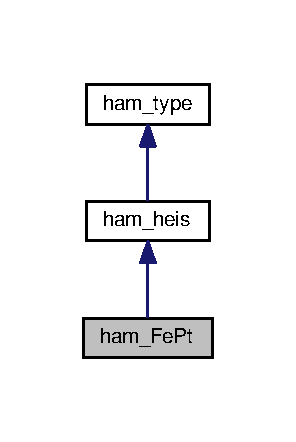
\includegraphics[width=142pt]{da/d70/classham__FePt__inherit__graph}
\end{center}
\end{figure}


Collaboration diagram for ham\+\_\+\+Fe\+Pt\+:
\nopagebreak
\begin{figure}[H]
\begin{center}
\leavevmode
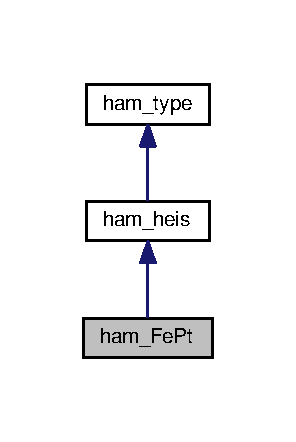
\includegraphics[width=142pt]{d8/d56/classham__FePt__coll__graph}
\end{center}
\end{figure}
\subsection*{Public Member Functions}
\begin{DoxyCompactItemize}
\item 
\hyperlink{classham__FePt_aa930e1d4953ce10685b0b593cf492bda}{ham\+\_\+\+Fe\+Pt} ()
\item 
\hyperlink{classham__FePt_ac4133bd9dcb9d80205019c245e4ca112}{ham\+\_\+\+Fe\+Pt} (double Hin)
\item 
\hyperlink{classham__FePt_a4ff7827867421f1278e953c1b58ffa99}{ham\+\_\+\+Fe\+Pt} (\hyperlink{classham__type}{ham\+\_\+type} \&other)
\item 
\hyperlink{classham__FePt_aae01414922cdaf01f0853ab167ceea56}{$\sim$ham\+\_\+\+Fe\+Pt} ()
\item 
double \hyperlink{classham__FePt_a8d69322fbb999892889d34fb4b12f043}{calc\+\_\+E} (\hyperlink{classfield__type}{field\+\_\+type} $\ast$lattice)
\item 
double \hyperlink{classham__FePt_a742137dc8f3e289bb33abb3ad04d6a19}{dE} (\hyperlink{classfield__type}{field\+\_\+type} $\ast$lattice, std\+::vector$<$ int $>$ \&position)
\item 
\hyperlink{classham__FePt}{ham\+\_\+\+Fe\+Pt} \& \hyperlink{classham__FePt_a71d6e59fb2019a3f8ec5448cd41f50c4}{operator=} (\hyperlink{classham__type}{ham\+\_\+type} \&other)
\item 
void \hyperlink{classham__FePt_ab96ff3bed5b124b8a6a7feffb075ebd9}{read\+\_\+\+Js} ()
\item 
void \hyperlink{classham__FePt_a3f03eee62cb90922ea4afea3fd1023e9}{init\+\_\+dim} (\hyperlink{classfield__type}{field\+\_\+type} $\ast$field)
\end{DoxyCompactItemize}
\subsection*{Additional Inherited Members}


\subsection{Constructor \& Destructor Documentation}
\index{ham\+\_\+\+Fe\+Pt@{ham\+\_\+\+Fe\+Pt}!ham\+\_\+\+Fe\+Pt@{ham\+\_\+\+Fe\+Pt}}
\index{ham\+\_\+\+Fe\+Pt@{ham\+\_\+\+Fe\+Pt}!ham\+\_\+\+Fe\+Pt@{ham\+\_\+\+Fe\+Pt}}
\subsubsection[{\texorpdfstring{ham\+\_\+\+Fe\+Pt()}{ham_FePt()}}]{\setlength{\rightskip}{0pt plus 5cm}ham\+\_\+\+Fe\+Pt\+::ham\+\_\+\+Fe\+Pt (
\begin{DoxyParamCaption}
{}
\end{DoxyParamCaption}
)}\hypertarget{classham__FePt_aa930e1d4953ce10685b0b593cf492bda}{}\label{classham__FePt_aa930e1d4953ce10685b0b593cf492bda}
\index{ham\+\_\+\+Fe\+Pt@{ham\+\_\+\+Fe\+Pt}!ham\+\_\+\+Fe\+Pt@{ham\+\_\+\+Fe\+Pt}}
\index{ham\+\_\+\+Fe\+Pt@{ham\+\_\+\+Fe\+Pt}!ham\+\_\+\+Fe\+Pt@{ham\+\_\+\+Fe\+Pt}}
\subsubsection[{\texorpdfstring{ham\+\_\+\+Fe\+Pt(double Hin)}{ham_FePt(double Hin)}}]{\setlength{\rightskip}{0pt plus 5cm}ham\+\_\+\+Fe\+Pt\+::ham\+\_\+\+Fe\+Pt (
\begin{DoxyParamCaption}
\item[{double}]{Hin}
\end{DoxyParamCaption}
)}\hypertarget{classham__FePt_ac4133bd9dcb9d80205019c245e4ca112}{}\label{classham__FePt_ac4133bd9dcb9d80205019c245e4ca112}
\index{ham\+\_\+\+Fe\+Pt@{ham\+\_\+\+Fe\+Pt}!ham\+\_\+\+Fe\+Pt@{ham\+\_\+\+Fe\+Pt}}
\index{ham\+\_\+\+Fe\+Pt@{ham\+\_\+\+Fe\+Pt}!ham\+\_\+\+Fe\+Pt@{ham\+\_\+\+Fe\+Pt}}
\subsubsection[{\texorpdfstring{ham\+\_\+\+Fe\+Pt(ham\+\_\+type \&other)}{ham_FePt(ham_type &other)}}]{\setlength{\rightskip}{0pt plus 5cm}ham\+\_\+\+Fe\+Pt\+::ham\+\_\+\+Fe\+Pt (
\begin{DoxyParamCaption}
\item[{{\bf ham\+\_\+type} \&}]{other}
\end{DoxyParamCaption}
)}\hypertarget{classham__FePt_a4ff7827867421f1278e953c1b58ffa99}{}\label{classham__FePt_a4ff7827867421f1278e953c1b58ffa99}
\index{ham\+\_\+\+Fe\+Pt@{ham\+\_\+\+Fe\+Pt}!````~ham\+\_\+\+Fe\+Pt@{$\sim$ham\+\_\+\+Fe\+Pt}}
\index{````~ham\+\_\+\+Fe\+Pt@{$\sim$ham\+\_\+\+Fe\+Pt}!ham\+\_\+\+Fe\+Pt@{ham\+\_\+\+Fe\+Pt}}
\subsubsection[{\texorpdfstring{$\sim$ham\+\_\+\+Fe\+Pt()}{~ham_FePt()}}]{\setlength{\rightskip}{0pt plus 5cm}ham\+\_\+\+Fe\+Pt\+::$\sim$ham\+\_\+\+Fe\+Pt (
\begin{DoxyParamCaption}
{}
\end{DoxyParamCaption}
)\hspace{0.3cm}{\ttfamily [inline]}}\hypertarget{classham__FePt_aae01414922cdaf01f0853ab167ceea56}{}\label{classham__FePt_aae01414922cdaf01f0853ab167ceea56}


\subsection{Member Function Documentation}
\index{ham\+\_\+\+Fe\+Pt@{ham\+\_\+\+Fe\+Pt}!calc\+\_\+E@{calc\+\_\+E}}
\index{calc\+\_\+E@{calc\+\_\+E}!ham\+\_\+\+Fe\+Pt@{ham\+\_\+\+Fe\+Pt}}
\subsubsection[{\texorpdfstring{calc\+\_\+\+E(field\+\_\+type $\ast$lattice)}{calc_E(field_type *lattice)}}]{\setlength{\rightskip}{0pt plus 5cm}double ham\+\_\+\+Fe\+Pt\+::calc\+\_\+E (
\begin{DoxyParamCaption}
\item[{{\bf field\+\_\+type} $\ast$}]{lattice}
\end{DoxyParamCaption}
)\hspace{0.3cm}{\ttfamily [virtual]}}\hypertarget{classham__FePt_a8d69322fbb999892889d34fb4b12f043}{}\label{classham__FePt_a8d69322fbb999892889d34fb4b12f043}


Reimplemented from \hyperlink{classham__heis_a9356396de229b2a0142fa6505f0132c1}{ham\+\_\+heis}.

\index{ham\+\_\+\+Fe\+Pt@{ham\+\_\+\+Fe\+Pt}!dE@{dE}}
\index{dE@{dE}!ham\+\_\+\+Fe\+Pt@{ham\+\_\+\+Fe\+Pt}}
\subsubsection[{\texorpdfstring{d\+E(field\+\_\+type $\ast$lattice, std\+::vector$<$ int $>$ \&position)}{dE(field_type *lattice, std::vector< int > &position)}}]{\setlength{\rightskip}{0pt plus 5cm}double ham\+\_\+\+Fe\+Pt\+::dE (
\begin{DoxyParamCaption}
\item[{{\bf field\+\_\+type} $\ast$}]{lattice, }
\item[{std\+::vector$<$ int $>$ \&}]{position}
\end{DoxyParamCaption}
)\hspace{0.3cm}{\ttfamily [virtual]}}\hypertarget{classham__FePt_a742137dc8f3e289bb33abb3ad04d6a19}{}\label{classham__FePt_a742137dc8f3e289bb33abb3ad04d6a19}


Reimplemented from \hyperlink{classham__heis_a80b17aefe298faa50b5cecb1aa9da4ad}{ham\+\_\+heis}.

\index{ham\+\_\+\+Fe\+Pt@{ham\+\_\+\+Fe\+Pt}!init\+\_\+dim@{init\+\_\+dim}}
\index{init\+\_\+dim@{init\+\_\+dim}!ham\+\_\+\+Fe\+Pt@{ham\+\_\+\+Fe\+Pt}}
\subsubsection[{\texorpdfstring{init\+\_\+dim(field\+\_\+type $\ast$field)}{init_dim(field_type *field)}}]{\setlength{\rightskip}{0pt plus 5cm}void ham\+\_\+\+Fe\+Pt\+::init\+\_\+dim (
\begin{DoxyParamCaption}
\item[{{\bf field\+\_\+type} $\ast$}]{field}
\end{DoxyParamCaption}
)\hspace{0.3cm}{\ttfamily [virtual]}}\hypertarget{classham__FePt_a3f03eee62cb90922ea4afea3fd1023e9}{}\label{classham__FePt_a3f03eee62cb90922ea4afea3fd1023e9}


Reimplemented from \hyperlink{classham__heis_a48cfb1cf4cc50765d408113878f44979}{ham\+\_\+heis}.

\index{ham\+\_\+\+Fe\+Pt@{ham\+\_\+\+Fe\+Pt}!operator=@{operator=}}
\index{operator=@{operator=}!ham\+\_\+\+Fe\+Pt@{ham\+\_\+\+Fe\+Pt}}
\subsubsection[{\texorpdfstring{operator=(ham\+\_\+type \&other)}{operator=(ham_type &other)}}]{\setlength{\rightskip}{0pt plus 5cm}{\bf ham\+\_\+\+Fe\+Pt}\& ham\+\_\+\+Fe\+Pt\+::operator= (
\begin{DoxyParamCaption}
\item[{{\bf ham\+\_\+type} \&}]{other}
\end{DoxyParamCaption}
)}\hypertarget{classham__FePt_a71d6e59fb2019a3f8ec5448cd41f50c4}{}\label{classham__FePt_a71d6e59fb2019a3f8ec5448cd41f50c4}
\index{ham\+\_\+\+Fe\+Pt@{ham\+\_\+\+Fe\+Pt}!read\+\_\+\+Js@{read\+\_\+\+Js}}
\index{read\+\_\+\+Js@{read\+\_\+\+Js}!ham\+\_\+\+Fe\+Pt@{ham\+\_\+\+Fe\+Pt}}
\subsubsection[{\texorpdfstring{read\+\_\+\+Js()}{read_Js()}}]{\setlength{\rightskip}{0pt plus 5cm}void ham\+\_\+\+Fe\+Pt\+::read\+\_\+\+Js (
\begin{DoxyParamCaption}
{}
\end{DoxyParamCaption}
)}\hypertarget{classham__FePt_ab96ff3bed5b124b8a6a7feffb075ebd9}{}\label{classham__FePt_ab96ff3bed5b124b8a6a7feffb075ebd9}


The documentation for this class was generated from the following file\+:\begin{DoxyCompactItemize}
\item 
includes/\hyperlink{hamiltonian_8hpp}{hamiltonian.\+hpp}\end{DoxyCompactItemize}

\hypertarget{classham__heis}{}\section{ham\+\_\+heis Class Reference}
\label{classham__heis}\index{ham\+\_\+heis@{ham\+\_\+heis}}


{\ttfamily \#include $<$hamiltonian.\+hpp$>$}



Inheritance diagram for ham\+\_\+heis\+:
\nopagebreak
\begin{figure}[H]
\begin{center}
\leavevmode
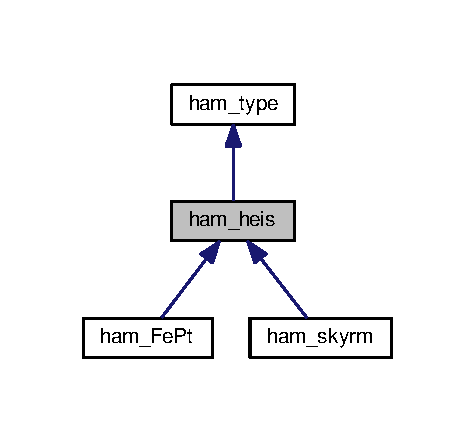
\includegraphics[width=228pt]{db/d7e/classham__heis__inherit__graph}
\end{center}
\end{figure}


Collaboration diagram for ham\+\_\+heis\+:
\nopagebreak
\begin{figure}[H]
\begin{center}
\leavevmode
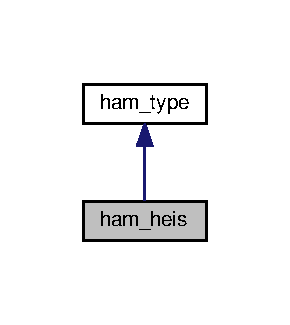
\includegraphics[width=139pt]{d0/d9a/classham__heis__coll__graph}
\end{center}
\end{figure}
\subsection*{Public Member Functions}
\begin{DoxyCompactItemize}
\item 
\hyperlink{classham__heis_a45354944ff0222eea8b2a48f3f51261b}{ham\+\_\+heis} ()
\item 
\hyperlink{classham__heis_af871854309ad6a2ec252e0af4c0d0220}{ham\+\_\+heis} (double Hin, double Jin)
\item 
\hyperlink{classham__heis_aa418d244b6fdd27e9b0c8b61d8928ee7}{ham\+\_\+heis} (\hyperlink{classham__type}{ham\+\_\+type} \&other)
\item 
\hyperlink{classham__heis_a71b4725414a6bc8f7d5ad46f86307abe}{$\sim$ham\+\_\+heis} ()
\item 
virtual double \hyperlink{classham__heis_a9356396de229b2a0142fa6505f0132c1}{calc\+\_\+E} (\hyperlink{classfield__type}{field\+\_\+type} $\ast$lattice)
\item 
std\+::vector$<$ double $>$ \hyperlink{classham__heis_ab10e4c9b74e7182751715c670cf3c44c}{calc\+\_\+M} (\hyperlink{classfield__type}{field\+\_\+type} $\ast$lattice)
\item 
std\+::vector$<$ double $>$ \hyperlink{classham__heis_a4713342c74601ac3246a34ebd429c07b}{calc\+\_\+subM} (\hyperlink{classfield__type}{field\+\_\+type} $\ast$lattice, int subnumber)
\item 
virtual double \hyperlink{classham__heis_a80b17aefe298faa50b5cecb1aa9da4ad}{dE} (\hyperlink{classfield__type}{field\+\_\+type} $\ast$lattice, std\+::vector$<$ int $>$ \&position)
\item 
std\+::vector$<$ double $>$ \hyperlink{classham__heis_a177ac16e9cc6a7b2455c0271394362af}{get\+\_\+\+Js} () const 
\item 
std\+::vector$<$ double $>$ \hyperlink{classham__heis_afbdbe29a893440db2ddab8fd41775e56}{get\+\_\+\+Hs} () const 
\item 
\hyperlink{classham__heis}{ham\+\_\+heis} \& \hyperlink{classham__heis_adc3feaa662064f07594bdbb83aef42cb}{operator=} (\hyperlink{classham__type}{ham\+\_\+type} \&other)
\item 
virtual void \hyperlink{classham__heis_a48cfb1cf4cc50765d408113878f44979}{init\+\_\+dim} (\hyperlink{classfield__type}{field\+\_\+type} $\ast$field)
\item 
void \hyperlink{classham__heis_a3c603d70b56a9df357d3c39212395422}{get\+\_\+test} (double \&x, double \&y, double \&z)
\item 
void \hyperlink{classham__heis_ab11ec994196743c909117b1231c6bfda}{set\+\_\+H} (double Hin)
\item 
std\+::vector$<$ double $>$ \hyperlink{classham__heis_a12fedc92d02868a2eacfe2e3eb2578cf}{calc\+\_\+top\+\_\+charge} (\hyperlink{classfield__type}{field\+\_\+type} $\ast$lattice)
\end{DoxyCompactItemize}
\subsection*{Protected Attributes}
\begin{DoxyCompactItemize}
\item 
std\+::vector$<$ double $>$ \hyperlink{classham__heis_af22659980108a924b51aa3b02bfce7ef}{H}
\item 
std\+::vector$<$ double $>$ \hyperlink{classham__heis_aa1cd68f7e9c6e98dd2dc9106cbb68603}{J}
\item 
double $\ast$$\ast$ \hyperlink{classham__heis_af643b0778b6c203578db1261ca3a6fd3}{adj}
\item 
std\+::vector$<$ double $>$ \hyperlink{classham__heis_ad7034ab0ac64b9c44f9975551acfc8ab}{vsum}
\item 
std\+::vector$<$ double $>$ \hyperlink{classham__heis_acbabe37ab60e2ec457106cfa49d2e1db}{curr}
\item 
std\+::vector$<$ double $>$ \hyperlink{classham__heis_a7c66e06dccb2686c392f5e9ddd8f6463}{H\+\_\+sum}
\item 
std\+::vector$<$ double $>$ \hyperlink{classham__heis_ad19fe40a32695f0f7fefb229648680b4}{J\+\_\+sum}
\item 
std\+::vector$<$ double $>$ \hyperlink{classham__heis_a5537fc1b0944509d2911fd35b4674c67}{test}
\item 
std\+::vector$<$ double $>$ \hyperlink{classham__heis_a934a89b1b1ba1a0451eced2b7398139d}{tchar}
\item 
std\+::vector$<$ double $>$ \hyperlink{classham__heis_a4b358a692afffe59e6ff0ae5255ccf30}{s2}
\item 
std\+::vector$<$ double $>$ \hyperlink{classham__heis_a50580c61051da5c6bad049c093f73a7c}{s3}
\item 
std\+::vector$<$ double $>$ \hyperlink{classham__heis_a7a09caf68e6a72d2a157e97ad23bd595}{sbuff}
\item 
std\+::vector$<$ int $>$ \hyperlink{classham__heis_afd230eba6b611edbc97677ca58b29f51}{pos}
\item 
bool \hyperlink{classham__heis_a4c756eded6f6d3e307402c02e07f82c6}{is3d}
\item 
int \hyperlink{classham__heis_a35d572f45863870d8581a83821b890ae}{tchar\+\_\+size}
\end{DoxyCompactItemize}


\subsection{Constructor \& Destructor Documentation}
\index{ham\+\_\+heis@{ham\+\_\+heis}!ham\+\_\+heis@{ham\+\_\+heis}}
\index{ham\+\_\+heis@{ham\+\_\+heis}!ham\+\_\+heis@{ham\+\_\+heis}}
\subsubsection[{\texorpdfstring{ham\+\_\+heis()}{ham_heis()}}]{\setlength{\rightskip}{0pt plus 5cm}ham\+\_\+heis\+::ham\+\_\+heis (
\begin{DoxyParamCaption}
{}
\end{DoxyParamCaption}
)\hspace{0.3cm}{\ttfamily [inline]}}\hypertarget{classham__heis_a45354944ff0222eea8b2a48f3f51261b}{}\label{classham__heis_a45354944ff0222eea8b2a48f3f51261b}
\index{ham\+\_\+heis@{ham\+\_\+heis}!ham\+\_\+heis@{ham\+\_\+heis}}
\index{ham\+\_\+heis@{ham\+\_\+heis}!ham\+\_\+heis@{ham\+\_\+heis}}
\subsubsection[{\texorpdfstring{ham\+\_\+heis(double Hin, double Jin)}{ham_heis(double Hin, double Jin)}}]{\setlength{\rightskip}{0pt plus 5cm}ham\+\_\+heis\+::ham\+\_\+heis (
\begin{DoxyParamCaption}
\item[{double}]{Hin, }
\item[{double}]{Jin}
\end{DoxyParamCaption}
)}\hypertarget{classham__heis_af871854309ad6a2ec252e0af4c0d0220}{}\label{classham__heis_af871854309ad6a2ec252e0af4c0d0220}
\index{ham\+\_\+heis@{ham\+\_\+heis}!ham\+\_\+heis@{ham\+\_\+heis}}
\index{ham\+\_\+heis@{ham\+\_\+heis}!ham\+\_\+heis@{ham\+\_\+heis}}
\subsubsection[{\texorpdfstring{ham\+\_\+heis(ham\+\_\+type \&other)}{ham_heis(ham_type &other)}}]{\setlength{\rightskip}{0pt plus 5cm}ham\+\_\+heis\+::ham\+\_\+heis (
\begin{DoxyParamCaption}
\item[{{\bf ham\+\_\+type} \&}]{other}
\end{DoxyParamCaption}
)}\hypertarget{classham__heis_aa418d244b6fdd27e9b0c8b61d8928ee7}{}\label{classham__heis_aa418d244b6fdd27e9b0c8b61d8928ee7}
\index{ham\+\_\+heis@{ham\+\_\+heis}!````~ham\+\_\+heis@{$\sim$ham\+\_\+heis}}
\index{````~ham\+\_\+heis@{$\sim$ham\+\_\+heis}!ham\+\_\+heis@{ham\+\_\+heis}}
\subsubsection[{\texorpdfstring{$\sim$ham\+\_\+heis()}{~ham_heis()}}]{\setlength{\rightskip}{0pt plus 5cm}ham\+\_\+heis\+::$\sim$ham\+\_\+heis (
\begin{DoxyParamCaption}
{}
\end{DoxyParamCaption}
)\hspace{0.3cm}{\ttfamily [inline]}}\hypertarget{classham__heis_a71b4725414a6bc8f7d5ad46f86307abe}{}\label{classham__heis_a71b4725414a6bc8f7d5ad46f86307abe}


\subsection{Member Function Documentation}
\index{ham\+\_\+heis@{ham\+\_\+heis}!calc\+\_\+E@{calc\+\_\+E}}
\index{calc\+\_\+E@{calc\+\_\+E}!ham\+\_\+heis@{ham\+\_\+heis}}
\subsubsection[{\texorpdfstring{calc\+\_\+\+E(field\+\_\+type $\ast$lattice)}{calc_E(field_type *lattice)}}]{\setlength{\rightskip}{0pt plus 5cm}virtual double ham\+\_\+heis\+::calc\+\_\+E (
\begin{DoxyParamCaption}
\item[{{\bf field\+\_\+type} $\ast$}]{lattice}
\end{DoxyParamCaption}
)\hspace{0.3cm}{\ttfamily [virtual]}}\hypertarget{classham__heis_a9356396de229b2a0142fa6505f0132c1}{}\label{classham__heis_a9356396de229b2a0142fa6505f0132c1}


Reimplemented from \hyperlink{classham__type_a7fda5d3158544255ce3ca5e20c4e1c19}{ham\+\_\+type}.



Reimplemented in \hyperlink{classham__skyrm_acca35df79a8fb4120efab41366564894}{ham\+\_\+skyrm}, and \hyperlink{classham__FePt_a8d69322fbb999892889d34fb4b12f043}{ham\+\_\+\+Fe\+Pt}.

\index{ham\+\_\+heis@{ham\+\_\+heis}!calc\+\_\+M@{calc\+\_\+M}}
\index{calc\+\_\+M@{calc\+\_\+M}!ham\+\_\+heis@{ham\+\_\+heis}}
\subsubsection[{\texorpdfstring{calc\+\_\+\+M(field\+\_\+type $\ast$lattice)}{calc_M(field_type *lattice)}}]{\setlength{\rightskip}{0pt plus 5cm}std\+::vector$<$double$>$ ham\+\_\+heis\+::calc\+\_\+M (
\begin{DoxyParamCaption}
\item[{{\bf field\+\_\+type} $\ast$}]{lattice}
\end{DoxyParamCaption}
)\hspace{0.3cm}{\ttfamily [virtual]}}\hypertarget{classham__heis_ab10e4c9b74e7182751715c670cf3c44c}{}\label{classham__heis_ab10e4c9b74e7182751715c670cf3c44c}


Reimplemented from \hyperlink{classham__type_a953ba4332e88ee644d2afb96cd5a0ad5}{ham\+\_\+type}.

\index{ham\+\_\+heis@{ham\+\_\+heis}!calc\+\_\+subM@{calc\+\_\+subM}}
\index{calc\+\_\+subM@{calc\+\_\+subM}!ham\+\_\+heis@{ham\+\_\+heis}}
\subsubsection[{\texorpdfstring{calc\+\_\+sub\+M(field\+\_\+type $\ast$lattice, int subnumber)}{calc_subM(field_type *lattice, int subnumber)}}]{\setlength{\rightskip}{0pt plus 5cm}std\+::vector$<$double$>$ ham\+\_\+heis\+::calc\+\_\+subM (
\begin{DoxyParamCaption}
\item[{{\bf field\+\_\+type} $\ast$}]{lattice, }
\item[{int}]{subnumber}
\end{DoxyParamCaption}
)\hspace{0.3cm}{\ttfamily [virtual]}}\hypertarget{classham__heis_a4713342c74601ac3246a34ebd429c07b}{}\label{classham__heis_a4713342c74601ac3246a34ebd429c07b}


Reimplemented from \hyperlink{classham__type_a37cc0a51074bd64cdeec866edb6f6015}{ham\+\_\+type}.

\index{ham\+\_\+heis@{ham\+\_\+heis}!calc\+\_\+top\+\_\+charge@{calc\+\_\+top\+\_\+charge}}
\index{calc\+\_\+top\+\_\+charge@{calc\+\_\+top\+\_\+charge}!ham\+\_\+heis@{ham\+\_\+heis}}
\subsubsection[{\texorpdfstring{calc\+\_\+top\+\_\+charge(field\+\_\+type $\ast$lattice)}{calc_top_charge(field_type *lattice)}}]{\setlength{\rightskip}{0pt plus 5cm}std\+::vector$<$double$>$ ham\+\_\+heis\+::calc\+\_\+top\+\_\+charge (
\begin{DoxyParamCaption}
\item[{{\bf field\+\_\+type} $\ast$}]{lattice}
\end{DoxyParamCaption}
)\hspace{0.3cm}{\ttfamily [virtual]}}\hypertarget{classham__heis_a12fedc92d02868a2eacfe2e3eb2578cf}{}\label{classham__heis_a12fedc92d02868a2eacfe2e3eb2578cf}


Reimplemented from \hyperlink{classham__type_ab6917097da83d4855efe2238ab4df4da}{ham\+\_\+type}.

\index{ham\+\_\+heis@{ham\+\_\+heis}!dE@{dE}}
\index{dE@{dE}!ham\+\_\+heis@{ham\+\_\+heis}}
\subsubsection[{\texorpdfstring{d\+E(field\+\_\+type $\ast$lattice, std\+::vector$<$ int $>$ \&position)}{dE(field_type *lattice, std::vector< int > &position)}}]{\setlength{\rightskip}{0pt plus 5cm}virtual double ham\+\_\+heis\+::dE (
\begin{DoxyParamCaption}
\item[{{\bf field\+\_\+type} $\ast$}]{lattice, }
\item[{std\+::vector$<$ int $>$ \&}]{position}
\end{DoxyParamCaption}
)\hspace{0.3cm}{\ttfamily [virtual]}}\hypertarget{classham__heis_a80b17aefe298faa50b5cecb1aa9da4ad}{}\label{classham__heis_a80b17aefe298faa50b5cecb1aa9da4ad}


Reimplemented from \hyperlink{classham__type_a809902357229189b08ee9fdfab9c90be}{ham\+\_\+type}.



Reimplemented in \hyperlink{classham__skyrm_aca80743449de874029fc0860fdd36422}{ham\+\_\+skyrm}, and \hyperlink{classham__FePt_a742137dc8f3e289bb33abb3ad04d6a19}{ham\+\_\+\+Fe\+Pt}.

\index{ham\+\_\+heis@{ham\+\_\+heis}!get\+\_\+\+Hs@{get\+\_\+\+Hs}}
\index{get\+\_\+\+Hs@{get\+\_\+\+Hs}!ham\+\_\+heis@{ham\+\_\+heis}}
\subsubsection[{\texorpdfstring{get\+\_\+\+Hs() const }{get_Hs() const }}]{\setlength{\rightskip}{0pt plus 5cm}std\+::vector$<$double$>$ ham\+\_\+heis\+::get\+\_\+\+Hs (
\begin{DoxyParamCaption}
{}
\end{DoxyParamCaption}
) const\hspace{0.3cm}{\ttfamily [inline]}, {\ttfamily [virtual]}}\hypertarget{classham__heis_afbdbe29a893440db2ddab8fd41775e56}{}\label{classham__heis_afbdbe29a893440db2ddab8fd41775e56}


Reimplemented from \hyperlink{classham__type_aab0cee1eece99ec37122126e7e4bcb91}{ham\+\_\+type}.

\index{ham\+\_\+heis@{ham\+\_\+heis}!get\+\_\+\+Js@{get\+\_\+\+Js}}
\index{get\+\_\+\+Js@{get\+\_\+\+Js}!ham\+\_\+heis@{ham\+\_\+heis}}
\subsubsection[{\texorpdfstring{get\+\_\+\+Js() const }{get_Js() const }}]{\setlength{\rightskip}{0pt plus 5cm}std\+::vector$<$double$>$ ham\+\_\+heis\+::get\+\_\+\+Js (
\begin{DoxyParamCaption}
{}
\end{DoxyParamCaption}
) const\hspace{0.3cm}{\ttfamily [inline]}, {\ttfamily [virtual]}}\hypertarget{classham__heis_a177ac16e9cc6a7b2455c0271394362af}{}\label{classham__heis_a177ac16e9cc6a7b2455c0271394362af}


Reimplemented from \hyperlink{classham__type_accdb77a4f5af92232a0415212d302344}{ham\+\_\+type}.

\index{ham\+\_\+heis@{ham\+\_\+heis}!get\+\_\+test@{get\+\_\+test}}
\index{get\+\_\+test@{get\+\_\+test}!ham\+\_\+heis@{ham\+\_\+heis}}
\subsubsection[{\texorpdfstring{get\+\_\+test(double \&x, double \&y, double \&z)}{get_test(double &x, double &y, double &z)}}]{\setlength{\rightskip}{0pt plus 5cm}void ham\+\_\+heis\+::get\+\_\+test (
\begin{DoxyParamCaption}
\item[{double \&}]{x, }
\item[{double \&}]{y, }
\item[{double \&}]{z}
\end{DoxyParamCaption}
)\hspace{0.3cm}{\ttfamily [inline]}, {\ttfamily [virtual]}}\hypertarget{classham__heis_a3c603d70b56a9df357d3c39212395422}{}\label{classham__heis_a3c603d70b56a9df357d3c39212395422}


Reimplemented from \hyperlink{classham__type_a2864138405e794dc2aa2fe45fb6e400f}{ham\+\_\+type}.

\index{ham\+\_\+heis@{ham\+\_\+heis}!init\+\_\+dim@{init\+\_\+dim}}
\index{init\+\_\+dim@{init\+\_\+dim}!ham\+\_\+heis@{ham\+\_\+heis}}
\subsubsection[{\texorpdfstring{init\+\_\+dim(field\+\_\+type $\ast$field)}{init_dim(field_type *field)}}]{\setlength{\rightskip}{0pt plus 5cm}virtual void ham\+\_\+heis\+::init\+\_\+dim (
\begin{DoxyParamCaption}
\item[{{\bf field\+\_\+type} $\ast$}]{field}
\end{DoxyParamCaption}
)\hspace{0.3cm}{\ttfamily [virtual]}}\hypertarget{classham__heis_a48cfb1cf4cc50765d408113878f44979}{}\label{classham__heis_a48cfb1cf4cc50765d408113878f44979}


Reimplemented from \hyperlink{classham__type_a3a14214575bf8dcf3a8b39c7470dfe66}{ham\+\_\+type}.



Reimplemented in \hyperlink{classham__FePt_a3f03eee62cb90922ea4afea3fd1023e9}{ham\+\_\+\+Fe\+Pt}.

\index{ham\+\_\+heis@{ham\+\_\+heis}!operator=@{operator=}}
\index{operator=@{operator=}!ham\+\_\+heis@{ham\+\_\+heis}}
\subsubsection[{\texorpdfstring{operator=(ham\+\_\+type \&other)}{operator=(ham_type &other)}}]{\setlength{\rightskip}{0pt plus 5cm}{\bf ham\+\_\+heis}\& ham\+\_\+heis\+::operator= (
\begin{DoxyParamCaption}
\item[{{\bf ham\+\_\+type} \&}]{other}
\end{DoxyParamCaption}
)}\hypertarget{classham__heis_adc3feaa662064f07594bdbb83aef42cb}{}\label{classham__heis_adc3feaa662064f07594bdbb83aef42cb}
\index{ham\+\_\+heis@{ham\+\_\+heis}!set\+\_\+H@{set\+\_\+H}}
\index{set\+\_\+H@{set\+\_\+H}!ham\+\_\+heis@{ham\+\_\+heis}}
\subsubsection[{\texorpdfstring{set\+\_\+\+H(double Hin)}{set_H(double Hin)}}]{\setlength{\rightskip}{0pt plus 5cm}void ham\+\_\+heis\+::set\+\_\+H (
\begin{DoxyParamCaption}
\item[{double}]{Hin}
\end{DoxyParamCaption}
)\hspace{0.3cm}{\ttfamily [inline]}, {\ttfamily [virtual]}}\hypertarget{classham__heis_ab11ec994196743c909117b1231c6bfda}{}\label{classham__heis_ab11ec994196743c909117b1231c6bfda}


Reimplemented from \hyperlink{classham__type_a140c53e29c5c298c0f2704a4ecda7022}{ham\+\_\+type}.



\subsection{Member Data Documentation}
\index{ham\+\_\+heis@{ham\+\_\+heis}!adj@{adj}}
\index{adj@{adj}!ham\+\_\+heis@{ham\+\_\+heis}}
\subsubsection[{\texorpdfstring{adj}{adj}}]{\setlength{\rightskip}{0pt plus 5cm}double$\ast$$\ast$ ham\+\_\+heis\+::adj\hspace{0.3cm}{\ttfamily [protected]}}\hypertarget{classham__heis_af643b0778b6c203578db1261ca3a6fd3}{}\label{classham__heis_af643b0778b6c203578db1261ca3a6fd3}
\index{ham\+\_\+heis@{ham\+\_\+heis}!curr@{curr}}
\index{curr@{curr}!ham\+\_\+heis@{ham\+\_\+heis}}
\subsubsection[{\texorpdfstring{curr}{curr}}]{\setlength{\rightskip}{0pt plus 5cm}std\+::vector$<$double$>$ ham\+\_\+heis\+::curr\hspace{0.3cm}{\ttfamily [protected]}}\hypertarget{classham__heis_acbabe37ab60e2ec457106cfa49d2e1db}{}\label{classham__heis_acbabe37ab60e2ec457106cfa49d2e1db}
\index{ham\+\_\+heis@{ham\+\_\+heis}!H@{H}}
\index{H@{H}!ham\+\_\+heis@{ham\+\_\+heis}}
\subsubsection[{\texorpdfstring{H}{H}}]{\setlength{\rightskip}{0pt plus 5cm}std\+::vector$<$double$>$ ham\+\_\+heis\+::H\hspace{0.3cm}{\ttfamily [protected]}}\hypertarget{classham__heis_af22659980108a924b51aa3b02bfce7ef}{}\label{classham__heis_af22659980108a924b51aa3b02bfce7ef}
\index{ham\+\_\+heis@{ham\+\_\+heis}!H\+\_\+sum@{H\+\_\+sum}}
\index{H\+\_\+sum@{H\+\_\+sum}!ham\+\_\+heis@{ham\+\_\+heis}}
\subsubsection[{\texorpdfstring{H\+\_\+sum}{H_sum}}]{\setlength{\rightskip}{0pt plus 5cm}std\+::vector$<$double$>$ ham\+\_\+heis\+::\+H\+\_\+sum\hspace{0.3cm}{\ttfamily [protected]}}\hypertarget{classham__heis_a7c66e06dccb2686c392f5e9ddd8f6463}{}\label{classham__heis_a7c66e06dccb2686c392f5e9ddd8f6463}
\index{ham\+\_\+heis@{ham\+\_\+heis}!is3d@{is3d}}
\index{is3d@{is3d}!ham\+\_\+heis@{ham\+\_\+heis}}
\subsubsection[{\texorpdfstring{is3d}{is3d}}]{\setlength{\rightskip}{0pt plus 5cm}bool ham\+\_\+heis\+::is3d\hspace{0.3cm}{\ttfamily [protected]}}\hypertarget{classham__heis_a4c756eded6f6d3e307402c02e07f82c6}{}\label{classham__heis_a4c756eded6f6d3e307402c02e07f82c6}
\index{ham\+\_\+heis@{ham\+\_\+heis}!J@{J}}
\index{J@{J}!ham\+\_\+heis@{ham\+\_\+heis}}
\subsubsection[{\texorpdfstring{J}{J}}]{\setlength{\rightskip}{0pt plus 5cm}std\+::vector$<$double$>$ ham\+\_\+heis\+::J\hspace{0.3cm}{\ttfamily [protected]}}\hypertarget{classham__heis_aa1cd68f7e9c6e98dd2dc9106cbb68603}{}\label{classham__heis_aa1cd68f7e9c6e98dd2dc9106cbb68603}
\index{ham\+\_\+heis@{ham\+\_\+heis}!J\+\_\+sum@{J\+\_\+sum}}
\index{J\+\_\+sum@{J\+\_\+sum}!ham\+\_\+heis@{ham\+\_\+heis}}
\subsubsection[{\texorpdfstring{J\+\_\+sum}{J_sum}}]{\setlength{\rightskip}{0pt plus 5cm}std\+::vector$<$double$>$ ham\+\_\+heis\+::\+J\+\_\+sum\hspace{0.3cm}{\ttfamily [protected]}}\hypertarget{classham__heis_ad19fe40a32695f0f7fefb229648680b4}{}\label{classham__heis_ad19fe40a32695f0f7fefb229648680b4}
\index{ham\+\_\+heis@{ham\+\_\+heis}!pos@{pos}}
\index{pos@{pos}!ham\+\_\+heis@{ham\+\_\+heis}}
\subsubsection[{\texorpdfstring{pos}{pos}}]{\setlength{\rightskip}{0pt plus 5cm}std\+::vector$<$int$>$ ham\+\_\+heis\+::pos\hspace{0.3cm}{\ttfamily [protected]}}\hypertarget{classham__heis_afd230eba6b611edbc97677ca58b29f51}{}\label{classham__heis_afd230eba6b611edbc97677ca58b29f51}
\index{ham\+\_\+heis@{ham\+\_\+heis}!s2@{s2}}
\index{s2@{s2}!ham\+\_\+heis@{ham\+\_\+heis}}
\subsubsection[{\texorpdfstring{s2}{s2}}]{\setlength{\rightskip}{0pt plus 5cm}std\+::vector$<$double$>$ ham\+\_\+heis\+::s2\hspace{0.3cm}{\ttfamily [protected]}}\hypertarget{classham__heis_a4b358a692afffe59e6ff0ae5255ccf30}{}\label{classham__heis_a4b358a692afffe59e6ff0ae5255ccf30}
\index{ham\+\_\+heis@{ham\+\_\+heis}!s3@{s3}}
\index{s3@{s3}!ham\+\_\+heis@{ham\+\_\+heis}}
\subsubsection[{\texorpdfstring{s3}{s3}}]{\setlength{\rightskip}{0pt plus 5cm}std\+::vector$<$double$>$ ham\+\_\+heis\+::s3\hspace{0.3cm}{\ttfamily [protected]}}\hypertarget{classham__heis_a50580c61051da5c6bad049c093f73a7c}{}\label{classham__heis_a50580c61051da5c6bad049c093f73a7c}
\index{ham\+\_\+heis@{ham\+\_\+heis}!sbuff@{sbuff}}
\index{sbuff@{sbuff}!ham\+\_\+heis@{ham\+\_\+heis}}
\subsubsection[{\texorpdfstring{sbuff}{sbuff}}]{\setlength{\rightskip}{0pt plus 5cm}std\+::vector$<$double$>$ ham\+\_\+heis\+::sbuff\hspace{0.3cm}{\ttfamily [protected]}}\hypertarget{classham__heis_a7a09caf68e6a72d2a157e97ad23bd595}{}\label{classham__heis_a7a09caf68e6a72d2a157e97ad23bd595}
\index{ham\+\_\+heis@{ham\+\_\+heis}!tchar@{tchar}}
\index{tchar@{tchar}!ham\+\_\+heis@{ham\+\_\+heis}}
\subsubsection[{\texorpdfstring{tchar}{tchar}}]{\setlength{\rightskip}{0pt plus 5cm}std\+::vector$<$double$>$ ham\+\_\+heis\+::tchar\hspace{0.3cm}{\ttfamily [protected]}}\hypertarget{classham__heis_a934a89b1b1ba1a0451eced2b7398139d}{}\label{classham__heis_a934a89b1b1ba1a0451eced2b7398139d}
\index{ham\+\_\+heis@{ham\+\_\+heis}!tchar\+\_\+size@{tchar\+\_\+size}}
\index{tchar\+\_\+size@{tchar\+\_\+size}!ham\+\_\+heis@{ham\+\_\+heis}}
\subsubsection[{\texorpdfstring{tchar\+\_\+size}{tchar_size}}]{\setlength{\rightskip}{0pt plus 5cm}int ham\+\_\+heis\+::tchar\+\_\+size\hspace{0.3cm}{\ttfamily [protected]}}\hypertarget{classham__heis_a35d572f45863870d8581a83821b890ae}{}\label{classham__heis_a35d572f45863870d8581a83821b890ae}
\index{ham\+\_\+heis@{ham\+\_\+heis}!test@{test}}
\index{test@{test}!ham\+\_\+heis@{ham\+\_\+heis}}
\subsubsection[{\texorpdfstring{test}{test}}]{\setlength{\rightskip}{0pt plus 5cm}std\+::vector$<$double$>$ ham\+\_\+heis\+::test\hspace{0.3cm}{\ttfamily [protected]}}\hypertarget{classham__heis_a5537fc1b0944509d2911fd35b4674c67}{}\label{classham__heis_a5537fc1b0944509d2911fd35b4674c67}
\index{ham\+\_\+heis@{ham\+\_\+heis}!vsum@{vsum}}
\index{vsum@{vsum}!ham\+\_\+heis@{ham\+\_\+heis}}
\subsubsection[{\texorpdfstring{vsum}{vsum}}]{\setlength{\rightskip}{0pt plus 5cm}std\+::vector$<$double$>$ ham\+\_\+heis\+::vsum\hspace{0.3cm}{\ttfamily [protected]}}\hypertarget{classham__heis_ad7034ab0ac64b9c44f9975551acfc8ab}{}\label{classham__heis_ad7034ab0ac64b9c44f9975551acfc8ab}


The documentation for this class was generated from the following file\+:\begin{DoxyCompactItemize}
\item 
includes/\hyperlink{hamiltonian_8hpp}{hamiltonian.\+hpp}\end{DoxyCompactItemize}

\hypertarget{classham__ising}{}\section{ham\+\_\+ising Class Reference}
\label{classham__ising}\index{ham\+\_\+ising@{ham\+\_\+ising}}


{\ttfamily \#include $<$hamiltonian.\+hpp$>$}



Inheritance diagram for ham\+\_\+ising\+:
\nopagebreak
\begin{figure}[H]
\begin{center}
\leavevmode
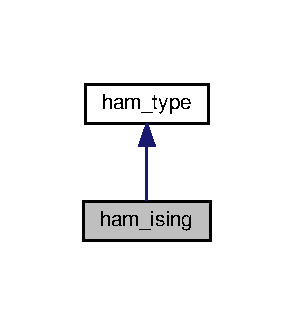
\includegraphics[width=141pt]{d1/de5/classham__ising__inherit__graph}
\end{center}
\end{figure}


Collaboration diagram for ham\+\_\+ising\+:
\nopagebreak
\begin{figure}[H]
\begin{center}
\leavevmode
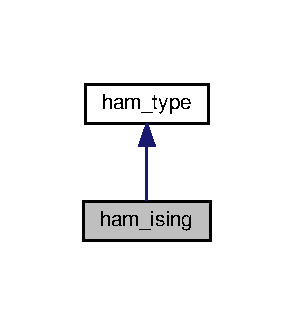
\includegraphics[width=141pt]{d7/d27/classham__ising__coll__graph}
\end{center}
\end{figure}
\subsection*{Public Member Functions}
\begin{DoxyCompactItemize}
\item 
\hyperlink{classham__ising_a7d8f84c23bfdc73ff1ae9802f301b4ac}{ham\+\_\+ising} ()
\item 
\hyperlink{classham__ising_a78b0da58aa8aa9d45a34cbcab0758321}{ham\+\_\+ising} (double Hin, double Jin)
\item 
\hyperlink{classham__ising_a89452c56f4810fbd26807be64936048a}{ham\+\_\+ising} (\hyperlink{classham__type}{ham\+\_\+type} \&other)
\item 
\hyperlink{classham__ising_ab8232cf72719703d5392e960f24996f0}{$\sim$ham\+\_\+ising} ()
\item 
double \hyperlink{classham__ising_a04bdf2c223bada94ca813bc71d71e7cb}{calc\+\_\+E} (\hyperlink{classfield__type}{field\+\_\+type} $\ast$lattice)
\item 
std\+::vector$<$ double $>$ \hyperlink{classham__ising_ad530e522cb6a2a80d10948603ff667ff}{calc\+\_\+M} (\hyperlink{classfield__type}{field\+\_\+type} $\ast$lattice)
\item 
std\+::vector$<$ double $>$ \hyperlink{classham__ising_a7092d807838fed1640bb03fa22e71236}{calc\+\_\+subM} (\hyperlink{classfield__type}{field\+\_\+type} $\ast$lattice, int subnumber)
\item 
double \hyperlink{classham__ising_ae83e5c08a8da4652440ccd5d40554421}{dE} (\hyperlink{classfield__type}{field\+\_\+type} $\ast$lattice, std\+::vector$<$ int $>$ \&position)
\item 
double \hyperlink{classham__ising_a3d5b100c6f3a1f750c524a2d302fd65e}{get\+\_\+J} () const 
\item 
double \hyperlink{classham__ising_aa03103158f5db829b8f17f43978a816c}{get\+\_\+H} () const 
\item 
\hyperlink{classham__ising}{ham\+\_\+ising} \& \hyperlink{classham__ising_a19a91ce13ee2834f11aea703b335a1da}{operator=} (\hyperlink{classham__type}{ham\+\_\+type} \&other)
\item 
void \hyperlink{classham__ising_a92139385ee5cd3eab8a03897245dc53f}{init\+\_\+dim} (\hyperlink{classfield__type}{field\+\_\+type} $\ast$field)
\item 
void \hyperlink{classham__ising_a4b0bdb0e5576905061ec607cbeeb76cb}{set\+\_\+H} (double Hin)
\end{DoxyCompactItemize}
\subsection*{Additional Inherited Members}


\subsection{Constructor \& Destructor Documentation}
\index{ham\+\_\+ising@{ham\+\_\+ising}!ham\+\_\+ising@{ham\+\_\+ising}}
\index{ham\+\_\+ising@{ham\+\_\+ising}!ham\+\_\+ising@{ham\+\_\+ising}}
\subsubsection[{\texorpdfstring{ham\+\_\+ising()}{ham_ising()}}]{\setlength{\rightskip}{0pt plus 5cm}ham\+\_\+ising\+::ham\+\_\+ising (
\begin{DoxyParamCaption}
{}
\end{DoxyParamCaption}
)\hspace{0.3cm}{\ttfamily [inline]}}\hypertarget{classham__ising_a7d8f84c23bfdc73ff1ae9802f301b4ac}{}\label{classham__ising_a7d8f84c23bfdc73ff1ae9802f301b4ac}
\index{ham\+\_\+ising@{ham\+\_\+ising}!ham\+\_\+ising@{ham\+\_\+ising}}
\index{ham\+\_\+ising@{ham\+\_\+ising}!ham\+\_\+ising@{ham\+\_\+ising}}
\subsubsection[{\texorpdfstring{ham\+\_\+ising(double Hin, double Jin)}{ham_ising(double Hin, double Jin)}}]{\setlength{\rightskip}{0pt plus 5cm}ham\+\_\+ising\+::ham\+\_\+ising (
\begin{DoxyParamCaption}
\item[{double}]{Hin, }
\item[{double}]{Jin}
\end{DoxyParamCaption}
)\hspace{0.3cm}{\ttfamily [inline]}}\hypertarget{classham__ising_a78b0da58aa8aa9d45a34cbcab0758321}{}\label{classham__ising_a78b0da58aa8aa9d45a34cbcab0758321}
\index{ham\+\_\+ising@{ham\+\_\+ising}!ham\+\_\+ising@{ham\+\_\+ising}}
\index{ham\+\_\+ising@{ham\+\_\+ising}!ham\+\_\+ising@{ham\+\_\+ising}}
\subsubsection[{\texorpdfstring{ham\+\_\+ising(ham\+\_\+type \&other)}{ham_ising(ham_type &other)}}]{\setlength{\rightskip}{0pt plus 5cm}ham\+\_\+ising\+::ham\+\_\+ising (
\begin{DoxyParamCaption}
\item[{{\bf ham\+\_\+type} \&}]{other}
\end{DoxyParamCaption}
)}\hypertarget{classham__ising_a89452c56f4810fbd26807be64936048a}{}\label{classham__ising_a89452c56f4810fbd26807be64936048a}
\index{ham\+\_\+ising@{ham\+\_\+ising}!````~ham\+\_\+ising@{$\sim$ham\+\_\+ising}}
\index{````~ham\+\_\+ising@{$\sim$ham\+\_\+ising}!ham\+\_\+ising@{ham\+\_\+ising}}
\subsubsection[{\texorpdfstring{$\sim$ham\+\_\+ising()}{~ham_ising()}}]{\setlength{\rightskip}{0pt plus 5cm}ham\+\_\+ising\+::$\sim$ham\+\_\+ising (
\begin{DoxyParamCaption}
{}
\end{DoxyParamCaption}
)\hspace{0.3cm}{\ttfamily [inline]}}\hypertarget{classham__ising_ab8232cf72719703d5392e960f24996f0}{}\label{classham__ising_ab8232cf72719703d5392e960f24996f0}


\subsection{Member Function Documentation}
\index{ham\+\_\+ising@{ham\+\_\+ising}!calc\+\_\+E@{calc\+\_\+E}}
\index{calc\+\_\+E@{calc\+\_\+E}!ham\+\_\+ising@{ham\+\_\+ising}}
\subsubsection[{\texorpdfstring{calc\+\_\+\+E(field\+\_\+type $\ast$lattice)}{calc_E(field_type *lattice)}}]{\setlength{\rightskip}{0pt plus 5cm}double ham\+\_\+ising\+::calc\+\_\+E (
\begin{DoxyParamCaption}
\item[{{\bf field\+\_\+type} $\ast$}]{lattice}
\end{DoxyParamCaption}
)\hspace{0.3cm}{\ttfamily [virtual]}}\hypertarget{classham__ising_a04bdf2c223bada94ca813bc71d71e7cb}{}\label{classham__ising_a04bdf2c223bada94ca813bc71d71e7cb}


Reimplemented from \hyperlink{classham__type_a7fda5d3158544255ce3ca5e20c4e1c19}{ham\+\_\+type}.

\index{ham\+\_\+ising@{ham\+\_\+ising}!calc\+\_\+M@{calc\+\_\+M}}
\index{calc\+\_\+M@{calc\+\_\+M}!ham\+\_\+ising@{ham\+\_\+ising}}
\subsubsection[{\texorpdfstring{calc\+\_\+\+M(field\+\_\+type $\ast$lattice)}{calc_M(field_type *lattice)}}]{\setlength{\rightskip}{0pt plus 5cm}std\+::vector$<$double$>$ ham\+\_\+ising\+::calc\+\_\+M (
\begin{DoxyParamCaption}
\item[{{\bf field\+\_\+type} $\ast$}]{lattice}
\end{DoxyParamCaption}
)\hspace{0.3cm}{\ttfamily [virtual]}}\hypertarget{classham__ising_ad530e522cb6a2a80d10948603ff667ff}{}\label{classham__ising_ad530e522cb6a2a80d10948603ff667ff}


Reimplemented from \hyperlink{classham__type_a953ba4332e88ee644d2afb96cd5a0ad5}{ham\+\_\+type}.

\index{ham\+\_\+ising@{ham\+\_\+ising}!calc\+\_\+subM@{calc\+\_\+subM}}
\index{calc\+\_\+subM@{calc\+\_\+subM}!ham\+\_\+ising@{ham\+\_\+ising}}
\subsubsection[{\texorpdfstring{calc\+\_\+sub\+M(field\+\_\+type $\ast$lattice, int subnumber)}{calc_subM(field_type *lattice, int subnumber)}}]{\setlength{\rightskip}{0pt plus 5cm}std\+::vector$<$double$>$ ham\+\_\+ising\+::calc\+\_\+subM (
\begin{DoxyParamCaption}
\item[{{\bf field\+\_\+type} $\ast$}]{lattice, }
\item[{int}]{subnumber}
\end{DoxyParamCaption}
)\hspace{0.3cm}{\ttfamily [virtual]}}\hypertarget{classham__ising_a7092d807838fed1640bb03fa22e71236}{}\label{classham__ising_a7092d807838fed1640bb03fa22e71236}


Reimplemented from \hyperlink{classham__type_a37cc0a51074bd64cdeec866edb6f6015}{ham\+\_\+type}.

\index{ham\+\_\+ising@{ham\+\_\+ising}!dE@{dE}}
\index{dE@{dE}!ham\+\_\+ising@{ham\+\_\+ising}}
\subsubsection[{\texorpdfstring{d\+E(field\+\_\+type $\ast$lattice, std\+::vector$<$ int $>$ \&position)}{dE(field_type *lattice, std::vector< int > &position)}}]{\setlength{\rightskip}{0pt plus 5cm}double ham\+\_\+ising\+::dE (
\begin{DoxyParamCaption}
\item[{{\bf field\+\_\+type} $\ast$}]{lattice, }
\item[{std\+::vector$<$ int $>$ \&}]{position}
\end{DoxyParamCaption}
)\hspace{0.3cm}{\ttfamily [virtual]}}\hypertarget{classham__ising_ae83e5c08a8da4652440ccd5d40554421}{}\label{classham__ising_ae83e5c08a8da4652440ccd5d40554421}


Reimplemented from \hyperlink{classham__type_a809902357229189b08ee9fdfab9c90be}{ham\+\_\+type}.

\index{ham\+\_\+ising@{ham\+\_\+ising}!get\+\_\+H@{get\+\_\+H}}
\index{get\+\_\+H@{get\+\_\+H}!ham\+\_\+ising@{ham\+\_\+ising}}
\subsubsection[{\texorpdfstring{get\+\_\+\+H() const }{get_H() const }}]{\setlength{\rightskip}{0pt plus 5cm}double ham\+\_\+ising\+::get\+\_\+H (
\begin{DoxyParamCaption}
{}
\end{DoxyParamCaption}
) const\hspace{0.3cm}{\ttfamily [inline]}, {\ttfamily [virtual]}}\hypertarget{classham__ising_aa03103158f5db829b8f17f43978a816c}{}\label{classham__ising_aa03103158f5db829b8f17f43978a816c}


Reimplemented from \hyperlink{classham__type_a1c1a0ee7708f3d6f68bc999491dde42b}{ham\+\_\+type}.

\index{ham\+\_\+ising@{ham\+\_\+ising}!get\+\_\+J@{get\+\_\+J}}
\index{get\+\_\+J@{get\+\_\+J}!ham\+\_\+ising@{ham\+\_\+ising}}
\subsubsection[{\texorpdfstring{get\+\_\+\+J() const }{get_J() const }}]{\setlength{\rightskip}{0pt plus 5cm}double ham\+\_\+ising\+::get\+\_\+J (
\begin{DoxyParamCaption}
{}
\end{DoxyParamCaption}
) const\hspace{0.3cm}{\ttfamily [inline]}, {\ttfamily [virtual]}}\hypertarget{classham__ising_a3d5b100c6f3a1f750c524a2d302fd65e}{}\label{classham__ising_a3d5b100c6f3a1f750c524a2d302fd65e}


Reimplemented from \hyperlink{classham__type_ab75b9c6ea8098ea0874781a70bfa5099}{ham\+\_\+type}.

\index{ham\+\_\+ising@{ham\+\_\+ising}!init\+\_\+dim@{init\+\_\+dim}}
\index{init\+\_\+dim@{init\+\_\+dim}!ham\+\_\+ising@{ham\+\_\+ising}}
\subsubsection[{\texorpdfstring{init\+\_\+dim(field\+\_\+type $\ast$field)}{init_dim(field_type *field)}}]{\setlength{\rightskip}{0pt plus 5cm}void ham\+\_\+ising\+::init\+\_\+dim (
\begin{DoxyParamCaption}
\item[{{\bf field\+\_\+type} $\ast$}]{field}
\end{DoxyParamCaption}
)\hspace{0.3cm}{\ttfamily [virtual]}}\hypertarget{classham__ising_a92139385ee5cd3eab8a03897245dc53f}{}\label{classham__ising_a92139385ee5cd3eab8a03897245dc53f}


Reimplemented from \hyperlink{classham__type_a3a14214575bf8dcf3a8b39c7470dfe66}{ham\+\_\+type}.

\index{ham\+\_\+ising@{ham\+\_\+ising}!operator=@{operator=}}
\index{operator=@{operator=}!ham\+\_\+ising@{ham\+\_\+ising}}
\subsubsection[{\texorpdfstring{operator=(ham\+\_\+type \&other)}{operator=(ham_type &other)}}]{\setlength{\rightskip}{0pt plus 5cm}{\bf ham\+\_\+ising}\& ham\+\_\+ising\+::operator= (
\begin{DoxyParamCaption}
\item[{{\bf ham\+\_\+type} \&}]{other}
\end{DoxyParamCaption}
)}\hypertarget{classham__ising_a19a91ce13ee2834f11aea703b335a1da}{}\label{classham__ising_a19a91ce13ee2834f11aea703b335a1da}
\index{ham\+\_\+ising@{ham\+\_\+ising}!set\+\_\+H@{set\+\_\+H}}
\index{set\+\_\+H@{set\+\_\+H}!ham\+\_\+ising@{ham\+\_\+ising}}
\subsubsection[{\texorpdfstring{set\+\_\+\+H(double Hin)}{set_H(double Hin)}}]{\setlength{\rightskip}{0pt plus 5cm}void ham\+\_\+ising\+::set\+\_\+H (
\begin{DoxyParamCaption}
\item[{double}]{Hin}
\end{DoxyParamCaption}
)\hspace{0.3cm}{\ttfamily [inline]}, {\ttfamily [virtual]}}\hypertarget{classham__ising_a4b0bdb0e5576905061ec607cbeeb76cb}{}\label{classham__ising_a4b0bdb0e5576905061ec607cbeeb76cb}


Reimplemented from \hyperlink{classham__type_a140c53e29c5c298c0f2704a4ecda7022}{ham\+\_\+type}.



The documentation for this class was generated from the following file\+:\begin{DoxyCompactItemize}
\item 
includes/\hyperlink{hamiltonian_8hpp}{hamiltonian.\+hpp}\end{DoxyCompactItemize}

\hypertarget{classham__skyrm}{}\section{ham\+\_\+skyrm Class Reference}
\label{classham__skyrm}\index{ham\+\_\+skyrm@{ham\+\_\+skyrm}}


{\ttfamily \#include $<$hamiltonian.\+hpp$>$}



Inheritance diagram for ham\+\_\+skyrm\+:\nopagebreak
\begin{figure}[H]
\begin{center}
\leavevmode
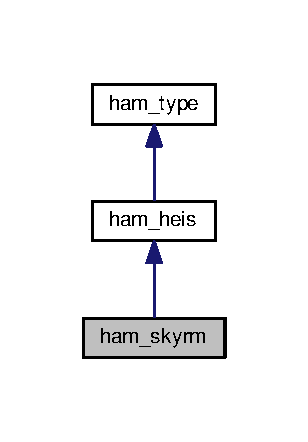
\includegraphics[width=148pt]{d0/d5b/classham__skyrm__inherit__graph}
\end{center}
\end{figure}


Collaboration diagram for ham\+\_\+skyrm\+:\nopagebreak
\begin{figure}[H]
\begin{center}
\leavevmode
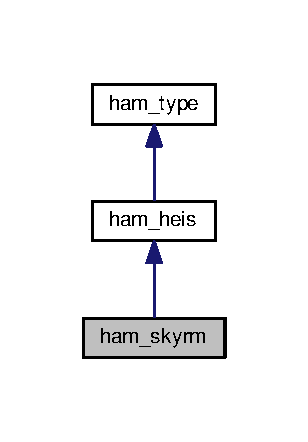
\includegraphics[width=148pt]{d6/d7d/classham__skyrm__coll__graph}
\end{center}
\end{figure}
\subsection*{Public Member Functions}
\begin{DoxyCompactItemize}
\item 
\hyperlink{classham__skyrm_a998679f07f8bb5f1e130f9aa2c839026}{ham\+\_\+skyrm} ()
\item 
\hyperlink{classham__skyrm_a75b7e0c02042d8560ee8b10157985b42}{ham\+\_\+skyrm} (double Hin, double Jin, double Kin)
\item 
\hyperlink{classham__skyrm_a8714765903ae11e6da673d7c5b4ef8fd}{ham\+\_\+skyrm} (const \hyperlink{classham__type}{ham\+\_\+type} \&other)
\item 
\hyperlink{classham__skyrm_a5d2bce28d1b0c37f45ab919831c5e547}{$\sim$ham\+\_\+skyrm} ()
\item 
virtual double \hyperlink{classham__skyrm_acca35df79a8fb4120efab41366564894}{calc\+\_\+E} (\hyperlink{classfield__type}{field\+\_\+type} $\ast$lattice)
\item 
virtual double \hyperlink{classham__skyrm_aca80743449de874029fc0860fdd36422}{dE} (\hyperlink{classfield__type}{field\+\_\+type} $\ast$lattice, std\+::vector$<$ int $>$ \&position)
\item 
\hyperlink{classham__skyrm}{ham\+\_\+skyrm} \& \hyperlink{classham__skyrm_a827c9ede9f3f75123d1dfe8fd5e0daad}{operator=} (const \hyperlink{classham__type}{ham\+\_\+type} \&other)
\item 
double \hyperlink{classham__skyrm_a871473dff64abd906bed694a360335cf}{get\+\_\+K} () const 
\item 
void \hyperlink{classham__skyrm_a56463d89dbd93194f61cdcb00ebacf99}{set\+\_\+dirs} ()
\end{DoxyCompactItemize}
\subsection*{Additional Inherited Members}


\subsection{Constructor \& Destructor Documentation}
\index{ham\+\_\+skyrm@{ham\+\_\+skyrm}!ham\+\_\+skyrm@{ham\+\_\+skyrm}}
\index{ham\+\_\+skyrm@{ham\+\_\+skyrm}!ham\+\_\+skyrm@{ham\+\_\+skyrm}}
\subsubsection[{\texorpdfstring{ham\+\_\+skyrm()}{ham_skyrm()}}]{\setlength{\rightskip}{0pt plus 5cm}ham\+\_\+skyrm\+::ham\+\_\+skyrm (
\begin{DoxyParamCaption}
{}
\end{DoxyParamCaption}
)\hspace{0.3cm}{\ttfamily [inline]}}\hypertarget{classham__skyrm_a998679f07f8bb5f1e130f9aa2c839026}{}\label{classham__skyrm_a998679f07f8bb5f1e130f9aa2c839026}
\index{ham\+\_\+skyrm@{ham\+\_\+skyrm}!ham\+\_\+skyrm@{ham\+\_\+skyrm}}
\index{ham\+\_\+skyrm@{ham\+\_\+skyrm}!ham\+\_\+skyrm@{ham\+\_\+skyrm}}
\subsubsection[{\texorpdfstring{ham\+\_\+skyrm(double Hin, double Jin, double Kin)}{ham_skyrm(double Hin, double Jin, double Kin)}}]{\setlength{\rightskip}{0pt plus 5cm}ham\+\_\+skyrm\+::ham\+\_\+skyrm (
\begin{DoxyParamCaption}
\item[{double}]{Hin, }
\item[{double}]{Jin, }
\item[{double}]{Kin}
\end{DoxyParamCaption}
)}\hypertarget{classham__skyrm_a75b7e0c02042d8560ee8b10157985b42}{}\label{classham__skyrm_a75b7e0c02042d8560ee8b10157985b42}
\index{ham\+\_\+skyrm@{ham\+\_\+skyrm}!ham\+\_\+skyrm@{ham\+\_\+skyrm}}
\index{ham\+\_\+skyrm@{ham\+\_\+skyrm}!ham\+\_\+skyrm@{ham\+\_\+skyrm}}
\subsubsection[{\texorpdfstring{ham\+\_\+skyrm(const ham\+\_\+type \&other)}{ham_skyrm(const ham_type &other)}}]{\setlength{\rightskip}{0pt plus 5cm}ham\+\_\+skyrm\+::ham\+\_\+skyrm (
\begin{DoxyParamCaption}
\item[{const {\bf ham\+\_\+type} \&}]{other}
\end{DoxyParamCaption}
)}\hypertarget{classham__skyrm_a8714765903ae11e6da673d7c5b4ef8fd}{}\label{classham__skyrm_a8714765903ae11e6da673d7c5b4ef8fd}
\index{ham\+\_\+skyrm@{ham\+\_\+skyrm}!````~ham\+\_\+skyrm@{$\sim$ham\+\_\+skyrm}}
\index{````~ham\+\_\+skyrm@{$\sim$ham\+\_\+skyrm}!ham\+\_\+skyrm@{ham\+\_\+skyrm}}
\subsubsection[{\texorpdfstring{$\sim$ham\+\_\+skyrm()}{~ham_skyrm()}}]{\setlength{\rightskip}{0pt plus 5cm}ham\+\_\+skyrm\+::$\sim$ham\+\_\+skyrm (
\begin{DoxyParamCaption}
{}
\end{DoxyParamCaption}
)\hspace{0.3cm}{\ttfamily [inline]}}\hypertarget{classham__skyrm_a5d2bce28d1b0c37f45ab919831c5e547}{}\label{classham__skyrm_a5d2bce28d1b0c37f45ab919831c5e547}


\subsection{Member Function Documentation}
\index{ham\+\_\+skyrm@{ham\+\_\+skyrm}!calc\+\_\+E@{calc\+\_\+E}}
\index{calc\+\_\+E@{calc\+\_\+E}!ham\+\_\+skyrm@{ham\+\_\+skyrm}}
\subsubsection[{\texorpdfstring{calc\+\_\+\+E(field\+\_\+type $\ast$lattice)}{calc_E(field_type *lattice)}}]{\setlength{\rightskip}{0pt plus 5cm}virtual double ham\+\_\+skyrm\+::calc\+\_\+E (
\begin{DoxyParamCaption}
\item[{{\bf field\+\_\+type} $\ast$}]{lattice}
\end{DoxyParamCaption}
)\hspace{0.3cm}{\ttfamily [virtual]}}\hypertarget{classham__skyrm_acca35df79a8fb4120efab41366564894}{}\label{classham__skyrm_acca35df79a8fb4120efab41366564894}


Reimplemented from \hyperlink{classham__heis_a9356396de229b2a0142fa6505f0132c1}{ham\+\_\+heis}.

\index{ham\+\_\+skyrm@{ham\+\_\+skyrm}!dE@{dE}}
\index{dE@{dE}!ham\+\_\+skyrm@{ham\+\_\+skyrm}}
\subsubsection[{\texorpdfstring{d\+E(field\+\_\+type $\ast$lattice, std\+::vector$<$ int $>$ \&position)}{dE(field_type *lattice, std::vector< int > &position)}}]{\setlength{\rightskip}{0pt plus 5cm}virtual double ham\+\_\+skyrm\+::dE (
\begin{DoxyParamCaption}
\item[{{\bf field\+\_\+type} $\ast$}]{lattice, }
\item[{std\+::vector$<$ int $>$ \&}]{position}
\end{DoxyParamCaption}
)\hspace{0.3cm}{\ttfamily [virtual]}}\hypertarget{classham__skyrm_aca80743449de874029fc0860fdd36422}{}\label{classham__skyrm_aca80743449de874029fc0860fdd36422}


Reimplemented from \hyperlink{classham__heis_a80b17aefe298faa50b5cecb1aa9da4ad}{ham\+\_\+heis}.

\index{ham\+\_\+skyrm@{ham\+\_\+skyrm}!get\+\_\+K@{get\+\_\+K}}
\index{get\+\_\+K@{get\+\_\+K}!ham\+\_\+skyrm@{ham\+\_\+skyrm}}
\subsubsection[{\texorpdfstring{get\+\_\+\+K() const }{get_K() const }}]{\setlength{\rightskip}{0pt plus 5cm}double ham\+\_\+skyrm\+::get\+\_\+K (
\begin{DoxyParamCaption}
{}
\end{DoxyParamCaption}
) const\hspace{0.3cm}{\ttfamily [inline]}, {\ttfamily [virtual]}}\hypertarget{classham__skyrm_a871473dff64abd906bed694a360335cf}{}\label{classham__skyrm_a871473dff64abd906bed694a360335cf}


Reimplemented from \hyperlink{classham__type_a53ca8fb35d66cd07c78e24414b54d17f}{ham\+\_\+type}.

\index{ham\+\_\+skyrm@{ham\+\_\+skyrm}!operator=@{operator=}}
\index{operator=@{operator=}!ham\+\_\+skyrm@{ham\+\_\+skyrm}}
\subsubsection[{\texorpdfstring{operator=(const ham\+\_\+type \&other)}{operator=(const ham_type &other)}}]{\setlength{\rightskip}{0pt plus 5cm}{\bf ham\+\_\+skyrm}\& ham\+\_\+skyrm\+::operator= (
\begin{DoxyParamCaption}
\item[{const {\bf ham\+\_\+type} \&}]{other}
\end{DoxyParamCaption}
)}\hypertarget{classham__skyrm_a827c9ede9f3f75123d1dfe8fd5e0daad}{}\label{classham__skyrm_a827c9ede9f3f75123d1dfe8fd5e0daad}
\index{ham\+\_\+skyrm@{ham\+\_\+skyrm}!set\+\_\+dirs@{set\+\_\+dirs}}
\index{set\+\_\+dirs@{set\+\_\+dirs}!ham\+\_\+skyrm@{ham\+\_\+skyrm}}
\subsubsection[{\texorpdfstring{set\+\_\+dirs()}{set_dirs()}}]{\setlength{\rightskip}{0pt plus 5cm}void ham\+\_\+skyrm\+::set\+\_\+dirs (
\begin{DoxyParamCaption}
{}
\end{DoxyParamCaption}
)}\hypertarget{classham__skyrm_a56463d89dbd93194f61cdcb00ebacf99}{}\label{classham__skyrm_a56463d89dbd93194f61cdcb00ebacf99}


The documentation for this class was generated from the following file\+:\begin{DoxyCompactItemize}
\item 
includes/\hyperlink{hamiltonian_8hpp}{hamiltonian.\+hpp}\end{DoxyCompactItemize}

\hypertarget{classham__type}{}\section{ham\+\_\+type Class Reference}
\label{classham__type}\index{ham\+\_\+type@{ham\+\_\+type}}


{\ttfamily \#include $<$hamiltonian.\+hpp$>$}



Inheritance diagram for ham\+\_\+type\+:
\nopagebreak
\begin{figure}[H]
\begin{center}
\leavevmode
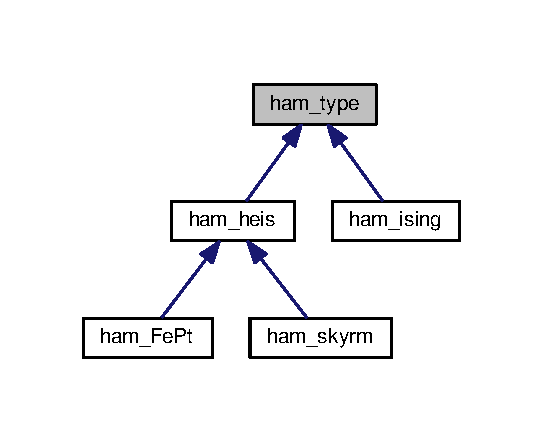
\includegraphics[width=261pt]{d5/d48/classham__type__inherit__graph}
\end{center}
\end{figure}
\subsection*{Public Member Functions}
\begin{DoxyCompactItemize}
\item 
virtual double \hyperlink{classham__type_a7fda5d3158544255ce3ca5e20c4e1c19}{calc\+\_\+E} (\hyperlink{classfield__type}{field\+\_\+type} $\ast$lattice)
\item 
virtual double \hyperlink{classham__type_a809902357229189b08ee9fdfab9c90be}{dE} (\hyperlink{classfield__type}{field\+\_\+type} $\ast$lattice, std\+::vector$<$ int $>$ \&position)
\item 
virtual std\+::vector$<$ double $>$ \hyperlink{classham__type_a953ba4332e88ee644d2afb96cd5a0ad5}{calc\+\_\+M} (\hyperlink{classfield__type}{field\+\_\+type} $\ast$lattice)
\item 
virtual std\+::vector$<$ double $>$ \hyperlink{classham__type_a37cc0a51074bd64cdeec866edb6f6015}{calc\+\_\+subM} (\hyperlink{classfield__type}{field\+\_\+type} $\ast$lattice, int subnumber)
\item 
virtual double \hyperlink{classham__type_ab75b9c6ea8098ea0874781a70bfa5099}{get\+\_\+J} () const 
\item 
virtual double \hyperlink{classham__type_a1c1a0ee7708f3d6f68bc999491dde42b}{get\+\_\+H} () const 
\item 
virtual std\+::vector$<$ double $>$ \hyperlink{classham__type_accdb77a4f5af92232a0415212d302344}{get\+\_\+\+Js} () const 
\item 
virtual std\+::vector$<$ double $>$ \hyperlink{classham__type_aab0cee1eece99ec37122126e7e4bcb91}{get\+\_\+\+Hs} () const 
\item 
virtual double \hyperlink{classham__type_a53ca8fb35d66cd07c78e24414b54d17f}{get\+\_\+K} () const 
\item 
virtual void \hyperlink{classham__type_a2864138405e794dc2aa2fe45fb6e400f}{get\+\_\+test} (double \&x, double \&y, double \&z)
\item 
virtual void \hyperlink{classham__type_a3a14214575bf8dcf3a8b39c7470dfe66}{init\+\_\+dim} (\hyperlink{classfield__type}{field\+\_\+type} $\ast$field)
\item 
virtual void \hyperlink{classham__type_a140c53e29c5c298c0f2704a4ecda7022}{set\+\_\+H} (double Hin)
\item 
virtual std\+::vector$<$ double $>$ \hyperlink{classham__type_ab6917097da83d4855efe2238ab4df4da}{calc\+\_\+top\+\_\+charge} (\hyperlink{classfield__type}{field\+\_\+type} $\ast$lattice)
\end{DoxyCompactItemize}
\subsection*{Protected Attributes}
\begin{DoxyCompactItemize}
\item 
int \hyperlink{classham__type_ae35098d4b40aee42316273b6cb439014}{dim}
\end{DoxyCompactItemize}


\subsection{Member Function Documentation}
\index{ham\+\_\+type@{ham\+\_\+type}!calc\+\_\+E@{calc\+\_\+E}}
\index{calc\+\_\+E@{calc\+\_\+E}!ham\+\_\+type@{ham\+\_\+type}}
\subsubsection[{\texorpdfstring{calc\+\_\+\+E(field\+\_\+type $\ast$lattice)}{calc_E(field_type *lattice)}}]{\setlength{\rightskip}{0pt plus 5cm}virtual double ham\+\_\+type\+::calc\+\_\+E (
\begin{DoxyParamCaption}
\item[{{\bf field\+\_\+type} $\ast$}]{lattice}
\end{DoxyParamCaption}
)\hspace{0.3cm}{\ttfamily [inline]}, {\ttfamily [virtual]}}\hypertarget{classham__type_a7fda5d3158544255ce3ca5e20c4e1c19}{}\label{classham__type_a7fda5d3158544255ce3ca5e20c4e1c19}


Reimplemented in \hyperlink{classham__skyrm_acca35df79a8fb4120efab41366564894}{ham\+\_\+skyrm}, \hyperlink{classham__FePt_a8d69322fbb999892889d34fb4b12f043}{ham\+\_\+\+Fe\+Pt}, \hyperlink{classham__heis_a9356396de229b2a0142fa6505f0132c1}{ham\+\_\+heis}, and \hyperlink{classham__ising_a04bdf2c223bada94ca813bc71d71e7cb}{ham\+\_\+ising}.

\index{ham\+\_\+type@{ham\+\_\+type}!calc\+\_\+M@{calc\+\_\+M}}
\index{calc\+\_\+M@{calc\+\_\+M}!ham\+\_\+type@{ham\+\_\+type}}
\subsubsection[{\texorpdfstring{calc\+\_\+\+M(field\+\_\+type $\ast$lattice)}{calc_M(field_type *lattice)}}]{\setlength{\rightskip}{0pt plus 5cm}virtual std\+::vector$<$double$>$ ham\+\_\+type\+::calc\+\_\+M (
\begin{DoxyParamCaption}
\item[{{\bf field\+\_\+type} $\ast$}]{lattice}
\end{DoxyParamCaption}
)\hspace{0.3cm}{\ttfamily [inline]}, {\ttfamily [virtual]}}\hypertarget{classham__type_a953ba4332e88ee644d2afb96cd5a0ad5}{}\label{classham__type_a953ba4332e88ee644d2afb96cd5a0ad5}


Reimplemented in \hyperlink{classham__heis_ab10e4c9b74e7182751715c670cf3c44c}{ham\+\_\+heis}, and \hyperlink{classham__ising_ad530e522cb6a2a80d10948603ff667ff}{ham\+\_\+ising}.

\index{ham\+\_\+type@{ham\+\_\+type}!calc\+\_\+subM@{calc\+\_\+subM}}
\index{calc\+\_\+subM@{calc\+\_\+subM}!ham\+\_\+type@{ham\+\_\+type}}
\subsubsection[{\texorpdfstring{calc\+\_\+sub\+M(field\+\_\+type $\ast$lattice, int subnumber)}{calc_subM(field_type *lattice, int subnumber)}}]{\setlength{\rightskip}{0pt plus 5cm}virtual std\+::vector$<$double$>$ ham\+\_\+type\+::calc\+\_\+subM (
\begin{DoxyParamCaption}
\item[{{\bf field\+\_\+type} $\ast$}]{lattice, }
\item[{int}]{subnumber}
\end{DoxyParamCaption}
)\hspace{0.3cm}{\ttfamily [inline]}, {\ttfamily [virtual]}}\hypertarget{classham__type_a37cc0a51074bd64cdeec866edb6f6015}{}\label{classham__type_a37cc0a51074bd64cdeec866edb6f6015}


Reimplemented in \hyperlink{classham__heis_a4713342c74601ac3246a34ebd429c07b}{ham\+\_\+heis}, and \hyperlink{classham__ising_a7092d807838fed1640bb03fa22e71236}{ham\+\_\+ising}.

\index{ham\+\_\+type@{ham\+\_\+type}!calc\+\_\+top\+\_\+charge@{calc\+\_\+top\+\_\+charge}}
\index{calc\+\_\+top\+\_\+charge@{calc\+\_\+top\+\_\+charge}!ham\+\_\+type@{ham\+\_\+type}}
\subsubsection[{\texorpdfstring{calc\+\_\+top\+\_\+charge(field\+\_\+type $\ast$lattice)}{calc_top_charge(field_type *lattice)}}]{\setlength{\rightskip}{0pt plus 5cm}virtual std\+::vector$<$double$>$ ham\+\_\+type\+::calc\+\_\+top\+\_\+charge (
\begin{DoxyParamCaption}
\item[{{\bf field\+\_\+type} $\ast$}]{lattice}
\end{DoxyParamCaption}
)\hspace{0.3cm}{\ttfamily [inline]}, {\ttfamily [virtual]}}\hypertarget{classham__type_ab6917097da83d4855efe2238ab4df4da}{}\label{classham__type_ab6917097da83d4855efe2238ab4df4da}


Reimplemented in \hyperlink{classham__heis_a12fedc92d02868a2eacfe2e3eb2578cf}{ham\+\_\+heis}.

\index{ham\+\_\+type@{ham\+\_\+type}!dE@{dE}}
\index{dE@{dE}!ham\+\_\+type@{ham\+\_\+type}}
\subsubsection[{\texorpdfstring{d\+E(field\+\_\+type $\ast$lattice, std\+::vector$<$ int $>$ \&position)}{dE(field_type *lattice, std::vector< int > &position)}}]{\setlength{\rightskip}{0pt plus 5cm}virtual double ham\+\_\+type\+::dE (
\begin{DoxyParamCaption}
\item[{{\bf field\+\_\+type} $\ast$}]{lattice, }
\item[{std\+::vector$<$ int $>$ \&}]{position}
\end{DoxyParamCaption}
)\hspace{0.3cm}{\ttfamily [inline]}, {\ttfamily [virtual]}}\hypertarget{classham__type_a809902357229189b08ee9fdfab9c90be}{}\label{classham__type_a809902357229189b08ee9fdfab9c90be}


Reimplemented in \hyperlink{classham__skyrm_aca80743449de874029fc0860fdd36422}{ham\+\_\+skyrm}, \hyperlink{classham__FePt_a742137dc8f3e289bb33abb3ad04d6a19}{ham\+\_\+\+Fe\+Pt}, \hyperlink{classham__heis_a80b17aefe298faa50b5cecb1aa9da4ad}{ham\+\_\+heis}, and \hyperlink{classham__ising_ae83e5c08a8da4652440ccd5d40554421}{ham\+\_\+ising}.

\index{ham\+\_\+type@{ham\+\_\+type}!get\+\_\+H@{get\+\_\+H}}
\index{get\+\_\+H@{get\+\_\+H}!ham\+\_\+type@{ham\+\_\+type}}
\subsubsection[{\texorpdfstring{get\+\_\+\+H() const }{get_H() const }}]{\setlength{\rightskip}{0pt plus 5cm}virtual double ham\+\_\+type\+::get\+\_\+H (
\begin{DoxyParamCaption}
{}
\end{DoxyParamCaption}
) const\hspace{0.3cm}{\ttfamily [inline]}, {\ttfamily [virtual]}}\hypertarget{classham__type_a1c1a0ee7708f3d6f68bc999491dde42b}{}\label{classham__type_a1c1a0ee7708f3d6f68bc999491dde42b}


Reimplemented in \hyperlink{classham__ising_aa03103158f5db829b8f17f43978a816c}{ham\+\_\+ising}.

\index{ham\+\_\+type@{ham\+\_\+type}!get\+\_\+\+Hs@{get\+\_\+\+Hs}}
\index{get\+\_\+\+Hs@{get\+\_\+\+Hs}!ham\+\_\+type@{ham\+\_\+type}}
\subsubsection[{\texorpdfstring{get\+\_\+\+Hs() const }{get_Hs() const }}]{\setlength{\rightskip}{0pt plus 5cm}virtual std\+::vector$<$double$>$ ham\+\_\+type\+::get\+\_\+\+Hs (
\begin{DoxyParamCaption}
{}
\end{DoxyParamCaption}
) const\hspace{0.3cm}{\ttfamily [inline]}, {\ttfamily [virtual]}}\hypertarget{classham__type_aab0cee1eece99ec37122126e7e4bcb91}{}\label{classham__type_aab0cee1eece99ec37122126e7e4bcb91}


Reimplemented in \hyperlink{classham__heis_afbdbe29a893440db2ddab8fd41775e56}{ham\+\_\+heis}.

\index{ham\+\_\+type@{ham\+\_\+type}!get\+\_\+J@{get\+\_\+J}}
\index{get\+\_\+J@{get\+\_\+J}!ham\+\_\+type@{ham\+\_\+type}}
\subsubsection[{\texorpdfstring{get\+\_\+\+J() const }{get_J() const }}]{\setlength{\rightskip}{0pt plus 5cm}virtual double ham\+\_\+type\+::get\+\_\+J (
\begin{DoxyParamCaption}
{}
\end{DoxyParamCaption}
) const\hspace{0.3cm}{\ttfamily [inline]}, {\ttfamily [virtual]}}\hypertarget{classham__type_ab75b9c6ea8098ea0874781a70bfa5099}{}\label{classham__type_ab75b9c6ea8098ea0874781a70bfa5099}


Reimplemented in \hyperlink{classham__ising_a3d5b100c6f3a1f750c524a2d302fd65e}{ham\+\_\+ising}.

\index{ham\+\_\+type@{ham\+\_\+type}!get\+\_\+\+Js@{get\+\_\+\+Js}}
\index{get\+\_\+\+Js@{get\+\_\+\+Js}!ham\+\_\+type@{ham\+\_\+type}}
\subsubsection[{\texorpdfstring{get\+\_\+\+Js() const }{get_Js() const }}]{\setlength{\rightskip}{0pt plus 5cm}virtual std\+::vector$<$double$>$ ham\+\_\+type\+::get\+\_\+\+Js (
\begin{DoxyParamCaption}
{}
\end{DoxyParamCaption}
) const\hspace{0.3cm}{\ttfamily [inline]}, {\ttfamily [virtual]}}\hypertarget{classham__type_accdb77a4f5af92232a0415212d302344}{}\label{classham__type_accdb77a4f5af92232a0415212d302344}


Reimplemented in \hyperlink{classham__heis_a177ac16e9cc6a7b2455c0271394362af}{ham\+\_\+heis}.

\index{ham\+\_\+type@{ham\+\_\+type}!get\+\_\+K@{get\+\_\+K}}
\index{get\+\_\+K@{get\+\_\+K}!ham\+\_\+type@{ham\+\_\+type}}
\subsubsection[{\texorpdfstring{get\+\_\+\+K() const }{get_K() const }}]{\setlength{\rightskip}{0pt plus 5cm}virtual double ham\+\_\+type\+::get\+\_\+K (
\begin{DoxyParamCaption}
{}
\end{DoxyParamCaption}
) const\hspace{0.3cm}{\ttfamily [inline]}, {\ttfamily [virtual]}}\hypertarget{classham__type_a53ca8fb35d66cd07c78e24414b54d17f}{}\label{classham__type_a53ca8fb35d66cd07c78e24414b54d17f}


Reimplemented in \hyperlink{classham__skyrm_a871473dff64abd906bed694a360335cf}{ham\+\_\+skyrm}.

\index{ham\+\_\+type@{ham\+\_\+type}!get\+\_\+test@{get\+\_\+test}}
\index{get\+\_\+test@{get\+\_\+test}!ham\+\_\+type@{ham\+\_\+type}}
\subsubsection[{\texorpdfstring{get\+\_\+test(double \&x, double \&y, double \&z)}{get_test(double &x, double &y, double &z)}}]{\setlength{\rightskip}{0pt plus 5cm}virtual void ham\+\_\+type\+::get\+\_\+test (
\begin{DoxyParamCaption}
\item[{double \&}]{x, }
\item[{double \&}]{y, }
\item[{double \&}]{z}
\end{DoxyParamCaption}
)\hspace{0.3cm}{\ttfamily [inline]}, {\ttfamily [virtual]}}\hypertarget{classham__type_a2864138405e794dc2aa2fe45fb6e400f}{}\label{classham__type_a2864138405e794dc2aa2fe45fb6e400f}


Reimplemented in \hyperlink{classham__heis_a3c603d70b56a9df357d3c39212395422}{ham\+\_\+heis}.

\index{ham\+\_\+type@{ham\+\_\+type}!init\+\_\+dim@{init\+\_\+dim}}
\index{init\+\_\+dim@{init\+\_\+dim}!ham\+\_\+type@{ham\+\_\+type}}
\subsubsection[{\texorpdfstring{init\+\_\+dim(field\+\_\+type $\ast$field)}{init_dim(field_type *field)}}]{\setlength{\rightskip}{0pt plus 5cm}virtual void ham\+\_\+type\+::init\+\_\+dim (
\begin{DoxyParamCaption}
\item[{{\bf field\+\_\+type} $\ast$}]{field}
\end{DoxyParamCaption}
)\hspace{0.3cm}{\ttfamily [inline]}, {\ttfamily [virtual]}}\hypertarget{classham__type_a3a14214575bf8dcf3a8b39c7470dfe66}{}\label{classham__type_a3a14214575bf8dcf3a8b39c7470dfe66}


Reimplemented in \hyperlink{classham__FePt_a3f03eee62cb90922ea4afea3fd1023e9}{ham\+\_\+\+Fe\+Pt}, \hyperlink{classham__heis_a48cfb1cf4cc50765d408113878f44979}{ham\+\_\+heis}, and \hyperlink{classham__ising_a92139385ee5cd3eab8a03897245dc53f}{ham\+\_\+ising}.

\index{ham\+\_\+type@{ham\+\_\+type}!set\+\_\+H@{set\+\_\+H}}
\index{set\+\_\+H@{set\+\_\+H}!ham\+\_\+type@{ham\+\_\+type}}
\subsubsection[{\texorpdfstring{set\+\_\+\+H(double Hin)}{set_H(double Hin)}}]{\setlength{\rightskip}{0pt plus 5cm}virtual void ham\+\_\+type\+::set\+\_\+H (
\begin{DoxyParamCaption}
\item[{double}]{Hin}
\end{DoxyParamCaption}
)\hspace{0.3cm}{\ttfamily [inline]}, {\ttfamily [virtual]}}\hypertarget{classham__type_a140c53e29c5c298c0f2704a4ecda7022}{}\label{classham__type_a140c53e29c5c298c0f2704a4ecda7022}


Reimplemented in \hyperlink{classham__heis_ab11ec994196743c909117b1231c6bfda}{ham\+\_\+heis}, and \hyperlink{classham__ising_a4b0bdb0e5576905061ec607cbeeb76cb}{ham\+\_\+ising}.



\subsection{Member Data Documentation}
\index{ham\+\_\+type@{ham\+\_\+type}!dim@{dim}}
\index{dim@{dim}!ham\+\_\+type@{ham\+\_\+type}}
\subsubsection[{\texorpdfstring{dim}{dim}}]{\setlength{\rightskip}{0pt plus 5cm}int ham\+\_\+type\+::dim\hspace{0.3cm}{\ttfamily [protected]}}\hypertarget{classham__type_ae35098d4b40aee42316273b6cb439014}{}\label{classham__type_ae35098d4b40aee42316273b6cb439014}


The documentation for this class was generated from the following file\+:\begin{DoxyCompactItemize}
\item 
includes/\hyperlink{hamiltonian_8hpp}{hamiltonian.\+hpp}\end{DoxyCompactItemize}

\hypertarget{classmklrand_1_1mkl__drand}{}\section{mklrand\+:\+:mkl\+\_\+drand Class Reference}
\label{classmklrand_1_1mkl__drand}\index{mklrand\+::mkl\+\_\+drand@{mklrand\+::mkl\+\_\+drand}}


Generator for uniform numbers between 0 and 1.  




{\ttfamily \#include $<$mklrand.\+hpp$>$}



Inheritance diagram for mklrand\+:\+:mkl\+\_\+drand\+:\nopagebreak
\begin{figure}[H]
\begin{center}
\leavevmode
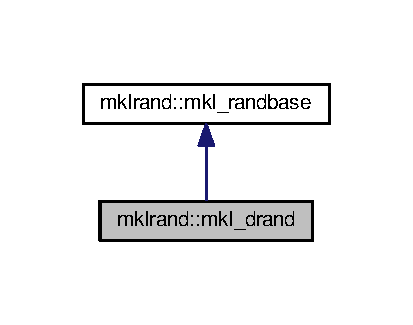
\includegraphics[width=198pt]{dd/de7/classmklrand_1_1mkl__drand__inherit__graph}
\end{center}
\end{figure}


Collaboration diagram for mklrand\+:\+:mkl\+\_\+drand\+:\nopagebreak
\begin{figure}[H]
\begin{center}
\leavevmode
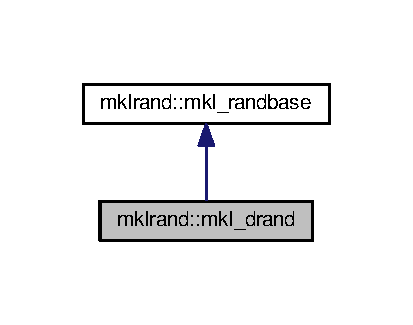
\includegraphics[width=198pt]{d7/d53/classmklrand_1_1mkl__drand__coll__graph}
\end{center}
\end{figure}
\subsection*{Public Member Functions}
\begin{DoxyCompactItemize}
\item 
\hyperlink{classmklrand_1_1mkl__drand_a2323c7fd79833d4e7920ec547625fe8b}{mkl\+\_\+drand} (int size, int seed=1)
\begin{DoxyCompactList}\small\item\em Constructor. \end{DoxyCompactList}\item 
\hyperlink{classmklrand_1_1mkl__drand_a4f6c0055cee5c0e5b9a82d95274bd0f5}{$\sim$mkl\+\_\+drand} ()
\begin{DoxyCompactList}\small\item\em Default destructor. \end{DoxyCompactList}\item 
double \hyperlink{classmklrand_1_1mkl__drand_a10d87b78fbb613e522b2429abf2c6097}{gen} ()
\begin{DoxyCompactList}\small\item\em Return a single random number. \end{DoxyCompactList}\item 
void \hyperlink{classmklrand_1_1mkl__drand_a085cf75b8a2330f2a3c368fff80ff478}{fill} ()
\begin{DoxyCompactList}\small\item\em Fill the buffer with new random numbers. \end{DoxyCompactList}\end{DoxyCompactItemize}
\subsection*{Additional Inherited Members}


\subsection{Detailed Description}
Generator for uniform numbers between 0 and 1. 

\subsection{Constructor \& Destructor Documentation}
\index{mklrand\+::mkl\+\_\+drand@{mklrand\+::mkl\+\_\+drand}!mkl\+\_\+drand@{mkl\+\_\+drand}}
\index{mkl\+\_\+drand@{mkl\+\_\+drand}!mklrand\+::mkl\+\_\+drand@{mklrand\+::mkl\+\_\+drand}}
\subsubsection[{\texorpdfstring{mkl\+\_\+drand(int size, int seed=1)}{mkl_drand(int size, int seed=1)}}]{\setlength{\rightskip}{0pt plus 5cm}mklrand\+::mkl\+\_\+drand\+::mkl\+\_\+drand (
\begin{DoxyParamCaption}
\item[{int}]{size, }
\item[{int}]{seed = {\ttfamily 1}}
\end{DoxyParamCaption}
)}\hypertarget{classmklrand_1_1mkl__drand_a2323c7fd79833d4e7920ec547625fe8b}{}\label{classmklrand_1_1mkl__drand_a2323c7fd79833d4e7920ec547625fe8b}


Constructor. 


\begin{DoxyParams}{Parameters}
{\em seed} & The inital seed of the random number generator. \\
\hline
{\em size} & The size of the buffer for R\+NG storage. \\
\hline
\end{DoxyParams}
\index{mklrand\+::mkl\+\_\+drand@{mklrand\+::mkl\+\_\+drand}!````~mkl\+\_\+drand@{$\sim$mkl\+\_\+drand}}
\index{````~mkl\+\_\+drand@{$\sim$mkl\+\_\+drand}!mklrand\+::mkl\+\_\+drand@{mklrand\+::mkl\+\_\+drand}}
\subsubsection[{\texorpdfstring{$\sim$mkl\+\_\+drand()}{~mkl_drand()}}]{\setlength{\rightskip}{0pt plus 5cm}mklrand\+::mkl\+\_\+drand\+::$\sim$mkl\+\_\+drand (
\begin{DoxyParamCaption}
{}
\end{DoxyParamCaption}
)}\hypertarget{classmklrand_1_1mkl__drand_a4f6c0055cee5c0e5b9a82d95274bd0f5}{}\label{classmklrand_1_1mkl__drand_a4f6c0055cee5c0e5b9a82d95274bd0f5}


Default destructor. 



\subsection{Member Function Documentation}
\index{mklrand\+::mkl\+\_\+drand@{mklrand\+::mkl\+\_\+drand}!fill@{fill}}
\index{fill@{fill}!mklrand\+::mkl\+\_\+drand@{mklrand\+::mkl\+\_\+drand}}
\subsubsection[{\texorpdfstring{fill()}{fill()}}]{\setlength{\rightskip}{0pt plus 5cm}void mklrand\+::mkl\+\_\+drand\+::fill (
\begin{DoxyParamCaption}
{}
\end{DoxyParamCaption}
)\hspace{0.3cm}{\ttfamily [virtual]}}\hypertarget{classmklrand_1_1mkl__drand_a085cf75b8a2330f2a3c368fff80ff478}{}\label{classmklrand_1_1mkl__drand_a085cf75b8a2330f2a3c368fff80ff478}


Fill the buffer with new random numbers. 



Reimplemented from \hyperlink{classmklrand_1_1mkl__randbase_ac00d006d5c8ad7eadc2e51f1b1604761}{mklrand\+::mkl\+\_\+randbase}.

\index{mklrand\+::mkl\+\_\+drand@{mklrand\+::mkl\+\_\+drand}!gen@{gen}}
\index{gen@{gen}!mklrand\+::mkl\+\_\+drand@{mklrand\+::mkl\+\_\+drand}}
\subsubsection[{\texorpdfstring{gen()}{gen()}}]{\setlength{\rightskip}{0pt plus 5cm}double mklrand\+::mkl\+\_\+drand\+::gen (
\begin{DoxyParamCaption}
{}
\end{DoxyParamCaption}
)}\hypertarget{classmklrand_1_1mkl__drand_a10d87b78fbb613e522b2429abf2c6097}{}\label{classmklrand_1_1mkl__drand_a10d87b78fbb613e522b2429abf2c6097}


Return a single random number. 



The documentation for this class was generated from the following file\+:\begin{DoxyCompactItemize}
\item 
includes/\hyperlink{mklrand_8hpp}{mklrand.\+hpp}\end{DoxyCompactItemize}

\hypertarget{classmklrand_1_1mkl__irand}{}\section{mklrand\+:\+:mkl\+\_\+irand Class Reference}
\label{classmklrand_1_1mkl__irand}\index{mklrand\+::mkl\+\_\+irand@{mklrand\+::mkl\+\_\+irand}}


Generator for uniform integers between 0 and 1.  




{\ttfamily \#include $<$mklrand.\+hpp$>$}



Inheritance diagram for mklrand\+:\+:mkl\+\_\+irand\+:
\nopagebreak
\begin{figure}[H]
\begin{center}
\leavevmode
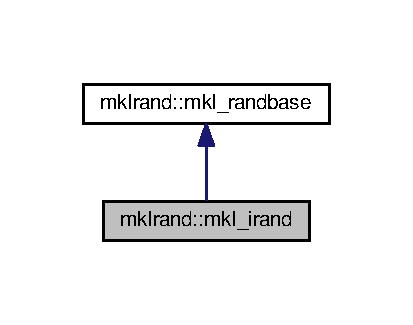
\includegraphics[width=198pt]{d0/d1e/classmklrand_1_1mkl__irand__inherit__graph}
\end{center}
\end{figure}


Collaboration diagram for mklrand\+:\+:mkl\+\_\+irand\+:
\nopagebreak
\begin{figure}[H]
\begin{center}
\leavevmode
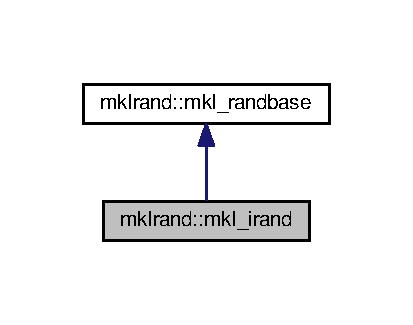
\includegraphics[width=198pt]{df/d22/classmklrand_1_1mkl__irand__coll__graph}
\end{center}
\end{figure}
\subsection*{Public Member Functions}
\begin{DoxyCompactItemize}
\item 
\hyperlink{classmklrand_1_1mkl__irand_a1f5cc9cb9269f9a24ee038aad3b64493}{mkl\+\_\+irand} (int size, int seed=1)
\begin{DoxyCompactList}\small\item\em Constructor. \end{DoxyCompactList}\item 
\hyperlink{classmklrand_1_1mkl__irand_a2febc3efc937b26f8cdb393a5f7735e5}{$\sim$mkl\+\_\+irand} ()
\begin{DoxyCompactList}\small\item\em Default destructor. \end{DoxyCompactList}\item 
int \hyperlink{classmklrand_1_1mkl__irand_a9e5b0289f101dc0ccd1aeff741714e5a}{gen} ()
\begin{DoxyCompactList}\small\item\em Return a single random number. \end{DoxyCompactList}\item 
void \hyperlink{classmklrand_1_1mkl__irand_ae1469013948288cef622ab879f56ff64}{fill} ()
\begin{DoxyCompactList}\small\item\em Fill the buffer with new random numbers. \end{DoxyCompactList}\end{DoxyCompactItemize}
\subsection*{Additional Inherited Members}


\subsection{Detailed Description}
Generator for uniform integers between 0 and 1. 

\subsection{Constructor \& Destructor Documentation}
\index{mklrand\+::mkl\+\_\+irand@{mklrand\+::mkl\+\_\+irand}!mkl\+\_\+irand@{mkl\+\_\+irand}}
\index{mkl\+\_\+irand@{mkl\+\_\+irand}!mklrand\+::mkl\+\_\+irand@{mklrand\+::mkl\+\_\+irand}}
\subsubsection[{\texorpdfstring{mkl\+\_\+irand(int size, int seed=1)}{mkl_irand(int size, int seed=1)}}]{\setlength{\rightskip}{0pt plus 5cm}mklrand\+::mkl\+\_\+irand\+::mkl\+\_\+irand (
\begin{DoxyParamCaption}
\item[{int}]{size, }
\item[{int}]{seed = {\ttfamily 1}}
\end{DoxyParamCaption}
)}\hypertarget{classmklrand_1_1mkl__irand_a1f5cc9cb9269f9a24ee038aad3b64493}{}\label{classmklrand_1_1mkl__irand_a1f5cc9cb9269f9a24ee038aad3b64493}


Constructor. 


\begin{DoxyParams}{Parameters}
{\em seed} & The inital seed of the random number generator. \\
\hline
{\em size} & The size of the buffer for R\+NG storage. \\
\hline
\end{DoxyParams}
\index{mklrand\+::mkl\+\_\+irand@{mklrand\+::mkl\+\_\+irand}!````~mkl\+\_\+irand@{$\sim$mkl\+\_\+irand}}
\index{````~mkl\+\_\+irand@{$\sim$mkl\+\_\+irand}!mklrand\+::mkl\+\_\+irand@{mklrand\+::mkl\+\_\+irand}}
\subsubsection[{\texorpdfstring{$\sim$mkl\+\_\+irand()}{~mkl_irand()}}]{\setlength{\rightskip}{0pt plus 5cm}mklrand\+::mkl\+\_\+irand\+::$\sim$mkl\+\_\+irand (
\begin{DoxyParamCaption}
{}
\end{DoxyParamCaption}
)}\hypertarget{classmklrand_1_1mkl__irand_a2febc3efc937b26f8cdb393a5f7735e5}{}\label{classmklrand_1_1mkl__irand_a2febc3efc937b26f8cdb393a5f7735e5}


Default destructor. 



\subsection{Member Function Documentation}
\index{mklrand\+::mkl\+\_\+irand@{mklrand\+::mkl\+\_\+irand}!fill@{fill}}
\index{fill@{fill}!mklrand\+::mkl\+\_\+irand@{mklrand\+::mkl\+\_\+irand}}
\subsubsection[{\texorpdfstring{fill()}{fill()}}]{\setlength{\rightskip}{0pt plus 5cm}void mklrand\+::mkl\+\_\+irand\+::fill (
\begin{DoxyParamCaption}
{}
\end{DoxyParamCaption}
)\hspace{0.3cm}{\ttfamily [virtual]}}\hypertarget{classmklrand_1_1mkl__irand_ae1469013948288cef622ab879f56ff64}{}\label{classmklrand_1_1mkl__irand_ae1469013948288cef622ab879f56ff64}


Fill the buffer with new random numbers. 



Reimplemented from \hyperlink{classmklrand_1_1mkl__randbase_ac00d006d5c8ad7eadc2e51f1b1604761}{mklrand\+::mkl\+\_\+randbase}.

\index{mklrand\+::mkl\+\_\+irand@{mklrand\+::mkl\+\_\+irand}!gen@{gen}}
\index{gen@{gen}!mklrand\+::mkl\+\_\+irand@{mklrand\+::mkl\+\_\+irand}}
\subsubsection[{\texorpdfstring{gen()}{gen()}}]{\setlength{\rightskip}{0pt plus 5cm}int mklrand\+::mkl\+\_\+irand\+::gen (
\begin{DoxyParamCaption}
{}
\end{DoxyParamCaption}
)}\hypertarget{classmklrand_1_1mkl__irand_a9e5b0289f101dc0ccd1aeff741714e5a}{}\label{classmklrand_1_1mkl__irand_a9e5b0289f101dc0ccd1aeff741714e5a}


Return a single random number. 



The documentation for this class was generated from the following file\+:\begin{DoxyCompactItemize}
\item 
includes/\hyperlink{mklrand_8hpp}{mklrand.\+hpp}\end{DoxyCompactItemize}

\hypertarget{classmklrand_1_1mkl__lnrand}{}\section{mklrand\+:\+:mkl\+\_\+lnrand Class Reference}
\label{classmklrand_1_1mkl__lnrand}\index{mklrand\+::mkl\+\_\+lnrand@{mklrand\+::mkl\+\_\+lnrand}}


Generator for random numbers on a lognormal distribution.  




{\ttfamily \#include $<$mklrand.\+hpp$>$}



Inheritance diagram for mklrand\+:\+:mkl\+\_\+lnrand\+:\nopagebreak
\begin{figure}[H]
\begin{center}
\leavevmode
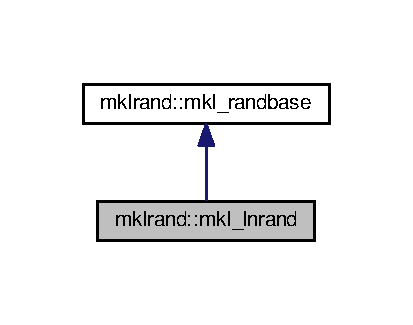
\includegraphics[width=198pt]{d0/d84/classmklrand_1_1mkl__lnrand__inherit__graph}
\end{center}
\end{figure}


Collaboration diagram for mklrand\+:\+:mkl\+\_\+lnrand\+:\nopagebreak
\begin{figure}[H]
\begin{center}
\leavevmode
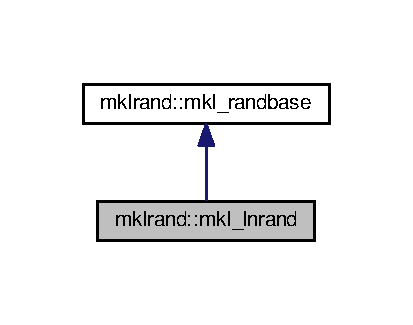
\includegraphics[width=198pt]{da/dc6/classmklrand_1_1mkl__lnrand__coll__graph}
\end{center}
\end{figure}
\subsection*{Public Member Functions}
\begin{DoxyCompactItemize}
\item 
\hyperlink{classmklrand_1_1mkl__lnrand_a39faf5aa38fae7ac1ef6e3f473ccf8a2}{mkl\+\_\+lnrand} (double m, double sd, int size, int seed=1)
\begin{DoxyCompactList}\small\item\em Constructor. \end{DoxyCompactList}\item 
\hyperlink{classmklrand_1_1mkl__lnrand_adb4d71f9ee8992fa1e595af7ec7005c3}{$\sim$mkl\+\_\+lnrand} ()
\begin{DoxyCompactList}\small\item\em Default destructor. \end{DoxyCompactList}\item 
double \hyperlink{classmklrand_1_1mkl__lnrand_a3eba34d1b1f2f448a782eb06a03459e5}{gen} ()
\begin{DoxyCompactList}\small\item\em Return a single random number. \end{DoxyCompactList}\item 
void \hyperlink{classmklrand_1_1mkl__lnrand_ac43f4c40429885f5306dce10adf5d04a}{fill} ()
\begin{DoxyCompactList}\small\item\em Fill the buffer with new random numbers. \end{DoxyCompactList}\end{DoxyCompactItemize}
\subsection*{Additional Inherited Members}


\subsection{Detailed Description}
Generator for random numbers on a lognormal distribution. 

\subsection{Constructor \& Destructor Documentation}
\index{mklrand\+::mkl\+\_\+lnrand@{mklrand\+::mkl\+\_\+lnrand}!mkl\+\_\+lnrand@{mkl\+\_\+lnrand}}
\index{mkl\+\_\+lnrand@{mkl\+\_\+lnrand}!mklrand\+::mkl\+\_\+lnrand@{mklrand\+::mkl\+\_\+lnrand}}
\subsubsection[{\texorpdfstring{mkl\+\_\+lnrand(double m, double sd, int size, int seed=1)}{mkl_lnrand(double m, double sd, int size, int seed=1)}}]{\setlength{\rightskip}{0pt plus 5cm}mklrand\+::mkl\+\_\+lnrand\+::mkl\+\_\+lnrand (
\begin{DoxyParamCaption}
\item[{double}]{m, }
\item[{double}]{sd, }
\item[{int}]{size, }
\item[{int}]{seed = {\ttfamily 1}}
\end{DoxyParamCaption}
)}\hypertarget{classmklrand_1_1mkl__lnrand_a39faf5aa38fae7ac1ef6e3f473ccf8a2}{}\label{classmklrand_1_1mkl__lnrand_a39faf5aa38fae7ac1ef6e3f473ccf8a2}


Constructor. 


\begin{DoxyParams}{Parameters}
{\em seed} & The inital seed of the random number generator. \\
\hline
{\em size} & The size of the buffer for R\+NG storage. \\
\hline
{\em m} & The logarithmic mean of the distribution. \\
\hline
{\em sd} & The logarithmic standard devaiation of the distribution. \\
\hline
\end{DoxyParams}
\index{mklrand\+::mkl\+\_\+lnrand@{mklrand\+::mkl\+\_\+lnrand}!````~mkl\+\_\+lnrand@{$\sim$mkl\+\_\+lnrand}}
\index{````~mkl\+\_\+lnrand@{$\sim$mkl\+\_\+lnrand}!mklrand\+::mkl\+\_\+lnrand@{mklrand\+::mkl\+\_\+lnrand}}
\subsubsection[{\texorpdfstring{$\sim$mkl\+\_\+lnrand()}{~mkl_lnrand()}}]{\setlength{\rightskip}{0pt plus 5cm}mklrand\+::mkl\+\_\+lnrand\+::$\sim$mkl\+\_\+lnrand (
\begin{DoxyParamCaption}
{}
\end{DoxyParamCaption}
)}\hypertarget{classmklrand_1_1mkl__lnrand_adb4d71f9ee8992fa1e595af7ec7005c3}{}\label{classmklrand_1_1mkl__lnrand_adb4d71f9ee8992fa1e595af7ec7005c3}


Default destructor. 



\subsection{Member Function Documentation}
\index{mklrand\+::mkl\+\_\+lnrand@{mklrand\+::mkl\+\_\+lnrand}!fill@{fill}}
\index{fill@{fill}!mklrand\+::mkl\+\_\+lnrand@{mklrand\+::mkl\+\_\+lnrand}}
\subsubsection[{\texorpdfstring{fill()}{fill()}}]{\setlength{\rightskip}{0pt plus 5cm}void mklrand\+::mkl\+\_\+lnrand\+::fill (
\begin{DoxyParamCaption}
{}
\end{DoxyParamCaption}
)\hspace{0.3cm}{\ttfamily [virtual]}}\hypertarget{classmklrand_1_1mkl__lnrand_ac43f4c40429885f5306dce10adf5d04a}{}\label{classmklrand_1_1mkl__lnrand_ac43f4c40429885f5306dce10adf5d04a}


Fill the buffer with new random numbers. 



Reimplemented from \hyperlink{classmklrand_1_1mkl__randbase_ac00d006d5c8ad7eadc2e51f1b1604761}{mklrand\+::mkl\+\_\+randbase}.

\index{mklrand\+::mkl\+\_\+lnrand@{mklrand\+::mkl\+\_\+lnrand}!gen@{gen}}
\index{gen@{gen}!mklrand\+::mkl\+\_\+lnrand@{mklrand\+::mkl\+\_\+lnrand}}
\subsubsection[{\texorpdfstring{gen()}{gen()}}]{\setlength{\rightskip}{0pt plus 5cm}double mklrand\+::mkl\+\_\+lnrand\+::gen (
\begin{DoxyParamCaption}
{}
\end{DoxyParamCaption}
)}\hypertarget{classmklrand_1_1mkl__lnrand_a3eba34d1b1f2f448a782eb06a03459e5}{}\label{classmklrand_1_1mkl__lnrand_a3eba34d1b1f2f448a782eb06a03459e5}


Return a single random number. 



The documentation for this class was generated from the following file\+:\begin{DoxyCompactItemize}
\item 
includes/\hyperlink{mklrand_8hpp}{mklrand.\+hpp}\end{DoxyCompactItemize}

\hypertarget{classmklrand_1_1mkl__randbase}{}\section{mklrand\+:\+:mkl\+\_\+randbase Class Reference}
\label{classmklrand_1_1mkl__randbase}\index{mklrand\+::mkl\+\_\+randbase@{mklrand\+::mkl\+\_\+randbase}}


Base class for the random number generators.  




{\ttfamily \#include $<$mklrand.\+hpp$>$}



Inheritance diagram for mklrand\+:\+:mkl\+\_\+randbase\+:
\nopagebreak
\begin{figure}[H]
\begin{center}
\leavevmode
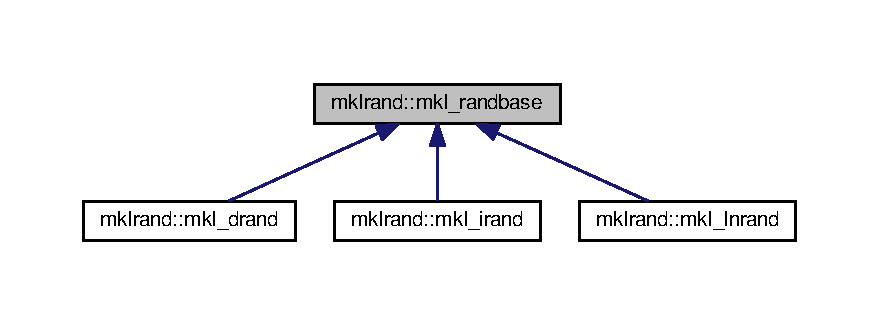
\includegraphics[width=350pt]{db/d0e/classmklrand_1_1mkl__randbase__inherit__graph}
\end{center}
\end{figure}
\subsection*{Public Member Functions}
\begin{DoxyCompactItemize}
\item 
\hyperlink{classmklrand_1_1mkl__randbase_a83f8b1954a948117ae433d93ff986ff0}{mkl\+\_\+randbase} ()
\begin{DoxyCompactList}\small\item\em Default constructor. \end{DoxyCompactList}\item 
\hyperlink{classmklrand_1_1mkl__randbase_a696e5a448c313959a55d21a02193a745}{$\sim$mkl\+\_\+randbase} ()
\begin{DoxyCompactList}\small\item\em Default destructor. \end{DoxyCompactList}\item 
virtual void \hyperlink{classmklrand_1_1mkl__randbase_ac00d006d5c8ad7eadc2e51f1b1604761}{fill} ()
\begin{DoxyCompactList}\small\item\em Fill the buffer with new random numbers. \end{DoxyCompactList}\item 
void \hyperlink{classmklrand_1_1mkl__randbase_a4f41864ffa41b49f69cbac7934edda3e}{change\+\_\+seed} (int seed)
\begin{DoxyCompactList}\small\item\em Change the current random seed. \end{DoxyCompactList}\item 
void \hyperlink{classmklrand_1_1mkl__randbase_a86c4b056e414a635cc12f6530f74f30c}{save} (const char $\ast$name)
\begin{DoxyCompactList}\small\item\em Save the state of the random number generator. \end{DoxyCompactList}\item 
void \hyperlink{classmklrand_1_1mkl__randbase_a37e1bfcc4835e09301d9bac95a446f20}{load} (const char $\ast$name)
\begin{DoxyCompactList}\small\item\em Load a random number generator state. \end{DoxyCompactList}\end{DoxyCompactItemize}
\subsection*{Protected Attributes}
\begin{DoxyCompactItemize}
\item 
int \hyperlink{classmklrand_1_1mkl__randbase_a1e090cd68b19d7d05b4e3f32e5c7a171}{arr\+\_\+size}
\item 
int \hyperlink{classmklrand_1_1mkl__randbase_aeb5c3f18b6d46a6ee53cfeb2a1d95388}{curr}
\item 
V\+S\+L\+Stream\+State\+Ptr \hyperlink{classmklrand_1_1mkl__randbase_a1668b51838583d64b176e159b16bfa7a}{stream}
\end{DoxyCompactItemize}


\subsection{Detailed Description}
Base class for the random number generators. 

\subsection{Constructor \& Destructor Documentation}
\index{mklrand\+::mkl\+\_\+randbase@{mklrand\+::mkl\+\_\+randbase}!mkl\+\_\+randbase@{mkl\+\_\+randbase}}
\index{mkl\+\_\+randbase@{mkl\+\_\+randbase}!mklrand\+::mkl\+\_\+randbase@{mklrand\+::mkl\+\_\+randbase}}
\subsubsection[{\texorpdfstring{mkl\+\_\+randbase()}{mkl_randbase()}}]{\setlength{\rightskip}{0pt plus 5cm}mklrand\+::mkl\+\_\+randbase\+::mkl\+\_\+randbase (
\begin{DoxyParamCaption}
{}
\end{DoxyParamCaption}
)\hspace{0.3cm}{\ttfamily [inline]}}\hypertarget{classmklrand_1_1mkl__randbase_a83f8b1954a948117ae433d93ff986ff0}{}\label{classmklrand_1_1mkl__randbase_a83f8b1954a948117ae433d93ff986ff0}


Default constructor. 

\index{mklrand\+::mkl\+\_\+randbase@{mklrand\+::mkl\+\_\+randbase}!````~mkl\+\_\+randbase@{$\sim$mkl\+\_\+randbase}}
\index{````~mkl\+\_\+randbase@{$\sim$mkl\+\_\+randbase}!mklrand\+::mkl\+\_\+randbase@{mklrand\+::mkl\+\_\+randbase}}
\subsubsection[{\texorpdfstring{$\sim$mkl\+\_\+randbase()}{~mkl_randbase()}}]{\setlength{\rightskip}{0pt plus 5cm}mklrand\+::mkl\+\_\+randbase\+::$\sim$mkl\+\_\+randbase (
\begin{DoxyParamCaption}
{}
\end{DoxyParamCaption}
)\hspace{0.3cm}{\ttfamily [inline]}}\hypertarget{classmklrand_1_1mkl__randbase_a696e5a448c313959a55d21a02193a745}{}\label{classmklrand_1_1mkl__randbase_a696e5a448c313959a55d21a02193a745}


Default destructor. 



\subsection{Member Function Documentation}
\index{mklrand\+::mkl\+\_\+randbase@{mklrand\+::mkl\+\_\+randbase}!change\+\_\+seed@{change\+\_\+seed}}
\index{change\+\_\+seed@{change\+\_\+seed}!mklrand\+::mkl\+\_\+randbase@{mklrand\+::mkl\+\_\+randbase}}
\subsubsection[{\texorpdfstring{change\+\_\+seed(int seed)}{change_seed(int seed)}}]{\setlength{\rightskip}{0pt plus 5cm}void mklrand\+::mkl\+\_\+randbase\+::change\+\_\+seed (
\begin{DoxyParamCaption}
\item[{int}]{seed}
\end{DoxyParamCaption}
)}\hypertarget{classmklrand_1_1mkl__randbase_a4f41864ffa41b49f69cbac7934edda3e}{}\label{classmklrand_1_1mkl__randbase_a4f41864ffa41b49f69cbac7934edda3e}


Change the current random seed. 


\begin{DoxyParams}{Parameters}
{\em seed} & The new seed. \\
\hline
\end{DoxyParams}
\index{mklrand\+::mkl\+\_\+randbase@{mklrand\+::mkl\+\_\+randbase}!fill@{fill}}
\index{fill@{fill}!mklrand\+::mkl\+\_\+randbase@{mklrand\+::mkl\+\_\+randbase}}
\subsubsection[{\texorpdfstring{fill()}{fill()}}]{\setlength{\rightskip}{0pt plus 5cm}virtual void mklrand\+::mkl\+\_\+randbase\+::fill (
\begin{DoxyParamCaption}
{}
\end{DoxyParamCaption}
)\hspace{0.3cm}{\ttfamily [inline]}, {\ttfamily [virtual]}}\hypertarget{classmklrand_1_1mkl__randbase_ac00d006d5c8ad7eadc2e51f1b1604761}{}\label{classmklrand_1_1mkl__randbase_ac00d006d5c8ad7eadc2e51f1b1604761}


Fill the buffer with new random numbers. 



Reimplemented in \hyperlink{classmklrand_1_1mkl__lnrand_ac43f4c40429885f5306dce10adf5d04a}{mklrand\+::mkl\+\_\+lnrand}, \hyperlink{classmklrand_1_1mkl__irand_ae1469013948288cef622ab879f56ff64}{mklrand\+::mkl\+\_\+irand}, and \hyperlink{classmklrand_1_1mkl__drand_a085cf75b8a2330f2a3c368fff80ff478}{mklrand\+::mkl\+\_\+drand}.

\index{mklrand\+::mkl\+\_\+randbase@{mklrand\+::mkl\+\_\+randbase}!load@{load}}
\index{load@{load}!mklrand\+::mkl\+\_\+randbase@{mklrand\+::mkl\+\_\+randbase}}
\subsubsection[{\texorpdfstring{load(const char $\ast$name)}{load(const char *name)}}]{\setlength{\rightskip}{0pt plus 5cm}void mklrand\+::mkl\+\_\+randbase\+::load (
\begin{DoxyParamCaption}
\item[{const char $\ast$}]{name}
\end{DoxyParamCaption}
)\hspace{0.3cm}{\ttfamily [inline]}}\hypertarget{classmklrand_1_1mkl__randbase_a37e1bfcc4835e09301d9bac95a446f20}{}\label{classmklrand_1_1mkl__randbase_a37e1bfcc4835e09301d9bac95a446f20}


Load a random number generator state. 


\begin{DoxyParams}{Parameters}
{\em name} & The name of the file which the state loaded from. \\
\hline
\end{DoxyParams}
\index{mklrand\+::mkl\+\_\+randbase@{mklrand\+::mkl\+\_\+randbase}!save@{save}}
\index{save@{save}!mklrand\+::mkl\+\_\+randbase@{mklrand\+::mkl\+\_\+randbase}}
\subsubsection[{\texorpdfstring{save(const char $\ast$name)}{save(const char *name)}}]{\setlength{\rightskip}{0pt plus 5cm}void mklrand\+::mkl\+\_\+randbase\+::save (
\begin{DoxyParamCaption}
\item[{const char $\ast$}]{name}
\end{DoxyParamCaption}
)\hspace{0.3cm}{\ttfamily [inline]}}\hypertarget{classmklrand_1_1mkl__randbase_a86c4b056e414a635cc12f6530f74f30c}{}\label{classmklrand_1_1mkl__randbase_a86c4b056e414a635cc12f6530f74f30c}


Save the state of the random number generator. 


\begin{DoxyParams}{Parameters}
{\em name} & The name of the file which the state will be saved to. \\
\hline
\end{DoxyParams}


\subsection{Member Data Documentation}
\index{mklrand\+::mkl\+\_\+randbase@{mklrand\+::mkl\+\_\+randbase}!arr\+\_\+size@{arr\+\_\+size}}
\index{arr\+\_\+size@{arr\+\_\+size}!mklrand\+::mkl\+\_\+randbase@{mklrand\+::mkl\+\_\+randbase}}
\subsubsection[{\texorpdfstring{arr\+\_\+size}{arr_size}}]{\setlength{\rightskip}{0pt plus 5cm}int mklrand\+::mkl\+\_\+randbase\+::arr\+\_\+size\hspace{0.3cm}{\ttfamily [protected]}}\hypertarget{classmklrand_1_1mkl__randbase_a1e090cd68b19d7d05b4e3f32e5c7a171}{}\label{classmklrand_1_1mkl__randbase_a1e090cd68b19d7d05b4e3f32e5c7a171}
\index{mklrand\+::mkl\+\_\+randbase@{mklrand\+::mkl\+\_\+randbase}!curr@{curr}}
\index{curr@{curr}!mklrand\+::mkl\+\_\+randbase@{mklrand\+::mkl\+\_\+randbase}}
\subsubsection[{\texorpdfstring{curr}{curr}}]{\setlength{\rightskip}{0pt plus 5cm}int mklrand\+::mkl\+\_\+randbase\+::curr\hspace{0.3cm}{\ttfamily [protected]}}\hypertarget{classmklrand_1_1mkl__randbase_aeb5c3f18b6d46a6ee53cfeb2a1d95388}{}\label{classmklrand_1_1mkl__randbase_aeb5c3f18b6d46a6ee53cfeb2a1d95388}
\index{mklrand\+::mkl\+\_\+randbase@{mklrand\+::mkl\+\_\+randbase}!stream@{stream}}
\index{stream@{stream}!mklrand\+::mkl\+\_\+randbase@{mklrand\+::mkl\+\_\+randbase}}
\subsubsection[{\texorpdfstring{stream}{stream}}]{\setlength{\rightskip}{0pt plus 5cm}V\+S\+L\+Stream\+State\+Ptr mklrand\+::mkl\+\_\+randbase\+::stream\hspace{0.3cm}{\ttfamily [protected]}}\hypertarget{classmklrand_1_1mkl__randbase_a1668b51838583d64b176e159b16bfa7a}{}\label{classmklrand_1_1mkl__randbase_a1668b51838583d64b176e159b16bfa7a}


The documentation for this class was generated from the following file\+:\begin{DoxyCompactItemize}
\item 
includes/\hyperlink{mklrand_8hpp}{mklrand.\+hpp}\end{DoxyCompactItemize}

\hypertarget{classparticle_1_1shape_1_1sh__cluster}{}\section{particle\+:\+:shape\+:\+:sh\+\_\+cluster Class Reference}
\label{classparticle_1_1shape_1_1sh__cluster}\index{particle\+::shape\+::sh\+\_\+cluster@{particle\+::shape\+::sh\+\_\+cluster}}


Particle cluster (depreciated)  




{\ttfamily \#include $<$shape.\+hpp$>$}



Inheritance diagram for particle\+:\+:shape\+:\+:sh\+\_\+cluster\+:\nopagebreak
\begin{figure}[H]
\begin{center}
\leavevmode
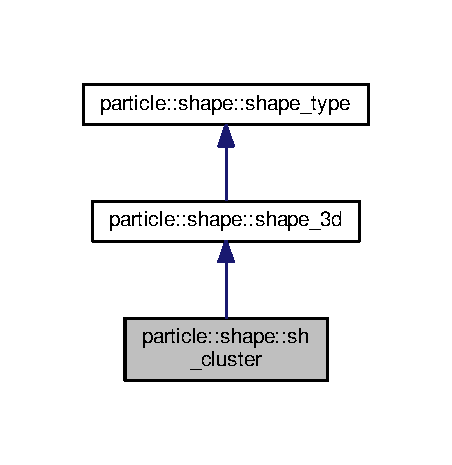
\includegraphics[width=217pt]{d8/d55/classparticle_1_1shape_1_1sh__cluster__inherit__graph}
\end{center}
\end{figure}


Collaboration diagram for particle\+:\+:shape\+:\+:sh\+\_\+cluster\+:\nopagebreak
\begin{figure}[H]
\begin{center}
\leavevmode
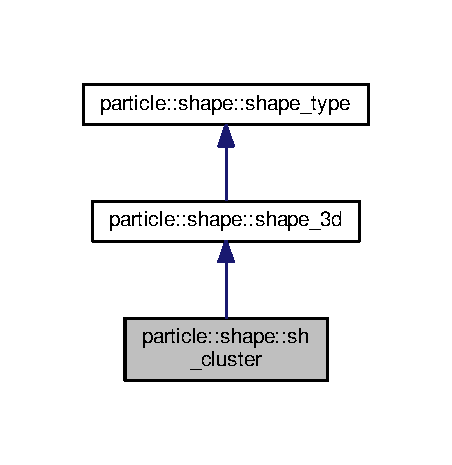
\includegraphics[width=217pt]{d6/d9e/classparticle_1_1shape_1_1sh__cluster__coll__graph}
\end{center}
\end{figure}
\subsection*{Public Member Functions}
\begin{DoxyCompactItemize}
\item 
\hyperlink{classparticle_1_1shape_1_1sh__cluster_a35768f3d2687ff2f178d465866fbb837}{sh\+\_\+cluster} ()
\begin{DoxyCompactList}\small\item\em Default constructor. \end{DoxyCompactList}\item 
\hyperlink{classparticle_1_1shape_1_1sh__cluster_acbb95a92e18fca21853a06c3c6d56524}{$\sim$sh\+\_\+cluster} ()
\begin{DoxyCompactList}\small\item\em Default destructor. \end{DoxyCompactList}\end{DoxyCompactItemize}


\subsection{Detailed Description}
Particle cluster (depreciated) 

\subsection{Constructor \& Destructor Documentation}
\index{particle\+::shape\+::sh\+\_\+cluster@{particle\+::shape\+::sh\+\_\+cluster}!sh\+\_\+cluster@{sh\+\_\+cluster}}
\index{sh\+\_\+cluster@{sh\+\_\+cluster}!particle\+::shape\+::sh\+\_\+cluster@{particle\+::shape\+::sh\+\_\+cluster}}
\subsubsection[{\texorpdfstring{sh\+\_\+cluster()}{sh_cluster()}}]{\setlength{\rightskip}{0pt plus 5cm}particle\+::shape\+::sh\+\_\+cluster\+::sh\+\_\+cluster (
\begin{DoxyParamCaption}
{}
\end{DoxyParamCaption}
)\hspace{0.3cm}{\ttfamily [inline]}}\hypertarget{classparticle_1_1shape_1_1sh__cluster_a35768f3d2687ff2f178d465866fbb837}{}\label{classparticle_1_1shape_1_1sh__cluster_a35768f3d2687ff2f178d465866fbb837}


Default constructor. 

\index{particle\+::shape\+::sh\+\_\+cluster@{particle\+::shape\+::sh\+\_\+cluster}!````~sh\+\_\+cluster@{$\sim$sh\+\_\+cluster}}
\index{````~sh\+\_\+cluster@{$\sim$sh\+\_\+cluster}!particle\+::shape\+::sh\+\_\+cluster@{particle\+::shape\+::sh\+\_\+cluster}}
\subsubsection[{\texorpdfstring{$\sim$sh\+\_\+cluster()}{~sh_cluster()}}]{\setlength{\rightskip}{0pt plus 5cm}particle\+::shape\+::sh\+\_\+cluster\+::$\sim$sh\+\_\+cluster (
\begin{DoxyParamCaption}
{}
\end{DoxyParamCaption}
)\hspace{0.3cm}{\ttfamily [inline]}}\hypertarget{classparticle_1_1shape_1_1sh__cluster_acbb95a92e18fca21853a06c3c6d56524}{}\label{classparticle_1_1shape_1_1sh__cluster_acbb95a92e18fca21853a06c3c6d56524}


Default destructor. 



The documentation for this class was generated from the following file\+:\begin{DoxyCompactItemize}
\item 
includes/\hyperlink{shape_8hpp}{shape.\+hpp}\end{DoxyCompactItemize}

\hypertarget{classparticle_1_1shape_1_1shape__2d}{}\section{particle\+:\+:shape\+:\+:shape\+\_\+2d Class Reference}
\label{classparticle_1_1shape_1_1shape__2d}\index{particle\+::shape\+::shape\+\_\+2d@{particle\+::shape\+::shape\+\_\+2d}}


2D particle shapes.  




{\ttfamily \#include $<$shape.\+hpp$>$}



Inheritance diagram for particle\+:\+:shape\+:\+:shape\+\_\+2d\+:\nopagebreak
\begin{figure}[H]
\begin{center}
\leavevmode
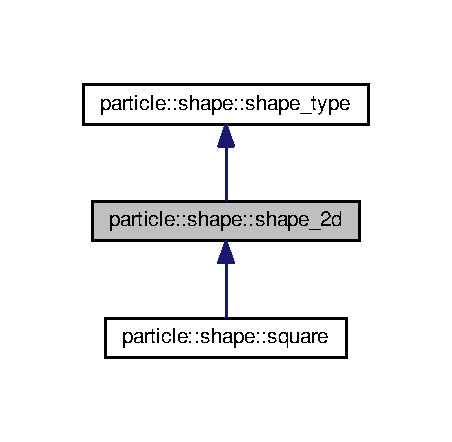
\includegraphics[width=217pt]{db/d00/classparticle_1_1shape_1_1shape__2d__inherit__graph}
\end{center}
\end{figure}


Collaboration diagram for particle\+:\+:shape\+:\+:shape\+\_\+2d\+:\nopagebreak
\begin{figure}[H]
\begin{center}
\leavevmode
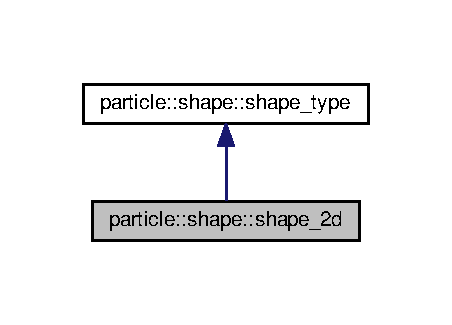
\includegraphics[width=217pt]{df/df8/classparticle_1_1shape_1_1shape__2d__coll__graph}
\end{center}
\end{figure}
\subsection*{Public Member Functions}
\begin{DoxyCompactItemize}
\item 
\hyperlink{classparticle_1_1shape_1_1shape__2d_a72d23ad24e5a3acc3948fbceb44591a4}{shape\+\_\+2d} ()
\begin{DoxyCompactList}\small\item\em Default constructor. \end{DoxyCompactList}\item 
\hyperlink{classparticle_1_1shape_1_1shape__2d_a6ea97cd4eedece84d77c9faa4fc960d2}{$\sim$shape\+\_\+2d} ()
\begin{DoxyCompactList}\small\item\em Default destructor. \end{DoxyCompactList}\item 
virtual bool \hyperlink{classparticle_1_1shape_1_1shape__2d_a756e06b46afd0e18d6a37a0a8f28551c}{check} (std\+::vector$<$ int $>$ Is, int l\+\_\+size)
\begin{DoxyCompactList}\small\item\em Check whether a certain position falls within the particle. \end{DoxyCompactList}\end{DoxyCompactItemize}


\subsection{Detailed Description}
2D particle shapes. 

\subsection{Constructor \& Destructor Documentation}
\index{particle\+::shape\+::shape\+\_\+2d@{particle\+::shape\+::shape\+\_\+2d}!shape\+\_\+2d@{shape\+\_\+2d}}
\index{shape\+\_\+2d@{shape\+\_\+2d}!particle\+::shape\+::shape\+\_\+2d@{particle\+::shape\+::shape\+\_\+2d}}
\subsubsection[{\texorpdfstring{shape\+\_\+2d()}{shape_2d()}}]{\setlength{\rightskip}{0pt plus 5cm}particle\+::shape\+::shape\+\_\+2d\+::shape\+\_\+2d (
\begin{DoxyParamCaption}
{}
\end{DoxyParamCaption}
)\hspace{0.3cm}{\ttfamily [inline]}}\hypertarget{classparticle_1_1shape_1_1shape__2d_a72d23ad24e5a3acc3948fbceb44591a4}{}\label{classparticle_1_1shape_1_1shape__2d_a72d23ad24e5a3acc3948fbceb44591a4}


Default constructor. 

\index{particle\+::shape\+::shape\+\_\+2d@{particle\+::shape\+::shape\+\_\+2d}!````~shape\+\_\+2d@{$\sim$shape\+\_\+2d}}
\index{````~shape\+\_\+2d@{$\sim$shape\+\_\+2d}!particle\+::shape\+::shape\+\_\+2d@{particle\+::shape\+::shape\+\_\+2d}}
\subsubsection[{\texorpdfstring{$\sim$shape\+\_\+2d()}{~shape_2d()}}]{\setlength{\rightskip}{0pt plus 5cm}particle\+::shape\+::shape\+\_\+2d\+::$\sim$shape\+\_\+2d (
\begin{DoxyParamCaption}
{}
\end{DoxyParamCaption}
)\hspace{0.3cm}{\ttfamily [inline]}}\hypertarget{classparticle_1_1shape_1_1shape__2d_a6ea97cd4eedece84d77c9faa4fc960d2}{}\label{classparticle_1_1shape_1_1shape__2d_a6ea97cd4eedece84d77c9faa4fc960d2}


Default destructor. 



\subsection{Member Function Documentation}
\index{particle\+::shape\+::shape\+\_\+2d@{particle\+::shape\+::shape\+\_\+2d}!check@{check}}
\index{check@{check}!particle\+::shape\+::shape\+\_\+2d@{particle\+::shape\+::shape\+\_\+2d}}
\subsubsection[{\texorpdfstring{check(std\+::vector$<$ int $>$ Is, int l\+\_\+size)}{check(std::vector< int > Is, int l_size)}}]{\setlength{\rightskip}{0pt plus 5cm}virtual bool particle\+::shape\+::shape\+\_\+2d\+::check (
\begin{DoxyParamCaption}
\item[{std\+::vector$<$ int $>$}]{Is, }
\item[{int}]{l\+\_\+size}
\end{DoxyParamCaption}
)\hspace{0.3cm}{\ttfamily [inline]}, {\ttfamily [virtual]}}\hypertarget{classparticle_1_1shape_1_1shape__2d_a756e06b46afd0e18d6a37a0a8f28551c}{}\label{classparticle_1_1shape_1_1shape__2d_a756e06b46afd0e18d6a37a0a8f28551c}


Check whether a certain position falls within the particle. 


\begin{DoxyParams}{Parameters}
{\em Is} & The coordinates of the lattice site. \\
\hline
{\em l\+\_\+size} & The total lattice size. \\
\hline
\end{DoxyParams}


Reimplemented from \hyperlink{classparticle_1_1shape_1_1shape__type_a64d04f49c8da656d8b8899c431c346fc}{particle\+::shape\+::shape\+\_\+type}.



The documentation for this class was generated from the following file\+:\begin{DoxyCompactItemize}
\item 
includes/\hyperlink{shape_8hpp}{shape.\+hpp}\end{DoxyCompactItemize}

\hypertarget{classparticle_1_1shape_1_1shape__3d}{}\section{particle\+:\+:shape\+:\+:shape\+\_\+3d Class Reference}
\label{classparticle_1_1shape_1_1shape__3d}\index{particle\+::shape\+::shape\+\_\+3d@{particle\+::shape\+::shape\+\_\+3d}}


3D particle shapes.  




{\ttfamily \#include $<$shape.\+hpp$>$}



Inheritance diagram for particle\+:\+:shape\+:\+:shape\+\_\+3d\+:\nopagebreak
\begin{figure}[H]
\begin{center}
\leavevmode
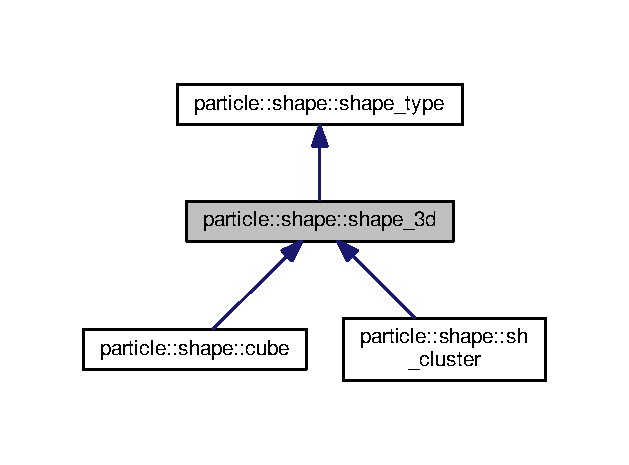
\includegraphics[width=302pt]{d4/dbf/classparticle_1_1shape_1_1shape__3d__inherit__graph}
\end{center}
\end{figure}


Collaboration diagram for particle\+:\+:shape\+:\+:shape\+\_\+3d\+:\nopagebreak
\begin{figure}[H]
\begin{center}
\leavevmode
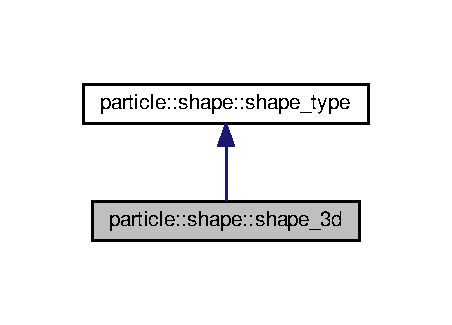
\includegraphics[width=217pt]{d1/d61/classparticle_1_1shape_1_1shape__3d__coll__graph}
\end{center}
\end{figure}
\subsection*{Public Member Functions}
\begin{DoxyCompactItemize}
\item 
\hyperlink{classparticle_1_1shape_1_1shape__3d_a5f7180f1f02937bf0b89e58229fb4848}{shape\+\_\+3d} ()
\begin{DoxyCompactList}\small\item\em Default constructor. \end{DoxyCompactList}\item 
\hyperlink{classparticle_1_1shape_1_1shape__3d_a9870c53de9607e6684f839f7b55058f9}{$\sim$shape\+\_\+3d} ()
\begin{DoxyCompactList}\small\item\em Default destructor. \end{DoxyCompactList}\item 
virtual bool \hyperlink{classparticle_1_1shape_1_1shape__3d_afa0d3025b8446a142b8979065eeb6379}{check} (std\+::vector$<$ int $>$ Is, int l\+\_\+size)
\begin{DoxyCompactList}\small\item\em Check whether a certain position falls within the particle. \end{DoxyCompactList}\end{DoxyCompactItemize}


\subsection{Detailed Description}
3D particle shapes. 

\subsection{Constructor \& Destructor Documentation}
\index{particle\+::shape\+::shape\+\_\+3d@{particle\+::shape\+::shape\+\_\+3d}!shape\+\_\+3d@{shape\+\_\+3d}}
\index{shape\+\_\+3d@{shape\+\_\+3d}!particle\+::shape\+::shape\+\_\+3d@{particle\+::shape\+::shape\+\_\+3d}}
\subsubsection[{\texorpdfstring{shape\+\_\+3d()}{shape_3d()}}]{\setlength{\rightskip}{0pt plus 5cm}particle\+::shape\+::shape\+\_\+3d\+::shape\+\_\+3d (
\begin{DoxyParamCaption}
{}
\end{DoxyParamCaption}
)\hspace{0.3cm}{\ttfamily [inline]}}\hypertarget{classparticle_1_1shape_1_1shape__3d_a5f7180f1f02937bf0b89e58229fb4848}{}\label{classparticle_1_1shape_1_1shape__3d_a5f7180f1f02937bf0b89e58229fb4848}


Default constructor. 

\index{particle\+::shape\+::shape\+\_\+3d@{particle\+::shape\+::shape\+\_\+3d}!````~shape\+\_\+3d@{$\sim$shape\+\_\+3d}}
\index{````~shape\+\_\+3d@{$\sim$shape\+\_\+3d}!particle\+::shape\+::shape\+\_\+3d@{particle\+::shape\+::shape\+\_\+3d}}
\subsubsection[{\texorpdfstring{$\sim$shape\+\_\+3d()}{~shape_3d()}}]{\setlength{\rightskip}{0pt plus 5cm}particle\+::shape\+::shape\+\_\+3d\+::$\sim$shape\+\_\+3d (
\begin{DoxyParamCaption}
{}
\end{DoxyParamCaption}
)\hspace{0.3cm}{\ttfamily [inline]}}\hypertarget{classparticle_1_1shape_1_1shape__3d_a9870c53de9607e6684f839f7b55058f9}{}\label{classparticle_1_1shape_1_1shape__3d_a9870c53de9607e6684f839f7b55058f9}


Default destructor. 



\subsection{Member Function Documentation}
\index{particle\+::shape\+::shape\+\_\+3d@{particle\+::shape\+::shape\+\_\+3d}!check@{check}}
\index{check@{check}!particle\+::shape\+::shape\+\_\+3d@{particle\+::shape\+::shape\+\_\+3d}}
\subsubsection[{\texorpdfstring{check(std\+::vector$<$ int $>$ Is, int l\+\_\+size)}{check(std::vector< int > Is, int l_size)}}]{\setlength{\rightskip}{0pt plus 5cm}virtual bool particle\+::shape\+::shape\+\_\+3d\+::check (
\begin{DoxyParamCaption}
\item[{std\+::vector$<$ int $>$}]{Is, }
\item[{int}]{l\+\_\+size}
\end{DoxyParamCaption}
)\hspace{0.3cm}{\ttfamily [inline]}, {\ttfamily [virtual]}}\hypertarget{classparticle_1_1shape_1_1shape__3d_afa0d3025b8446a142b8979065eeb6379}{}\label{classparticle_1_1shape_1_1shape__3d_afa0d3025b8446a142b8979065eeb6379}


Check whether a certain position falls within the particle. 


\begin{DoxyParams}{Parameters}
{\em Is} & The coordinates of the lattice site. \\
\hline
{\em l\+\_\+size} & The total lattice size. \\
\hline
\end{DoxyParams}


Reimplemented from \hyperlink{classparticle_1_1shape_1_1shape__type_a64d04f49c8da656d8b8899c431c346fc}{particle\+::shape\+::shape\+\_\+type}.



The documentation for this class was generated from the following file\+:\begin{DoxyCompactItemize}
\item 
includes/\hyperlink{shape_8hpp}{shape.\+hpp}\end{DoxyCompactItemize}

\hypertarget{classparticle_1_1shape_1_1shape__type}{}\section{particle\+:\+:shape\+:\+:shape\+\_\+type Class Reference}
\label{classparticle_1_1shape_1_1shape__type}\index{particle\+::shape\+::shape\+\_\+type@{particle\+::shape\+::shape\+\_\+type}}


Base class for particle shapes.  




{\ttfamily \#include $<$shape.\+hpp$>$}



Inheritance diagram for particle\+:\+:shape\+:\+:shape\+\_\+type\+:\nopagebreak
\begin{figure}[H]
\begin{center}
\leavevmode
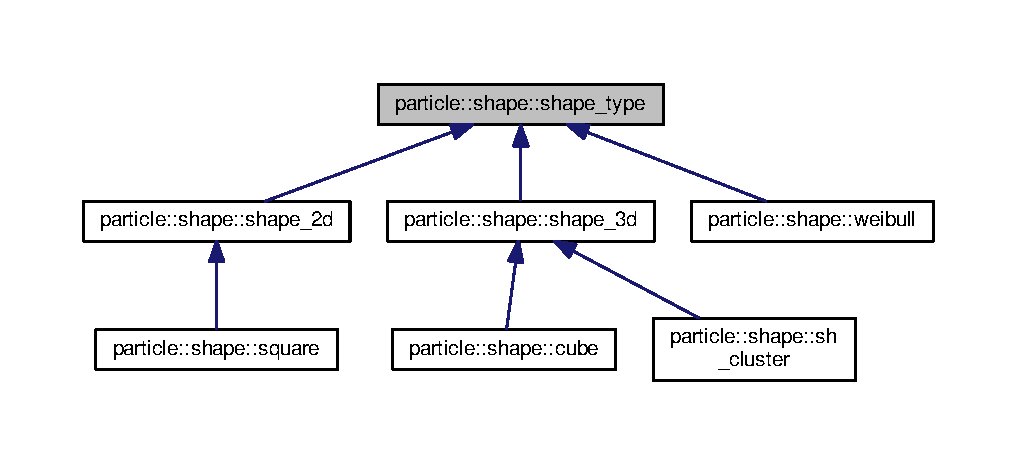
\includegraphics[width=350pt]{d6/d08/classparticle_1_1shape_1_1shape__type__inherit__graph}
\end{center}
\end{figure}
\subsection*{Public Member Functions}
\begin{DoxyCompactItemize}
\item 
\hyperlink{classparticle_1_1shape_1_1shape__type_ab187327a7f6a06f60f4714395f3eca88}{shape\+\_\+type} ()
\begin{DoxyCompactList}\small\item\em Default constructor. \end{DoxyCompactList}\item 
\hyperlink{classparticle_1_1shape_1_1shape__type_a86b549bc6531e04873ca057172ec3f0f}{$\sim$shape\+\_\+type} ()
\begin{DoxyCompactList}\small\item\em Default destructor. \end{DoxyCompactList}\item 
virtual bool \hyperlink{classparticle_1_1shape_1_1shape__type_a64d04f49c8da656d8b8899c431c346fc}{check} (std\+::vector$<$ int $>$ Is, int l\+\_\+size)
\begin{DoxyCompactList}\small\item\em Check whether a certain position falls within the particle. \end{DoxyCompactList}\item 
virtual double \hyperlink{classparticle_1_1shape_1_1shape__type_a062dfaf9cbfe98cdcdc55c34a0463313}{get\+\_\+r0} ()
\begin{DoxyCompactList}\small\item\em Returns the characteristic size of a weibull particle. \end{DoxyCompactList}\item 
virtual double \hyperlink{classparticle_1_1shape_1_1shape__type_a041dd08774f26ffeeb051e1442cb612c}{get\+\_\+beta} ()
\begin{DoxyCompactList}\small\item\em Returns the disorder parameter of a weibull particle. \end{DoxyCompactList}\item 
virtual double \hyperlink{classparticle_1_1shape_1_1shape__type_a7b938aa8c2dada71e8d0b11c6a676449}{get\+\_\+a} ()
\begin{DoxyCompactList}\small\item\em Returns the x-\/axis radius of a weibull particle. \end{DoxyCompactList}\item 
virtual double \hyperlink{classparticle_1_1shape_1_1shape__type_a0a9f0a397edbc66120114c89a185c127}{get\+\_\+b} ()
\begin{DoxyCompactList}\small\item\em Returns the y-\/axis radius of a weibull particle. \end{DoxyCompactList}\item 
virtual double \hyperlink{classparticle_1_1shape_1_1shape__type_a4f37d43b6e014a429e45480cea48f63d}{get\+\_\+c} ()
\begin{DoxyCompactList}\small\item\em Returns the z-\/axis radius of a weibull particle. \end{DoxyCompactList}\end{DoxyCompactItemize}


\subsection{Detailed Description}
Base class for particle shapes. 

\subsection{Constructor \& Destructor Documentation}
\index{particle\+::shape\+::shape\+\_\+type@{particle\+::shape\+::shape\+\_\+type}!shape\+\_\+type@{shape\+\_\+type}}
\index{shape\+\_\+type@{shape\+\_\+type}!particle\+::shape\+::shape\+\_\+type@{particle\+::shape\+::shape\+\_\+type}}
\subsubsection[{\texorpdfstring{shape\+\_\+type()}{shape_type()}}]{\setlength{\rightskip}{0pt plus 5cm}particle\+::shape\+::shape\+\_\+type\+::shape\+\_\+type (
\begin{DoxyParamCaption}
{}
\end{DoxyParamCaption}
)\hspace{0.3cm}{\ttfamily [inline]}}\hypertarget{classparticle_1_1shape_1_1shape__type_ab187327a7f6a06f60f4714395f3eca88}{}\label{classparticle_1_1shape_1_1shape__type_ab187327a7f6a06f60f4714395f3eca88}


Default constructor. 

\index{particle\+::shape\+::shape\+\_\+type@{particle\+::shape\+::shape\+\_\+type}!````~shape\+\_\+type@{$\sim$shape\+\_\+type}}
\index{````~shape\+\_\+type@{$\sim$shape\+\_\+type}!particle\+::shape\+::shape\+\_\+type@{particle\+::shape\+::shape\+\_\+type}}
\subsubsection[{\texorpdfstring{$\sim$shape\+\_\+type()}{~shape_type()}}]{\setlength{\rightskip}{0pt plus 5cm}particle\+::shape\+::shape\+\_\+type\+::$\sim$shape\+\_\+type (
\begin{DoxyParamCaption}
{}
\end{DoxyParamCaption}
)\hspace{0.3cm}{\ttfamily [inline]}}\hypertarget{classparticle_1_1shape_1_1shape__type_a86b549bc6531e04873ca057172ec3f0f}{}\label{classparticle_1_1shape_1_1shape__type_a86b549bc6531e04873ca057172ec3f0f}


Default destructor. 



\subsection{Member Function Documentation}
\index{particle\+::shape\+::shape\+\_\+type@{particle\+::shape\+::shape\+\_\+type}!check@{check}}
\index{check@{check}!particle\+::shape\+::shape\+\_\+type@{particle\+::shape\+::shape\+\_\+type}}
\subsubsection[{\texorpdfstring{check(std\+::vector$<$ int $>$ Is, int l\+\_\+size)}{check(std::vector< int > Is, int l_size)}}]{\setlength{\rightskip}{0pt plus 5cm}virtual bool particle\+::shape\+::shape\+\_\+type\+::check (
\begin{DoxyParamCaption}
\item[{std\+::vector$<$ int $>$}]{Is, }
\item[{int}]{l\+\_\+size}
\end{DoxyParamCaption}
)\hspace{0.3cm}{\ttfamily [inline]}, {\ttfamily [virtual]}}\hypertarget{classparticle_1_1shape_1_1shape__type_a64d04f49c8da656d8b8899c431c346fc}{}\label{classparticle_1_1shape_1_1shape__type_a64d04f49c8da656d8b8899c431c346fc}


Check whether a certain position falls within the particle. 


\begin{DoxyParams}{Parameters}
{\em Is} & The coordinates of the lattice site. \\
\hline
{\em l\+\_\+size} & The total lattice size. \\
\hline
\end{DoxyParams}


Reimplemented in \hyperlink{classparticle_1_1shape_1_1weibull_a22612311ce2f3ca4317f8263e52de425}{particle\+::shape\+::weibull}, \hyperlink{classparticle_1_1shape_1_1shape__3d_afa0d3025b8446a142b8979065eeb6379}{particle\+::shape\+::shape\+\_\+3d}, and \hyperlink{classparticle_1_1shape_1_1shape__2d_a756e06b46afd0e18d6a37a0a8f28551c}{particle\+::shape\+::shape\+\_\+2d}.

\index{particle\+::shape\+::shape\+\_\+type@{particle\+::shape\+::shape\+\_\+type}!get\+\_\+a@{get\+\_\+a}}
\index{get\+\_\+a@{get\+\_\+a}!particle\+::shape\+::shape\+\_\+type@{particle\+::shape\+::shape\+\_\+type}}
\subsubsection[{\texorpdfstring{get\+\_\+a()}{get_a()}}]{\setlength{\rightskip}{0pt plus 5cm}virtual double particle\+::shape\+::shape\+\_\+type\+::get\+\_\+a (
\begin{DoxyParamCaption}
{}
\end{DoxyParamCaption}
)\hspace{0.3cm}{\ttfamily [inline]}, {\ttfamily [virtual]}}\hypertarget{classparticle_1_1shape_1_1shape__type_a7b938aa8c2dada71e8d0b11c6a676449}{}\label{classparticle_1_1shape_1_1shape__type_a7b938aa8c2dada71e8d0b11c6a676449}


Returns the x-\/axis radius of a weibull particle. 



Reimplemented in \hyperlink{classparticle_1_1shape_1_1weibull_a0234fa42b67465c7191248f524f27a0e}{particle\+::shape\+::weibull}.

\index{particle\+::shape\+::shape\+\_\+type@{particle\+::shape\+::shape\+\_\+type}!get\+\_\+b@{get\+\_\+b}}
\index{get\+\_\+b@{get\+\_\+b}!particle\+::shape\+::shape\+\_\+type@{particle\+::shape\+::shape\+\_\+type}}
\subsubsection[{\texorpdfstring{get\+\_\+b()}{get_b()}}]{\setlength{\rightskip}{0pt plus 5cm}virtual double particle\+::shape\+::shape\+\_\+type\+::get\+\_\+b (
\begin{DoxyParamCaption}
{}
\end{DoxyParamCaption}
)\hspace{0.3cm}{\ttfamily [inline]}, {\ttfamily [virtual]}}\hypertarget{classparticle_1_1shape_1_1shape__type_a0a9f0a397edbc66120114c89a185c127}{}\label{classparticle_1_1shape_1_1shape__type_a0a9f0a397edbc66120114c89a185c127}


Returns the y-\/axis radius of a weibull particle. 



Reimplemented in \hyperlink{classparticle_1_1shape_1_1weibull_a1066adcab828f8636475128ff51c56f0}{particle\+::shape\+::weibull}.

\index{particle\+::shape\+::shape\+\_\+type@{particle\+::shape\+::shape\+\_\+type}!get\+\_\+beta@{get\+\_\+beta}}
\index{get\+\_\+beta@{get\+\_\+beta}!particle\+::shape\+::shape\+\_\+type@{particle\+::shape\+::shape\+\_\+type}}
\subsubsection[{\texorpdfstring{get\+\_\+beta()}{get_beta()}}]{\setlength{\rightskip}{0pt plus 5cm}virtual double particle\+::shape\+::shape\+\_\+type\+::get\+\_\+beta (
\begin{DoxyParamCaption}
{}
\end{DoxyParamCaption}
)\hspace{0.3cm}{\ttfamily [inline]}, {\ttfamily [virtual]}}\hypertarget{classparticle_1_1shape_1_1shape__type_a041dd08774f26ffeeb051e1442cb612c}{}\label{classparticle_1_1shape_1_1shape__type_a041dd08774f26ffeeb051e1442cb612c}


Returns the disorder parameter of a weibull particle. 



Reimplemented in \hyperlink{classparticle_1_1shape_1_1weibull_a640180ce2bd6ce7f68c10d4791bce49c}{particle\+::shape\+::weibull}.

\index{particle\+::shape\+::shape\+\_\+type@{particle\+::shape\+::shape\+\_\+type}!get\+\_\+c@{get\+\_\+c}}
\index{get\+\_\+c@{get\+\_\+c}!particle\+::shape\+::shape\+\_\+type@{particle\+::shape\+::shape\+\_\+type}}
\subsubsection[{\texorpdfstring{get\+\_\+c()}{get_c()}}]{\setlength{\rightskip}{0pt plus 5cm}virtual double particle\+::shape\+::shape\+\_\+type\+::get\+\_\+c (
\begin{DoxyParamCaption}
{}
\end{DoxyParamCaption}
)\hspace{0.3cm}{\ttfamily [inline]}, {\ttfamily [virtual]}}\hypertarget{classparticle_1_1shape_1_1shape__type_a4f37d43b6e014a429e45480cea48f63d}{}\label{classparticle_1_1shape_1_1shape__type_a4f37d43b6e014a429e45480cea48f63d}


Returns the z-\/axis radius of a weibull particle. 



Reimplemented in \hyperlink{classparticle_1_1shape_1_1weibull_a0b8c38944e502df7bce4e8f99d149237}{particle\+::shape\+::weibull}.

\index{particle\+::shape\+::shape\+\_\+type@{particle\+::shape\+::shape\+\_\+type}!get\+\_\+r0@{get\+\_\+r0}}
\index{get\+\_\+r0@{get\+\_\+r0}!particle\+::shape\+::shape\+\_\+type@{particle\+::shape\+::shape\+\_\+type}}
\subsubsection[{\texorpdfstring{get\+\_\+r0()}{get_r0()}}]{\setlength{\rightskip}{0pt plus 5cm}virtual double particle\+::shape\+::shape\+\_\+type\+::get\+\_\+r0 (
\begin{DoxyParamCaption}
{}
\end{DoxyParamCaption}
)\hspace{0.3cm}{\ttfamily [inline]}, {\ttfamily [virtual]}}\hypertarget{classparticle_1_1shape_1_1shape__type_a062dfaf9cbfe98cdcdc55c34a0463313}{}\label{classparticle_1_1shape_1_1shape__type_a062dfaf9cbfe98cdcdc55c34a0463313}


Returns the characteristic size of a weibull particle. 



Reimplemented in \hyperlink{classparticle_1_1shape_1_1weibull_a85ab45f804ae9aa3fb712c435125ff70}{particle\+::shape\+::weibull}.



The documentation for this class was generated from the following file\+:\begin{DoxyCompactItemize}
\item 
includes/\hyperlink{shape_8hpp}{shape.\+hpp}\end{DoxyCompactItemize}

\hypertarget{classparticle_1_1shape_1_1square}{}\section{particle\+:\+:shape\+:\+:square Class Reference}
\label{classparticle_1_1shape_1_1square}\index{particle\+::shape\+::square@{particle\+::shape\+::square}}


Square particle.  




{\ttfamily \#include $<$shape.\+hpp$>$}



Inheritance diagram for particle\+:\+:shape\+:\+:square\+:\nopagebreak
\begin{figure}[H]
\begin{center}
\leavevmode
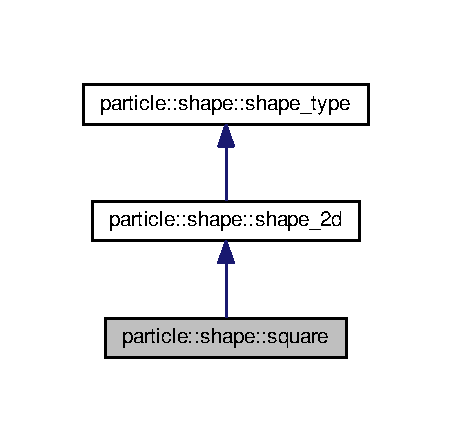
\includegraphics[width=217pt]{dd/d48/classparticle_1_1shape_1_1square__inherit__graph}
\end{center}
\end{figure}


Collaboration diagram for particle\+:\+:shape\+:\+:square\+:\nopagebreak
\begin{figure}[H]
\begin{center}
\leavevmode
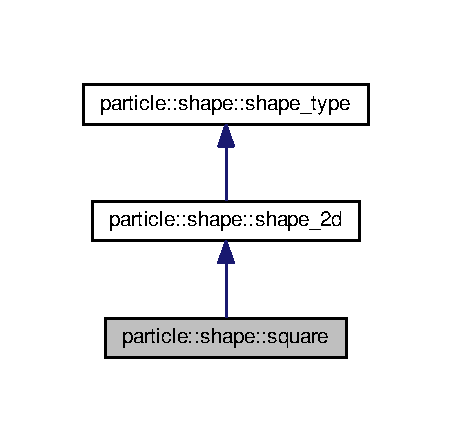
\includegraphics[width=217pt]{dd/d79/classparticle_1_1shape_1_1square__coll__graph}
\end{center}
\end{figure}
\subsection*{Public Member Functions}
\begin{DoxyCompactItemize}
\item 
\hyperlink{classparticle_1_1shape_1_1square_ad20d36cae1a25b17f151e194cca2933a}{square} ()
\begin{DoxyCompactList}\small\item\em Default constructor. \end{DoxyCompactList}\item 
\hyperlink{classparticle_1_1shape_1_1square_a2c16c3c04400bc8db355ea4d0ed2d2ec}{$\sim$square} ()
\begin{DoxyCompactList}\small\item\em Default destructor. \end{DoxyCompactList}\end{DoxyCompactItemize}


\subsection{Detailed Description}
Square particle. 

\subsection{Constructor \& Destructor Documentation}
\index{particle\+::shape\+::square@{particle\+::shape\+::square}!square@{square}}
\index{square@{square}!particle\+::shape\+::square@{particle\+::shape\+::square}}
\subsubsection[{\texorpdfstring{square()}{square()}}]{\setlength{\rightskip}{0pt plus 5cm}particle\+::shape\+::square\+::square (
\begin{DoxyParamCaption}
{}
\end{DoxyParamCaption}
)\hspace{0.3cm}{\ttfamily [inline]}}\hypertarget{classparticle_1_1shape_1_1square_ad20d36cae1a25b17f151e194cca2933a}{}\label{classparticle_1_1shape_1_1square_ad20d36cae1a25b17f151e194cca2933a}


Default constructor. 

\index{particle\+::shape\+::square@{particle\+::shape\+::square}!````~square@{$\sim$square}}
\index{````~square@{$\sim$square}!particle\+::shape\+::square@{particle\+::shape\+::square}}
\subsubsection[{\texorpdfstring{$\sim$square()}{~square()}}]{\setlength{\rightskip}{0pt plus 5cm}particle\+::shape\+::square\+::$\sim$square (
\begin{DoxyParamCaption}
{}
\end{DoxyParamCaption}
)\hspace{0.3cm}{\ttfamily [inline]}}\hypertarget{classparticle_1_1shape_1_1square_a2c16c3c04400bc8db355ea4d0ed2d2ec}{}\label{classparticle_1_1shape_1_1square_a2c16c3c04400bc8db355ea4d0ed2d2ec}


Default destructor. 



The documentation for this class was generated from the following file\+:\begin{DoxyCompactItemize}
\item 
includes/\hyperlink{shape_8hpp}{shape.\+hpp}\end{DoxyCompactItemize}

\hypertarget{classstate}{}\section{state Class Reference}
\label{classstate}\index{state@{state}}


{\ttfamily \#include $<$state.\+hpp$>$}

\subsection*{Public Member Functions}
\begin{DoxyCompactItemize}
\item 
\hyperlink{classstate_aee920d9f534640451f22b3525f9cb9de}{state} ()
\item 
\hyperlink{classstate_aa3dee783102d59b3c07617558c25afaf}{state} (\hyperlink{structstateOptions}{state\+Options} opt)
\item 
\hyperlink{classstate_a285d976cdbd4a9de9ec8d1d887991ecc}{state} (const \hyperlink{classstate}{state} \&other)
\item 
\hyperlink{classstate_a60216b51b01ca0ebe9786ec2da66568f}{$\sim$state} ()
\item 
\hyperlink{classparticle_1_1field_1_1field__type}{particle\+::field\+::field\+\_\+type} \hyperlink{classstate_a0a6f3f9510acca9b766cc4b4f17671c0}{get\+\_\+field} ()
\item 
void \hyperlink{classstate_a0d0ea6448509ececead44d83b4decd1c}{copy\+\_\+points} (const \hyperlink{classstate}{state} \&other)
\item 
void \hyperlink{classstate_aac3b2330539154d3784730e4c8a61123}{init\+\_\+points} (\hyperlink{structstateOptions}{state\+Options} opt)
\item 
void \hyperlink{classstate_af70b6f999313cc427a526388058cb45c}{equil} (int iter)
\item 
std\+::vector$<$ double $>$ \hyperlink{classstate_a5d5980e59b16063808f09eac46d14292}{magnetisation} ()
\item 
std\+::vector$<$ double $>$ \hyperlink{classstate_aff62d62706dc27dde2c3638769c0a00a}{submag} (int subnumber)
\item 
double \hyperlink{classstate_a6209503f752e5089e0301f103fdf1d1e}{energy} ()
\item 
std\+::vector$<$ double $>$ \hyperlink{classstate_aba4b4f47fc3b9cba97b5f63518214f30}{tcharge} ()
\item 
int \hyperlink{classstate_ad9182b875a7a3fb5981c811f7f062040}{num\+\_\+spins} ()
\item 
int \hyperlink{classstate_acf2ec1dfdb1068a279de590375cbcb96}{get\+\_\+size} ()
\item 
int \hyperlink{classstate_a8351befda232e04536d6a3e738754282}{sub\+\_\+num} (int subnumber)
\item 
void \hyperlink{classstate_acfeea4e197f5ce0160c6c664740ba6ff}{init\+\_\+lattice} ()
\item 
void \hyperlink{classstate_aca18a3757a2e6bd79cda366e4e31bb99}{change\+\_\+temp} (double T)
\item 
void \hyperlink{classstate_a3f54c8647fddb251db2ba11420f4e75f}{change\+\_\+field} (double Hin)
\item 
\hyperlink{classstate}{state} \& \hyperlink{classstate_a8f382a578a92617e7294cbbd80fba3c6}{operator=} (const \hyperlink{classstate}{state} \&other)
\item 
void \hyperlink{classstate_afa18f63b166492174bf88cd52c1cb748}{print\+\_\+latt} ()
\item 
void \hyperlink{classstate_af478dc8ce44c65cc535530738693eff5}{ptf} (std\+::string fname, std\+::string arrname)
\item 
void \hyperlink{classstate_a2d9073df186ccbf4159022d1c8c3b061}{add\+\_\+to\+\_\+av} (\hyperlink{classparticle_1_1field_1_1field__type}{particle\+::field\+::field\+\_\+type} \&other\+\_\+field)
\item 
void \hyperlink{classstate_a74588f49ec2b0868442d78ed9dcf1224}{change\+\_\+v1} (int protocol, double v1)
\item 
void \hyperlink{classstate_a9ffa7fbd21b542e66a9275f63b80ed0a}{change\+\_\+v2} (int protocol, double v2)
\item 
void \hyperlink{classstate_a6e35e024e6139032a54099bfe84a6fa4}{send\+\_\+latt\+\_\+data} (int dest\+\_\+rank)
\item 
void \hyperlink{classstate_a5ce0ea314795d1cc37849604f202fb98}{recv\+\_\+latt\+\_\+data} (int src\+\_\+rank)
\end{DoxyCompactItemize}


\subsection{Constructor \& Destructor Documentation}
\index{state@{state}!state@{state}}
\index{state@{state}!state@{state}}
\subsubsection[{\texorpdfstring{state()}{state()}}]{\setlength{\rightskip}{0pt plus 5cm}state\+::state (
\begin{DoxyParamCaption}
{}
\end{DoxyParamCaption}
)\hspace{0.3cm}{\ttfamily [inline]}}\hypertarget{classstate_aee920d9f534640451f22b3525f9cb9de}{}\label{classstate_aee920d9f534640451f22b3525f9cb9de}
\index{state@{state}!state@{state}}
\index{state@{state}!state@{state}}
\subsubsection[{\texorpdfstring{state(state\+Options opt)}{state(stateOptions opt)}}]{\setlength{\rightskip}{0pt plus 5cm}state\+::state (
\begin{DoxyParamCaption}
\item[{{\bf state\+Options}}]{opt}
\end{DoxyParamCaption}
)}\hypertarget{classstate_aa3dee783102d59b3c07617558c25afaf}{}\label{classstate_aa3dee783102d59b3c07617558c25afaf}
\index{state@{state}!state@{state}}
\index{state@{state}!state@{state}}
\subsubsection[{\texorpdfstring{state(const state \&other)}{state(const state &other)}}]{\setlength{\rightskip}{0pt plus 5cm}state\+::state (
\begin{DoxyParamCaption}
\item[{const {\bf state} \&}]{other}
\end{DoxyParamCaption}
)}\hypertarget{classstate_a285d976cdbd4a9de9ec8d1d887991ecc}{}\label{classstate_a285d976cdbd4a9de9ec8d1d887991ecc}
\index{state@{state}!````~state@{$\sim$state}}
\index{````~state@{$\sim$state}!state@{state}}
\subsubsection[{\texorpdfstring{$\sim$state()}{~state()}}]{\setlength{\rightskip}{0pt plus 5cm}state\+::$\sim$state (
\begin{DoxyParamCaption}
{}
\end{DoxyParamCaption}
)}\hypertarget{classstate_a60216b51b01ca0ebe9786ec2da66568f}{}\label{classstate_a60216b51b01ca0ebe9786ec2da66568f}


\subsection{Member Function Documentation}
\index{state@{state}!add\+\_\+to\+\_\+av@{add\+\_\+to\+\_\+av}}
\index{add\+\_\+to\+\_\+av@{add\+\_\+to\+\_\+av}!state@{state}}
\subsubsection[{\texorpdfstring{add\+\_\+to\+\_\+av(particle\+::field\+::field\+\_\+type \&other\+\_\+field)}{add_to_av(particle::field::field_type &other_field)}}]{\setlength{\rightskip}{0pt plus 5cm}void state\+::add\+\_\+to\+\_\+av (
\begin{DoxyParamCaption}
\item[{{\bf particle\+::field\+::field\+\_\+type} \&}]{other\+\_\+field}
\end{DoxyParamCaption}
)}\hypertarget{classstate_a2d9073df186ccbf4159022d1c8c3b061}{}\label{classstate_a2d9073df186ccbf4159022d1c8c3b061}
\index{state@{state}!change\+\_\+field@{change\+\_\+field}}
\index{change\+\_\+field@{change\+\_\+field}!state@{state}}
\subsubsection[{\texorpdfstring{change\+\_\+field(double Hin)}{change_field(double Hin)}}]{\setlength{\rightskip}{0pt plus 5cm}void state\+::change\+\_\+field (
\begin{DoxyParamCaption}
\item[{double}]{Hin}
\end{DoxyParamCaption}
)}\hypertarget{classstate_a3f54c8647fddb251db2ba11420f4e75f}{}\label{classstate_a3f54c8647fddb251db2ba11420f4e75f}
\index{state@{state}!change\+\_\+temp@{change\+\_\+temp}}
\index{change\+\_\+temp@{change\+\_\+temp}!state@{state}}
\subsubsection[{\texorpdfstring{change\+\_\+temp(double T)}{change_temp(double T)}}]{\setlength{\rightskip}{0pt plus 5cm}void state\+::change\+\_\+temp (
\begin{DoxyParamCaption}
\item[{double}]{T}
\end{DoxyParamCaption}
)}\hypertarget{classstate_aca18a3757a2e6bd79cda366e4e31bb99}{}\label{classstate_aca18a3757a2e6bd79cda366e4e31bb99}
\index{state@{state}!change\+\_\+v1@{change\+\_\+v1}}
\index{change\+\_\+v1@{change\+\_\+v1}!state@{state}}
\subsubsection[{\texorpdfstring{change\+\_\+v1(int protocol, double v1)}{change_v1(int protocol, double v1)}}]{\setlength{\rightskip}{0pt plus 5cm}void state\+::change\+\_\+v1 (
\begin{DoxyParamCaption}
\item[{int}]{protocol, }
\item[{double}]{v1}
\end{DoxyParamCaption}
)}\hypertarget{classstate_a74588f49ec2b0868442d78ed9dcf1224}{}\label{classstate_a74588f49ec2b0868442d78ed9dcf1224}
\index{state@{state}!change\+\_\+v2@{change\+\_\+v2}}
\index{change\+\_\+v2@{change\+\_\+v2}!state@{state}}
\subsubsection[{\texorpdfstring{change\+\_\+v2(int protocol, double v2)}{change_v2(int protocol, double v2)}}]{\setlength{\rightskip}{0pt plus 5cm}void state\+::change\+\_\+v2 (
\begin{DoxyParamCaption}
\item[{int}]{protocol, }
\item[{double}]{v2}
\end{DoxyParamCaption}
)}\hypertarget{classstate_a9ffa7fbd21b542e66a9275f63b80ed0a}{}\label{classstate_a9ffa7fbd21b542e66a9275f63b80ed0a}
\index{state@{state}!copy\+\_\+points@{copy\+\_\+points}}
\index{copy\+\_\+points@{copy\+\_\+points}!state@{state}}
\subsubsection[{\texorpdfstring{copy\+\_\+points(const state \&other)}{copy_points(const state &other)}}]{\setlength{\rightskip}{0pt plus 5cm}void state\+::copy\+\_\+points (
\begin{DoxyParamCaption}
\item[{const {\bf state} \&}]{other}
\end{DoxyParamCaption}
)}\hypertarget{classstate_a0d0ea6448509ececead44d83b4decd1c}{}\label{classstate_a0d0ea6448509ececead44d83b4decd1c}
\index{state@{state}!energy@{energy}}
\index{energy@{energy}!state@{state}}
\subsubsection[{\texorpdfstring{energy()}{energy()}}]{\setlength{\rightskip}{0pt plus 5cm}double state\+::energy (
\begin{DoxyParamCaption}
{}
\end{DoxyParamCaption}
)}\hypertarget{classstate_a6209503f752e5089e0301f103fdf1d1e}{}\label{classstate_a6209503f752e5089e0301f103fdf1d1e}
\index{state@{state}!equil@{equil}}
\index{equil@{equil}!state@{state}}
\subsubsection[{\texorpdfstring{equil(int iter)}{equil(int iter)}}]{\setlength{\rightskip}{0pt plus 5cm}void state\+::equil (
\begin{DoxyParamCaption}
\item[{int}]{iter}
\end{DoxyParamCaption}
)}\hypertarget{classstate_af70b6f999313cc427a526388058cb45c}{}\label{classstate_af70b6f999313cc427a526388058cb45c}
\index{state@{state}!get\+\_\+field@{get\+\_\+field}}
\index{get\+\_\+field@{get\+\_\+field}!state@{state}}
\subsubsection[{\texorpdfstring{get\+\_\+field()}{get_field()}}]{\setlength{\rightskip}{0pt plus 5cm}{\bf particle\+::field\+::field\+\_\+type} state\+::get\+\_\+field (
\begin{DoxyParamCaption}
{}
\end{DoxyParamCaption}
)\hspace{0.3cm}{\ttfamily [inline]}}\hypertarget{classstate_a0a6f3f9510acca9b766cc4b4f17671c0}{}\label{classstate_a0a6f3f9510acca9b766cc4b4f17671c0}
\index{state@{state}!get\+\_\+size@{get\+\_\+size}}
\index{get\+\_\+size@{get\+\_\+size}!state@{state}}
\subsubsection[{\texorpdfstring{get\+\_\+size()}{get_size()}}]{\setlength{\rightskip}{0pt plus 5cm}int state\+::get\+\_\+size (
\begin{DoxyParamCaption}
{}
\end{DoxyParamCaption}
)\hspace{0.3cm}{\ttfamily [inline]}}\hypertarget{classstate_acf2ec1dfdb1068a279de590375cbcb96}{}\label{classstate_acf2ec1dfdb1068a279de590375cbcb96}
\index{state@{state}!init\+\_\+lattice@{init\+\_\+lattice}}
\index{init\+\_\+lattice@{init\+\_\+lattice}!state@{state}}
\subsubsection[{\texorpdfstring{init\+\_\+lattice()}{init_lattice()}}]{\setlength{\rightskip}{0pt plus 5cm}void state\+::init\+\_\+lattice (
\begin{DoxyParamCaption}
{}
\end{DoxyParamCaption}
)}\hypertarget{classstate_acfeea4e197f5ce0160c6c664740ba6ff}{}\label{classstate_acfeea4e197f5ce0160c6c664740ba6ff}
\index{state@{state}!init\+\_\+points@{init\+\_\+points}}
\index{init\+\_\+points@{init\+\_\+points}!state@{state}}
\subsubsection[{\texorpdfstring{init\+\_\+points(state\+Options opt)}{init_points(stateOptions opt)}}]{\setlength{\rightskip}{0pt plus 5cm}void state\+::init\+\_\+points (
\begin{DoxyParamCaption}
\item[{{\bf state\+Options}}]{opt}
\end{DoxyParamCaption}
)}\hypertarget{classstate_aac3b2330539154d3784730e4c8a61123}{}\label{classstate_aac3b2330539154d3784730e4c8a61123}
\index{state@{state}!magnetisation@{magnetisation}}
\index{magnetisation@{magnetisation}!state@{state}}
\subsubsection[{\texorpdfstring{magnetisation()}{magnetisation()}}]{\setlength{\rightskip}{0pt plus 5cm}std\+::vector$<$double$>$ state\+::magnetisation (
\begin{DoxyParamCaption}
{}
\end{DoxyParamCaption}
)}\hypertarget{classstate_a5d5980e59b16063808f09eac46d14292}{}\label{classstate_a5d5980e59b16063808f09eac46d14292}
\index{state@{state}!num\+\_\+spins@{num\+\_\+spins}}
\index{num\+\_\+spins@{num\+\_\+spins}!state@{state}}
\subsubsection[{\texorpdfstring{num\+\_\+spins()}{num_spins()}}]{\setlength{\rightskip}{0pt plus 5cm}int state\+::num\+\_\+spins (
\begin{DoxyParamCaption}
{}
\end{DoxyParamCaption}
)}\hypertarget{classstate_ad9182b875a7a3fb5981c811f7f062040}{}\label{classstate_ad9182b875a7a3fb5981c811f7f062040}
\index{state@{state}!operator=@{operator=}}
\index{operator=@{operator=}!state@{state}}
\subsubsection[{\texorpdfstring{operator=(const state \&other)}{operator=(const state &other)}}]{\setlength{\rightskip}{0pt plus 5cm}{\bf state}\& state\+::operator= (
\begin{DoxyParamCaption}
\item[{const {\bf state} \&}]{other}
\end{DoxyParamCaption}
)}\hypertarget{classstate_a8f382a578a92617e7294cbbd80fba3c6}{}\label{classstate_a8f382a578a92617e7294cbbd80fba3c6}
\index{state@{state}!print\+\_\+latt@{print\+\_\+latt}}
\index{print\+\_\+latt@{print\+\_\+latt}!state@{state}}
\subsubsection[{\texorpdfstring{print\+\_\+latt()}{print_latt()}}]{\setlength{\rightskip}{0pt plus 5cm}void state\+::print\+\_\+latt (
\begin{DoxyParamCaption}
{}
\end{DoxyParamCaption}
)}\hypertarget{classstate_afa18f63b166492174bf88cd52c1cb748}{}\label{classstate_afa18f63b166492174bf88cd52c1cb748}
\index{state@{state}!ptf@{ptf}}
\index{ptf@{ptf}!state@{state}}
\subsubsection[{\texorpdfstring{ptf(std\+::string fname, std\+::string arrname)}{ptf(std::string fname, std::string arrname)}}]{\setlength{\rightskip}{0pt plus 5cm}void state\+::ptf (
\begin{DoxyParamCaption}
\item[{std\+::string}]{fname, }
\item[{std\+::string}]{arrname}
\end{DoxyParamCaption}
)}\hypertarget{classstate_af478dc8ce44c65cc535530738693eff5}{}\label{classstate_af478dc8ce44c65cc535530738693eff5}
\index{state@{state}!recv\+\_\+latt\+\_\+data@{recv\+\_\+latt\+\_\+data}}
\index{recv\+\_\+latt\+\_\+data@{recv\+\_\+latt\+\_\+data}!state@{state}}
\subsubsection[{\texorpdfstring{recv\+\_\+latt\+\_\+data(int src\+\_\+rank)}{recv_latt_data(int src_rank)}}]{\setlength{\rightskip}{0pt plus 5cm}void state\+::recv\+\_\+latt\+\_\+data (
\begin{DoxyParamCaption}
\item[{int}]{src\+\_\+rank}
\end{DoxyParamCaption}
)}\hypertarget{classstate_a5ce0ea314795d1cc37849604f202fb98}{}\label{classstate_a5ce0ea314795d1cc37849604f202fb98}
\index{state@{state}!send\+\_\+latt\+\_\+data@{send\+\_\+latt\+\_\+data}}
\index{send\+\_\+latt\+\_\+data@{send\+\_\+latt\+\_\+data}!state@{state}}
\subsubsection[{\texorpdfstring{send\+\_\+latt\+\_\+data(int dest\+\_\+rank)}{send_latt_data(int dest_rank)}}]{\setlength{\rightskip}{0pt plus 5cm}void state\+::send\+\_\+latt\+\_\+data (
\begin{DoxyParamCaption}
\item[{int}]{dest\+\_\+rank}
\end{DoxyParamCaption}
)}\hypertarget{classstate_a6e35e024e6139032a54099bfe84a6fa4}{}\label{classstate_a6e35e024e6139032a54099bfe84a6fa4}
\index{state@{state}!sub\+\_\+num@{sub\+\_\+num}}
\index{sub\+\_\+num@{sub\+\_\+num}!state@{state}}
\subsubsection[{\texorpdfstring{sub\+\_\+num(int subnumber)}{sub_num(int subnumber)}}]{\setlength{\rightskip}{0pt plus 5cm}int state\+::sub\+\_\+num (
\begin{DoxyParamCaption}
\item[{int}]{subnumber}
\end{DoxyParamCaption}
)}\hypertarget{classstate_a8351befda232e04536d6a3e738754282}{}\label{classstate_a8351befda232e04536d6a3e738754282}
\index{state@{state}!submag@{submag}}
\index{submag@{submag}!state@{state}}
\subsubsection[{\texorpdfstring{submag(int subnumber)}{submag(int subnumber)}}]{\setlength{\rightskip}{0pt plus 5cm}std\+::vector$<$double$>$ state\+::submag (
\begin{DoxyParamCaption}
\item[{int}]{subnumber}
\end{DoxyParamCaption}
)}\hypertarget{classstate_aff62d62706dc27dde2c3638769c0a00a}{}\label{classstate_aff62d62706dc27dde2c3638769c0a00a}
\index{state@{state}!tcharge@{tcharge}}
\index{tcharge@{tcharge}!state@{state}}
\subsubsection[{\texorpdfstring{tcharge()}{tcharge()}}]{\setlength{\rightskip}{0pt plus 5cm}std\+::vector$<$double$>$ state\+::tcharge (
\begin{DoxyParamCaption}
{}
\end{DoxyParamCaption}
)}\hypertarget{classstate_aba4b4f47fc3b9cba97b5f63518214f30}{}\label{classstate_aba4b4f47fc3b9cba97b5f63518214f30}


The documentation for this class was generated from the following file\+:\begin{DoxyCompactItemize}
\item 
includes/\hyperlink{state_8hpp}{state.\+hpp}\end{DoxyCompactItemize}

\hypertarget{classstdrand_1_1std__d__unirand}{}\section{stdrand\+:\+:std\+\_\+d\+\_\+unirand Class Reference}
\label{classstdrand_1_1std__d__unirand}\index{stdrand\+::std\+\_\+d\+\_\+unirand@{stdrand\+::std\+\_\+d\+\_\+unirand}}


Generator for uniform numbers between 0 and 1.  




{\ttfamily \#include $<$stdrand.\+hpp$>$}



Inheritance diagram for stdrand\+:\+:std\+\_\+d\+\_\+unirand\+:
\nopagebreak
\begin{figure}[H]
\begin{center}
\leavevmode
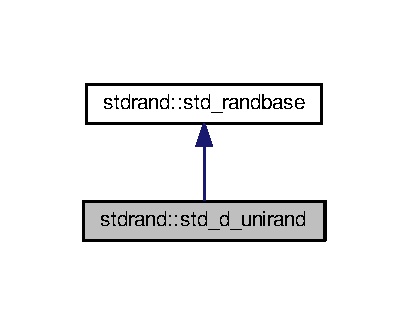
\includegraphics[width=196pt]{de/d88/classstdrand_1_1std__d__unirand__inherit__graph}
\end{center}
\end{figure}


Collaboration diagram for stdrand\+:\+:std\+\_\+d\+\_\+unirand\+:
\nopagebreak
\begin{figure}[H]
\begin{center}
\leavevmode
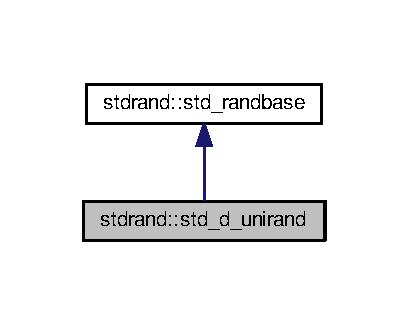
\includegraphics[width=196pt]{d2/dad/classstdrand_1_1std__d__unirand__coll__graph}
\end{center}
\end{figure}
\subsection*{Public Member Functions}
\begin{DoxyCompactItemize}
\item 
\hyperlink{classstdrand_1_1std__d__unirand_aae3235e8e1f6a1d28076899221687273}{std\+\_\+d\+\_\+unirand} (int seed)
\begin{DoxyCompactList}\small\item\em Constructor. \end{DoxyCompactList}\item 
\hyperlink{classstdrand_1_1std__d__unirand_add94ad2a131354549fe22f6f210d8278}{std\+\_\+d\+\_\+unirand} (int size, int seed)
\begin{DoxyCompactList}\small\item\em Constructor with dummy size input. \end{DoxyCompactList}\item 
\hyperlink{classstdrand_1_1std__d__unirand_a37784d8dca5fff875a77224b68cc931b}{$\sim$std\+\_\+d\+\_\+unirand} ()
\begin{DoxyCompactList}\small\item\em Default destructor. \end{DoxyCompactList}\item 
double \hyperlink{classstdrand_1_1std__d__unirand_a3dde71452da1a44bd6be86877e74be74}{gen} ()
\begin{DoxyCompactList}\small\item\em Return a single random number. \end{DoxyCompactList}\end{DoxyCompactItemize}
\subsection*{Additional Inherited Members}


\subsection{Detailed Description}
Generator for uniform numbers between 0 and 1. 

\subsection{Constructor \& Destructor Documentation}
\index{stdrand\+::std\+\_\+d\+\_\+unirand@{stdrand\+::std\+\_\+d\+\_\+unirand}!std\+\_\+d\+\_\+unirand@{std\+\_\+d\+\_\+unirand}}
\index{std\+\_\+d\+\_\+unirand@{std\+\_\+d\+\_\+unirand}!stdrand\+::std\+\_\+d\+\_\+unirand@{stdrand\+::std\+\_\+d\+\_\+unirand}}
\subsubsection[{\texorpdfstring{std\+\_\+d\+\_\+unirand(int seed)}{std_d_unirand(int seed)}}]{\setlength{\rightskip}{0pt plus 5cm}stdrand\+::std\+\_\+d\+\_\+unirand\+::std\+\_\+d\+\_\+unirand (
\begin{DoxyParamCaption}
\item[{int}]{seed}
\end{DoxyParamCaption}
)}\hypertarget{classstdrand_1_1std__d__unirand_aae3235e8e1f6a1d28076899221687273}{}\label{classstdrand_1_1std__d__unirand_aae3235e8e1f6a1d28076899221687273}


Constructor. 


\begin{DoxyParams}{Parameters}
{\em seed} & The inital seed of the random number generator. \\
\hline
\end{DoxyParams}
\index{stdrand\+::std\+\_\+d\+\_\+unirand@{stdrand\+::std\+\_\+d\+\_\+unirand}!std\+\_\+d\+\_\+unirand@{std\+\_\+d\+\_\+unirand}}
\index{std\+\_\+d\+\_\+unirand@{std\+\_\+d\+\_\+unirand}!stdrand\+::std\+\_\+d\+\_\+unirand@{stdrand\+::std\+\_\+d\+\_\+unirand}}
\subsubsection[{\texorpdfstring{std\+\_\+d\+\_\+unirand(int size, int seed)}{std_d_unirand(int size, int seed)}}]{\setlength{\rightskip}{0pt plus 5cm}stdrand\+::std\+\_\+d\+\_\+unirand\+::std\+\_\+d\+\_\+unirand (
\begin{DoxyParamCaption}
\item[{int}]{size, }
\item[{int}]{seed}
\end{DoxyParamCaption}
)\hspace{0.3cm}{\ttfamily [inline]}}\hypertarget{classstdrand_1_1std__d__unirand_add94ad2a131354549fe22f6f210d8278}{}\label{classstdrand_1_1std__d__unirand_add94ad2a131354549fe22f6f210d8278}


Constructor with dummy size input. 


\begin{DoxyParams}{Parameters}
{\em seed} & The inital seed of the random number generator. \\
\hline
{\em size} & A dummy size input for compatibility with Intel R\+NG. \\
\hline
\end{DoxyParams}
\index{stdrand\+::std\+\_\+d\+\_\+unirand@{stdrand\+::std\+\_\+d\+\_\+unirand}!````~std\+\_\+d\+\_\+unirand@{$\sim$std\+\_\+d\+\_\+unirand}}
\index{````~std\+\_\+d\+\_\+unirand@{$\sim$std\+\_\+d\+\_\+unirand}!stdrand\+::std\+\_\+d\+\_\+unirand@{stdrand\+::std\+\_\+d\+\_\+unirand}}
\subsubsection[{\texorpdfstring{$\sim$std\+\_\+d\+\_\+unirand()}{~std_d_unirand()}}]{\setlength{\rightskip}{0pt plus 5cm}stdrand\+::std\+\_\+d\+\_\+unirand\+::$\sim$std\+\_\+d\+\_\+unirand (
\begin{DoxyParamCaption}
{}
\end{DoxyParamCaption}
)\hspace{0.3cm}{\ttfamily [inline]}}\hypertarget{classstdrand_1_1std__d__unirand_a37784d8dca5fff875a77224b68cc931b}{}\label{classstdrand_1_1std__d__unirand_a37784d8dca5fff875a77224b68cc931b}


Default destructor. 



\subsection{Member Function Documentation}
\index{stdrand\+::std\+\_\+d\+\_\+unirand@{stdrand\+::std\+\_\+d\+\_\+unirand}!gen@{gen}}
\index{gen@{gen}!stdrand\+::std\+\_\+d\+\_\+unirand@{stdrand\+::std\+\_\+d\+\_\+unirand}}
\subsubsection[{\texorpdfstring{gen()}{gen()}}]{\setlength{\rightskip}{0pt plus 5cm}double stdrand\+::std\+\_\+d\+\_\+unirand\+::gen (
\begin{DoxyParamCaption}
{}
\end{DoxyParamCaption}
)\hspace{0.3cm}{\ttfamily [inline]}}\hypertarget{classstdrand_1_1std__d__unirand_a3dde71452da1a44bd6be86877e74be74}{}\label{classstdrand_1_1std__d__unirand_a3dde71452da1a44bd6be86877e74be74}


Return a single random number. 



The documentation for this class was generated from the following file\+:\begin{DoxyCompactItemize}
\item 
includes/\hyperlink{stdrand_8hpp}{stdrand.\+hpp}\end{DoxyCompactItemize}

\hypertarget{classstdrand_1_1std__i__unirand}{}\section{stdrand\+:\+:std\+\_\+i\+\_\+unirand Class Reference}
\label{classstdrand_1_1std__i__unirand}\index{stdrand\+::std\+\_\+i\+\_\+unirand@{stdrand\+::std\+\_\+i\+\_\+unirand}}


Generator for uniform integers between 0 and 1.  




{\ttfamily \#include $<$stdrand.\+hpp$>$}



Inheritance diagram for stdrand\+:\+:std\+\_\+i\+\_\+unirand\+:
\nopagebreak
\begin{figure}[H]
\begin{center}
\leavevmode
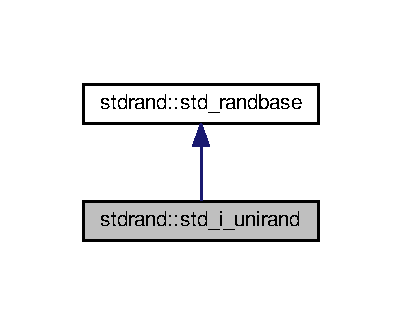
\includegraphics[width=193pt]{d5/d96/classstdrand_1_1std__i__unirand__inherit__graph}
\end{center}
\end{figure}


Collaboration diagram for stdrand\+:\+:std\+\_\+i\+\_\+unirand\+:
\nopagebreak
\begin{figure}[H]
\begin{center}
\leavevmode
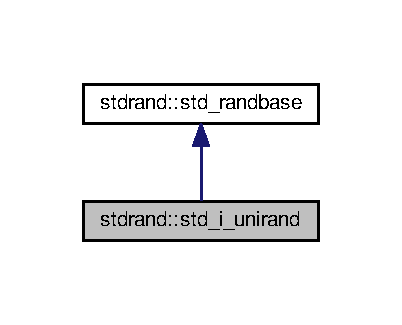
\includegraphics[width=193pt]{d1/d98/classstdrand_1_1std__i__unirand__coll__graph}
\end{center}
\end{figure}
\subsection*{Public Member Functions}
\begin{DoxyCompactItemize}
\item 
\hyperlink{classstdrand_1_1std__i__unirand_a3b8eb8ad27965c98c11d0e62f2f267d6}{std\+\_\+i\+\_\+unirand} (int seed)
\begin{DoxyCompactList}\small\item\em Constructor. \end{DoxyCompactList}\item 
\hyperlink{classstdrand_1_1std__i__unirand_aa43afdb4002553c1d03232e67733de75}{std\+\_\+i\+\_\+unirand} (int size, int seed)
\begin{DoxyCompactList}\small\item\em Constructor with dummy size input. \end{DoxyCompactList}\item 
\hyperlink{classstdrand_1_1std__i__unirand_a1e5b98aecea36f642c829ed5f4e452fc}{$\sim$std\+\_\+i\+\_\+unirand} ()
\begin{DoxyCompactList}\small\item\em Default destructor. \end{DoxyCompactList}\item 
double \hyperlink{classstdrand_1_1std__i__unirand_abe9833ea9fab736cf3b03b529498b767}{gen} ()
\begin{DoxyCompactList}\small\item\em Return a single random number. \end{DoxyCompactList}\end{DoxyCompactItemize}
\subsection*{Additional Inherited Members}


\subsection{Detailed Description}
Generator for uniform integers between 0 and 1. 

\subsection{Constructor \& Destructor Documentation}
\index{stdrand\+::std\+\_\+i\+\_\+unirand@{stdrand\+::std\+\_\+i\+\_\+unirand}!std\+\_\+i\+\_\+unirand@{std\+\_\+i\+\_\+unirand}}
\index{std\+\_\+i\+\_\+unirand@{std\+\_\+i\+\_\+unirand}!stdrand\+::std\+\_\+i\+\_\+unirand@{stdrand\+::std\+\_\+i\+\_\+unirand}}
\subsubsection[{\texorpdfstring{std\+\_\+i\+\_\+unirand(int seed)}{std_i_unirand(int seed)}}]{\setlength{\rightskip}{0pt plus 5cm}stdrand\+::std\+\_\+i\+\_\+unirand\+::std\+\_\+i\+\_\+unirand (
\begin{DoxyParamCaption}
\item[{int}]{seed}
\end{DoxyParamCaption}
)}\hypertarget{classstdrand_1_1std__i__unirand_a3b8eb8ad27965c98c11d0e62f2f267d6}{}\label{classstdrand_1_1std__i__unirand_a3b8eb8ad27965c98c11d0e62f2f267d6}


Constructor. 


\begin{DoxyParams}{Parameters}
{\em seed} & The inital seed of the random number generator. \\
\hline
\end{DoxyParams}
\index{stdrand\+::std\+\_\+i\+\_\+unirand@{stdrand\+::std\+\_\+i\+\_\+unirand}!std\+\_\+i\+\_\+unirand@{std\+\_\+i\+\_\+unirand}}
\index{std\+\_\+i\+\_\+unirand@{std\+\_\+i\+\_\+unirand}!stdrand\+::std\+\_\+i\+\_\+unirand@{stdrand\+::std\+\_\+i\+\_\+unirand}}
\subsubsection[{\texorpdfstring{std\+\_\+i\+\_\+unirand(int size, int seed)}{std_i_unirand(int size, int seed)}}]{\setlength{\rightskip}{0pt plus 5cm}stdrand\+::std\+\_\+i\+\_\+unirand\+::std\+\_\+i\+\_\+unirand (
\begin{DoxyParamCaption}
\item[{int}]{size, }
\item[{int}]{seed}
\end{DoxyParamCaption}
)\hspace{0.3cm}{\ttfamily [inline]}}\hypertarget{classstdrand_1_1std__i__unirand_aa43afdb4002553c1d03232e67733de75}{}\label{classstdrand_1_1std__i__unirand_aa43afdb4002553c1d03232e67733de75}


Constructor with dummy size input. 


\begin{DoxyParams}{Parameters}
{\em seed} & The inital seed of the random number generator. \\
\hline
{\em size} & A dummy size input for compatibility with Intel R\+NG. \\
\hline
\end{DoxyParams}
\index{stdrand\+::std\+\_\+i\+\_\+unirand@{stdrand\+::std\+\_\+i\+\_\+unirand}!````~std\+\_\+i\+\_\+unirand@{$\sim$std\+\_\+i\+\_\+unirand}}
\index{````~std\+\_\+i\+\_\+unirand@{$\sim$std\+\_\+i\+\_\+unirand}!stdrand\+::std\+\_\+i\+\_\+unirand@{stdrand\+::std\+\_\+i\+\_\+unirand}}
\subsubsection[{\texorpdfstring{$\sim$std\+\_\+i\+\_\+unirand()}{~std_i_unirand()}}]{\setlength{\rightskip}{0pt plus 5cm}stdrand\+::std\+\_\+i\+\_\+unirand\+::$\sim$std\+\_\+i\+\_\+unirand (
\begin{DoxyParamCaption}
{}
\end{DoxyParamCaption}
)\hspace{0.3cm}{\ttfamily [inline]}}\hypertarget{classstdrand_1_1std__i__unirand_a1e5b98aecea36f642c829ed5f4e452fc}{}\label{classstdrand_1_1std__i__unirand_a1e5b98aecea36f642c829ed5f4e452fc}


Default destructor. 



\subsection{Member Function Documentation}
\index{stdrand\+::std\+\_\+i\+\_\+unirand@{stdrand\+::std\+\_\+i\+\_\+unirand}!gen@{gen}}
\index{gen@{gen}!stdrand\+::std\+\_\+i\+\_\+unirand@{stdrand\+::std\+\_\+i\+\_\+unirand}}
\subsubsection[{\texorpdfstring{gen()}{gen()}}]{\setlength{\rightskip}{0pt plus 5cm}double stdrand\+::std\+\_\+i\+\_\+unirand\+::gen (
\begin{DoxyParamCaption}
{}
\end{DoxyParamCaption}
)\hspace{0.3cm}{\ttfamily [inline]}}\hypertarget{classstdrand_1_1std__i__unirand_abe9833ea9fab736cf3b03b529498b767}{}\label{classstdrand_1_1std__i__unirand_abe9833ea9fab736cf3b03b529498b767}


Return a single random number. 



The documentation for this class was generated from the following file\+:\begin{DoxyCompactItemize}
\item 
includes/\hyperlink{stdrand_8hpp}{stdrand.\+hpp}\end{DoxyCompactItemize}

\hypertarget{classstdrand_1_1std__lognormrand}{}\section{stdrand\+:\+:std\+\_\+lognormrand Class Reference}
\label{classstdrand_1_1std__lognormrand}\index{stdrand\+::std\+\_\+lognormrand@{stdrand\+::std\+\_\+lognormrand}}


Generator for random numbers on a normal distribution.  




{\ttfamily \#include $<$stdrand.\+hpp$>$}



Inheritance diagram for stdrand\+:\+:std\+\_\+lognormrand\+:
\nopagebreak
\begin{figure}[H]
\begin{center}
\leavevmode
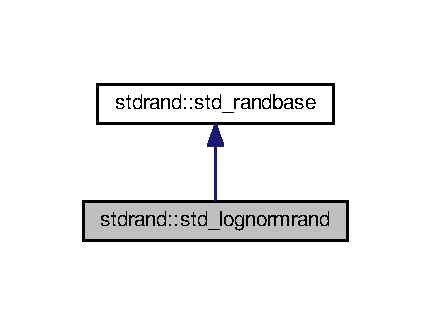
\includegraphics[width=207pt]{d2/deb/classstdrand_1_1std__lognormrand__inherit__graph}
\end{center}
\end{figure}


Collaboration diagram for stdrand\+:\+:std\+\_\+lognormrand\+:
\nopagebreak
\begin{figure}[H]
\begin{center}
\leavevmode
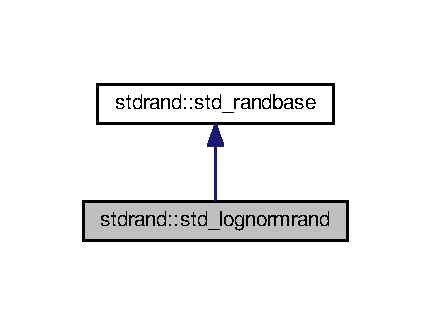
\includegraphics[width=207pt]{d1/d02/classstdrand_1_1std__lognormrand__coll__graph}
\end{center}
\end{figure}
\subsection*{Public Member Functions}
\begin{DoxyCompactItemize}
\item 
\hyperlink{classstdrand_1_1std__lognormrand_a4d27599458dc5b075d723a445431d2f7}{std\+\_\+lognormrand} (double m, double sdin, int seed)
\begin{DoxyCompactList}\small\item\em Constructor. \end{DoxyCompactList}\item 
\hyperlink{classstdrand_1_1std__lognormrand_a21729248c87a39d6522a405a85b6a808}{std\+\_\+lognormrand} (double m, double sdin, int size, int seed)
\begin{DoxyCompactList}\small\item\em Constructor with dummy size. \end{DoxyCompactList}\item 
\hyperlink{classstdrand_1_1std__lognormrand_af73b651b8fde69e3535660eca7fac95f}{$\sim$std\+\_\+lognormrand} ()
\begin{DoxyCompactList}\small\item\em Default destructor. \end{DoxyCompactList}\item 
double \hyperlink{classstdrand_1_1std__lognormrand_a4521bea46b321ea53a2026eac8dc046a}{gen} ()
\begin{DoxyCompactList}\small\item\em Return a single random number. \end{DoxyCompactList}\end{DoxyCompactItemize}
\subsection*{Additional Inherited Members}


\subsection{Detailed Description}
Generator for random numbers on a normal distribution. 

\subsection{Constructor \& Destructor Documentation}
\index{stdrand\+::std\+\_\+lognormrand@{stdrand\+::std\+\_\+lognormrand}!std\+\_\+lognormrand@{std\+\_\+lognormrand}}
\index{std\+\_\+lognormrand@{std\+\_\+lognormrand}!stdrand\+::std\+\_\+lognormrand@{stdrand\+::std\+\_\+lognormrand}}
\subsubsection[{\texorpdfstring{std\+\_\+lognormrand(double m, double sdin, int seed)}{std_lognormrand(double m, double sdin, int seed)}}]{\setlength{\rightskip}{0pt plus 5cm}stdrand\+::std\+\_\+lognormrand\+::std\+\_\+lognormrand (
\begin{DoxyParamCaption}
\item[{double}]{m, }
\item[{double}]{sdin, }
\item[{int}]{seed}
\end{DoxyParamCaption}
)}\hypertarget{classstdrand_1_1std__lognormrand_a4d27599458dc5b075d723a445431d2f7}{}\label{classstdrand_1_1std__lognormrand_a4d27599458dc5b075d723a445431d2f7}


Constructor. 


\begin{DoxyParams}{Parameters}
{\em m} & The logarithmic mean of the lognormal distribution. \\
\hline
{\em sdin} & The logarithmic standard deviation of the lognormal distribution. \\
\hline
{\em seed} & The inital seed of the random number generator. \\
\hline
\end{DoxyParams}
\index{stdrand\+::std\+\_\+lognormrand@{stdrand\+::std\+\_\+lognormrand}!std\+\_\+lognormrand@{std\+\_\+lognormrand}}
\index{std\+\_\+lognormrand@{std\+\_\+lognormrand}!stdrand\+::std\+\_\+lognormrand@{stdrand\+::std\+\_\+lognormrand}}
\subsubsection[{\texorpdfstring{std\+\_\+lognormrand(double m, double sdin, int size, int seed)}{std_lognormrand(double m, double sdin, int size, int seed)}}]{\setlength{\rightskip}{0pt plus 5cm}stdrand\+::std\+\_\+lognormrand\+::std\+\_\+lognormrand (
\begin{DoxyParamCaption}
\item[{double}]{m, }
\item[{double}]{sdin, }
\item[{int}]{size, }
\item[{int}]{seed}
\end{DoxyParamCaption}
)\hspace{0.3cm}{\ttfamily [inline]}}\hypertarget{classstdrand_1_1std__lognormrand_a21729248c87a39d6522a405a85b6a808}{}\label{classstdrand_1_1std__lognormrand_a21729248c87a39d6522a405a85b6a808}


Constructor with dummy size. 


\begin{DoxyParams}{Parameters}
{\em m} & The logarithmic mean of the lognormal distribution. \\
\hline
{\em sdin} & The logarithmic standard deviation of the lognormal distribution. \\
\hline
{\em seed} & The inital seed of the random number generator. \\
\hline
{\em size} & A dummy size input for compatibility with Intel R\+NG. \\
\hline
\end{DoxyParams}
\index{stdrand\+::std\+\_\+lognormrand@{stdrand\+::std\+\_\+lognormrand}!````~std\+\_\+lognormrand@{$\sim$std\+\_\+lognormrand}}
\index{````~std\+\_\+lognormrand@{$\sim$std\+\_\+lognormrand}!stdrand\+::std\+\_\+lognormrand@{stdrand\+::std\+\_\+lognormrand}}
\subsubsection[{\texorpdfstring{$\sim$std\+\_\+lognormrand()}{~std_lognormrand()}}]{\setlength{\rightskip}{0pt plus 5cm}stdrand\+::std\+\_\+lognormrand\+::$\sim$std\+\_\+lognormrand (
\begin{DoxyParamCaption}
{}
\end{DoxyParamCaption}
)\hspace{0.3cm}{\ttfamily [inline]}}\hypertarget{classstdrand_1_1std__lognormrand_af73b651b8fde69e3535660eca7fac95f}{}\label{classstdrand_1_1std__lognormrand_af73b651b8fde69e3535660eca7fac95f}


Default destructor. 



\subsection{Member Function Documentation}
\index{stdrand\+::std\+\_\+lognormrand@{stdrand\+::std\+\_\+lognormrand}!gen@{gen}}
\index{gen@{gen}!stdrand\+::std\+\_\+lognormrand@{stdrand\+::std\+\_\+lognormrand}}
\subsubsection[{\texorpdfstring{gen()}{gen()}}]{\setlength{\rightskip}{0pt plus 5cm}double stdrand\+::std\+\_\+lognormrand\+::gen (
\begin{DoxyParamCaption}
{}
\end{DoxyParamCaption}
)\hspace{0.3cm}{\ttfamily [inline]}}\hypertarget{classstdrand_1_1std__lognormrand_a4521bea46b321ea53a2026eac8dc046a}{}\label{classstdrand_1_1std__lognormrand_a4521bea46b321ea53a2026eac8dc046a}


Return a single random number. 



The documentation for this class was generated from the following file\+:\begin{DoxyCompactItemize}
\item 
includes/\hyperlink{stdrand_8hpp}{stdrand.\+hpp}\end{DoxyCompactItemize}

\hypertarget{classstdrand_1_1std__normrand}{}\section{stdrand\+:\+:std\+\_\+normrand Class Reference}
\label{classstdrand_1_1std__normrand}\index{stdrand\+::std\+\_\+normrand@{stdrand\+::std\+\_\+normrand}}


Generator for random numbers on a normal distribution.  




{\ttfamily \#include $<$stdrand.\+hpp$>$}



Inheritance diagram for stdrand\+:\+:std\+\_\+normrand\+:
\nopagebreak
\begin{figure}[H]
\begin{center}
\leavevmode
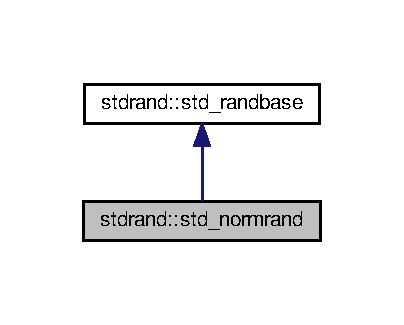
\includegraphics[width=194pt]{d0/df7/classstdrand_1_1std__normrand__inherit__graph}
\end{center}
\end{figure}


Collaboration diagram for stdrand\+:\+:std\+\_\+normrand\+:
\nopagebreak
\begin{figure}[H]
\begin{center}
\leavevmode
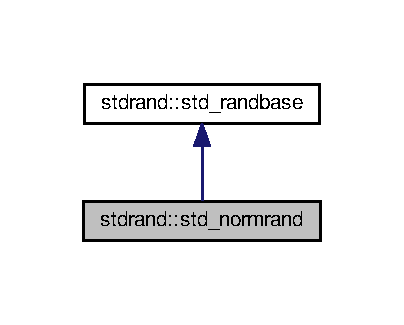
\includegraphics[width=194pt]{d6/d3d/classstdrand_1_1std__normrand__coll__graph}
\end{center}
\end{figure}
\subsection*{Public Member Functions}
\begin{DoxyCompactItemize}
\item 
\hyperlink{classstdrand_1_1std__normrand_a2cb06e8547d4475a424d213cda700ad7}{std\+\_\+normrand} (double m, double sdin, int seed=1)
\begin{DoxyCompactList}\small\item\em Constructor. \end{DoxyCompactList}\item 
\hyperlink{classstdrand_1_1std__normrand_aec1727d2023b6acc65a4057a71ee642a}{$\sim$std\+\_\+normrand} ()
\begin{DoxyCompactList}\small\item\em Default destructor. \end{DoxyCompactList}\item 
double \hyperlink{classstdrand_1_1std__normrand_adf3d7e53ddd7a0aa6b43b08038f09c91}{gen} ()
\begin{DoxyCompactList}\small\item\em Return a single random number. \end{DoxyCompactList}\end{DoxyCompactItemize}
\subsection*{Additional Inherited Members}


\subsection{Detailed Description}
Generator for random numbers on a normal distribution. 

\subsection{Constructor \& Destructor Documentation}
\index{stdrand\+::std\+\_\+normrand@{stdrand\+::std\+\_\+normrand}!std\+\_\+normrand@{std\+\_\+normrand}}
\index{std\+\_\+normrand@{std\+\_\+normrand}!stdrand\+::std\+\_\+normrand@{stdrand\+::std\+\_\+normrand}}
\subsubsection[{\texorpdfstring{std\+\_\+normrand(double m, double sdin, int seed=1)}{std_normrand(double m, double sdin, int seed=1)}}]{\setlength{\rightskip}{0pt plus 5cm}stdrand\+::std\+\_\+normrand\+::std\+\_\+normrand (
\begin{DoxyParamCaption}
\item[{double}]{m, }
\item[{double}]{sdin, }
\item[{int}]{seed = {\ttfamily 1}}
\end{DoxyParamCaption}
)}\hypertarget{classstdrand_1_1std__normrand_a2cb06e8547d4475a424d213cda700ad7}{}\label{classstdrand_1_1std__normrand_a2cb06e8547d4475a424d213cda700ad7}


Constructor. 


\begin{DoxyParams}{Parameters}
{\em m} & The mean of the normal distribution. \\
\hline
{\em sdin} & The standard deviation of the normal distribution. \\
\hline
{\em seed} & The inital seed of the random number generator. Defaults to 1. \\
\hline
\end{DoxyParams}
\index{stdrand\+::std\+\_\+normrand@{stdrand\+::std\+\_\+normrand}!````~std\+\_\+normrand@{$\sim$std\+\_\+normrand}}
\index{````~std\+\_\+normrand@{$\sim$std\+\_\+normrand}!stdrand\+::std\+\_\+normrand@{stdrand\+::std\+\_\+normrand}}
\subsubsection[{\texorpdfstring{$\sim$std\+\_\+normrand()}{~std_normrand()}}]{\setlength{\rightskip}{0pt plus 5cm}stdrand\+::std\+\_\+normrand\+::$\sim$std\+\_\+normrand (
\begin{DoxyParamCaption}
{}
\end{DoxyParamCaption}
)\hspace{0.3cm}{\ttfamily [inline]}}\hypertarget{classstdrand_1_1std__normrand_aec1727d2023b6acc65a4057a71ee642a}{}\label{classstdrand_1_1std__normrand_aec1727d2023b6acc65a4057a71ee642a}


Default destructor. 



\subsection{Member Function Documentation}
\index{stdrand\+::std\+\_\+normrand@{stdrand\+::std\+\_\+normrand}!gen@{gen}}
\index{gen@{gen}!stdrand\+::std\+\_\+normrand@{stdrand\+::std\+\_\+normrand}}
\subsubsection[{\texorpdfstring{gen()}{gen()}}]{\setlength{\rightskip}{0pt plus 5cm}double stdrand\+::std\+\_\+normrand\+::gen (
\begin{DoxyParamCaption}
{}
\end{DoxyParamCaption}
)\hspace{0.3cm}{\ttfamily [inline]}}\hypertarget{classstdrand_1_1std__normrand_adf3d7e53ddd7a0aa6b43b08038f09c91}{}\label{classstdrand_1_1std__normrand_adf3d7e53ddd7a0aa6b43b08038f09c91}


Return a single random number. 



The documentation for this class was generated from the following file\+:\begin{DoxyCompactItemize}
\item 
includes/\hyperlink{stdrand_8hpp}{stdrand.\+hpp}\end{DoxyCompactItemize}

\hypertarget{classstdrand_1_1std__randbase}{}\section{stdrand\+:\+:std\+\_\+randbase Class Reference}
\label{classstdrand_1_1std__randbase}\index{stdrand\+::std\+\_\+randbase@{stdrand\+::std\+\_\+randbase}}


Base class for the random number generators.  




{\ttfamily \#include $<$stdrand.\+hpp$>$}



Inheritance diagram for stdrand\+:\+:std\+\_\+randbase\+:\nopagebreak
\begin{figure}[H]
\begin{center}
\leavevmode
\includegraphics[width=350pt]{d1/d27/classstdrand_1_1std__randbase__inherit__graph}
\end{center}
\end{figure}


Collaboration diagram for stdrand\+:\+:std\+\_\+randbase\+:
\nopagebreak
\begin{figure}[H]
\begin{center}
\leavevmode
\includegraphics[width=193pt]{d0/d37/classstdrand_1_1std__randbase__coll__graph}
\end{center}
\end{figure}
\subsection*{Public Member Functions}
\begin{DoxyCompactItemize}
\item 
\hyperlink{classstdrand_1_1std__randbase_a8298d43186d6410f30ec0a77f0b90159}{std\+\_\+randbase} ()
\begin{DoxyCompactList}\small\item\em Default constructor. \end{DoxyCompactList}\item 
\hyperlink{classstdrand_1_1std__randbase_a5280080005689ab2ff6dae6de10a3faa}{$\sim$std\+\_\+randbase} ()
\begin{DoxyCompactList}\small\item\em Default destructor. \end{DoxyCompactList}\item 
void \hyperlink{classstdrand_1_1std__randbase_ae4d2a7ab5253b8d21ce4ede8f9988f24}{change\+\_\+seed} (int seed)
\begin{DoxyCompactList}\small\item\em Change the current random seed. \end{DoxyCompactList}\item 
void \hyperlink{classstdrand_1_1std__randbase_a1f59d641467d33c51df65651212dac1f}{jump} ()
\begin{DoxyCompactList}\small\item\em Jump forward 2$^\wedge$64 places. \end{DoxyCompactList}\end{DoxyCompactItemize}
\subsection*{Protected Attributes}
\begin{DoxyCompactItemize}
\item 
\hyperlink{structrng_1_1rng128}{rng\+::rng128} \hyperlink{classstdrand_1_1std__randbase_a04dc8f49595791e10967b74a4b137b53}{generator}
\end{DoxyCompactItemize}


\subsection{Detailed Description}
Base class for the random number generators. 

\subsection{Constructor \& Destructor Documentation}
\index{stdrand\+::std\+\_\+randbase@{stdrand\+::std\+\_\+randbase}!std\+\_\+randbase@{std\+\_\+randbase}}
\index{std\+\_\+randbase@{std\+\_\+randbase}!stdrand\+::std\+\_\+randbase@{stdrand\+::std\+\_\+randbase}}
\subsubsection[{\texorpdfstring{std\+\_\+randbase()}{std_randbase()}}]{\setlength{\rightskip}{0pt plus 5cm}stdrand\+::std\+\_\+randbase\+::std\+\_\+randbase (
\begin{DoxyParamCaption}
{}
\end{DoxyParamCaption}
)\hspace{0.3cm}{\ttfamily [inline]}}\hypertarget{classstdrand_1_1std__randbase_a8298d43186d6410f30ec0a77f0b90159}{}\label{classstdrand_1_1std__randbase_a8298d43186d6410f30ec0a77f0b90159}


Default constructor. 

\index{stdrand\+::std\+\_\+randbase@{stdrand\+::std\+\_\+randbase}!````~std\+\_\+randbase@{$\sim$std\+\_\+randbase}}
\index{````~std\+\_\+randbase@{$\sim$std\+\_\+randbase}!stdrand\+::std\+\_\+randbase@{stdrand\+::std\+\_\+randbase}}
\subsubsection[{\texorpdfstring{$\sim$std\+\_\+randbase()}{~std_randbase()}}]{\setlength{\rightskip}{0pt plus 5cm}stdrand\+::std\+\_\+randbase\+::$\sim$std\+\_\+randbase (
\begin{DoxyParamCaption}
{}
\end{DoxyParamCaption}
)\hspace{0.3cm}{\ttfamily [inline]}}\hypertarget{classstdrand_1_1std__randbase_a5280080005689ab2ff6dae6de10a3faa}{}\label{classstdrand_1_1std__randbase_a5280080005689ab2ff6dae6de10a3faa}


Default destructor. 



\subsection{Member Function Documentation}
\index{stdrand\+::std\+\_\+randbase@{stdrand\+::std\+\_\+randbase}!change\+\_\+seed@{change\+\_\+seed}}
\index{change\+\_\+seed@{change\+\_\+seed}!stdrand\+::std\+\_\+randbase@{stdrand\+::std\+\_\+randbase}}
\subsubsection[{\texorpdfstring{change\+\_\+seed(int seed)}{change_seed(int seed)}}]{\setlength{\rightskip}{0pt plus 5cm}void stdrand\+::std\+\_\+randbase\+::change\+\_\+seed (
\begin{DoxyParamCaption}
\item[{int}]{seed}
\end{DoxyParamCaption}
)\hspace{0.3cm}{\ttfamily [inline]}}\hypertarget{classstdrand_1_1std__randbase_ae4d2a7ab5253b8d21ce4ede8f9988f24}{}\label{classstdrand_1_1std__randbase_ae4d2a7ab5253b8d21ce4ede8f9988f24}


Change the current random seed. 


\begin{DoxyParams}{Parameters}
{\em seed} & The new seed. \\
\hline
\end{DoxyParams}
\index{stdrand\+::std\+\_\+randbase@{stdrand\+::std\+\_\+randbase}!jump@{jump}}
\index{jump@{jump}!stdrand\+::std\+\_\+randbase@{stdrand\+::std\+\_\+randbase}}
\subsubsection[{\texorpdfstring{jump()}{jump()}}]{\setlength{\rightskip}{0pt plus 5cm}void stdrand\+::std\+\_\+randbase\+::jump (
\begin{DoxyParamCaption}
{}
\end{DoxyParamCaption}
)\hspace{0.3cm}{\ttfamily [inline]}}\hypertarget{classstdrand_1_1std__randbase_a1f59d641467d33c51df65651212dac1f}{}\label{classstdrand_1_1std__randbase_a1f59d641467d33c51df65651212dac1f}


Jump forward 2$^\wedge$64 places. 



\subsection{Member Data Documentation}
\index{stdrand\+::std\+\_\+randbase@{stdrand\+::std\+\_\+randbase}!generator@{generator}}
\index{generator@{generator}!stdrand\+::std\+\_\+randbase@{stdrand\+::std\+\_\+randbase}}
\subsubsection[{\texorpdfstring{generator}{generator}}]{\setlength{\rightskip}{0pt plus 5cm}{\bf rng\+::rng128} stdrand\+::std\+\_\+randbase\+::generator\hspace{0.3cm}{\ttfamily [protected]}}\hypertarget{classstdrand_1_1std__randbase_a04dc8f49595791e10967b74a4b137b53}{}\label{classstdrand_1_1std__randbase_a04dc8f49595791e10967b74a4b137b53}


The documentation for this class was generated from the following file\+:\begin{DoxyCompactItemize}
\item 
includes/\hyperlink{stdrand_8hpp}{stdrand.\+hpp}\end{DoxyCompactItemize}

\hypertarget{classparticle_1_1shape_1_1weibull}{}\section{particle\+:\+:shape\+:\+:weibull Class Reference}
\label{classparticle_1_1shape_1_1weibull}\index{particle\+::shape\+::weibull@{particle\+::shape\+::weibull}}


Weibull disordered circle/sphere particle.  




{\ttfamily \#include $<$shape.\+hpp$>$}



Inheritance diagram for particle\+:\+:shape\+:\+:weibull\+:\nopagebreak
\begin{figure}[H]
\begin{center}
\leavevmode
\includegraphics[width=217pt]{dc/d64/classparticle_1_1shape_1_1weibull__inherit__graph}
\end{center}
\end{figure}


Collaboration diagram for particle\+:\+:shape\+:\+:weibull\+:\nopagebreak
\begin{figure}[H]
\begin{center}
\leavevmode
\includegraphics[width=217pt]{dd/d57/classparticle_1_1shape_1_1weibull__coll__graph}
\end{center}
\end{figure}
\subsection*{Public Member Functions}
\begin{DoxyCompactItemize}
\item 
\hyperlink{classparticle_1_1shape_1_1weibull_a6171e8485c445df5322b61bc4bd4d360}{weibull} ()
\begin{DoxyCompactList}\small\item\em Default constructor. \end{DoxyCompactList}\item 
\hyperlink{classparticle_1_1shape_1_1weibull_a4a30c2bc444fddc10e53331693b1b696}{weibull} (\hyperlink{classparticle_1_1shape_1_1shape__type}{shape\+\_\+type} \&other)
\begin{DoxyCompactList}\small\item\em Copy constructor. \end{DoxyCompactList}\item 
\hyperlink{classparticle_1_1shape_1_1weibull_ae3ea5c72d6cb62ba72308ed831bbc82d}{weibull} (double rin, double bin)
\begin{DoxyCompactList}\small\item\em Constructor defining a spherical particle with a disordered surface. \end{DoxyCompactList}\item 
\hyperlink{classparticle_1_1shape_1_1weibull_a63137884cacc8ab5df125ba862f79262}{weibull} (double betain, double ain, double bin, double cin)
\begin{DoxyCompactList}\small\item\em Constructor defining an ellipsoid particle with a disordered surface. \end{DoxyCompactList}\item 
\hyperlink{classparticle_1_1shape_1_1weibull_a02613f15cab64462293ff787c35fafb1}{$\sim$weibull} ()
\begin{DoxyCompactList}\small\item\em Default destructor. \end{DoxyCompactList}\item 
bool \hyperlink{classparticle_1_1shape_1_1weibull_a22612311ce2f3ca4317f8263e52de425}{check} (std\+::vector$<$ int $>$ Is, int l\+\_\+size)
\begin{DoxyCompactList}\small\item\em Check whether a certain position falls within the particle. \end{DoxyCompactList}\item 
\hyperlink{classparticle_1_1shape_1_1weibull}{weibull} \& \hyperlink{classparticle_1_1shape_1_1weibull_a682194c48696724e2290373b8c35577a}{operator=} (\hyperlink{classparticle_1_1shape_1_1shape__type}{shape\+\_\+type} \&other)
\begin{DoxyCompactList}\small\item\em Assignment operator. \end{DoxyCompactList}\item 
double \hyperlink{classparticle_1_1shape_1_1weibull_a85ab45f804ae9aa3fb712c435125ff70}{get\+\_\+r0} ()
\begin{DoxyCompactList}\small\item\em Returns the characteristic size of a weibull particle. \end{DoxyCompactList}\item 
double \hyperlink{classparticle_1_1shape_1_1weibull_a640180ce2bd6ce7f68c10d4791bce49c}{get\+\_\+beta} ()
\begin{DoxyCompactList}\small\item\em Returns the disorder parameter of a weibull particle. \end{DoxyCompactList}\item 
double \hyperlink{classparticle_1_1shape_1_1weibull_a0234fa42b67465c7191248f524f27a0e}{get\+\_\+a} ()
\begin{DoxyCompactList}\small\item\em Returns the x-\/axis radius of a weibull particle. \end{DoxyCompactList}\item 
double \hyperlink{classparticle_1_1shape_1_1weibull_a1066adcab828f8636475128ff51c56f0}{get\+\_\+b} ()
\begin{DoxyCompactList}\small\item\em Returns the y-\/axis radius of a weibull particle. \end{DoxyCompactList}\item 
double \hyperlink{classparticle_1_1shape_1_1weibull_a0b8c38944e502df7bce4e8f99d149237}{get\+\_\+c} ()
\begin{DoxyCompactList}\small\item\em Returns the z-\/axis radius of a weibull particle. \end{DoxyCompactList}\end{DoxyCompactItemize}


\subsection{Detailed Description}
Weibull disordered circle/sphere particle. 

\subsection{Constructor \& Destructor Documentation}
\index{particle\+::shape\+::weibull@{particle\+::shape\+::weibull}!weibull@{weibull}}
\index{weibull@{weibull}!particle\+::shape\+::weibull@{particle\+::shape\+::weibull}}
\subsubsection[{\texorpdfstring{weibull()}{weibull()}}]{\setlength{\rightskip}{0pt plus 5cm}particle\+::shape\+::weibull\+::weibull (
\begin{DoxyParamCaption}
{}
\end{DoxyParamCaption}
)\hspace{0.3cm}{\ttfamily [inline]}}\hypertarget{classparticle_1_1shape_1_1weibull_a6171e8485c445df5322b61bc4bd4d360}{}\label{classparticle_1_1shape_1_1weibull_a6171e8485c445df5322b61bc4bd4d360}


Default constructor. 

\index{particle\+::shape\+::weibull@{particle\+::shape\+::weibull}!weibull@{weibull}}
\index{weibull@{weibull}!particle\+::shape\+::weibull@{particle\+::shape\+::weibull}}
\subsubsection[{\texorpdfstring{weibull(shape\+\_\+type \&other)}{weibull(shape_type &other)}}]{\setlength{\rightskip}{0pt plus 5cm}particle\+::shape\+::weibull\+::weibull (
\begin{DoxyParamCaption}
\item[{{\bf shape\+\_\+type} \&}]{other}
\end{DoxyParamCaption}
)}\hypertarget{classparticle_1_1shape_1_1weibull_a4a30c2bc444fddc10e53331693b1b696}{}\label{classparticle_1_1shape_1_1weibull_a4a30c2bc444fddc10e53331693b1b696}


Copy constructor. 

\index{particle\+::shape\+::weibull@{particle\+::shape\+::weibull}!weibull@{weibull}}
\index{weibull@{weibull}!particle\+::shape\+::weibull@{particle\+::shape\+::weibull}}
\subsubsection[{\texorpdfstring{weibull(double rin, double bin)}{weibull(double rin, double bin)}}]{\setlength{\rightskip}{0pt plus 5cm}particle\+::shape\+::weibull\+::weibull (
\begin{DoxyParamCaption}
\item[{double}]{rin, }
\item[{double}]{bin}
\end{DoxyParamCaption}
)}\hypertarget{classparticle_1_1shape_1_1weibull_ae3ea5c72d6cb62ba72308ed831bbc82d}{}\label{classparticle_1_1shape_1_1weibull_ae3ea5c72d6cb62ba72308ed831bbc82d}


Constructor defining a spherical particle with a disordered surface. 


\begin{DoxyParams}{Parameters}
{\em rin} & The average radius of the sphere. \\
\hline
{\em bin} & The disorder parameter. \\
\hline
\end{DoxyParams}
\index{particle\+::shape\+::weibull@{particle\+::shape\+::weibull}!weibull@{weibull}}
\index{weibull@{weibull}!particle\+::shape\+::weibull@{particle\+::shape\+::weibull}}
\subsubsection[{\texorpdfstring{weibull(double betain, double ain, double bin, double cin)}{weibull(double betain, double ain, double bin, double cin)}}]{\setlength{\rightskip}{0pt plus 5cm}particle\+::shape\+::weibull\+::weibull (
\begin{DoxyParamCaption}
\item[{double}]{betain, }
\item[{double}]{ain, }
\item[{double}]{bin, }
\item[{double}]{cin}
\end{DoxyParamCaption}
)}\hypertarget{classparticle_1_1shape_1_1weibull_a63137884cacc8ab5df125ba862f79262}{}\label{classparticle_1_1shape_1_1weibull_a63137884cacc8ab5df125ba862f79262}


Constructor defining an ellipsoid particle with a disordered surface. 


\begin{DoxyParams}{Parameters}
{\em betain} & The disorder parameter. \\
\hline
{\em ain} & The x-\/axis size of the particle. \\
\hline
{\em bin} & The y-\/axis size of the particle. \\
\hline
{\em cin} & The z-\/axis size of the particle. \\
\hline
\end{DoxyParams}
\index{particle\+::shape\+::weibull@{particle\+::shape\+::weibull}!````~weibull@{$\sim$weibull}}
\index{````~weibull@{$\sim$weibull}!particle\+::shape\+::weibull@{particle\+::shape\+::weibull}}
\subsubsection[{\texorpdfstring{$\sim$weibull()}{~weibull()}}]{\setlength{\rightskip}{0pt plus 5cm}particle\+::shape\+::weibull\+::$\sim$weibull (
\begin{DoxyParamCaption}
{}
\end{DoxyParamCaption}
)\hspace{0.3cm}{\ttfamily [inline]}}\hypertarget{classparticle_1_1shape_1_1weibull_a02613f15cab64462293ff787c35fafb1}{}\label{classparticle_1_1shape_1_1weibull_a02613f15cab64462293ff787c35fafb1}


Default destructor. 



\subsection{Member Function Documentation}
\index{particle\+::shape\+::weibull@{particle\+::shape\+::weibull}!check@{check}}
\index{check@{check}!particle\+::shape\+::weibull@{particle\+::shape\+::weibull}}
\subsubsection[{\texorpdfstring{check(std\+::vector$<$ int $>$ Is, int l\+\_\+size)}{check(std::vector< int > Is, int l_size)}}]{\setlength{\rightskip}{0pt plus 5cm}bool particle\+::shape\+::weibull\+::check (
\begin{DoxyParamCaption}
\item[{std\+::vector$<$ int $>$}]{Is, }
\item[{int}]{l\+\_\+size}
\end{DoxyParamCaption}
)\hspace{0.3cm}{\ttfamily [virtual]}}\hypertarget{classparticle_1_1shape_1_1weibull_a22612311ce2f3ca4317f8263e52de425}{}\label{classparticle_1_1shape_1_1weibull_a22612311ce2f3ca4317f8263e52de425}


Check whether a certain position falls within the particle. 


\begin{DoxyParams}{Parameters}
{\em Is} & The coordinates of the lattice site. \\
\hline
{\em l\+\_\+size} & The total lattice size. \\
\hline
\end{DoxyParams}


Reimplemented from \hyperlink{classparticle_1_1shape_1_1shape__type_a64d04f49c8da656d8b8899c431c346fc}{particle\+::shape\+::shape\+\_\+type}.

\index{particle\+::shape\+::weibull@{particle\+::shape\+::weibull}!get\+\_\+a@{get\+\_\+a}}
\index{get\+\_\+a@{get\+\_\+a}!particle\+::shape\+::weibull@{particle\+::shape\+::weibull}}
\subsubsection[{\texorpdfstring{get\+\_\+a()}{get_a()}}]{\setlength{\rightskip}{0pt plus 5cm}double particle\+::shape\+::weibull\+::get\+\_\+a (
\begin{DoxyParamCaption}
{}
\end{DoxyParamCaption}
)\hspace{0.3cm}{\ttfamily [inline]}, {\ttfamily [virtual]}}\hypertarget{classparticle_1_1shape_1_1weibull_a0234fa42b67465c7191248f524f27a0e}{}\label{classparticle_1_1shape_1_1weibull_a0234fa42b67465c7191248f524f27a0e}


Returns the x-\/axis radius of a weibull particle. 



Reimplemented from \hyperlink{classparticle_1_1shape_1_1shape__type_a7b938aa8c2dada71e8d0b11c6a676449}{particle\+::shape\+::shape\+\_\+type}.

\index{particle\+::shape\+::weibull@{particle\+::shape\+::weibull}!get\+\_\+b@{get\+\_\+b}}
\index{get\+\_\+b@{get\+\_\+b}!particle\+::shape\+::weibull@{particle\+::shape\+::weibull}}
\subsubsection[{\texorpdfstring{get\+\_\+b()}{get_b()}}]{\setlength{\rightskip}{0pt plus 5cm}double particle\+::shape\+::weibull\+::get\+\_\+b (
\begin{DoxyParamCaption}
{}
\end{DoxyParamCaption}
)\hspace{0.3cm}{\ttfamily [inline]}, {\ttfamily [virtual]}}\hypertarget{classparticle_1_1shape_1_1weibull_a1066adcab828f8636475128ff51c56f0}{}\label{classparticle_1_1shape_1_1weibull_a1066adcab828f8636475128ff51c56f0}


Returns the y-\/axis radius of a weibull particle. 



Reimplemented from \hyperlink{classparticle_1_1shape_1_1shape__type_a0a9f0a397edbc66120114c89a185c127}{particle\+::shape\+::shape\+\_\+type}.

\index{particle\+::shape\+::weibull@{particle\+::shape\+::weibull}!get\+\_\+beta@{get\+\_\+beta}}
\index{get\+\_\+beta@{get\+\_\+beta}!particle\+::shape\+::weibull@{particle\+::shape\+::weibull}}
\subsubsection[{\texorpdfstring{get\+\_\+beta()}{get_beta()}}]{\setlength{\rightskip}{0pt plus 5cm}double particle\+::shape\+::weibull\+::get\+\_\+beta (
\begin{DoxyParamCaption}
{}
\end{DoxyParamCaption}
)\hspace{0.3cm}{\ttfamily [inline]}, {\ttfamily [virtual]}}\hypertarget{classparticle_1_1shape_1_1weibull_a640180ce2bd6ce7f68c10d4791bce49c}{}\label{classparticle_1_1shape_1_1weibull_a640180ce2bd6ce7f68c10d4791bce49c}


Returns the disorder parameter of a weibull particle. 



Reimplemented from \hyperlink{classparticle_1_1shape_1_1shape__type_a041dd08774f26ffeeb051e1442cb612c}{particle\+::shape\+::shape\+\_\+type}.

\index{particle\+::shape\+::weibull@{particle\+::shape\+::weibull}!get\+\_\+c@{get\+\_\+c}}
\index{get\+\_\+c@{get\+\_\+c}!particle\+::shape\+::weibull@{particle\+::shape\+::weibull}}
\subsubsection[{\texorpdfstring{get\+\_\+c()}{get_c()}}]{\setlength{\rightskip}{0pt plus 5cm}double particle\+::shape\+::weibull\+::get\+\_\+c (
\begin{DoxyParamCaption}
{}
\end{DoxyParamCaption}
)\hspace{0.3cm}{\ttfamily [inline]}, {\ttfamily [virtual]}}\hypertarget{classparticle_1_1shape_1_1weibull_a0b8c38944e502df7bce4e8f99d149237}{}\label{classparticle_1_1shape_1_1weibull_a0b8c38944e502df7bce4e8f99d149237}


Returns the z-\/axis radius of a weibull particle. 



Reimplemented from \hyperlink{classparticle_1_1shape_1_1shape__type_a4f37d43b6e014a429e45480cea48f63d}{particle\+::shape\+::shape\+\_\+type}.

\index{particle\+::shape\+::weibull@{particle\+::shape\+::weibull}!get\+\_\+r0@{get\+\_\+r0}}
\index{get\+\_\+r0@{get\+\_\+r0}!particle\+::shape\+::weibull@{particle\+::shape\+::weibull}}
\subsubsection[{\texorpdfstring{get\+\_\+r0()}{get_r0()}}]{\setlength{\rightskip}{0pt plus 5cm}double particle\+::shape\+::weibull\+::get\+\_\+r0 (
\begin{DoxyParamCaption}
{}
\end{DoxyParamCaption}
)\hspace{0.3cm}{\ttfamily [inline]}, {\ttfamily [virtual]}}\hypertarget{classparticle_1_1shape_1_1weibull_a85ab45f804ae9aa3fb712c435125ff70}{}\label{classparticle_1_1shape_1_1weibull_a85ab45f804ae9aa3fb712c435125ff70}


Returns the characteristic size of a weibull particle. 



Reimplemented from \hyperlink{classparticle_1_1shape_1_1shape__type_a062dfaf9cbfe98cdcdc55c34a0463313}{particle\+::shape\+::shape\+\_\+type}.

\index{particle\+::shape\+::weibull@{particle\+::shape\+::weibull}!operator=@{operator=}}
\index{operator=@{operator=}!particle\+::shape\+::weibull@{particle\+::shape\+::weibull}}
\subsubsection[{\texorpdfstring{operator=(shape\+\_\+type \&other)}{operator=(shape_type &other)}}]{\setlength{\rightskip}{0pt plus 5cm}{\bf weibull}\& particle\+::shape\+::weibull\+::operator= (
\begin{DoxyParamCaption}
\item[{{\bf shape\+\_\+type} \&}]{other}
\end{DoxyParamCaption}
)}\hypertarget{classparticle_1_1shape_1_1weibull_a682194c48696724e2290373b8c35577a}{}\label{classparticle_1_1shape_1_1weibull_a682194c48696724e2290373b8c35577a}


Assignment operator. 



The documentation for this class was generated from the following file\+:\begin{DoxyCompactItemize}
\item 
includes/\hyperlink{shape_8hpp}{shape.\+hpp}\end{DoxyCompactItemize}

\chapter{File Documentation}
\hypertarget{array__alloc_8hpp}{}\section{includes/array\+\_\+alloc.hpp File Reference}
\label{array__alloc_8hpp}\index{includes/array\+\_\+alloc.\+hpp@{includes/array\+\_\+alloc.\+hpp}}
This graph shows which files directly or indirectly include this file\+:
\nopagebreak
\begin{figure}[H]
\begin{center}
\leavevmode
\includegraphics[width=306pt]{d9/d10/array__alloc_8hpp__dep__incl}
\end{center}
\end{figure}
\subsection*{Functions}
\begin{DoxyCompactItemize}
\item 
{\footnotesize template$<$class T $>$ }\\T $\ast$ \hyperlink{array__alloc_8hpp_acff811ea99d964e00d672cc95026ab15}{alloc\+\_\+1darr} (int size\+\_\+m)
\item 
{\footnotesize template$<$class T $>$ }\\T $\ast$$\ast$ \hyperlink{array__alloc_8hpp_a44be4b8a61e758d0bae645e4ea0d2184}{alloc\+\_\+2darr} (int size\+\_\+m, int size\+\_\+n, bool contig=true)
\item 
{\footnotesize template$<$class T $>$ }\\T $\ast$$\ast$$\ast$ \hyperlink{array__alloc_8hpp_a7ed16b3c98dbd7a82d0a85e3f594a5a4}{alloc\+\_\+3darr} (int size\+\_\+m, int size\+\_\+n, int size\+\_\+p, bool contig=true)
\item 
{\footnotesize template$<$class T $>$ }\\void \hyperlink{array__alloc_8hpp_ac95d588ace0250532e4f45d43fd5c5f0}{dealloc\+\_\+1darr} (T $\ast$arr)
\item 
{\footnotesize template$<$class T $>$ }\\void \hyperlink{array__alloc_8hpp_a9783541a0bfc590254a3592037b975f6}{dealloc\+\_\+2darr} (int size\+\_\+m, T $\ast$$\ast$arr, bool contig=true)
\item 
{\footnotesize template$<$class T $>$ }\\void \hyperlink{array__alloc_8hpp_a9e2e849a5e7dabd09755a9007c5cf274}{dealloc\+\_\+3darr} (int size\+\_\+m, int size\+\_\+n, T $\ast$$\ast$$\ast$arr, bool contig=true)
\item 
{\footnotesize template$<$class T $>$ }\\T $\ast$ \hyperlink{array__alloc_8hpp_a1495afadb0decd0d3dc535f202c9480f}{deep\+\_\+copy\+\_\+1darr} (int size\+\_\+m, T $\ast$arr)
\item 
{\footnotesize template$<$class T $>$ }\\T $\ast$$\ast$ \hyperlink{array__alloc_8hpp_a5d35f25188bbca18ce7abca7b02ba5f9}{deep\+\_\+copy\+\_\+2darr} (int size\+\_\+m, int size\+\_\+n, T $\ast$$\ast$arr, bool contig=true)
\item 
{\footnotesize template$<$class T $>$ }\\T $\ast$$\ast$$\ast$ \hyperlink{array__alloc_8hpp_ad25d717436b799cec453fc2d288a1b91}{deep\+\_\+copy\+\_\+3darr} (int size\+\_\+m, int size\+\_\+n, int size\+\_\+p, T $\ast$$\ast$$\ast$arr, bool contig=true)
\end{DoxyCompactItemize}


\subsection{Function Documentation}
\index{array\+\_\+alloc.\+hpp@{array\+\_\+alloc.\+hpp}!alloc\+\_\+1darr@{alloc\+\_\+1darr}}
\index{alloc\+\_\+1darr@{alloc\+\_\+1darr}!array\+\_\+alloc.\+hpp@{array\+\_\+alloc.\+hpp}}
\subsubsection[{\texorpdfstring{alloc\+\_\+1darr(int size\+\_\+m)}{alloc_1darr(int size_m)}}]{\setlength{\rightskip}{0pt plus 5cm}template$<$class T $>$ T$\ast$ alloc\+\_\+1darr (
\begin{DoxyParamCaption}
\item[{int}]{size\+\_\+m}
\end{DoxyParamCaption}
)}\hypertarget{array__alloc_8hpp_acff811ea99d964e00d672cc95026ab15}{}\label{array__alloc_8hpp_acff811ea99d964e00d672cc95026ab15}
\index{array\+\_\+alloc.\+hpp@{array\+\_\+alloc.\+hpp}!alloc\+\_\+2darr@{alloc\+\_\+2darr}}
\index{alloc\+\_\+2darr@{alloc\+\_\+2darr}!array\+\_\+alloc.\+hpp@{array\+\_\+alloc.\+hpp}}
\subsubsection[{\texorpdfstring{alloc\+\_\+2darr(int size\+\_\+m, int size\+\_\+n, bool contig=true)}{alloc_2darr(int size_m, int size_n, bool contig=true)}}]{\setlength{\rightskip}{0pt plus 5cm}template$<$class T $>$ T$\ast$$\ast$ alloc\+\_\+2darr (
\begin{DoxyParamCaption}
\item[{int}]{size\+\_\+m, }
\item[{int}]{size\+\_\+n, }
\item[{bool}]{contig = {\ttfamily true}}
\end{DoxyParamCaption}
)}\hypertarget{array__alloc_8hpp_a44be4b8a61e758d0bae645e4ea0d2184}{}\label{array__alloc_8hpp_a44be4b8a61e758d0bae645e4ea0d2184}
\index{array\+\_\+alloc.\+hpp@{array\+\_\+alloc.\+hpp}!alloc\+\_\+3darr@{alloc\+\_\+3darr}}
\index{alloc\+\_\+3darr@{alloc\+\_\+3darr}!array\+\_\+alloc.\+hpp@{array\+\_\+alloc.\+hpp}}
\subsubsection[{\texorpdfstring{alloc\+\_\+3darr(int size\+\_\+m, int size\+\_\+n, int size\+\_\+p, bool contig=true)}{alloc_3darr(int size_m, int size_n, int size_p, bool contig=true)}}]{\setlength{\rightskip}{0pt plus 5cm}template$<$class T $>$ T$\ast$$\ast$$\ast$ alloc\+\_\+3darr (
\begin{DoxyParamCaption}
\item[{int}]{size\+\_\+m, }
\item[{int}]{size\+\_\+n, }
\item[{int}]{size\+\_\+p, }
\item[{bool}]{contig = {\ttfamily true}}
\end{DoxyParamCaption}
)}\hypertarget{array__alloc_8hpp_a7ed16b3c98dbd7a82d0a85e3f594a5a4}{}\label{array__alloc_8hpp_a7ed16b3c98dbd7a82d0a85e3f594a5a4}
\index{array\+\_\+alloc.\+hpp@{array\+\_\+alloc.\+hpp}!dealloc\+\_\+1darr@{dealloc\+\_\+1darr}}
\index{dealloc\+\_\+1darr@{dealloc\+\_\+1darr}!array\+\_\+alloc.\+hpp@{array\+\_\+alloc.\+hpp}}
\subsubsection[{\texorpdfstring{dealloc\+\_\+1darr(\+T $\ast$arr)}{dealloc_1darr(T *arr)}}]{\setlength{\rightskip}{0pt plus 5cm}template$<$class T $>$ void dealloc\+\_\+1darr (
\begin{DoxyParamCaption}
\item[{T $\ast$}]{arr}
\end{DoxyParamCaption}
)}\hypertarget{array__alloc_8hpp_ac95d588ace0250532e4f45d43fd5c5f0}{}\label{array__alloc_8hpp_ac95d588ace0250532e4f45d43fd5c5f0}
\index{array\+\_\+alloc.\+hpp@{array\+\_\+alloc.\+hpp}!dealloc\+\_\+2darr@{dealloc\+\_\+2darr}}
\index{dealloc\+\_\+2darr@{dealloc\+\_\+2darr}!array\+\_\+alloc.\+hpp@{array\+\_\+alloc.\+hpp}}
\subsubsection[{\texorpdfstring{dealloc\+\_\+2darr(int size\+\_\+m, T $\ast$$\ast$arr, bool contig=true)}{dealloc_2darr(int size_m, T **arr, bool contig=true)}}]{\setlength{\rightskip}{0pt plus 5cm}template$<$class T $>$ void dealloc\+\_\+2darr (
\begin{DoxyParamCaption}
\item[{int}]{size\+\_\+m, }
\item[{T $\ast$$\ast$}]{arr, }
\item[{bool}]{contig = {\ttfamily true}}
\end{DoxyParamCaption}
)}\hypertarget{array__alloc_8hpp_a9783541a0bfc590254a3592037b975f6}{}\label{array__alloc_8hpp_a9783541a0bfc590254a3592037b975f6}
\index{array\+\_\+alloc.\+hpp@{array\+\_\+alloc.\+hpp}!dealloc\+\_\+3darr@{dealloc\+\_\+3darr}}
\index{dealloc\+\_\+3darr@{dealloc\+\_\+3darr}!array\+\_\+alloc.\+hpp@{array\+\_\+alloc.\+hpp}}
\subsubsection[{\texorpdfstring{dealloc\+\_\+3darr(int size\+\_\+m, int size\+\_\+n, T $\ast$$\ast$$\ast$arr, bool contig=true)}{dealloc_3darr(int size_m, int size_n, T ***arr, bool contig=true)}}]{\setlength{\rightskip}{0pt plus 5cm}template$<$class T $>$ void dealloc\+\_\+3darr (
\begin{DoxyParamCaption}
\item[{int}]{size\+\_\+m, }
\item[{int}]{size\+\_\+n, }
\item[{T $\ast$$\ast$$\ast$}]{arr, }
\item[{bool}]{contig = {\ttfamily true}}
\end{DoxyParamCaption}
)}\hypertarget{array__alloc_8hpp_a9e2e849a5e7dabd09755a9007c5cf274}{}\label{array__alloc_8hpp_a9e2e849a5e7dabd09755a9007c5cf274}
\index{array\+\_\+alloc.\+hpp@{array\+\_\+alloc.\+hpp}!deep\+\_\+copy\+\_\+1darr@{deep\+\_\+copy\+\_\+1darr}}
\index{deep\+\_\+copy\+\_\+1darr@{deep\+\_\+copy\+\_\+1darr}!array\+\_\+alloc.\+hpp@{array\+\_\+alloc.\+hpp}}
\subsubsection[{\texorpdfstring{deep\+\_\+copy\+\_\+1darr(int size\+\_\+m, T $\ast$arr)}{deep_copy_1darr(int size_m, T *arr)}}]{\setlength{\rightskip}{0pt plus 5cm}template$<$class T $>$ T$\ast$ deep\+\_\+copy\+\_\+1darr (
\begin{DoxyParamCaption}
\item[{int}]{size\+\_\+m, }
\item[{T $\ast$}]{arr}
\end{DoxyParamCaption}
)}\hypertarget{array__alloc_8hpp_a1495afadb0decd0d3dc535f202c9480f}{}\label{array__alloc_8hpp_a1495afadb0decd0d3dc535f202c9480f}
\index{array\+\_\+alloc.\+hpp@{array\+\_\+alloc.\+hpp}!deep\+\_\+copy\+\_\+2darr@{deep\+\_\+copy\+\_\+2darr}}
\index{deep\+\_\+copy\+\_\+2darr@{deep\+\_\+copy\+\_\+2darr}!array\+\_\+alloc.\+hpp@{array\+\_\+alloc.\+hpp}}
\subsubsection[{\texorpdfstring{deep\+\_\+copy\+\_\+2darr(int size\+\_\+m, int size\+\_\+n, T $\ast$$\ast$arr, bool contig=true)}{deep_copy_2darr(int size_m, int size_n, T **arr, bool contig=true)}}]{\setlength{\rightskip}{0pt plus 5cm}template$<$class T $>$ T$\ast$$\ast$ deep\+\_\+copy\+\_\+2darr (
\begin{DoxyParamCaption}
\item[{int}]{size\+\_\+m, }
\item[{int}]{size\+\_\+n, }
\item[{T $\ast$$\ast$}]{arr, }
\item[{bool}]{contig = {\ttfamily true}}
\end{DoxyParamCaption}
)}\hypertarget{array__alloc_8hpp_a5d35f25188bbca18ce7abca7b02ba5f9}{}\label{array__alloc_8hpp_a5d35f25188bbca18ce7abca7b02ba5f9}
\index{array\+\_\+alloc.\+hpp@{array\+\_\+alloc.\+hpp}!deep\+\_\+copy\+\_\+3darr@{deep\+\_\+copy\+\_\+3darr}}
\index{deep\+\_\+copy\+\_\+3darr@{deep\+\_\+copy\+\_\+3darr}!array\+\_\+alloc.\+hpp@{array\+\_\+alloc.\+hpp}}
\subsubsection[{\texorpdfstring{deep\+\_\+copy\+\_\+3darr(int size\+\_\+m, int size\+\_\+n, int size\+\_\+p, T $\ast$$\ast$$\ast$arr, bool contig=true)}{deep_copy_3darr(int size_m, int size_n, int size_p, T ***arr, bool contig=true)}}]{\setlength{\rightskip}{0pt plus 5cm}template$<$class T $>$ T$\ast$$\ast$$\ast$ deep\+\_\+copy\+\_\+3darr (
\begin{DoxyParamCaption}
\item[{int}]{size\+\_\+m, }
\item[{int}]{size\+\_\+n, }
\item[{int}]{size\+\_\+p, }
\item[{T $\ast$$\ast$$\ast$}]{arr, }
\item[{bool}]{contig = {\ttfamily true}}
\end{DoxyParamCaption}
)}\hypertarget{array__alloc_8hpp_ad25d717436b799cec453fc2d288a1b91}{}\label{array__alloc_8hpp_ad25d717436b799cec453fc2d288a1b91}

\hypertarget{field__type_8hpp}{}\section{includes/field\+\_\+type.hpp File Reference}
\label{field__type_8hpp}\index{includes/field\+\_\+type.\+hpp@{includes/field\+\_\+type.\+hpp}}
{\ttfamily \#include \char`\"{}hamiltonian.\+hpp\char`\"{}}\\*
{\ttfamily \#include \char`\"{}array\+\_\+alloc.\+hpp\char`\"{}}\\*
{\ttfamily \#include $<$vector$>$}\\*
{\ttfamily \#include $<$string$>$}\\*
Include dependency graph for field\+\_\+type.\+hpp\+:\nopagebreak
\begin{figure}[H]
\begin{center}
\leavevmode
\includegraphics[width=318pt]{d0/dfc/field__type_8hpp__incl}
\end{center}
\end{figure}
This graph shows which files directly or indirectly include this file\+:\nopagebreak
\begin{figure}[H]
\begin{center}
\leavevmode
\includegraphics[width=350pt]{db/df2/field__type_8hpp__dep__incl}
\end{center}
\end{figure}
\subsection*{Classes}
\begin{DoxyCompactItemize}
\item 
class \hyperlink{classfield__type}{field\+\_\+type}
\item 
class \hyperlink{classfield__cluster__h}{field\+\_\+cluster\+\_\+h}
\item 
class \hyperlink{classfield__2d}{field\+\_\+2d}
\item 
class \hyperlink{classfield__2d__h}{field\+\_\+2d\+\_\+h}
\item 
class \hyperlink{classfield__2d__i}{field\+\_\+2d\+\_\+i}
\item 
class \hyperlink{classfield__3d}{field\+\_\+3d}
\item 
class \hyperlink{classfield__3d__h}{field\+\_\+3d\+\_\+h}
\item 
class \hyperlink{classfield__3d__i}{field\+\_\+3d\+\_\+i}
\end{DoxyCompactItemize}
\subsection*{Functions}
\begin{DoxyCompactItemize}
\item 
void \hyperlink{field__type_8hpp_a3046d14208aa841cfab95127dcd36748}{rand\+\_\+spin\+\_\+h} (double \&x, double \&y, double \&z)
\end{DoxyCompactItemize}


\subsection{Function Documentation}
\index{field\+\_\+type.\+hpp@{field\+\_\+type.\+hpp}!rand\+\_\+spin\+\_\+h@{rand\+\_\+spin\+\_\+h}}
\index{rand\+\_\+spin\+\_\+h@{rand\+\_\+spin\+\_\+h}!field\+\_\+type.\+hpp@{field\+\_\+type.\+hpp}}
\subsubsection[{\texorpdfstring{rand\+\_\+spin\+\_\+h(double \&x, double \&y, double \&z)}{rand_spin_h(double &x, double &y, double &z)}}]{\setlength{\rightskip}{0pt plus 5cm}void rand\+\_\+spin\+\_\+h (
\begin{DoxyParamCaption}
\item[{double \&}]{x, }
\item[{double \&}]{y, }
\item[{double \&}]{z}
\end{DoxyParamCaption}
)}\hypertarget{field__type_8hpp_a3046d14208aa841cfab95127dcd36748}{}\label{field__type_8hpp_a3046d14208aa841cfab95127dcd36748}

\hypertarget{functions_8hpp}{}\section{includes/functions.hpp File Reference}
\label{functions_8hpp}\index{includes/functions.\+hpp@{includes/functions.\+hpp}}
{\ttfamily \#include $<$vector$>$}\\*
{\ttfamily \#include $<$fstream$>$}\\*
{\ttfamily \#include $<$cstring$>$}\\*
Include dependency graph for functions.\+hpp\+:
\nopagebreak
\begin{figure}[H]
\begin{center}
\leavevmode
\includegraphics[width=256pt]{d9/dbc/functions_8hpp__incl}
\end{center}
\end{figure}
\subsection*{Functions}
\begin{DoxyCompactItemize}
\item 
double \hyperlink{functions_8hpp_ac8b8c6cfe216441c239a5141d8b91572}{mean} (std\+::vector$<$ double $>$ \&oY)
\item 
double \hyperlink{functions_8hpp_aa1d01024ee5111011608f75db463fac5}{std\+\_\+dev} (std\+::vector$<$ double $>$ \&x)
\item 
double \hyperlink{functions_8hpp_a1ece0bbde6352f3b8e9d568770594a4c}{norm} (std\+::vector$<$ double $>$ vals)
\item 
double \hyperlink{functions_8hpp_afc9dbcc07461e220f40e6e07d21c572b}{sum} (std\+::vector$<$ double $>$ \&oY)
\item 
int \hyperlink{functions_8hpp_a463977d9d5ba775174a78fbf9d825a25}{sum} (std\+::vector$<$ int $>$ \&oY)
\item 
void \hyperlink{functions_8hpp_a34f099021e0d8fa3bf9258fddb37cf35}{Ato\+Ln} (double amean, double asd, double \&lmean, double \&lsd)
\item 
int \hyperlink{functions_8hpp_a69c18c9507ef22a89f1f437bcc75baaf}{mod} (int a, int b)
\item 
double \hyperlink{functions_8hpp_af6a509563a962606266a025475e31470}{solid\+\_\+angle} (const std\+::vector$<$ double $>$ \&s1, const std\+::vector$<$ double $>$ \&s2, const std\+::vector$<$ double $>$ \&s3, std\+::vector$<$ double $>$ \&buff)
\end{DoxyCompactItemize}


\subsection{Function Documentation}
\index{functions.\+hpp@{functions.\+hpp}!Ato\+Ln@{Ato\+Ln}}
\index{Ato\+Ln@{Ato\+Ln}!functions.\+hpp@{functions.\+hpp}}
\subsubsection[{\texorpdfstring{Ato\+Ln(double amean, double asd, double \&lmean, double \&lsd)}{AtoLn(double amean, double asd, double &lmean, double &lsd)}}]{\setlength{\rightskip}{0pt plus 5cm}void Ato\+Ln (
\begin{DoxyParamCaption}
\item[{double}]{amean, }
\item[{double}]{asd, }
\item[{double \&}]{lmean, }
\item[{double \&}]{lsd}
\end{DoxyParamCaption}
)}\hypertarget{functions_8hpp_a34f099021e0d8fa3bf9258fddb37cf35}{}\label{functions_8hpp_a34f099021e0d8fa3bf9258fddb37cf35}
\index{functions.\+hpp@{functions.\+hpp}!mean@{mean}}
\index{mean@{mean}!functions.\+hpp@{functions.\+hpp}}
\subsubsection[{\texorpdfstring{mean(std\+::vector$<$ double $>$ \&o\+Y)}{mean(std::vector< double > &oY)}}]{\setlength{\rightskip}{0pt plus 5cm}double mean (
\begin{DoxyParamCaption}
\item[{std\+::vector$<$ double $>$ \&}]{oY}
\end{DoxyParamCaption}
)}\hypertarget{functions_8hpp_ac8b8c6cfe216441c239a5141d8b91572}{}\label{functions_8hpp_ac8b8c6cfe216441c239a5141d8b91572}
\index{functions.\+hpp@{functions.\+hpp}!mod@{mod}}
\index{mod@{mod}!functions.\+hpp@{functions.\+hpp}}
\subsubsection[{\texorpdfstring{mod(int a, int b)}{mod(int a, int b)}}]{\setlength{\rightskip}{0pt plus 5cm}int mod (
\begin{DoxyParamCaption}
\item[{int}]{a, }
\item[{int}]{b}
\end{DoxyParamCaption}
)}\hypertarget{functions_8hpp_a69c18c9507ef22a89f1f437bcc75baaf}{}\label{functions_8hpp_a69c18c9507ef22a89f1f437bcc75baaf}
\index{functions.\+hpp@{functions.\+hpp}!norm@{norm}}
\index{norm@{norm}!functions.\+hpp@{functions.\+hpp}}
\subsubsection[{\texorpdfstring{norm(std\+::vector$<$ double $>$ vals)}{norm(std::vector< double > vals)}}]{\setlength{\rightskip}{0pt plus 5cm}double norm (
\begin{DoxyParamCaption}
\item[{std\+::vector$<$ double $>$}]{vals}
\end{DoxyParamCaption}
)}\hypertarget{functions_8hpp_a1ece0bbde6352f3b8e9d568770594a4c}{}\label{functions_8hpp_a1ece0bbde6352f3b8e9d568770594a4c}
\index{functions.\+hpp@{functions.\+hpp}!solid\+\_\+angle@{solid\+\_\+angle}}
\index{solid\+\_\+angle@{solid\+\_\+angle}!functions.\+hpp@{functions.\+hpp}}
\subsubsection[{\texorpdfstring{solid\+\_\+angle(const std\+::vector$<$ double $>$ \&s1, const std\+::vector$<$ double $>$ \&s2, const std\+::vector$<$ double $>$ \&s3, std\+::vector$<$ double $>$ \&buff)}{solid_angle(const std::vector< double > &s1, const std::vector< double > &s2, const std::vector< double > &s3, std::vector< double > &buff)}}]{\setlength{\rightskip}{0pt plus 5cm}double solid\+\_\+angle (
\begin{DoxyParamCaption}
\item[{const std\+::vector$<$ double $>$ \&}]{s1, }
\item[{const std\+::vector$<$ double $>$ \&}]{s2, }
\item[{const std\+::vector$<$ double $>$ \&}]{s3, }
\item[{std\+::vector$<$ double $>$ \&}]{buff}
\end{DoxyParamCaption}
)}\hypertarget{functions_8hpp_af6a509563a962606266a025475e31470}{}\label{functions_8hpp_af6a509563a962606266a025475e31470}
\index{functions.\+hpp@{functions.\+hpp}!std\+\_\+dev@{std\+\_\+dev}}
\index{std\+\_\+dev@{std\+\_\+dev}!functions.\+hpp@{functions.\+hpp}}
\subsubsection[{\texorpdfstring{std\+\_\+dev(std\+::vector$<$ double $>$ \&x)}{std_dev(std::vector< double > &x)}}]{\setlength{\rightskip}{0pt plus 5cm}double std\+\_\+dev (
\begin{DoxyParamCaption}
\item[{std\+::vector$<$ double $>$ \&}]{x}
\end{DoxyParamCaption}
)}\hypertarget{functions_8hpp_aa1d01024ee5111011608f75db463fac5}{}\label{functions_8hpp_aa1d01024ee5111011608f75db463fac5}
\index{functions.\+hpp@{functions.\+hpp}!sum@{sum}}
\index{sum@{sum}!functions.\+hpp@{functions.\+hpp}}
\subsubsection[{\texorpdfstring{sum(std\+::vector$<$ double $>$ \&o\+Y)}{sum(std::vector< double > &oY)}}]{\setlength{\rightskip}{0pt plus 5cm}double sum (
\begin{DoxyParamCaption}
\item[{std\+::vector$<$ double $>$ \&}]{oY}
\end{DoxyParamCaption}
)}\hypertarget{functions_8hpp_afc9dbcc07461e220f40e6e07d21c572b}{}\label{functions_8hpp_afc9dbcc07461e220f40e6e07d21c572b}
\index{functions.\+hpp@{functions.\+hpp}!sum@{sum}}
\index{sum@{sum}!functions.\+hpp@{functions.\+hpp}}
\subsubsection[{\texorpdfstring{sum(std\+::vector$<$ int $>$ \&o\+Y)}{sum(std::vector< int > &oY)}}]{\setlength{\rightskip}{0pt plus 5cm}int sum (
\begin{DoxyParamCaption}
\item[{std\+::vector$<$ int $>$ \&}]{oY}
\end{DoxyParamCaption}
)}\hypertarget{functions_8hpp_a463977d9d5ba775174a78fbf9d825a25}{}\label{functions_8hpp_a463977d9d5ba775174a78fbf9d825a25}

\hypertarget{hamiltonian_8hpp}{}\section{includes/hamiltonian.hpp File Reference}
\label{hamiltonian_8hpp}\index{includes/hamiltonian.\+hpp@{includes/hamiltonian.\+hpp}}
{\ttfamily \#include \char`\"{}field\+\_\+type.\+hpp\char`\"{}}\\*
{\ttfamily \#include \char`\"{}array\+\_\+alloc.\+hpp\char`\"{}}\\*
{\ttfamily \#include $<$vector$>$}\\*
Include dependency graph for hamiltonian.\+hpp\+:
\nopagebreak
\begin{figure}[H]
\begin{center}
\leavevmode
\includegraphics[width=285pt]{dd/d69/hamiltonian_8hpp__incl}
\end{center}
\end{figure}
This graph shows which files directly or indirectly include this file\+:
\nopagebreak
\begin{figure}[H]
\begin{center}
\leavevmode
\includegraphics[width=306pt]{dd/d97/hamiltonian_8hpp__dep__incl}
\end{center}
\end{figure}
\subsection*{Classes}
\begin{DoxyCompactItemize}
\item 
class \hyperlink{classham__type}{ham\+\_\+type}
\item 
class \hyperlink{classham__ising}{ham\+\_\+ising}
\item 
class \hyperlink{classham__heis}{ham\+\_\+heis}
\item 
class \hyperlink{classham__FePt}{ham\+\_\+\+Fe\+Pt}
\item 
class \hyperlink{classham__skyrm}{ham\+\_\+skyrm}
\end{DoxyCompactItemize}

\hypertarget{mklrand_8hpp}{}\section{includes/mklrand.hpp File Reference}
\label{mklrand_8hpp}\index{includes/mklrand.\+hpp@{includes/mklrand.\+hpp}}
{\ttfamily \#include \char`\"{}mkl.\+h\char`\"{}}\\*
Include dependency graph for mklrand.\+hpp\+:\nopagebreak
\begin{figure}[H]
\begin{center}
\leavevmode
\includegraphics[width=189pt]{d5/d38/mklrand_8hpp__incl}
\end{center}
\end{figure}
\subsection*{Classes}
\begin{DoxyCompactItemize}
\item 
class \hyperlink{classmklrand_1_1mkl__randbase}{mklrand\+::mkl\+\_\+randbase}
\begin{DoxyCompactList}\small\item\em Base class for the random number generators. \end{DoxyCompactList}\item 
class \hyperlink{classmklrand_1_1mkl__drand}{mklrand\+::mkl\+\_\+drand}
\begin{DoxyCompactList}\small\item\em Generator for uniform numbers between 0 and 1. \end{DoxyCompactList}\item 
class \hyperlink{classmklrand_1_1mkl__irand}{mklrand\+::mkl\+\_\+irand}
\begin{DoxyCompactList}\small\item\em Generator for uniform integers between 0 and 1. \end{DoxyCompactList}\item 
class \hyperlink{classmklrand_1_1mkl__lnrand}{mklrand\+::mkl\+\_\+lnrand}
\begin{DoxyCompactList}\small\item\em Generator for random numbers on a lognormal distribution. \end{DoxyCompactList}\end{DoxyCompactItemize}
\subsection*{Namespaces}
\begin{DoxyCompactItemize}
\item 
 \hyperlink{namespacemklrand}{mklrand}
\end{DoxyCompactItemize}

\hypertarget{output_8hpp}{}\section{includes/output.hpp File Reference}
\label{output_8hpp}\index{includes/output.\+hpp@{includes/output.\+hpp}}
{\ttfamily \#include \char`\"{}param\+\_\+read.\+hpp\char`\"{}}\\*
{\ttfamily \#include $<$fstream$>$}\\*
{\ttfamily \#include $<$cstring$>$}\\*
Include dependency graph for output.\+hpp\+:\nopagebreak
\begin{figure}[H]
\begin{center}
\leavevmode
\includegraphics[width=298pt]{d5/d35/output_8hpp__incl}
\end{center}
\end{figure}
\subsection*{Functions}
\begin{DoxyCompactItemize}
\item 
void \hyperlink{output_8hpp_a1d0046dcf4f96b0e81ee2c32fbf50170}{check\+\_\+h5\+\_\+file} (\hyperlink{structstateOptions}{state\+Options} \&st\+Opt, \hyperlink{structsimOptions}{sim\+Options} \&sim\+Opt, const int num\+\_\+\+Ts, const int num\+\_\+\+Hs, const float $\ast$Ts, const float $\ast$Hs, const int v1\+\_\+size, bool $\ast$$\ast$checkp, bool \&file\+\_\+exists)
\item 
void \hyperlink{output_8hpp_a917aef04c3f8e6f3efab883505b69d63}{create\+\_\+h5\+\_\+file} (\hyperlink{structstateOptions}{state\+Options} \&st\+Opt, \hyperlink{structsimOptions}{sim\+Options} \&sim\+Opt, const int num\+\_\+\+Ts, const int num\+\_\+\+Hs, const float $\ast$Ts, const float $\ast$Hs, const int v1\+\_\+size)
\item 
void \hyperlink{output_8hpp_a5152c310605eb4363607d530c5d149bc}{print\+\_\+\+T\+D\+\_\+h5} (const float $\ast$magx, const float $\ast$magy, const float $\ast$magz, const float $\ast$mag, const float $\ast$ener, const float $\ast$smagx, const float $\ast$smagy, const float $\ast$smagz, const float $\ast$smag, float $\ast$$\ast$tcs, \hyperlink{structstateOptions}{state\+Options} st\+Opt, \hyperlink{structsimOptions}{sim\+Options} sim\+Opt, const int var1, const int var2, const int v2max, const int latt\+\_\+num)
\end{DoxyCompactItemize}


\subsection{Function Documentation}
\index{output.\+hpp@{output.\+hpp}!check\+\_\+h5\+\_\+file@{check\+\_\+h5\+\_\+file}}
\index{check\+\_\+h5\+\_\+file@{check\+\_\+h5\+\_\+file}!output.\+hpp@{output.\+hpp}}
\subsubsection[{\texorpdfstring{check\+\_\+h5\+\_\+file(state\+Options \&st\+Opt, sim\+Options \&sim\+Opt, const int num\+\_\+\+Ts, const int num\+\_\+\+Hs, const float $\ast$\+Ts, const float $\ast$\+Hs, const int v1\+\_\+size, bool $\ast$$\ast$checkp, bool \&file\+\_\+exists)}{check_h5_file(stateOptions &stOpt, simOptions &simOpt, const int num_Ts, const int num_Hs, const float *Ts, const float *Hs, const int v1_size, bool **checkp, bool &file_exists)}}]{\setlength{\rightskip}{0pt plus 5cm}void check\+\_\+h5\+\_\+file (
\begin{DoxyParamCaption}
\item[{{\bf state\+Options} \&}]{st\+Opt, }
\item[{{\bf sim\+Options} \&}]{sim\+Opt, }
\item[{const int}]{num\+\_\+\+Ts, }
\item[{const int}]{num\+\_\+\+Hs, }
\item[{const float $\ast$}]{Ts, }
\item[{const float $\ast$}]{Hs, }
\item[{const int}]{v1\+\_\+size, }
\item[{bool $\ast$$\ast$}]{checkp, }
\item[{bool \&}]{file\+\_\+exists}
\end{DoxyParamCaption}
)}\hypertarget{output_8hpp_a1d0046dcf4f96b0e81ee2c32fbf50170}{}\label{output_8hpp_a1d0046dcf4f96b0e81ee2c32fbf50170}
\index{output.\+hpp@{output.\+hpp}!create\+\_\+h5\+\_\+file@{create\+\_\+h5\+\_\+file}}
\index{create\+\_\+h5\+\_\+file@{create\+\_\+h5\+\_\+file}!output.\+hpp@{output.\+hpp}}
\subsubsection[{\texorpdfstring{create\+\_\+h5\+\_\+file(state\+Options \&st\+Opt, sim\+Options \&sim\+Opt, const int num\+\_\+\+Ts, const int num\+\_\+\+Hs, const float $\ast$\+Ts, const float $\ast$\+Hs, const int v1\+\_\+size)}{create_h5_file(stateOptions &stOpt, simOptions &simOpt, const int num_Ts, const int num_Hs, const float *Ts, const float *Hs, const int v1_size)}}]{\setlength{\rightskip}{0pt plus 5cm}void create\+\_\+h5\+\_\+file (
\begin{DoxyParamCaption}
\item[{{\bf state\+Options} \&}]{st\+Opt, }
\item[{{\bf sim\+Options} \&}]{sim\+Opt, }
\item[{const int}]{num\+\_\+\+Ts, }
\item[{const int}]{num\+\_\+\+Hs, }
\item[{const float $\ast$}]{Ts, }
\item[{const float $\ast$}]{Hs, }
\item[{const int}]{v1\+\_\+size}
\end{DoxyParamCaption}
)}\hypertarget{output_8hpp_a917aef04c3f8e6f3efab883505b69d63}{}\label{output_8hpp_a917aef04c3f8e6f3efab883505b69d63}
\index{output.\+hpp@{output.\+hpp}!print\+\_\+\+T\+D\+\_\+h5@{print\+\_\+\+T\+D\+\_\+h5}}
\index{print\+\_\+\+T\+D\+\_\+h5@{print\+\_\+\+T\+D\+\_\+h5}!output.\+hpp@{output.\+hpp}}
\subsubsection[{\texorpdfstring{print\+\_\+\+T\+D\+\_\+h5(const float $\ast$magx, const float $\ast$magy, const float $\ast$magz, const float $\ast$mag, const float $\ast$ener, const float $\ast$smagx, const float $\ast$smagy, const float $\ast$smagz, const float $\ast$smag, float $\ast$$\ast$tcs, state\+Options st\+Opt, sim\+Options sim\+Opt, const int var1, const int var2, const int v2max, const int latt\+\_\+num)}{print_TD_h5(const float *magx, const float *magy, const float *magz, const float *mag, const float *ener, const float *smagx, const float *smagy, const float *smagz, const float *smag, float **tcs, stateOptions stOpt, simOptions simOpt, const int var1, const int var2, const int v2max, const int latt_num)}}]{\setlength{\rightskip}{0pt plus 5cm}void print\+\_\+\+T\+D\+\_\+h5 (
\begin{DoxyParamCaption}
\item[{const float $\ast$}]{magx, }
\item[{const float $\ast$}]{magy, }
\item[{const float $\ast$}]{magz, }
\item[{const float $\ast$}]{mag, }
\item[{const float $\ast$}]{ener, }
\item[{const float $\ast$}]{smagx, }
\item[{const float $\ast$}]{smagy, }
\item[{const float $\ast$}]{smagz, }
\item[{const float $\ast$}]{smag, }
\item[{float $\ast$$\ast$}]{tcs, }
\item[{{\bf state\+Options}}]{st\+Opt, }
\item[{{\bf sim\+Options}}]{sim\+Opt, }
\item[{const int}]{var1, }
\item[{const int}]{var2, }
\item[{const int}]{v2max, }
\item[{const int}]{latt\+\_\+num}
\end{DoxyParamCaption}
)}\hypertarget{output_8hpp_a5152c310605eb4363607d530c5d149bc}{}\label{output_8hpp_a5152c310605eb4363607d530c5d149bc}

\hypertarget{param__read_8hpp}{}\section{includes/param\+\_\+read.hpp File Reference}
\label{param__read_8hpp}\index{includes/param\+\_\+read.\+hpp@{includes/param\+\_\+read.\+hpp}}
{\ttfamily \#include $<$string$>$}\\*
Include dependency graph for param\+\_\+read.\+hpp\+:
\nopagebreak
\begin{figure}[H]
\begin{center}
\leavevmode
\includegraphics[width=205pt]{d8/de7/param__read_8hpp__incl}
\end{center}
\end{figure}
\subsection*{Functions}
\begin{DoxyCompactItemize}
\item 
{\footnotesize template$<$class T $>$ }\\T \hyperlink{param__read_8hpp_acfcd9e62d947339a9fd8b3339d014925}{read\+\_\+var} (std\+::string v\+\_\+name, std\+::string f\+\_\+name)
\item 
void \hyperlink{param__read_8hpp_a3c76a03037ab020686fdd13c0d94efcc}{read\+\_\+all\+\_\+vars} (std\+::string f\+\_\+name, double \&size, double \&J, double \&k, bool \&periodic, char \&shape, char \&hamil, int \&Samp\+\_\+steps, int \&N\+\_\+samp, int \&Eq\+\_\+steps, int \&N\+\_\+latts, double \&beta, bool \&distrib, double \&amean, double \&asd, std\+::string \&temp\+\_\+name, std\+::string \&field\+\_\+name, int \&protocol, double \&K, bool \&print\+\_\+latt)
\item 
void \hyperlink{param__read_8hpp_a247c1320a8ff367a58a7bc6897de3ab6}{load\+\_\+\+Hs\+\_\+\+Ts} (std\+::string Tname, float $\ast$\&Ts, int \&Tnum, std\+::string Hname, float $\ast$\&Hs, int \&Hnum)
\end{DoxyCompactItemize}


\subsection{Function Documentation}
\index{param\+\_\+read.\+hpp@{param\+\_\+read.\+hpp}!load\+\_\+\+Hs\+\_\+\+Ts@{load\+\_\+\+Hs\+\_\+\+Ts}}
\index{load\+\_\+\+Hs\+\_\+\+Ts@{load\+\_\+\+Hs\+\_\+\+Ts}!param\+\_\+read.\+hpp@{param\+\_\+read.\+hpp}}
\subsubsection[{\texorpdfstring{load\+\_\+\+Hs\+\_\+\+Ts(std\+::string Tname, float $\ast$\&\+Ts, int \&\+Tnum, std\+::string Hname, float $\ast$\&\+Hs, int \&\+Hnum)}{load_Hs_Ts(std::string Tname, float *&Ts, int &Tnum, std::string Hname, float *&Hs, int &Hnum)}}]{\setlength{\rightskip}{0pt plus 5cm}void load\+\_\+\+Hs\+\_\+\+Ts (
\begin{DoxyParamCaption}
\item[{std\+::string}]{Tname, }
\item[{float $\ast$\&}]{Ts, }
\item[{int \&}]{Tnum, }
\item[{std\+::string}]{Hname, }
\item[{float $\ast$\&}]{Hs, }
\item[{int \&}]{Hnum}
\end{DoxyParamCaption}
)}\hypertarget{param__read_8hpp_a247c1320a8ff367a58a7bc6897de3ab6}{}\label{param__read_8hpp_a247c1320a8ff367a58a7bc6897de3ab6}
\index{param\+\_\+read.\+hpp@{param\+\_\+read.\+hpp}!read\+\_\+all\+\_\+vars@{read\+\_\+all\+\_\+vars}}
\index{read\+\_\+all\+\_\+vars@{read\+\_\+all\+\_\+vars}!param\+\_\+read.\+hpp@{param\+\_\+read.\+hpp}}
\subsubsection[{\texorpdfstring{read\+\_\+all\+\_\+vars(std\+::string f\+\_\+name, double \&size, double \&\+J, double \&k, bool \&periodic, char \&shape, char \&hamil, int \&\+Samp\+\_\+steps, int \&\+N\+\_\+samp, int \&\+Eq\+\_\+steps, int \&\+N\+\_\+latts, double \&beta, bool \&distrib, double \&amean, double \&asd, std\+::string \&temp\+\_\+name, std\+::string \&field\+\_\+name, int \&protocol, double \&\+K, bool \&print\+\_\+latt)}{read_all_vars(std::string f_name, double &size, double &J, double &k, bool &periodic, char &shape, char &hamil, int &Samp_steps, int &N_samp, int &Eq_steps, int &N_latts, double &beta, bool &distrib, double &amean, double &asd, std::string &temp_name, std::string &field_name, int &protocol, double &K, bool &print_latt)}}]{\setlength{\rightskip}{0pt plus 5cm}void read\+\_\+all\+\_\+vars (
\begin{DoxyParamCaption}
\item[{std\+::string}]{f\+\_\+name, }
\item[{double \&}]{size, }
\item[{double \&}]{J, }
\item[{double \&}]{k, }
\item[{bool \&}]{periodic, }
\item[{char \&}]{shape, }
\item[{char \&}]{hamil, }
\item[{int \&}]{Samp\+\_\+steps, }
\item[{int \&}]{N\+\_\+samp, }
\item[{int \&}]{Eq\+\_\+steps, }
\item[{int \&}]{N\+\_\+latts, }
\item[{double \&}]{beta, }
\item[{bool \&}]{distrib, }
\item[{double \&}]{amean, }
\item[{double \&}]{asd, }
\item[{std\+::string \&}]{temp\+\_\+name, }
\item[{std\+::string \&}]{field\+\_\+name, }
\item[{int \&}]{protocol, }
\item[{double \&}]{K, }
\item[{bool \&}]{print\+\_\+latt}
\end{DoxyParamCaption}
)}\hypertarget{param__read_8hpp_a3c76a03037ab020686fdd13c0d94efcc}{}\label{param__read_8hpp_a3c76a03037ab020686fdd13c0d94efcc}
\index{param\+\_\+read.\+hpp@{param\+\_\+read.\+hpp}!read\+\_\+var@{read\+\_\+var}}
\index{read\+\_\+var@{read\+\_\+var}!param\+\_\+read.\+hpp@{param\+\_\+read.\+hpp}}
\subsubsection[{\texorpdfstring{read\+\_\+var(std\+::string v\+\_\+name, std\+::string f\+\_\+name)}{read_var(std::string v_name, std::string f_name)}}]{\setlength{\rightskip}{0pt plus 5cm}template$<$class T $>$ T read\+\_\+var (
\begin{DoxyParamCaption}
\item[{std\+::string}]{v\+\_\+name, }
\item[{std\+::string}]{f\+\_\+name}
\end{DoxyParamCaption}
)}\hypertarget{param__read_8hpp_acfcd9e62d947339a9fd8b3339d014925}{}\label{param__read_8hpp_acfcd9e62d947339a9fd8b3339d014925}

\hypertarget{print__latt_8hpp}{}\section{includes/print\+\_\+latt.hpp File Reference}
\label{print__latt_8hpp}\index{includes/print\+\_\+latt.\+hpp@{includes/print\+\_\+latt.\+hpp}}
{\ttfamily \#include \char`\"{}field\+\_\+type.\+hpp\char`\"{}}\\*
{\ttfamily \#include $<$cstring$>$}\\*
Include dependency graph for print\+\_\+latt.\+hpp\+:
\nopagebreak
\begin{figure}[H]
\begin{center}
\leavevmode
\includegraphics[width=318pt]{d0/dbe/print__latt_8hpp__incl}
\end{center}
\end{figure}
\subsection*{Functions}
\begin{DoxyCompactItemize}
\item 
\hyperlink{classfield__type}{field\+\_\+type} $\ast$ \hyperlink{print__latt_8hpp_a3c777327c17ad81f416b0d5b217226a9}{set\+\_\+sum\+\_\+latt} (double size, bool periodic, char shape, char hamil)
\item 
std\+::string \hyperlink{print__latt_8hpp_a6564bc63113f285facf89e597f876df6}{av\+\_\+latt\+\_\+name} (const int protocol, const int var1, const int var2)
\item 
std\+::string \hyperlink{print__latt_8hpp_aeade27011bb7d5b38e3945af4fa7f4bb}{sing\+\_\+latt\+\_\+name} (const int protocol, const int var1, const int var2)
\end{DoxyCompactItemize}


\subsection{Function Documentation}
\index{print\+\_\+latt.\+hpp@{print\+\_\+latt.\+hpp}!av\+\_\+latt\+\_\+name@{av\+\_\+latt\+\_\+name}}
\index{av\+\_\+latt\+\_\+name@{av\+\_\+latt\+\_\+name}!print\+\_\+latt.\+hpp@{print\+\_\+latt.\+hpp}}
\subsubsection[{\texorpdfstring{av\+\_\+latt\+\_\+name(const int protocol, const int var1, const int var2)}{av_latt_name(const int protocol, const int var1, const int var2)}}]{\setlength{\rightskip}{0pt plus 5cm}std\+::string av\+\_\+latt\+\_\+name (
\begin{DoxyParamCaption}
\item[{const int}]{protocol, }
\item[{const int}]{var1, }
\item[{const int}]{var2}
\end{DoxyParamCaption}
)}\hypertarget{print__latt_8hpp_a6564bc63113f285facf89e597f876df6}{}\label{print__latt_8hpp_a6564bc63113f285facf89e597f876df6}
\index{print\+\_\+latt.\+hpp@{print\+\_\+latt.\+hpp}!set\+\_\+sum\+\_\+latt@{set\+\_\+sum\+\_\+latt}}
\index{set\+\_\+sum\+\_\+latt@{set\+\_\+sum\+\_\+latt}!print\+\_\+latt.\+hpp@{print\+\_\+latt.\+hpp}}
\subsubsection[{\texorpdfstring{set\+\_\+sum\+\_\+latt(double size, bool periodic, char shape, char hamil)}{set_sum_latt(double size, bool periodic, char shape, char hamil)}}]{\setlength{\rightskip}{0pt plus 5cm}{\bf field\+\_\+type}$\ast$ set\+\_\+sum\+\_\+latt (
\begin{DoxyParamCaption}
\item[{double}]{size, }
\item[{bool}]{periodic, }
\item[{char}]{shape, }
\item[{char}]{hamil}
\end{DoxyParamCaption}
)}\hypertarget{print__latt_8hpp_a3c777327c17ad81f416b0d5b217226a9}{}\label{print__latt_8hpp_a3c777327c17ad81f416b0d5b217226a9}
\index{print\+\_\+latt.\+hpp@{print\+\_\+latt.\+hpp}!sing\+\_\+latt\+\_\+name@{sing\+\_\+latt\+\_\+name}}
\index{sing\+\_\+latt\+\_\+name@{sing\+\_\+latt\+\_\+name}!print\+\_\+latt.\+hpp@{print\+\_\+latt.\+hpp}}
\subsubsection[{\texorpdfstring{sing\+\_\+latt\+\_\+name(const int protocol, const int var1, const int var2)}{sing_latt_name(const int protocol, const int var1, const int var2)}}]{\setlength{\rightskip}{0pt plus 5cm}std\+::string sing\+\_\+latt\+\_\+name (
\begin{DoxyParamCaption}
\item[{const int}]{protocol, }
\item[{const int}]{var1, }
\item[{const int}]{var2}
\end{DoxyParamCaption}
)}\hypertarget{print__latt_8hpp_aeade27011bb7d5b38e3945af4fa7f4bb}{}\label{print__latt_8hpp_aeade27011bb7d5b38e3945af4fa7f4bb}

\hypertarget{protocol_8hpp}{}\section{includes/protocol.hpp File Reference}
\label{protocol_8hpp}\index{includes/protocol.\+hpp@{includes/protocol.\+hpp}}
{\ttfamily \#include $<$iostream$>$}\\*
Include dependency graph for protocol.\+hpp\+:\nopagebreak
\begin{figure}[H]
\begin{center}
\leavevmode
\includegraphics[width=189pt]{d3/d06/protocol_8hpp__incl}
\end{center}
\end{figure}
\subsection*{Functions}
\begin{DoxyCompactItemize}
\item 
void \hyperlink{protocol_8hpp_ac6e6be44297d6f6aadc2aafe1a02d6e8}{set\+\_\+protocol} (const int proto\+\_\+code, float $\ast$\&var1\+\_\+list, float $\ast$\&var2\+\_\+list, int \&var1\+\_\+size, int \&var2\+\_\+size, int \&var1\+\_\+begin, int \&var2\+\_\+begin, int \&var1\+\_\+end, int \&var2\+\_\+end, int \&var1\+\_\+final, float $\ast$Hs, float $\ast$Ts, const int H\+\_\+size, const int T\+\_\+size)
\item 
void \hyperlink{protocol_8hpp_a00d9c9379a1162c02e1d56c160dbc984}{incr\+\_\+v1} (const int proto\+\_\+code, int \&var1\+\_\+curr)
\item 
void \hyperlink{protocol_8hpp_a22e55bf0ca86d488ca20ab6bff6ab6fe}{incr\+\_\+v2} (const int proto\+\_\+code, int \&var2\+\_\+curr)
\item 
bool \hyperlink{protocol_8hpp_a34676923926186d6af84544ea03bffdd}{check\+\_\+rank\+\_\+run} (const int proto\+\_\+code, const int i, const int comm\+\_\+size, const int rank, const int var1\+\_\+size)
\end{DoxyCompactItemize}


\subsection{Function Documentation}
\index{protocol.\+hpp@{protocol.\+hpp}!check\+\_\+rank\+\_\+run@{check\+\_\+rank\+\_\+run}}
\index{check\+\_\+rank\+\_\+run@{check\+\_\+rank\+\_\+run}!protocol.\+hpp@{protocol.\+hpp}}
\subsubsection[{\texorpdfstring{check\+\_\+rank\+\_\+run(const int proto\+\_\+code, const int i, const int comm\+\_\+size, const int rank, const int var1\+\_\+size)}{check_rank_run(const int proto_code, const int i, const int comm_size, const int rank, const int var1_size)}}]{\setlength{\rightskip}{0pt plus 5cm}bool check\+\_\+rank\+\_\+run (
\begin{DoxyParamCaption}
\item[{const int}]{proto\+\_\+code, }
\item[{const int}]{i, }
\item[{const int}]{comm\+\_\+size, }
\item[{const int}]{rank, }
\item[{const int}]{var1\+\_\+size}
\end{DoxyParamCaption}
)}\hypertarget{protocol_8hpp_a34676923926186d6af84544ea03bffdd}{}\label{protocol_8hpp_a34676923926186d6af84544ea03bffdd}
\index{protocol.\+hpp@{protocol.\+hpp}!incr\+\_\+v1@{incr\+\_\+v1}}
\index{incr\+\_\+v1@{incr\+\_\+v1}!protocol.\+hpp@{protocol.\+hpp}}
\subsubsection[{\texorpdfstring{incr\+\_\+v1(const int proto\+\_\+code, int \&var1\+\_\+curr)}{incr_v1(const int proto_code, int &var1_curr)}}]{\setlength{\rightskip}{0pt plus 5cm}void incr\+\_\+v1 (
\begin{DoxyParamCaption}
\item[{const int}]{proto\+\_\+code, }
\item[{int \&}]{var1\+\_\+curr}
\end{DoxyParamCaption}
)}\hypertarget{protocol_8hpp_a00d9c9379a1162c02e1d56c160dbc984}{}\label{protocol_8hpp_a00d9c9379a1162c02e1d56c160dbc984}
\index{protocol.\+hpp@{protocol.\+hpp}!incr\+\_\+v2@{incr\+\_\+v2}}
\index{incr\+\_\+v2@{incr\+\_\+v2}!protocol.\+hpp@{protocol.\+hpp}}
\subsubsection[{\texorpdfstring{incr\+\_\+v2(const int proto\+\_\+code, int \&var2\+\_\+curr)}{incr_v2(const int proto_code, int &var2_curr)}}]{\setlength{\rightskip}{0pt plus 5cm}void incr\+\_\+v2 (
\begin{DoxyParamCaption}
\item[{const int}]{proto\+\_\+code, }
\item[{int \&}]{var2\+\_\+curr}
\end{DoxyParamCaption}
)}\hypertarget{protocol_8hpp_a22e55bf0ca86d488ca20ab6bff6ab6fe}{}\label{protocol_8hpp_a22e55bf0ca86d488ca20ab6bff6ab6fe}
\index{protocol.\+hpp@{protocol.\+hpp}!set\+\_\+protocol@{set\+\_\+protocol}}
\index{set\+\_\+protocol@{set\+\_\+protocol}!protocol.\+hpp@{protocol.\+hpp}}
\subsubsection[{\texorpdfstring{set\+\_\+protocol(const int proto\+\_\+code, float $\ast$\&var1\+\_\+list, float $\ast$\&var2\+\_\+list, int \&var1\+\_\+size, int \&var2\+\_\+size, int \&var1\+\_\+begin, int \&var2\+\_\+begin, int \&var1\+\_\+end, int \&var2\+\_\+end, int \&var1\+\_\+final, float $\ast$\+Hs, float $\ast$\+Ts, const int H\+\_\+size, const int T\+\_\+size)}{set_protocol(const int proto_code, float *&var1_list, float *&var2_list, int &var1_size, int &var2_size, int &var1_begin, int &var2_begin, int &var1_end, int &var2_end, int &var1_final, float *Hs, float *Ts, const int H_size, const int T_size)}}]{\setlength{\rightskip}{0pt plus 5cm}void set\+\_\+protocol (
\begin{DoxyParamCaption}
\item[{const int}]{proto\+\_\+code, }
\item[{float $\ast$\&}]{var1\+\_\+list, }
\item[{float $\ast$\&}]{var2\+\_\+list, }
\item[{int \&}]{var1\+\_\+size, }
\item[{int \&}]{var2\+\_\+size, }
\item[{int \&}]{var1\+\_\+begin, }
\item[{int \&}]{var2\+\_\+begin, }
\item[{int \&}]{var1\+\_\+end, }
\item[{int \&}]{var2\+\_\+end, }
\item[{int \&}]{var1\+\_\+final, }
\item[{float $\ast$}]{Hs, }
\item[{float $\ast$}]{Ts, }
\item[{const int}]{H\+\_\+size, }
\item[{const int}]{T\+\_\+size}
\end{DoxyParamCaption}
)}\hypertarget{protocol_8hpp_ac6e6be44297d6f6aadc2aafe1a02d6e8}{}\label{protocol_8hpp_ac6e6be44297d6f6aadc2aafe1a02d6e8}

\hypertarget{shape_8hpp}{}\section{includes/shape.hpp File Reference}
\label{shape_8hpp}\index{includes/shape.\+hpp@{includes/shape.\+hpp}}
{\ttfamily \#include $<$vector$>$}\\*
Include dependency graph for shape.\+hpp\+:
\nopagebreak
\begin{figure}[H]
\begin{center}
\leavevmode
\includegraphics[width=181pt]{da/d73/shape_8hpp__incl}
\end{center}
\end{figure}
This graph shows which files directly or indirectly include this file\+:
\nopagebreak
\begin{figure}[H]
\begin{center}
\leavevmode
\includegraphics[width=181pt]{d8/d18/shape_8hpp__dep__incl}
\end{center}
\end{figure}
\subsection*{Classes}
\begin{DoxyCompactItemize}
\item 
class \hyperlink{classshape__type}{shape\+\_\+type}
\item 
class \hyperlink{classshape__2d}{shape\+\_\+2d}
\item 
class \hyperlink{classshape__3d}{shape\+\_\+3d}
\item 
class \hyperlink{classweibull}{weibull}
\item 
class \hyperlink{classsquare}{square}
\item 
class \hyperlink{classcube}{cube}
\item 
class \hyperlink{classsh__cluster}{sh\+\_\+cluster}
\end{DoxyCompactItemize}

\hypertarget{state_8hpp}{}\section{includes/state.hpp File Reference}
\label{state_8hpp}\index{includes/state.\+hpp@{includes/state.\+hpp}}
{\ttfamily \#include \char`\"{}param\+\_\+read.\+hpp\char`\"{}}\\*
{\ttfamily \#include \char`\"{}field\+\_\+type.\+hpp\char`\"{}}\\*
{\ttfamily \#include \char`\"{}thermodynamics.\+hpp\char`\"{}}\\*
{\ttfamily \#include \char`\"{}shape.\+hpp\char`\"{}}\\*
{\ttfamily \#include $<$string.\+h$>$}\\*
{\ttfamily \#include $<$vector$>$}\\*
Include dependency graph for state.\+hpp\+:\nopagebreak
\begin{figure}[H]
\begin{center}
\leavevmode
\includegraphics[width=350pt]{d0/dad/state_8hpp__incl}
\end{center}
\end{figure}
\subsection*{Classes}
\begin{DoxyCompactItemize}
\item 
class \hyperlink{classstate}{state}
\end{DoxyCompactItemize}

\hypertarget{stdrand_8hpp}{}\section{includes/stdrand.hpp File Reference}
\label{stdrand_8hpp}\index{includes/stdrand.\+hpp@{includes/stdrand.\+hpp}}
{\ttfamily \#include \char`\"{}xoroshiro128.\+hpp\char`\"{}}\\*
{\ttfamily \#include $<$random$>$}\\*
Include dependency graph for stdrand.\+hpp\+:
\nopagebreak
\begin{figure}[H]
\begin{center}
\leavevmode
\includegraphics[width=258pt]{da/dbb/stdrand_8hpp__incl}
\end{center}
\end{figure}
\subsection*{Classes}
\begin{DoxyCompactItemize}
\item 
class \hyperlink{classstdrand_1_1std__randbase}{stdrand\+::std\+\_\+randbase}
\begin{DoxyCompactList}\small\item\em Base class for the random number generators. \end{DoxyCompactList}\item 
class \hyperlink{classstdrand_1_1std__d__unirand}{stdrand\+::std\+\_\+d\+\_\+unirand}
\begin{DoxyCompactList}\small\item\em Generator for uniform numbers between 0 and 1. \end{DoxyCompactList}\item 
class \hyperlink{classstdrand_1_1std__i__unirand}{stdrand\+::std\+\_\+i\+\_\+unirand}
\begin{DoxyCompactList}\small\item\em Generator for uniform integers between 0 and 1. \end{DoxyCompactList}\item 
class \hyperlink{classstdrand_1_1std__normrand}{stdrand\+::std\+\_\+normrand}
\begin{DoxyCompactList}\small\item\em Generator for random numbers on a normal distribution. \end{DoxyCompactList}\item 
class \hyperlink{classstdrand_1_1std__lognormrand}{stdrand\+::std\+\_\+lognormrand}
\begin{DoxyCompactList}\small\item\em Generator for random numbers on a lognormal distribution. \end{DoxyCompactList}\end{DoxyCompactItemize}
\subsection*{Namespaces}
\begin{DoxyCompactItemize}
\item 
 \hyperlink{namespacestdrand}{stdrand}
\end{DoxyCompactItemize}

%--- End generated contents ---

% Index
\backmatter
\newpage
\phantomsection
\clearemptydoublepage
\addcontentsline{toc}{chapter}{Index}
\printindex

\end{document}
